\documentclass[a4paper]{book}
\usepackage{alltt}
\usepackage{multind}
\usepackage{hyperref}
\usepackage{url}
\usepackage{mdframed}
\usepackage{amsmath}
\usepackage{varioref}
\usepackage{synttree, proof, centernot}
\usepackage[firstpage]{draftwatermark}
\usepackage{verbatim}
\usepackage[note]{marginote}
\usepackage{amsmath}
\usepackage{amsfonts}
\usepackage{mathtools}
\usepackage{dsfont}
\usepackage{float}
\usepackage{threeparttable}
\setcounter{tocdepth}{1}
\definecolor{termcolor}{rgb}{0.1,0.1,0.9}
\definecolor{prooftermcolor}{rgb}{0.3,0.1,1.0}
\definecolor{metavarcolor}{rgb}{0.5,0.0,1.0}
\definecolor{darkgreen}{rgb}{0.1,0.7,0.1}
\definecolor{answercolor}{rgb}{.8,.15,.08}
\definecolor{sourcecolor}{rgb}{.07,.1,.7}
\definecolor{normalcolor}{rgb}{0.0,0.0,0.0}
\definecolor{exbluecolor}{rgb}{0.1,0.1,0.9}
\definecolor{dontlookcolor}{rgb}{0.5,0.5,0.5}
\definecolor{termcolor}{rgb}{0.05,0.05,0.4}
\definecolor{lookcolor}{rgb}{0.9,0.1,0.0}
\definecolor{darklookcolor}{rgb}{0.5,0.1,0.0}
\definecolor{prooftermcolor}{rgb}{0.3,0.1,1.0}
\definecolor{typecolor}{rgb}{1.0,0.4,0.0}
\definecolor{taccolor}{rgb}{0.1,0.10,0.0}
\definecolor{pink}{rgb}{0.8,0.6,0.6}
\definecolor{darkmagenta}{rgb}{0.4,0.0,0.6}
\definecolor{darkblue}{rgb}{0.0,0.0,0.6}


%\newcommand{\todo}{\textbf{To do}}




%%% MMCG symbols

\newcommand{\idot}[1]{\mbox{$\bullet_{#1}$}}
\newcommand{\baredot}{\mbox{$\bullet$}}
\newcommand{\iback}[1]{\mbox{$\backslash_{#1}$}}
\newcommand{\back}{\mbox{$\backslash$}}
\newcommand{\islash}[1]{\mbox{$/_{#1}$}}
\newcommand{\icomma}[3]{\mbox{$(#1\,,\,#2)_{#3}$}}
%\newcommand{\icomma}[3]{\mbox{$#1\,\mathbin{\circ}_{#3}\,#2$}}
%\newcommand{\comma}{\mbox{$\mathbin{\circ}$}}
\newcommand{\comma}{\mbox{,}}

\newcommand{\slashe}{\mbox{\textbf{$/_{\textbf{E}}$}}}
\newcommand{\slashi}{\mbox{\textbf{$/_{\textbf{I}}$}}}
\newcommand{\backe}{\mbox{\textbf{$\backslash_{\textbf{E}}$}}}
\newcommand{\backi}{\mbox{\textbf{$\backslash_{\textbf{I}}$}}}

\newcommand{\dote}{\mbox{\textbf{$\baredot_{\textbf{E}}$}}}
\newcommand{\doti}{\mbox{\textbf{$\baredot_{\textbf{I}}$}}}
\newcommand{\diame}{\mbox{\textbf{$\Diamond_{\textbf{E}}$}}}
\newcommand{\diami}{\mbox{\textbf{$\Diamond_{\textbf{I}}$}}}
\newcommand{\struct}{\mbox{\textbf{struct}}}
\newcommand{\axrule}{\mbox{\textbf{Ax}}}
\newcommand{\boxe}{\mbox{\textbf{$\Box_{\textbf{E}}$}}}
\newcommand{\boxi}{\mbox{\textbf{$\Box_{\textbf{I}}$}}}
\newcommand{\AssD}{\textbf{L$_\Diamond$}}
\newcommand{\ComD}{\textbf{P$_\Diamond$}}

\newcommand{\marginok}[1]{\marginpar{\raggedright OK:#1}}
\newcommand{\tab}{{\null\hskip1cm}}
\newcommand{\Ltac}{\mbox{{$\cal L$}tac}}
%\newcommand{\coq}{\mbox{{Coq}}}
\newcommand{\compcert}{\mbox{{CompCert}}}

\newcommand{\pcoq}{\mbox{{Pcoq}}}
\newcommand{\grail}{\mbox{{Grail}}}
\newcommand{\lcf}{\mbox{{LCF}}}
\newcommand{\hol}{\mbox{{HOL}}}
\newcommand{\pvs}{\mbox{{PVS}}}
\newcommand{\icharate}{\mbox{{Icharate}}}
\newcommand{\isabelle}{\mbox{{Isabelle}}}
%\newcommand{\coq}{\mbox{{Coq}}}
\newcommand{\prolog}{\mbox{{Prolog}}}
\newcommand{\goalbar}{\tt{}{\color{black}------------------------------------}\it}
\newcommand{\gallina}{\mbox{{Gallina}}}
\newcommand{\joker}{\texttt{\_}}
\newcommand{\eprime}{\(\e^{\prime}\)}
\newcommand{\Ztype}{\textbf{Z}}
\newcommand{\propsort}{\textbf{Prop}}
\newcommand{\setsort}{\textbf{Set}}
\newcommand{\typesort}{\textbf{Type}}
\newcommand{\ocaml}{\mbox{{OCaml}}}
\newcommand{\haskell}{\mbox{{Haskell}}}
\newcommand{\why}{\mbox{{Why}}}
\newcommand{\Pascal}{\mbox{{Pascal}}}

\newcommand{\ml}{\mbox{{ML}}}

\newcommand{\scheme}{\mbox{{Scheme}}}
\newcommand{\lisp}{\mbox{{Lisp}}}

\newcommand{\implarrow}{\mbox{$\Rightarrow$}}
\newcommand{\metavar}[1]{?#1}
\newcommand{\notincoq}[1]{#1}
\newcommand{\coqscope}[1]{\%#1}
\newcommand{\arrow}{\mbox{$\rightarrow$}}
\newcommand{\fleche}{\arrow}
\newcommand{\funarrow}{\mbox{$\Rightarrow$}}
\newcommand{\ltacarrow}{\funarrow}
 \newcommand{\coqand}{\mbox{\(\wedge\)}}
 \newcommand{\coqor}{\mbox{\(\vee\)}}
 \newcommand{\coqnot}{\mbox{\(\neg\)}}
\newcommand{\hide}[1]{}
\newcommand{\hidedots}[1]{...}
\newcommand{\sig}[3]{\texttt{\{}#1\texttt{:}#2 \texttt{|} #3\texttt{\}}}
\renewcommand{\neg}{\mbox{$\sim$}}

%%% Operateurs, etc.
\newcommand{\impl}{\mbox{$\rightarrow$}}
\newcommand{\appli}[2]{\mbox{\tt{#1 #2}}}
\newcommand{\applis}[1]{\mbox{\texttt{#1}}}
\newcommand{\abst}[3]{\mbox{\tt{fun #1:#2 \funarrow #3}}}
\newcommand{\coqle}{\mbox{$\leq$}}
\newcommand{\coqge}{\mbox{$\geq$}}
\newcommand{\coqdiff}{\mbox{$\neq$}}
\newcommand{\coqiff}{\mbox{$\leftrightarrow$}}
\newcommand{\prodsym}{\mbox{\(\forall\,\)}}
\newcommand{\exsym}{\mbox{\(\exists\,\)}}
\newcommand{\included}{\mbox{\(\subseteq\)}}

\newcommand{\substsign}{/}
\newcommand{\subst}[3]{\mbox{#1\{#2\substsign{}#3\}}}
\newcommand{\anoabst}[2]{\mbox{\tt[#1]#2}}
\newcommand{\letin}[3]{\mbox{\tt let #1:=#2 in #3}}
\newcommand{\prodep}[3]{\mbox{\tt \(\forall\,\)#1:#2,$\,$#3}}
\newcommand{\prodplus}[2]{\mbox{\tt\(\forall\,\)$\,$#1,$\,$#2}}
\newcommand{\dom}[1]{\textrm{dom}(#1)} % domaine d'un contexte (log function)
\newcommand{\norm}[1]{\textrm{n}(#1)} % forme normale (log function)
\newcommand{\coqZ}[1]{\mbox{\tt{`#1`}}}
\newcommand{\coqnat}[1]{\mbox{\tt{#1}}}
\newcommand{\coqcart}[2]{\mbox{\tt{#1*#2}}}
\newcommand{\alphacong}{\mbox{$\,\cong_{\alpha}\,$}} % alpha-congruence
\newcommand{\betareduc}{\mbox{$\,\rightsquigarrow_{\!\beta}$}\,} % beta reduction
%\newcommand{\betastar}{\mbox{$\,\Rightarrow_{\!\beta}^{*}\,$}} % beta reduction
\newcommand{\deltareduc}{\mbox{$\,\rightsquigarrow_{\!\delta}$}\,} % delta reduction
\newcommand{\dbreduc}{\mbox{$\,\rightsquigarrow_{\!\delta\beta}$}\,} % delta,beta reduction
\newcommand{\ireduc}{\mbox{$\,\rightsquigarrow_{\!\iota}$}\,} % delta,beta reduction

\newcommand{\slam}[2] {\mbox{$\lambda_#1\;#2$}}
\newcommand{\srho}[2] {\mbox{$\rho_#1\;#2$}}
\newcommand{\Vforall}[2] {\mbox{$\forall\,#1\,\in\,V(#2)$}}
\newcommand{\Eforall}[2] {\mbox{$\forall\,#1\,\in\,E(#2)$}}
\newcommand{\Vforone}[2] {\mbox{$\exists!\,#1\,\in\,V(#2)$}}
\newcommand{\Eforone}[2] {\mbox{$\exists!\,#1\,\in\,E(#2)$}}
\newcommand{\Vforsome}[2] {\mbox{$\exists\,#1\,\in\,V(#2)$}}
\newcommand{\Eforsome}[2] {\mbox{$\exists\,#1\,\in\,E(#2)$}}


% jugement de typage
\newcommand{\these}{\mbox{$\boldsymbol{\large \vdash}$}}
\newcommand{\rthese}[1]{\mbox{$\boldsymbol{\vdash_{#1}}$}}
\newcommand{\replace}[2]{\mbox{$#1[#2]$}}
\newcommand{\msubst}[2]{\mbox{$#1\{#2\}$}}
\newcommand{\disj}{\mbox{$\backslash/$}}
\newcommand{\conj}{\mbox{$/\backslash$}}
\newcommand{\deriv}[2]{\mbox{$#1\;\these\;#2$}}
\newcommand{\smalljuge}[3]{\mbox{$#1 \these #2 \boldsymbol{:} #3 $}}
%\newcommand{\juge}[3]{\mbox{$#1 \these #2 \boldsymbol{:} #3 $}}
\newcommand{\goal}[3]{\mbox{$#1,#2 \these^{\!\!\!?} #3  $}}
\newcommand{\sgoal}[2]{\mbox{$#1\,\these^{\!\!\!\!?}\, #2 $}}
\newcommand{\sequent}[2]{\mbox{$#1\;\these\; #2 $}}

\newcommand{\reduc}[5]{\mbox{$#1,#2 \these #3 \rhd_{#4}#5 $}}
\newcommand{\convert}[5]{\mbox{$#1,#2 \these #3 =_{#4}#5 $}}
\newcommand{\convorder}[5]{\mbox{$#1,#2 \these #3\leq _{#4}#5 $}}
\newcommand{\wouff}[2]{\mbox{$\emph{WF}(#1)[#2]$}}




\newcommand{\type}{\boldsymbol{:}}

% jugement absolu

%\newcommand{\ajuge}[2]{\mbox{$ \boldsymbol{\vdash} #1 : #2 $}}
\newcommand{\ajuge}[2]{\mbox{$\these #1 \boldsymbol{:} #2 $}}







\newcommand{\coqsimple}[1]{\mbox{\textbf{#1}}}
\newcommand{\cons}{\mbox{\tt\,::\,}}
\newcommand{\nil}{\mbox{\tt\,[\,]\,}}


%%% Colors 


\definecolor{mintedbgcolor}{rgb}{0.95,0.95,1.0}
\definecolor{badcoqcolor}{rgb}{0.8,0.8,0.8}
\definecolor{altcoqcolor}{rgb}{0.7,1.0,0.8}
\definecolor{mathcolor}{rgb}{0.95,0.90,0.85}
\definecolor{vertfluo}{rgb}{0.623, 0.94, 0.886}
\definecolor{lightred}{rgb}{1.0, 0.74, 0.7}
\definecolor{lightgray}{rgb}{0.7, 0.7, 0.7}
\definecolor{lookcolor}{rgb}{0.9,0.2,0.0}
\definecolor{darkred}{rgb}{.3,.0,.0}
\definecolor{sourcecolor}{rgb}{.07,.1,.7}
\definecolor{cyan}{rgb}{.0,1.0,1.0}


\newunicodechar{𝟙}{\ensuremath{\mathds{1}}}
\newunicodechar{ℤ}{\ensuremath{\mathds{Z}}}




\newcommand{\rounds}{\mbox{\,\texttt{-+->}\,}}
\newcommand{\round}{\mbox{\,\texttt{-1->}\,}}
\newcommand{\rplus}[1]{\mbox{$\,\underset{#1}{\longrightarrow}\,$}}
\newcommand{\canonseq}[2]{\mbox{$\{#1\}(#2)$}}
\newcommand{\showmath}[1]{\mathcolor{\mbox{$#1$}}}
\newcommand{\bigmath}[1]{\textcolor{blue}{\mbox{\[#1\]}}}
\newcommand{\myemph}[1]{\textcolor{lookcolor}{\,\it{#1}\,}}

%%% Coq and libraries

\newcommand{\coq}{Coq\xspace}
\newcommand{\community}{Coq-community\xspace}
\newcommand{\gaia}{Gaia\xspace}
\newcommand{\alectr}{Alectryon\xspace}
\newcommand{\equations}{Equations\xspace}
\newcommand{\Hydras}{Hydras \& Co$\text.$\xspace}
\newcommand{\HydrasLib}{Hydra-Battles\xspace}
\newcommand{\gaiaHydras}{Gaia-hydras\xspace}
\newcommand{\ssreflect}{SSReflect\xspace}
\newcommand{\mathcomp}{MathComp\xspace}
\newcommand{\additions}{Addition-chains\xspace}
%%% Gaia sign

\newcommand{\mycircled}[2][none]{%
 \tikz[baseline=(a.base)]\node[draw,circle,inner sep=1pt, outer sep=0pt,fill=#1](a){\ensuremath{\scriptsize #2}\strut};
 }

{\theorembodyfont{\upshape}
 \newtheorem{exercise}{Exercise}[chapter]
 \newtheorem{project}{Project}[chapter]
\newtheorem{remark}{Remark}[chapter]
}

\newtheorem{theorem}{Theorem}[chapter]
\newtheorem{proposition}{Proposition}[chapter]

\newtheorem{lemma}{Lemma}[chapter]
\newtheorem{conjecture}{Conjecture}[chapter]
\newtheorem{definition}{Definition}[chapter]
\newtheorem{todo}{To do}[chapter]

\newmdenv[linecolor=red]{mathframe}

\newcommand{\mathcolor}[1]{\colorbox{mathcolor}{\mbox{#1}}}

%% ajoute des parenthèses légères aux expressions de la forme "f x y"

\newcommand{\kscite}[1]{\texttt{#1} {of} KS~\cite{KS81}}
\newcommand{\kpcite}[1]{\texttt{#1} {of} KP~\cite{KP82}}
\newcommand{\slcite}[1]{\texttt{#1} {of} TT~\cite{Sladek07thetermite}}

%% KS eaters
\newcommand{\gnaw}[2]{\mbox{$\{#1\}\langle #2 \rangle $}}

%\input{setup-latex}

\DefineVerbatimEnvironment%
{Coqsrc}{Verbatim}
{fontsize=\small, frame=single,rulecolor=\color{blue},fillcolor=\color{blue!05}}


\DefineVerbatimEnvironment%
{Coqanswer}{Verbatim}
{fontsize=\small, frame=single,fontshape=it,rulecolor=\color{red},fillcolor=\color{red!05}}

\DefineVerbatimEnvironment%
{Coqbad}{Verbatim}
{fontsize=\small, frame=single,rulecolor=\color{black},fillcolor=\color{black!05}}


\DefineVerbatimEnvironment%
{Coqalt}{Verbatim}
{fontsize=\small, frame=single,rulecolor=\color{green},fillcolor=\color{green!05}}

\setcounter{secnumdepth}{5}
\DeclarePairedDelimiter{\floor}{\lfloor}{\rfloor}
\DeclarePairedDelimiter{\ceil}{\lceil}{\rceil}


\SetWatermarkLightness{0.8}
\definecolor{lightorange}{rgb}{1,0.9,0.9}
\SetWatermarkScale{0.35}
\SetWatermarkText{Work in Progress}
\SetWatermarkColor{lightorange}

\author{Pierre Castéran\\ LaBRI, Univ. Bordeaux, CNRS UMR 5800, \thanks{With contributions by Yves Bertot, \'Evelyne Contejean,  Florian Hatat and Pascal Manoury. \emph{The formalization of primitive recursive functions was originally authored by 
Russel O'Connor\cite{OConnor05}.}}}
\date{\today}
\title{Hydra Battles and Cie}
\makeindex{coq}
\makeindex{maths}
\makeindex{hydras}
\makeindex{additions}
\makeindex{primrec}
\begin{document}
\maketitle




% \cleardoublepage




% % \mbox{~}
% % \clearpage
% % \newpage
% % \mbox{~}
% \vspace{10cm}
% \begin{quote} 
% { \Large {\it
% ``I start from one point and go as far as possible.'' } 

% John Coltrane.}
% \end{quote}


% \begin{verse}
% Hydra hydra hydram \\

% Hydrae hydrae hydra \\

% Hydrae hydrae hydras \\

% Hydrarum hydris hydris\\
% \end{verse}


\tableofcontents
 

%-------------------------------------------------------------------

\chapter{Introduction}

  

\vspace{16pt}

\section{Generalities}

Proof assistants are excellent tools for exploring the structure of mathematical proofs,
studying  which hypotheses are really needed, and which proof patterns are useful and/or
necessary. Since the development of a theory is represented as a bunch of computer files,
everyone is able to read the proofs with an arbitrary level of detail, or to play with the theory by writing alternate proofs or definitions.


Among all the theorems proved with the help of proof assistants like \coq{}~\cite{Coq,BC04}, \hol{}~\cite{HOL}, \isabelle{}~\cite{isabelle},  etc.,
several statements and proofs  share some interesting features:
\begin{itemize}
\item Their statements are easy to understand, even by non-mathematicians
\item Their proof requires some non-trivial mathematical tools
\item Their mechanization on computer presents some methodological interest.
\end{itemize}






This is obviously the case of the four-color theorem~\cite{fourcolors}  and the Kepler conjecture~\cite{flyspeck2015}. We do not mention impressive works like the proof of the odd-order theorem ~\cite{oddorderthm}, since understanding its statement requires a quite good mathematical culture.


In this document, we present two examples which seem to have the above properties.

\begin{itemize}
\item Hydra games (a.k.a. \emph{Hydra battles}) appear in an article published in 1982 by two mathematicians:
L. Kirby and J. Paris~\cite{KP82}: \emph{Accessible Independence Results for Peano Arithmetic}. 
Although the mathematical contents of this 
paper are quite advanced, the rules of hydra battles are very easy to understand. There are now several sites on Internet where you can find tutorials on hydra games, together with simulators you can play with. See, for instance, the page written by Andrej Bauer~\cite{bauer2008}.



Hydra battles, as well as Goodstein Sequences~\cite{goodstein_1944, KP82}
are a nice way to present complex termination problems.
The article by Kirby and Paris presents a proof of termination
based on ordinal numbers, as well as a proof that this termination is not
provable in Peano arithmetic. In the book dedicated to 
J.P. ~Jouannaud \cite{HommageJPJ}, N.~Dershowitz and G.~Moser  give a thorough survey on this topic~\cite{Dershowitz2007}.

\item In the second part, we are interested in computing $x^n$ with the least number of multiplications as possible. We use the notion of \emph{addition chains}~\cite{brauer1939,DBLP:journals/ipl/BerstelB87}, to generate efficient certified exponentiation functions.
\end{itemize}

\paragraph*{Warning:}

This document is \emph{not} an introductory text for \coq{}, and there are many aspects of this proof assistant that are not covered. 
 The reader should already have some basic experience with the \coq{} system. The Reference Manual and several tutorials are available on \coq{} page~\cite{Coq}.  First chapters of textbooks like \emph{Interactive Theorem Proving and Program Development}~\cite{BC04}, \emph{Software Foundations}~\cite{SF} or  \emph{Certified Programming with Dependent Types} ~\cite{chlipalacpdt2011} will give you the right background. 

%%%%% ICI



\subsection{Trust in our Proofs}
\label{sect:trust-in-proofs}

Unlike mathematical literature, where definitions and proofs are spread over many articles and books,
the whole proof is now inside your computer. It is composed of the \texttt{.v} files you downloaded and 
parts of \coq's standard library. Thus, there is no ambiguity in our definitions and the premises of the theorems. Furthermore, you will be able to navigate through the development, using your favourite text editor or IDE, and some commands like \texttt{Search}, \texttt{Locate},  etc.



\subsection{Assumed Redundancy}

It may often happen that several definitions of a given concept, or several proofs of a given theorem are possible. If all the versions present some interest, we will make them available, since each one may be of some methodological 
interest (by illustrating some tactic of proof pattern, for instance).
We may use \coq's module system to make several proofs of a given theorem co-exist in our libraries (see also Sect~\vref{sect:alt-proofs}).
After some discussions of the pros and cons of each solution, we develop only one of them, leaving the others  as exercises or projects (i.e., big or difficult exercises).
In order to discuss which assumptions are really needed for proving a theorem, we will also present 
several aborted proofs.
Of course, do not hesitate to contribute nice proofs or alternative definitions !

It may also happen that some proof looks to be useless, because the proven theorem is a trivial consequence of another (proven too) result.
For instance, let us consider the three following statements:
\begin{enumerate}
\item There is no measure into $\mathbb{N}$ for proving the termination of all hydra battles (Sect~\vref{omega-case}).
\item There is no measure into $[0,\omega^2)$ for proving the termination of all hydra battle (Sect~\vref{omega2-case}).
\item There is no measure into $[0,\mu)$ for proving the termination of all hydra battles, for any $\mu<\epsilon_0$ (Sect\vref{sec:free-battles-case}).
\end{enumerate}

Obviously, the third theorem implies the second one, which implies the first one. So, theoretically, a library would contain only a proof of $(3)$ and remarks for $(2)$ and $(1)$. But we found it interesting to make all the three proofs available, allowing the reader to compare their common structure and notice their technical differences.
In particular, the proof of $(3)$ uses several non-trivial combinatorial properties of ordinal numbers up to $\epsilon_0$~\cite{KS81}, whilst $(1)$ and $(2)$ use simple properties of $\mathbb{N}$ and $\mathbb{N}^2$.


\subsection{About Logic}

Most of the proofs we present are \emph{constructive}. Whenever possible, we provide the user with an associated function, which she or he can apply in \gallina{} or \ocaml{} in order to get a ``concrete'' feeling of the meaning of the considered theorem.
For instance, in Chapter~\vref{chap:ketonen}, the notion of \emph{limit ordinal} is
made more ``concrete'' thanks to a function \texttt{canon} which computes every item of a sequence which converges on a given limit ordinal $\alpha$. This simply typed function allows the user/reader to make her/his own experimentations.
For instance, one can very easily compute the $42$-nd item of a sequence which converges towards $\omega^{\omega^\omega}$.


 
Except in the \texttt{Schutte} library, dedicated to an axiomatic presentation of the set of countable ordinal numbers, all our development is axiom-free, and respects the rules of intuitionistic logic. Note that we also use the \texttt{Equations} plug-in~\cite{sozeau:hal-01671777} in the definitition of  several rapidly growing hierarchy of functions, in Chap.~\ref{chap:alpha-large}. This plug-in imports several known-as-harmless  axioms.

% \begin{Coqsrc}
% FunctionalExtensionality.functional_extensionality_dep : 
% forall (A : Type) (B : A -> Type) (f g : forall x : A, B x),
% (forall x : A, f x = g x) -> f = g
% \end{Coqsrc}

\index{coq}{Commands!Print Assumptions}

At any place of our development, you may use the  \texttt{Print Assumptions {\it ident}} command in order to verify on which axiom the theorem {\it ident} may depend. The following example is extracted from 
Library~\href{../theories/html/hydras.Epsilon0.F_alpha.html}{hydras.Epsilon0.F\_alpha}, where we use the \texttt{coq-equations} plug-in (see Sect.~\vref{sect:wainer}).

\begin{Coqsrc}
About F_zero_eqn.
\end{Coqsrc}

\begin{Coqanswer}
F_zero_eqn : forall i : nat, F_ Zero i = S i
\end{Coqanswer}

\begin{Coqsrc}
Print Assumptions F_zero_eqn. 
\end{Coqsrc}

\begin{Coqanswer}
Axioms:
FunctionalExtensionality.functional_extensionality_dep
  : forall (A : Type) (B : A -> Type) (f g : forall x : A, B x),
    (forall x : A, f x = g x) -> f = g
Eqdep.Eq_rect_eq.eq_rect_eq
  : forall (U : Type) (p : U) (Q : U -> Type) (x : Q p) (h : p = p),
    x = eq_rect p Q x p h
\end{Coqanswer}





\subsection{Typographical Conventions}

Quotations from our  \coq{} source are displayed as follows:


  \begin{Coqsrc}
 Definition square (n:nat) := n * n.

 Lemma square_double : exists n:nat, n + n = square n.
 Proof.
    exists 2. 
  \end{Coqsrc}

Answers from \coq{} (including sub-goals, error messages, etc.) are displayed in slanted style
with a different background color.



 \begin{Coqanswer}
 1 subgoal, subgoal 1 (ID 5)
  
  ============================
   2 + 2 = square 2
   
 \end{Coqanswer}

 \begin{Coqsrc}
   reflexivity.
Qed.
 \end{Coqsrc}

In general, we do not include full proof scripts in this document. The only exceptions are very short proofs (\emph{e.g.} proofs by computation, or by application of automatic tactics). Likewise, we may display only the important steps on a long interactive proof, for instance, in the following lemma (\vref{lemma:L-2_6-1}):

\begin{Coqsrc}
Lemma Lemma2_6_1 (alpha : T1) :  
  nf alpha -> forall beta,  beta t1< alpha  ->
  {n:nat | const_pathS n alpha beta}.
Proof.
  transfinite_induction alpha.
  (* ... *)
\end{Coqsrc}

The reader may consult the full proof scripts with Proof General or CoqIDE, for instance.


\subsection{Active Links}
The  links which appear in this pdf  document lead are of three possible kinds of destination:
\begin{itemize}
\item Local links to the document itself,
\item External links, mainly to \coq's page,
\item Local links to pages generated by \texttt{coqdoc}. According to the current makefile (through the commands \texttt{make html} and \texttt{make pdf}), 
  we assume that the page generated from a library \texttt{XXX/YYY.v} is stored as
the relative address \texttt{../theories/html/hydras.XXX.YYY.html} (from the location of the pdf)
Thus,  active links towards our \coq{} modules may be incorrect if you got this \texttt{pdf} document otherwise than by compiling the distribution available in
\url{https://github.com/coq-community/hydra-battles}.

\end{itemize}

\subsection{Alternative or Bad Definitions}
\label{sect:alt-proofs}
Finally, we decided to include definitions or lemma statements, as well as tactics,  that lead to
dead-ends or too complex developments, with the following coloring.
Bad definitions 
 and encapsulation in modules called \texttt{Bad}, \texttt{Bad1}, etc.


\begin{Coqbad}
Module Bad.

Definition double (n:nat)  := n + 2.
 
Lemma lt_double : forall n:nat, n < double  n.
Proof.
   unfold double; lia.
Qed.

End Bad.
\end{Coqbad}

Likewise, alternative, but still unexplored definitions will be presented in modules
\texttt{Alt}, \texttt{Alt1}, etc. Using these definitions is left as an implicit exercise.


\begin{Coqalt}
From hydras Require Import Iterates.
Module Alt.
  Definition double (n : nat) := iterate S n n.
End Alt.
\end{Coqalt}

\begin{Coqsrc}
Lemma alt_double_ok n : Nat.double n = Alt.double n.
Proof.
  unfold Alt.double, Nat.double; induction n; cbn.
  -  trivial.
  -  rewrite <- iterate_rw, iterate_S_eqn, <- IHn; lia.
Qed.
\end{Coqsrc}






\section{How to Install the Libraries}
\label{sec:orgheadline4}
\begin{itemize}
\item The present distribution has been checked with version 8.13.0 of the Coq proof assistant, with the plug-ins \texttt{coq-paramcoq}, \texttt{coq-equations}
and \texttt{coq-mathcomp-algebra}.

\item Just go into the root directory, and type "\texttt{make}" ("\texttt{make -k}"  in case of an incomplete installation).
\end{itemize}

\section{Comments on Exercises and Projects}

Although we do not plan to include complete solutions to the exercises, 
we think it would be useful to include comments and hints, and questions/answers from the users. In constrast, ``projects'' are supposed, once completed, to be included in the repository.

Please consult the sub-directory \texttt{exercises/} of the
 project (in construction).

\section{Acknowledgements}
\label{sec:orgheadline5}
    Many thanks to Yves Bertot, \'Evelyne Contejean,  Florian Hatat,  David Ilcinkas, 
Pascal Manoury,  Karl Palmskog, Sylvain Salvati, Alan Schmitt and Théo Zimmerman for their help on the elaboration of this document, and to the
 members of the \emph{Formal Methods} team and the \emph{Coq working group} at laBRI for their helpful comments 
on  oral presentations of this work. 

Many thanks also to the Coq development team, Yves Bertot, and the members of the \emph{Coq Club} for interesting discussions about the \coq{} system and the Calculus of Inductive Constructions.

The author of the present document wishes to express his gratitude to the late Patrick Dehornoy, whose talk  was determinant for our desire to work on this topic.
I owe my interest in discrete mathematics and their relation to formal proofs and functional programming  to Srecko Brlek.  Equally, there is W. H. Burge's book ``\emph{Recursive Programming Techniques}'' ~\cite{burge} which was a great  source of inspiration.



\subsection{Contributions}

Yves Bertot made nice optimizations  to algorithms presented in Chapter~\ref{chapter-powers}.
\'Evelyne Contejean contributed libraries on the recursive path ordering (\emph{rpo}) for proving the well-foundedness of our representation of $\epsilon_0$ and $\Gamma_0$.
Florian Hatat proved many useful lemmas on countable sets, which we used in our adaptation of Schütte's formalization of countable ordinals. Pascal Manoury is integrating the ordinal $\omega^\omega$ into our hierarchy of ordinal notations.

The formalization of primitive recursive functions was originally a part of  Russel O'Connor's work on G\"odel's incompleteness theorems~\cite{OConnor05}. 

\label{sec:orgheadline2}

Any form of contribution  is welcome: correction of errors (typos and more serious mistakes), improvement of
Coq scripts, proposition of inclusion of new chapters, and generally any
comment or proposition that would help us. The text contains several \emph{projects} which, when completed, may improve the present work.
Please do not hesitate to bring your contribution, for instance with Github's proof requests and issues. Thank you in advance!



% \subsubsection{Links to the Coq source}



\part{Hydras and Ordinals}

\section*{Introduction}

In this part, we present a development  for the \coq{} proof assistant, after the work of Kirby and Paris. This formalization contains the following main parts:

\begin{itemize}
\item Representation in \coq{} of hydras and hydra battles
\item A proof that every battle is finite and won by Hercules. This proof is based on a \emph{variant} which maps any hydra to an ordinal strictly less than $\epsilon_0$ and is strictly decreasing along any battle.

\item Using a combinatorial toolkit designed by J.~Ketonen and R.~Solovay~\cite{KS81}, we prove that, for any ordinal $\mu<\epsilon_0$, there exists no such variant mapping any hydra to an ordinal stricly less than $\mu$. Thus, the complexity of $\epsilon_0$ is really needed in the previous proof.

\item We prove a relation between the length of a ``classic''  class of  battles \footnote{This class is also called \emph{standard} in this document (text and proofs). The \emph{replication factor} of the hydra is exactly $i$ at the $i$-th round of the battle (see Sect~\vref{sect:replication-def}).}
and the Wainer-Hardy hierarchy of ``rapidly growing functions'' $H_\alpha$~\cite{Wainer1970}. The considered class of battles, which we call \emph{standard}  is the most considered one in the scientific  litterature(including popularization).
\end{itemize}


Simply put, this document tries to combines the scientific interest of two articles~\cite{KP82, KS81} and a book~\cite{schutte} with the playful activity of truly proving theorems.
We hope  that such a work, besides exploring a nice piece of discrete maths, 
will show how \coq{} and its standard library are well fitted to help us to understand some non-trivial mathematical developments, and also to experiment the constructive parts of  the proof through functional programming.

 We also hope to provide a little clarification on infinity (both potential and actual) through the notions of function, computation, limit,
 types and proofs.



%\section{Remarks}

\subsection*{Difference from Kirby and Paris's Work}
In~\cite{KP82}, Kirby and Paris showed  that there is no proof of termination of all hydra battles in Peano Arithmetic (PA).
Since we are used to writing proofs in higher order logic, the restriction to PA was quite unnatural for us. So we chosed to prove another statement without any reference to PA, by considering a class of proofs indexed by ordinal numbers upto $\epsilon_0$.

\subsection*{State of the Development}
The \coq{} scripts herein are in constant development since our contribution~\cite{CantorContrib} on  notations for the ordinals $\epsilon_0$ and $\Gamma_0$.
We added new material : axiomatic definition of countable ordinals after Schütte~\cite{schutte}, combinatorial aspects of $\epsilon_0$, after Ketonen and Solovay~\cite{KS81} and Kirby and Paris~\cite{KP82}, recent \coq{} technology: type classes, equations, etc.

We are now working in order to make clumsy proofs more readable, simplify definitions, and ``factorize'' proofs as much as possible. 
Many possible improvements are suggested as ``todo''s or ``projects'' in this text.


\section*{Future Work (projects)}
\index{hydras}{Projects}

This document and the proof scripts are far from being complete.

First, there must be a lot of typos to correct, references and index items to add. Many proofs are too complex and should be simplified, etc.

The following extensions are planned, but help is needed:

\begin{itemize}
\item Semi automatic tactics for proving inequalities $\alpha < \beta$, even when $\alpha$ and $\beta$ are not closed terms.
\item Extension to $\Gamma_0$ (in Veblen normal form)
\item More lemmas about hierarchies of rapidly growing functions, and their relationship 
    with primitive recursive functions and provability in Peano arithmetic 
(following~\cite{KS81, KP82}).
\item From \coq's point of view, this development could be used as an illustration of the evolution of the software, every time new libraries and sets of tactics could help to simplify the proofs.
\end{itemize}

\subsection*{Main References}

In our development, we adapt the definitions and prove many theorems which
we found in the following articles. 
\begin{itemize}
\item ``Accessible independence results for Peano arithmetic''  by Laurie Kirby and Jeff Paris~\cite{KP82}
\item ''Rapidly growing Ramsey Functions'' by Jussi Ketonen and Robert Solovay~\cite{KS81}
\item ``The Termite and the Tower'', by Will Sladek~\cite{Sladek07thetermite}
\item Chapter V of ``Proof Theory'' by Kurt Schütte~\cite{schutte}
\end{itemize}






\chapter{Hydras and Hydra Games}

\label{sec:orgheadline91}





This chapter is dedicated to the representation of hydras and rules of the hydra game in \coq's specification language:~\gallina. 


Technically, a \emph{hydra} is just a finite ordered tree, each node of which 
has any number of sons. Note that, contrary to the computer science tradition, we will show the hydras 
with the heads up and the foot (i.e., the root of the tree) down.
Fig.~\ref{fig:Hy} represents such  a hydra, which will be referred to as \texttt{Hy} in our examples (please look at the 
module~\href{../theories/html/hydras.Hydra.Hydra_Examples.html}{Hydra.Hydra\_Examples}). 
\emph{For a less formal description of hydras, please see 
\url{https://www.smbc-comics.com/comic/hydra}.}

\begin{figure}[h]
\centering
\begin{tikzpicture}[very thick, scale=0.6]

\node (foot) at (2,0) {$\bullet$};
\node (N1) at (2,2) {$\bullet$};
\node (N2) at (2,4) {$\bullet$};
\node (N3) at (2,6) {$\bullet$};
\node (H0) at (0,2) {$\Smiley[2][vertfluo]$};
\node (H1) at (0,8) {$\Smiley[2][vertfluo]$};
\node (H2) at (4,8) {$\Smiley[2][vertfluo]$};
\node (H4) at (4,2) {$\Smiley[2][vertfluo]$};
\node (H5) at (4,4) {$\Smiley[2][vertfluo]$};
\draw (foot) -- (N1)[very thick] ;
\draw (N1) -- (N2);
\draw (N2) -- (N3);
\draw (N3) to [bend left= 10]  (H1) ;
\draw (N3) to [bend right= 16] (H2);
\draw (foot) to [bend left= 10]  (H0) ;
\draw (foot) to [bend right = 10] (H4) ;
\draw (N1) to [bend right= 16] (H5);
\end{tikzpicture}
\caption{The hydra Hy \label{fig:Hy}}
\end{figure}



We use a specific vocabulary for talking about hydras. Table~\ref{tab:hyd2tree} shows the correspondance between our terminology and the usual vocabulary for trees in computer science.


\begin{figure}[h]
  \centering
  \begin{tabular}{ll}
Hydras & Finite rooted trees\\
\hline
foot & root\\
head & leaf\\
node & node\\
segment  & (directed) edge \\
sub-hydra & subtree\\
daughter & immediate subtree\\
\end{tabular}
  \caption{Translation from hydras to trees}
  \label{tab:hyd2tree}
\end{figure}


The hydra \texttt{Hy} has a \emph{foot} (below), five \emph{heads}, and eight \emph{segments}. 
We leave it to the reader to define various parameters such as the height, the size, the highest arity (number of sons of a node) of a hydra. In our example, these parameters have the respective values : $4$, $9$ and $3$.




\subsection{The Rules of the Game}

\label{sec:orgheadline44}
\label{sect:replication-def}

A \emph{hydra battle} is a fight between Hercules and the Hydra. 
More formally, a  battle is a sequence of \emph{rounds}.
At each round:
\begin{itemize}
\item If the hydra is composed of just one head, the battle is finished
and  Hercules is the winner.
\item Otherwise, Hercules chops off \emph{one} head of the hydra,

\begin{itemize}
\item If the head is at distance 1 from the foot, the head is just lost by the hydra, with no more reaction.
\item Otherwise, let us denote by \(r\) the node that was at distance \(2\) from 
the removed head in the direction of the foot,  and consider the  sub-hydra \(h'\) of \(h\), whose  root is \(r\) \footnote{$h'$ will be called ``the wounded part of the hydra'' in the subsequent text. In Figures~\vref{fig:Hy2} and ~\vref{fig:Hy4}, this sub-hydra  is displayed in red.}. Let $n$ be some natural number.
Then $h'$ is replaced by  $n+1$ of copies of \(h'\) which share the same root $r$.
 The \emph{replication factor} $n$ may be different (and generally is)   at each round of the fight.
It may be chosen by the hydra, according to its strategy, or imposed by some 
particular rule. In many presentations of hydra battles, this number is increased by $1$ at each round. In the following presentation, we will also consider battles where the hydra is free to choose its ~replication factor at each round of the battle\footnote{Let us recall that, if the chopped-off head was at distance 1 from the foot, the replication factor is meaningless.}.
\end{itemize}
\end{itemize}



Note that the description given in~\cite{KP82} of the replication process in hydra battles is also  semi-formal. 

\label{original-rules}

\begin{quote}
  ``From the node that used to be attached to the head which was just chopped off, traverse one 
segment towards the root until the next node is reached. From this node sprout $n$ replicas of 
that part of the hydra (after decapitation) which is ``above'' the segment just traversed, i.e., those 
nodes and segments from which, in order to reach the root, this segment would have to be 
traversed. If the head just chopped off had the root of its nodes, no new head is grown. ''
\end{quote}

Moreover, we note that this description is in \emph{imperative} terms. In order to build a formal  study of the properties of hydra battles, we prefer to use a mathematical vocabulary, i.e., graphs, relations, functions, etc.
Thus, the replication process will be represented as a binary relation on a data type \texttt{Hydra},
linking the state of the hydra \emph{before} and \emph{after} the transformation.
A battle will thus be represented as a sequence of terms of type \texttt{Hydra}, respecting the rules of the game.





\subsection{Example}
Let us start a battle between Hercules and the hydra \texttt{Hy} of Fig.~\ref{fig:Hy}.

At the first round, Hercules choses to chop off the rightmost head of \texttt{Hy}.
Since this head is near the floor, the hydra simply loses this head. Let us call 
 \texttt{Hy'} the resulting state of the hydra, represented in Fig.~\vref{fig:Hy-prime}.

Next, assume Hercules choses to chop off one of the two highest heads of \texttt{Hy'}, for instance the rightmost one. Fig.~\vref{fig:Hy2} represents the broken segment in dashed lines, and the part that will be replicated in red. Assume also that the hydra decides to add 4 copies of the red part\footnote{In other words, the replication factor at this round is equal to $4$.}. We obtain a new state \texttt{Hy''} depicted in Fig.~\ref{fig:Hy3}.



\begin{figure}[h]
\centering
\begin{tikzpicture}[very thick, scale=0.6]

\node (foot) at (2,0) {$\bullet$};
\node (N1) at (2,2) {$\bullet$};
\node (N2) at (2,4) {$\bullet$};
\node (N3) at (2,6) {$\bullet$};
\node (H0) at (0,2) {$\Smiley[2][vertfluo]$};
\node (H1) at (0,8) {$\Smiley[2][vertfluo]$};
\node (H2) at (4,8) {$\Smiley[2][vertfluo]$};
\node (H5) at (4,4) {$\Smiley[2][vertfluo]$};
%\node (H4) at (6,0) {$\Xey[2][lightgray]$};
\draw (foot) -- (N1)[very thick] ;
\draw (N1) -- (N2);
\draw (N2) -- (N3) ;
\draw (N3) to [bend left= 10]  (H1) ;
\draw (N3) to [bend right= 16] (H2);
\draw (foot) to [bend left= 10]  (H0) ;
\draw (N1) to [bend right= 16] (H5);
\end{tikzpicture}

\caption{Hy': the state  of Hy after one round \label{fig:Hy-prime}}
\end{figure}


\begin{figure}[hp]
\centering
\begin{tikzpicture}[very thick, scale=0.5]

\node (foot) at (2,0) {$\bullet$};
\node (N1) at (2,2) {$\bullet$};
\node (N2) at (2,4)  {{\color{lightred}$\bullet$}};
\node (N3) at (2,6) {{\color{lightred}$\bullet$}};
\node (H0) at (0,2) {$\Smiley[2][vertfluo]$};
\node (H1) at (0,8) {$\Sey[2][lightred]$};
%\node (H2) at (5,0) {$\Xey[2][lightgray]$};
\node (H5) at (4,4) {$\Smiley[2][vertfluo]$};
\node (ex) at (5,8) {};
\draw (foot) -- (N1)[very thick] ;
\draw (N1) -- (N2);
\draw  (N2) -- (N3)[draw=lightred];
\draw (N3) to   [bend left= 10](H1) [draw=lightred];
\draw [dashed] (N3) to [bend left= 10](ex);
\draw (foot) to [bend left= 10]  (H0) ;
\draw (N1) to [bend right= 16] (H5);
\end{tikzpicture}
\caption{A second beheading}
\label{fig:Hy2}
\end{figure}

\begin{figure}[hp]
\centering
\begin{tikzpicture}[very thick, scale=0.6]

\node (foot) at (2,0) {$\bullet$};
\node (N1) at (2,2) {$\bullet$};
\node (N2) at (2,4) {$\bullet$};
\node (N3) at (2,6) {{\color{lightred}$\bullet$}};
\node (H1) at (0,8) {$\Smiley[2][vertfluo]$};
\node (H11) at (2,8) {$\Smiley[2][vertfluo]$};
\node (H12) at (4,8) {$\Smiley[2][vertfluo]$};
\node (H13) at (6,8) {$\Smiley[2][vertfluo]$};
\node (H14) at (8,8) {$\Smiley[2][vertfluo]$};

\node (N3) at (1,6) {$\bullet$};
\node (N31) at (2,6) {$\bullet$};
\node (N32) at (3,6) {$\bullet$};
\node (N33) at (4,6) {$\bullet$};
\node (N34) at (5,6) {$\bullet$};

\node (H0) at (0,2) {$\Smiley[2][vertfluo]$};
\node (H5) at (4,4) {$\Smiley[2][vertfluo]$};
\draw (foot) -- (N1)[very thick] ;
\draw (N1) -- (N2);
\draw (N2) -- (N3);
\draw (N2) -- (N31);
\draw (N2) -- (N32);
\draw (N2) -- (N33);
\draw (N2) -- (N34);
\draw (N3) to   [bend left= 10](H1) ;
\draw (N31) to   [bend left= 10](H11) ;
\draw (N32) to   [bend left= 10](H12) ;
\draw (N33) to   [bend left= 10](H13) ;
\draw (N34) to   [bend left= 10](H14) ;
\draw (foot) to [bend left= 10]  (H0) ;
\draw (N1) to [bend left= 10]  (H5) ;
\end{tikzpicture}
\caption{Hy'', the state of Hy after two rounds \label{fig:Hy3}}
\end{figure}

Figs.~\ref{fig:Hy4} and~\vref{fig:Hy5} represent a possible third round of the battle, with a replication factor equal to $2$. Let us call \texttt{Hy'''} the state of the hydra after that third round.

\begin{figure}[hp]
\centering
\begin{tikzpicture}[very thick, scale=0.6]

\node (foot) at (2,0)  {{\color{lightred}$\bullet$}};
\node (N1) at (2,2) {{\color{lightred}$\bullet$}};
\node (N2) at (2,4) {{\color{lightred}$\bullet$}};
\node (N3) at (2,6) {{\color{lightred}$\bullet$}};
\node (exN4) at (4,4) {};
\node (H1) at (0,8) {$\Sey[2][lightred]$};
\node (H11) at (2,8) {$\Sey[2][lightred]$};
\node (H12) at (4,8) {$\Sey[2][lightred]$};
\node (H13) at (6,8) {$\Sey[2][lightred]$};
\node (H14) at (8,8) {$\Sey[2][lightred]$};

\node (N3) at (1,6) {{\color{lightred}$\bullet$}};
\node (N31) at (2,6) {{\color{lightred}$\bullet$}};
\node (N32) at (3,6) {{\color{lightred}$\bullet$}};
\node (N33) at (4,6) {{\color{lightred}$\bullet$}};
\node (N34) at (5,6) {{\color{lightred}$\bullet$}};

\node (H0) at (0,2) {$\Smiley[2][vertfluo]$};
%\node (H5) at (4,0) {$\Xey[2][lightgray]$};
\draw (foot) -- (N1)[very thick,draw=lightred] ;
\draw (N1) -- (N2)[draw=lightred];
\draw (N2) -- (N3)[draw=lightred];
\draw (N2) -- (N31)[draw=lightred];
\draw (N2) -- (N32)[draw=lightred];
\draw (N2) -- (N33)[draw=lightred];
\draw (N2) -- (N34)[draw=lightred];
\draw (N3) to   [bend left= 10](H1) [draw=lightred];
\draw (N31) to   [bend left= 10](H11) [draw=lightred];
\draw (N32) to   [bend left= 10](H12) [draw=lightred];
\draw (N33) to   [bend left= 10](H13) [draw=lightred];
\draw (N34) to   [bend left= 10](H14) [draw=lightred];
\draw (foot) to [bend left= 10]  (H0) ;
\draw [dashed] (N1) to  [bend left= 10](exN4);
\end{tikzpicture}
\caption{A third beheading (wounded part in red) \label{fig:Hy4}}
\end{figure}

\begin{figure}[hp]
\centering
\begin{tikzpicture}[very thick, scale=0.4]

\node (foot) at (10,0) {$\bullet$};


\node (N1) at (2,2) {$\bullet$};
\node (N2) at (2,4) {$\bullet$};
\node (N3) at (2,6) {{\color{lightred}$\bullet$}};
\node (H1) at (0,8) {$\Smiley[1][vertfluo]$};
\node (H11) at (2,8) {$\Smiley[1][vertfluo]$};
\node (H12) at (4,8) {$\Smiley[1][vertfluo]$};
\node (H13) at (6,8) {$\Smiley[1][vertfluo]$};
\node (H14) at (8,8) {$\Smiley[1][vertfluo]$};

\node (N3) at (1,6) {$\bullet$};
\node (N31) at (2,6) {$\bullet$};
\node (N32) at (3,6) {$\bullet$};
\node (N33) at (4,6) {$\bullet$};
\node (N34) at (5,6) {$\bullet$};

\node (H0) at (-3,3) {$\Smiley[1][vertfluo]$};

\draw (foot) to [bend left=10] (N1)[very thick] ;
\draw (N1) -- (N2);
\draw (N2) -- (N3);
\draw (N2) -- (N31);
\draw (N2) -- (N32);
\draw (N2) -- (N33);
\draw (N2) -- (N34);
\draw (N3) to   [bend left= 10](H1) ;
\draw (N31) to   [bend left= 10](H11) ;
\draw (N32) to   [bend left= 10](H12) ;
\draw (N33) to   [bend left= 10](H13) ;
\draw (N34) to   [bend left= 10](H14) ;
\draw (foot) to [bend left = 15]  (H0) ;


% second copy 
\node (N01) at (12,2) {$\bullet$};
\node (N02) at (12,4) {$\bullet$};
\node (N03) at (12,6) {{\color{lightred}$\bullet$}};
\node (H001) at (10,8) {$\Smiley[1][vertfluo]$};
\node (H0011) at (12,8) {$\Smiley[1][vertfluo]$};
\node (H0012) at (14,8) {$\Smiley[1][vertfluo]$};
\node (H0013) at (16,8) {$\Smiley[1][vertfluo]$};
\node (H0014) at (18,8) {$\Smiley[1][vertfluo]$};

\node (N03) at (11,6) {$\bullet$};
\node (N031) at (12,6) {$\bullet$};
\node (N032) at (13,6) {$\bullet$};
\node (N033) at (14,6) {$\bullet$};
\node (N034) at (15,6) {$\bullet$};

\draw (foot) -- (N01)[very thick] ;
\draw (N01) -- (N02);
\draw (N02) -- (N03);
\draw (N02) -- (N031);
\draw (N02) -- (N032);
\draw (N02) -- (N033);
\draw (N02) -- (N034);
\draw (N03) to   [bend left= 10](H001) ;
\draw (N031) to   [bend left= 10](H0011) ;
\draw (N032) to   [bend left= 10](H0012) ;
\draw (N033) to   [bend left= 10](H0013) ;
\draw (N034) to   [bend left= 10](H0014) ;

% third copy 
\node (N001) at (22,2) {$\bullet$};
\node (N002) at (22,4) {$\bullet$};
\node (N003) at (22,6) {{\color{lightred}$\bullet$}};
\node (H001) at (20,8) {$\Smiley[1][vertfluo]$};
\node (H0011) at (22,8) {$\Smiley[1][vertfluo]$};
\node (H0012) at (24,8) {$\Smiley[1][vertfluo]$};
\node (H0013) at (26,8) {$\Smiley[1][vertfluo]$};
\node (H0014) at (28,8) {$\Smiley[1][vertfluo]$};

\node (N003) at (21,6) {$\bullet$};
\node (N0031) at (22,6) {$\bullet$};
\node (N0032) at (23,6) {$\bullet$};
\node (N0033) at (24,6) {$\bullet$};
\node (N0034) at (25,6) {$\bullet$};

\draw (foot) -- (N001)[very thick] ;
\draw (N001) -- (N002);
\draw (N002) -- (N003);
\draw (N002) -- (N0031);
\draw (N002) -- (N0032);
\draw (N002) -- (N0033);
\draw (N002) -- (N0034);
\draw (N003) to   [bend left= 10](H001) ;
\draw (N0031) to   [bend left= 10](H0011) ;
\draw (N0032) to   [bend left= 10](H0012) ;
\draw (N0033) to   [bend left= 10](H0013) ;
\draw (N0034) to   [bend left= 10](H0014) ;
\end{tikzpicture}
\caption{The configuration Hy''' of Hy \label{fig:Hy5}}
\end{figure}
\FloatBarrier

We leave it to the reader  to guess the following  rounds of the battle \dots
 % Please keep in mind that, in this 
% the hydra is free to chose any number of replications at each time, whereas
% Hercules chops only one head per round.

% Let us precise that, in this game, Hercules wins if the hydra is eventually reduced 
% to a single head. 
% We know from~\cite{KP82} that, whichever the initial configuration of the
% hydra, and the strategies of both players, Hercules eventually wins. The 
% aforementionned paper shows also that there do not exist any \emph{simple} proof of this result.


\section{Hydras and their Representation in \emph{Coq}}
\label{sec:orgheadline48}

\index{hydras}{Library Hydra!Types!Hydra}
\index{hydras}{Library Hydra!Types!Hydrae}


In order to describe trees where each node can have an arbitrary (but finite) number of sons, it is usual to define a type where each node carries a \emph{forest}, \emph{i.e} a list of trees
(see for instance Chapter 14, pages 400-406 of \cite{BC04}).

For this purpose, we define two mutual \emph{ad-hoc}  inductive types, where \texttt{Hydra} is the main type, and \texttt{Hydrae} is a helper for describing finite sequences of hydra.
\label{types:Hydra}
\label{types:Hydrae}

\vspace{4pt}
\noindent
\emph{From Module~\href{../theories/html/hydras.Hydra.Hydra_Definitions.html\#Hydra}{Hydra.Hydra\_Definitions}}

\begin{Coqsrc}
Inductive Hydra : Set :=
| node :  Hydrae -> Hydra
with Hydrae : Set :=
| hnil : Hydrae
| hcons : Hydra -> Hydrae -> Hydrae.
\end{Coqsrc}

%\index{To do}
\index{hydras}{Projects}

\begin{project}
Look for an existing library on trees with nodes of arbitrary arity, in order to replace  this ad-hoc type with something more generic.
\end{project}


\index{hydras}{Projects}

\begin{project}

 Another very similar representation could use the \texttt{list} type family instead of the specific 
type \texttt{Hydrae}:


\begin{Coqalt}
Module Alt.

Inductive Hydra: Set :=
  hnode (daughters : list Hydra).

End Alt.
\end{Coqalt}

Using this representation, re-define all the constructions of this chapter.
You will probably have to use patterns described for instance in~\cite{BC04} or the archives of the Coq-club~\cite{Coq}.

  
\end{project}


\index{hydras}{Projects}

\begin{project}
The type \texttt{Hydra} above describes hydras as \emph{plane trees}, i.e., as drawn on a sheet of paper or computer screen. Thus, hydras are \emph{oriented},
and it is appropriate to consider a \emph{leftmost} or \emph{rightmost} head of
the beast. It could be interesting to consider another representation, in which
every non-leaf node has a \emph{multi-set} -- not an ordered list -- of daughters.
\end{project}

\subsubsection{Abbreviations}

We provide several notations for hydra patterns  which occur often in our developments. 

\vspace{4pt}
\noindent
\emph{From Module~\href{../theories/html/hydras.Hydra.Hydra_Definitions.html\#head}{Hydra.Hydra\_Definitions}}

\begin{Coqsrc}
(** heads *)
Notation head := (node hnil).
 
(** nodes  with 1, 2 or 3 daughters *)
Notation hyd1 h := (node (hcons h hnil)).
Notation hyd2 h h' := (node (hcons h (hcons h' hnil))).
Notation hyd3 h h' h'' := 
                   (node (hcons h (hcons h' (hcons h'' hnil)))).
\end{Coqsrc}


For instance, the hydra \texttt{Hy}  of Figure~\vref{fig:Hy} is defined in \emph{Gallina} as follows:

\vspace{4mm}
\noindent
\emph{From Module~\href{../theories/html/hydras.Hydra.Hydra_Examples.html\#Hy}{Hydra.Hydra\_Examples}}

\begin{Coqsrc}
Example Hy := hyd3 head
                   (hyd2
                      (hyd1 
                         (hyd2 head head))
                      head) 
                   head.
\end{Coqsrc}



Hydras quite frequently contain  multiple  copies of the same pattern. The following functions
will help us to describe and reason about replications in hydra battles.

\vspace{4pt}
\noindent
\emph{From Module~\href{../theories/html/hydras.Hydra.Hydra_Definitions.html\#hcons_mult}{Hydra.Hydra\_Definitions}}

\begin{Coqsrc}
Fixpoint hcons_mult (h:Hydra)(n:nat)(s:Hydrae):Hydrae :=
  match n with 
  | O => s
  | S p => hcons h (hcons_mult h p s)
  end.

(** A node with n clones of the same daughter *)

Definition hyd_mult h n :=
  node (hcons_mult h n hnil).
\end{Coqsrc}

\vspace{4mm}



For instance, the hydra $Hy''$ of Fig~\vref{fig:Hy3}  can be defined in \coq{} as follows:

\vspace{4pt}
\noindent
\emph{From Module~\href{../theories/html/hydras.Hydra.Hydra_Examples.html}{Hydra.Hydra\_Examples}}

\begin{Coqsrc}
Example Hy'' := 
     hyd2 head
          (hyd2 (hyd_mult (hyd1 head) 5)
                head).
\end{Coqsrc}




\subsubsection{Recursive Functions on type \texttt{Hydra}}
\label{sec:orgheadline41}
\label{sec:hsize-def}




In order to  define a recursive function over the type \texttt{Hydra}, one has to consider the three constructors 
\texttt{node}, \texttt{hnil} and \texttt{hcons} of the mutually inductive types \texttt{Hydra} and \texttt{Hydrae}. 
Let us define for instance the function which  computes the number of nodes of any hydra:

\vspace{4pt}
\noindent
\emph{From Module~\href{../theories/html/hydras.Hydra.Hydra_Definitions.html}{Hydra.Hydra\_Definitions}}


\begin{Coqsrc}
Fixpoint hsize (h:Hydra) : nat :=
  match h with node l => S (lhsize l)
  end
with lhsize l : nat :=
  match l with hnil => 0
            | hcons h hs => hsize h + lhsize hs 
  end.

 Compute hsize Hy.
\end{Coqsrc}

\begin{Coqanswer}
 = 9
     : nat 
\end{Coqanswer}


Likewise, the \emph{height} (maximum distance between the foot and a head) 
is defined by mutual recursion:

\begin{Coqsrc}
Fixpoint height  (h:Hydra) : nat :=
  match h with node l => lheight l
  end
with lheight l : nat :=
  match l with 
  | hnil => 0
  | hcons h hs => Max.max (S (height h)) (lheight hs)
  end.
\end{Coqsrc}

\begin{Coqsrc}
Compute height Hy.
\end{Coqsrc}

\begin{Coqanswer}
 = 4
     : nat  
\end{Coqanswer}

\index{hydras}{Exercises}

\begin{exercise}
Define a function \texttt{max\_degree: Hydra $\arrow$ nat} which  returns the highest degree of a node in any hydra. For instance, the evaluation of the term \texttt{(max\_degree Hy)} should return $3$.
\end{exercise}

\subsection{Induction Principles for Hydras}
\label{sec:orgheadline42}


In this section, we show how induction principles are used to prove properties on the type 
\texttt{Hydra}. Let us consider for instance the following statement:
\begin{quote}
  `` The height of any hydra is strictly less than its size. ''
\end{quote}



\subsubsection{A failed Attempt}

One may try to use the default tactic of proof by induction, which corresponds to an application of the automatically  generated  induction principle for  type \texttt{Hydra}:

\begin{Coqanswer}
Hydra_ind :
forall P : Hydra -> Prop,
(forall h : Hydrae, P (node h)) -> forall h : Hydra, P h
\end{Coqanswer}

Ler us start a simple proof by induction.

\vspace{4pt}
\noindent
\emph{From Module~\href{../theories/html/hydras.Hydra.Hydra_Examples.html}{Hydra.Hydra\_Examples}}

\begin{Coqbad}
Module Bad.

Lemma height_lt_size (h:Hydra) :
  height h <= hsize h.
Proof.
  induction h as [s].
\end{Coqbad}

\begin{Coqanswer}
1 subgoal, subgoal 1 (ID 11)
  
  s : Hydrae
  ============================
   height (node s) <= hsize (node s)
\end{Coqanswer}

We might be tempted to do an induction on the sequence \texttt{s}:

% \begin{Coqbad}
% induction  s as [ | h s'].
%   -   cbn; auto with arith.
%   - 
% \end{Coqbad}


\begin{Coqanswer}
 1 focused subgoal
(unfocused: 0), subgoal 1 (ID 19)
  
  h : Hydra
  s' : Hydrae
  IHs' : height (node s') <= hsize (node s')
  ============================
   height (node (hcons h s')) <= hsize (node (hcons h s'))

\end{Coqanswer}

Note that the displayed subgoal does not contain any assumption on \texttt{h}, thus there is no way to 
infer any property about the height and size of the hydra \texttt{(hcons h t)}.

\begin{Coqbad}
Abort.

End Bad.
\end{Coqbad}

\subsubsection{A Principle of Mutual Induction}
In order to get an appropriate induction scheme for the types 
\texttt{Hydra} and \texttt{Hydrae}, we can use  \coq{}'s  command \texttt{Scheme}.


\index{coq}{Mutually inductive types}
\index{coq}{Commands!Scheme}

\begin{Coqsrc}
Scheme Hydra_rect2 := Induction for Hydra Sort Type
with Hydrae_rect2 := Induction for Hydrae Sort Type.
\end{Coqsrc}  


\begin{Coqsrc}
Check Hydra_rect2.
\end{Coqsrc}


\begin{Coqanswer}
Hydra_rect2
 : forall (P : Hydra -> Type) (P0 : Hydrae -> Type),
   (forall h : Hydrae, P0 h -> P (node h)) ->
    P0 hnil ->
    (forall h : Hydra, P h -> 
             forall h0 : Hydrae, P0 h0 -> P0 (hcons h h0)) ->
    forall h : Hydra, P h
\end{Coqanswer}  




\subsubsection{A Correct Proof}

Let us now use \texttt{Hydra\_rect2} for proving that the height of any hydra is strictly less than its size.
Using this scheme requires an auxiliary predicate, called \texttt{P0} in \texttt{Hydra\_rect2}'s statement. 

\vspace{4pt}
\noindent
\emph{From Module~\href{../theories/html/hydras.Hydra.Hydra_Examples.html}{Hydra.Hydra\_Examples}}

\begin{Coqsrc}
(** All elements of s satisfy P *)

Fixpoint h_forall (P: Hydra -> Prop) (s: Hydrae) :=
  match s with
      hnil => True
    | hcons h s' => P h /\ h_forall P s'
  end.
 \end{Coqsrc}

 \begin{Coqsrc}
Lemma height_lt_size (h:Hydra) :
 height h < hsize h.
Proof.
  induction h using Hydra_rect2  with 
  (P0 :=  h_forall (fun h =>  height h < hsize h)).
 \end{Coqsrc}

\begin{enumerate}
\item The first subgoal is as follows:

\begin{Coqanswer}

  h: Hydrae
  IHh : h_forall (fun h : Hydra => height h < hsize h) h
  ============================
   height (node s) < hsize (node s) 

\end{Coqanswer}

This goal is easily solvable, using some arithmetic. We let the reader look at the source.

\item The second subgoal is trivial:

\begin{Coqanswer}

  ============================
    h_forall (fun h : Hydra => height h < hsize h) hnil

\end{Coqanswer}

\begin{Coqsrc}
  reflexivity.
\end{Coqsrc}

\item Finally, the last subgoal is also easy to solve:



\begin{Coqanswer}
  h : Hydra
  h0 : Hydrae
  IHh : height h < hsize h
  IHh0 : h_forall (fun h : Hydra => height h < hsize h) h0
  ============================
   h_forall (fun h1 : Hydra => height h1 < hsize h1) 
                 (hcons h h0)
\end{Coqanswer}  



\begin{Coqsrc}
 split;auto. 
Qed.   
\end{Coqsrc}

\end{enumerate}

\index{hydras}{Exercises}

\begin{exercise}
It happens very often that, in the proof of  a proposition of the form 
(\texttt{$\forall\,$ h:Hydra, $P$ h}), the predicate \texttt{P0}
is  (\texttt{h\_forall $P$}).  Design a tactic for induction on hydras that frees the user from binding explicitly \texttt{P0},  and solves trivial subgoals. Apply it for writing  a shorter proof of \texttt{height\_lt\_size}.
\end{exercise}
 


\section{Relational Description of Hydra Battles}


In this section, we represent the rules of hydra battles as a binary relation associated with
a \emph{round}, i.e., an interaction composed of the two following actions:
\begin{enumerate}
\item Hercules chops off one head of the hydra
\item Then, the  hydra replicates the wounded part (if the head is at distance $\geq 2$ from the foot).
\end{enumerate}
The relation associated with each round of the battle is parameterized  by the \emph{expected} replication  factor (irrelevant if the chopped head is at distance 1 from the foot,
but present for consistency's sake).

In our description,  we will apply the following naming convention: if $h$ represents the configuration of the hydra before a round, then the configuration of $h$ after this round will be called $h'$.
 Thus, we are going to define a proposition  (\texttt{round\_n $n\;h\;h'$})  whose intended meaning will be `` the hydra $h$  is transformed into $h'$  in a single round of a battle, with the expected replication factor $n$ ''.


Since the replication of parts of the hydra depends on the distance of the chopped head from  the foot, we  decompose our description into two main  cases, under the form of a bunch of [mutually] inductive predicates over the types \texttt{Hydra} and \texttt{Hydrae}.

The mutually exclusive cases we consider are the following:
\begin{itemize}
\item \textbf{R1}: The chopped off head was at distance 1 from the foot.
\item \textbf{R2}: The chopped off head was at a distance greater than or equal to  $2$ from the foot.
\end{itemize}



\subsection{Chopping off a Head at Distance 1 from the Foot (Relation  R1)}

If Hercules chops off a head near the floor, there is no replication at all. We use an auxiliary 
predicate \texttt{S0}, associated with the removing of one head from a sequence of hydras.


\vspace{4pt}\emph{From Module\href{../theories/html/hydras.Hydra.Hydra_Definitions.html}{Hydra.Hydra\_Definitions}}

\begin{Coqsrc}
Inductive S0 :  relation Hydrae :=
| S0_first : forall s, S0  (hcons head s) s
| S0_rest : forall  h s s',  S0  s s' ->
                             S0  (hcons h s) (hcons h s').

Inductive R1  :  Hydra -> Hydra -> Prop :=
| R1_intro : forall s s', S0 s s' -> R1 (node s) (node s').
\end{Coqsrc}

\subsubsection{Example}
\label{sec:orgheadline45}

Let us represent in \coq{}   the transformation of the hydra of Fig.~\vref{fig:Hy} into
the configuration represented in Fig.~\ref{fig:Hy-prime}.

\vspace{4pt}
\emph{From Module~\href{../theories/html/hydras.Hydra.Hydra_Examples.html}{Hydra.Hydra\_Examples}}


\begin{Coqsrc}
Example Hy_1 : R1 Hy Hy'.
Proof. 
  split; right; right; left.
Qed.
\end{Coqsrc}


\subsection{Chopping off a Head at Distance \texorpdfstring{$\geq 2$}{>= 2} from the Foot (relation R2) }


Let us now consider beheadings  where the chopped-off head is at distance greater than or equal to $2$ from the foot. All the following relations are parameterized by the replication factor  $n$.

 Let $s$ be a sequence of hydras. 
The proposition (\texttt{S1 n s s'}) holds if $s'$ is obtained by replacing some element $h$ of $s$ by 
$n+1$ copies of $h'$, where  the proposition (\texttt{R1 h h'}) holds, in other words, $h'$ is just $h$, without the chopped-off  head. \texttt{S1} is an inductive relation with two constructors that allow us to choose the position in $s'$ of the wounded sub-hydra $h$.

\vspace{4pt}
\noindent
\emph{From Module~\href{../theories/html/hydras.Hydra.Hydra_Definitions.html\#S1}{Hydra.Hydra\_Definitions}}

\begin{Coqsrc}
Inductive S1 (n:nat)  : Hydrae -> Hydrae -> Prop :=
| S1_first : forall s h h' ,   R1 h h' -> 
                  S1 n (hcons h s) (hcons_mult h' (S n) s)
| S1_next : forall h s s',  S1 n s s' ->
                   S1 n (hcons h s) (hcons h s').
\end{Coqsrc}


The rest of the definition is composed of two mutually inductive relations on hydras and sequences of hydras. The first constructor of \texttt{R2} describes the case where the chopped head is exactly at height $2$. The others constructors allow us to consider beheadings at height strictly greater than $2$.


\vspace{4pt}
\emph{From Module~\href{../theories/html/hydras.Hydra.Hydra_Definitions.html\#R2}{Hydra.Hydra\_Definitions}}

\begin{Coqsrc}
Inductive R2 (n:nat)  :  Hydra -> Hydra -> Prop :=
| R2_intro : forall s s', S1 n s s' -> R2 n (node s) (node s')
| R2_intro_2 : forall s s', S2 n s s' -> R2 n (node s) (node s')

with S2 (n:nat) :  Hydrae -> Hydrae -> Prop :=
|  S2_first : forall h h' s ,
               R2 n  h h'  -> 
               S2  n (hcons h s) (hcons h'  s)
|  S2_next  : forall h   r r',
               S2 n   r r' ->
               S2 n (hcons h r) (hcons h r').                  
\end{Coqsrc}


\subsubsection{Example}
Let us prove the transformation of \texttt{Hy'} into \texttt{Hy''} (see Fig.~\vref{fig:Hy3}). We use an experimental set of tactics for specifying the place where the 
interaction between Hercules and the hydra holds. 


\vspace{4pt}\emph{From Module~\href{../theories/html/hydras.Hydra.Hydra_Examples.html}{Hydra.Hydra\_Examples}}. 

\begin{Coqsrc}
Example R2_example:  R2 4 Hy' Hy''.
Proof.
    (** move to 2nd sub-hydra (0-based indices) *) R2_up 1. 
    (** move to first sub-hydra *)  R2_up 0.
    (** we're at distance 2 from the to-be-chopped-off head 
        let's go to the first daughter, 
        then chop-off the leftmost head *)  r2_d2  0 0. 
Qed.
\end{Coqsrc}

The reader is encouraged to look at all the successive subgoals of this example.
\emph{Please consider also exercise~\vref{exo:interactive-battle}.}


\subsection{Relation Associated with a Round}

We combine the two cases above into a single relation.
First,  we define the  relation \texttt{(round\_n n h h')} where \texttt{n} is the expected number of  replications (irrelevant in the case of an \texttt{R1}-transformation).

\vspace{4pt}
\emph{From Module~\href{../theories/html/hydras.Hydra.Hydra_Definitions.html\#round_n}{Hydra.Hydra\_Definitions}}

\index{hydras}{Library Hydra!Predicates!round\_n}
\begin{Coqsrc}
Definition round_n n h h' := R1 h h' \/ R2 n h h'.  
\end{Coqsrc}

By abstraction over \texttt{n}, we define a \emph{round} (small step) of a battle:

\index{hydras}{Library Hydra!Predicates!round}
\label{sect:infix-round}
\begin{Coqsrc}
Definition round h h' := exists n,  round_n n h h'.

Infix "-1->" := round (at level 60).
\end{Coqsrc}

\index{hydras}{Projects}

\begin{project}
Give a direct translation of Kirby and Paris's description of hydra battles (quoted on page~\pageref{original-rules}) and prove that our relational description is consistent with theirs.
\end{project}


\subsection{Rounds and Battles}


Using library \href{https://coq.inria.fr/distrib/current/stdlib/Coq.Relations.Relation_Operators.html}{Relations.Relation\_Operators}, we define \texttt{round\_plus},  the transitive closure of \texttt{round}, and \texttt{round\_star},  the reflexive and transitive closure of \texttt{round}.

\label{sect:infix-rounds} 

\begin{Coqsrc}
Definition round_plus := clos_trans_1n Hydra round.
Infix "-+->" := rounds (at level 60).

Definition round_star h h' := h = h' \/ round_plus h h'.
Infix "-*->" := round_star (at level 60).
\end{Coqsrc}


\index{hydras}{Exercises}

\begin{exercise}
Prove the following lemma:

\begin{Coqsrc}
Lemma rounds_height : forall h h', 
   h -+-> h' -> height h' <= height h.  
\end{Coqsrc}
  
\end{exercise}

\begin{remark}
\label{remark:transitive-closure}
\coq's library \href{https://coq.inria.fr/distrib/current/stdlib/Coq.Relations.Relation_Operators.html}{Coq.Relations.Relation\_Operators} 
contains three logically equivalent definitions of the transitive closure of a binary relation. This equivalence is proved in 
\href{https://coq.inria.fr/distrib/current/stdlib/Coq.Relations.Operators_Properties.html}{Coq.Relations.Operators\_Properties} . 

Why three definitions for a single mathematical concept?
Each definition generates an associated induction principle. 
 According to the form of statement one would like to prove, there is a ``best choice'':

\begin{itemize}
\item For proving $\forall y, x\,R^+\,y \;\arrow\; P\,y$, prefer 
\texttt{clos\_trans\_n1}
\item For proving $\forall x,\,x\,R^+\,y \;\arrow\; P\,x$, prefer \texttt{clos\_trans\_1n}
\item For proving $\forall x\,y, \,x\,R^+\,y \;\arrow\;P\,x\,y$,  
prefer \texttt{clos\_trans},
\end{itemize}
But there is no ``wrong choice'' at all: the equivalence lemmas in \linebreak 
\href{https://coq.inria.fr/distrib/current/stdlib/Coq.Relations.Operators_Properties.html}{Coq.Relations.Operators\_Properties} 
 allow the user
to convert any one of the three closures into another one before applying the corresponding elimination tactic.
The same remark also holds for reflexive and transitive closures. 
\end{remark}

\index{hydras}{Exercises}

\begin{exercise}
Define a restriction of \coqsimple{round},  where Hercules always chops off
the leftmost among the lowest heads.

Prove that, if $h$ is not a simple head, then there exists a unique $h'$ such that \texttt{h}  is transformed into \texttt{ h'} in one round, according to this restriction.


\end{exercise}

\index{hydras}{Exercises}

\begin{exercise}[Interactive battles]
\label{exo:interactive-battle}
Given a hydra \texttt{h}, the specification of a hydra battle for \texttt{h} is the type 
\Verb@{h':Hydra | h -*-> h'}@. In order to avoid long sequences of \texttt{split}, \texttt{left}, and 
\texttt{right}, design a set of dedicated tactics for the interactive building of a battle.
Your tactics will have the following functionalities:
\begin{itemize}
\item  Chose to stop a battle, or continue
\item Chose an expected number of replications
\item Navigate in a hydra, looking for a head to chop off.
\end{itemize}

Use your tactics for simulating a small part of a hydra battle, for instance the rounds which lead from
\texttt{Hy} to \texttt{Hy'''}  (Fig.~\vref{fig:Hy5}).

\textbf{Hints:} 
\begin{itemize}

\item Please keep in mind that the last  configuration of your interactively built battle is known only at the end of the battle. Thus, you will have to create and solve subgoals with existential variables. For that purpose, the tactic \texttt{eexists}, applied to the 
goal \Verb@{h':Hydra | h -*-> h'}@ generates the subgoal \Verb|h -*-> ?h'|.
\item You may use Gérard Huet's \emph{zipper} data structure~\cite{zipper} for writing tactics associated with Hercule's  interactive search of a head to chop off.
\end{itemize}






\end{exercise}




\subsection{Classes of Battles}
\label{sect:battle-classes}

In some presentations of hydra battles, e.g.~\cite{KP82, bauer2008}, the transformation associated with the $i$-th round may depend on $i$. For instance, in these articles, the replication factor at the $i$-th round is equal to $i$. In other examples, one can allow the hydra to apply any replication factor at any time. In order to be the most general as possible, we define the type of predicates which relate the state of the hydra before and after the $i$-th round of a battle.

\vspace{4pt}
\emph{From Module~\href{../theories/html/hydras.Hydra.Hydra_Definitions.html}{Hydra.Hydra\_Definitions}}
\label{types:Battle}
\index{hydras}{Library Hydra!Type classes!Battle}

\begin{Coqsrc}
Definition dep_round_t := nat -> Hydra -> Hydra -> Prop.

Class Battle :=  {battle_r : dep_round_t;
                  battle_inclusion : forall i h h',
                      battle_r i h h' -> round h h'}.

\end{Coqsrc}

The most general class of battles is \texttt{free}, which allows the hydra to chose any replication factor at every step:

\vspace{4pt}
\emph{From Module~\href{../theories/html/hydras.Hydra.Hydra_Definitions.html\#free}{Hydra.Hydra\_Definitions}}

\begin{Coqsrc}
Program Instance free : Battle :=
  (Build_Battle ( fun _  h h' => round h h') _).
\end{Coqsrc}

We chosed to call \emph{standard} the kind of battles which appear  most often in the litterature and correspond to an arithmetic progression of the replication factor : $0,1,2,3, \dots$

\vspace{4pt}
\emph{From Module~\href{../theories/html/hydras.Hydra.Hydra_Definitions.html\#standard}{Hydra.Hydra\_Definitions}}

\begin{Coqsrc}
Program Instance standard : Battle := (Build_Battle round_n _).
Next Obligation.
  now exists i.  
Defined.
\end{Coqsrc}


\subsection{Big Steps}

Let $B$ be any instance of class \texttt{Battle}. It is easy to define inductively the relation between the $i$-th and the $j$-th steps of a battle of type $B$.

\vspace{4pt}
\emph{From Module~\href{../theories/html/hydras.Hydra.Hydra_Definitions.html\#fight}{Hydra.Hydra\_Definitions}}

\begin{Coqsrc}
Inductive battle (B:Battle) : nat -> Hydra -> nat -> Hydra -> Prop :=
| battle_1 : forall i h  h', 
      battle_r   B i  h h' -> battle B i h (S i) h'
| battle_n : forall i h  j h' h'',  
      battle_r  B i h h''  ->
      battle B (S i) h'' j h'  ->
      battle B i h j h'.
\end{Coqsrc}

The following property allows us to build battles out of smaller ones.

\begin{Coqsrc}
Lemma battle_trans {b:Battle} :
  forall i h j h', battle b i h j h' ->
        forall k h0,  battle b k h0 i h -> battle b k h0 j h'.
\end{Coqsrc}

% \begin{remark}
%  The class \texttt{free} is strongly related with the transitive closure  \texttt{round\_plus}, as expressed by the following lemmas.

% \vspace{4pt}
% \emph{From Module~\href{../theories/html/hydras.Hydra.Hydra_Lemmas.html}{Hydra.Hydra\_Lemmas}}

%  \begin{Coqsrc}
%  Lemma battle_free_equiv1 : forall i j h h',  
%              battle free i h j h' ->   h -+-> h'.
 
%  Lemma battle_free_equiv2 : forall h h',
%      h -+-> h' ->
%     forall i, exists j,  battle free i h j h'.
%  \end{Coqsrc}

% \end{remark}



\section{A Long Battle}
\label{sect:big-battle}


In this section we consider a simple example of battle, starting with a small hydra,
shown on figure~\vref{fig:hinit}, with a simple strategy for both players:

\begin{itemize}
\item At each round, Hercules chops off the rightmost head of the hydra.
\item The battle is called \emph{standard}\footnote{This appellation is ours. If there is a better one, we will change it.}: at the round number $i$, the expected replication is $i$.
\end{itemize}



\begin{figure}[h]
  \centering
  \begin{tikzpicture}[thick, scale=0.30]
 \node (foot) at (6,0) {$\bullet$};
\node (n1) at  (3,3) {$\bullet$};
\node (h1) at  (1,6) {$\Smiley[1][green]$};
\node (h2) at  (3,6) {$\Smiley[1][green]$};
\node (h3) at  (6,6) {$\Smiley[1][green]$};
\node (h4) at  (6,6) {$\Smiley[1][green]$};
\node (h5) at  (6,3) {$\Smiley[1][green]$};
\node (h6) at  (9,3) {$\Smiley[1][green]$};
\draw (foot) -- (n1);
\draw (n1) to   [bend left=20] (h1);
\draw (n1) to   (h2);
\draw (n1) to   [bend right=20] (h3);
\draw (foot) -- (h5);
\draw (foot) to  [bend right=20] (h6);
\end{tikzpicture}

  \caption{The hydra hinit}
  \label{fig:hinit}
\end{figure}


\begin{Coqsrc}
Definition hinit := hyd3 (hyd_mult head 3)  head head.  
\end{Coqsrc}



The lemma we would like to prove is ``The considered battle lasts exactly $N$ rounds'',
with $N$ being a natural number we gave to guess.

But the  battle is so long that no \emph{test} can give us any estimation of its length, and we do need the expressive power of logic to compute this length. However, in order to  guess this length, we made some experiments, computing with \gallina{}, \coq{}'s  functional programming language.
Thus, we can consider this development as a collaboration of proof with computation.
In the following lines, we show how we found experimentally the value of the number $N$.
The complete proof is in file \url{../theories/html/hydras.Hydra.BigBattle.html}. 

\subsection{The Beginning of Hostilities}
During the two first rounds, our hydra loses its two rightmost heads.  Figure~\vref{fig:hinit-plus2} shows the state of the hydra   just before the third round.


\begin{figure}[h]
  \centering
  \begin{tikzpicture}[thick, scale=0.30]
 \node (foot) at (3,0) {$\bullet$};
\node (n1) at  (3,3) {$\bullet$};
\node (h1) at  (1,6) {$\Smiley[1][green]$};
\node (h2) at  (3,6) {$\Smiley[1][green]$};
\node (h3) at  (6,6) {$\Smiley[1][green]$};
\node (h4) at  (6,6) {$\Smiley[1][green]$};
\draw (foot) -- (n1);
\draw (n1) to   [bend left=20] (h1);
\draw (n1) to   (h2);
\draw (n1) to   [bend right=20] (h3);
\end{tikzpicture}

  \caption{The hydra (hyd1 h3)}
  \label{fig:hinit-plus2}
\end{figure}

The following lemma  is a formal description of these first rounds, in terms of the
\texttt{battle} predicate.

\begin{Coqsrc}
Lemma L_0_2 : battle standard 0 hinit 2 (hyd1 h3).   
\end{Coqsrc}


\subsection{Looking for Regularities}


A first study with pencil and paper suggested us that, after three rounds, the hydra always looks like in figure~\vref{fig:hinit-plusn} (with a variable number of 
subtrees of height 1 or 0).
Thus, we introduce a few handy notations.

\begin{Coqsrc}
Notation h3 := (hyd_mult head 3).
Notation h2 := (hyd_mult head 2).
Notation h1 := (hyd1 head).

Definition hyd a b c := 
  node (hcons_mult h2  a
             (hcons_mult h1  b
                         (hcons_mult head c hnil))).
\end{Coqsrc}


For instance Fig~\vref{fig:hinit-plusn} shows the hydra (\texttt{hyd 3 4 2}). The hydra (\texttt{hyd 0 0 0})  is the ``final'' hydra of any terminating battle, {i.e.},
a tree whith exactly one node and no edge.


\begin{figure}[h]
  \centering
  \begin{tikzpicture}[thick, scale=0.30]
 \node (foot) at (15,0) {$\bullet$};
\node (a) at  (3,4) {$\bullet$};
\node (b) at  (6,4) {$\bullet$};
\node (c) at  (9,4) {$\bullet$};
\node (d) at  (13,4) {$\bullet$};
\node (e) at  (16,4) {$\bullet$};
\node (f) at  (19,4) {$\bullet$};
\node (g) at  (22,4) {$\bullet$};
\node (h) at  (25,4) {$\Smiley[1][green]$};
\node (i) at  (28,4) {$\Smiley[1][green]$};
\node (aa) at  (2.5,8) {$\Smiley[1][green]$};
\node (ab) at  (3.5,8) {$\Smiley[1][green]$};
\node (ba) at  (5.5,8) {$\Smiley[1][green]$};
\node (bb) at  (6.5,8) {$\Smiley[1][green]$};
\node (ca) at  (8.5,8) {$\Smiley[1][green]$};
\node (cb) at  (9.5,8) {$\Smiley[1][green]$};
\node (da) at  (13,8) {$\Smiley[1][green]$};
\node (ea) at  (16,8) {$\Smiley[1][green]$};
\node (fa) at  (19,8) {$\Smiley[1][green]$};
\node (ga) at  (22,8) {$\Smiley[1][green]$};
\draw (foot) -- (a);
\draw (foot) -- (b);
\draw (foot) -- (c);
\draw (foot) -- (d);
\draw (foot) -- (e);
\draw (foot) -- (f);
\draw (foot) -- (g);
\draw (foot) -- (h);
\draw (foot) -- (i);
\draw (a) -- (aa);
\draw (a) -- (ab);
\draw (b) -- (ba);
\draw (b) -- (bb);
\draw (c) -- (ca);
\draw (c) -- (cb);
\draw (d) -- (da);
\draw (e) -- (ea);
\draw (f) -- (fa);
\draw (g) -- (ga);
% \node (a) at  (3,4) {$\bullet$};
% \node (h1) at  (1,6) 
% \node (h2) at  (3,6) {$\Smiley[1][green]$};
% \node (h3) at  (6,6) {$\Smiley[1][green]$};
% \node (h4) at  (6,6) {$\Smiley[1][green]$};
% \draw (foot) -- (n1);
% \draw (n1) to   [bend left=20] (h1);
% \draw (n1) to   (h2);
% \draw (n1) to   [bend right=20] (h3);
\end{tikzpicture}

  \caption{The hydra (hyd 3 4 2)}
  \label{fig:hinit-plusn}
\end{figure}


With these notations, we get a formal description of the first three rounds.


\begin{Coqsrc}
Lemma L_2_3 : battle standard 2 (hyd1 h3)  3 (hyd 3 0 0).

Lemma L_0_3 : battle standard 0 hinit 3 (hyd 3 0 0).
\end{Coqsrc}


\subsection{Testing  \dots}
In order to study \emph{experimentally} the different  configurations of the  battle, we will use a simple datatype for representing the states as tuples composed of
the round number, and the respective number of daughters  \texttt{h2}, \texttt{h1}, and heads
of the current hydra.




\begin{Coqsrc}
 Record state : Type :=
    mks {round: nat ; n2 : nat ; n1 : nat ; nh : nat}.
\end{Coqsrc}

The following function returns the next configurarion of the game. 
Note that this function is defined only for making experiments and is not  ``certified''.  Formal proofs about our battle only start with the lemma
\texttt{step\_battle}, page~\pageref{lemma:step-battle}.


\begin{Coqsrc}
Definition next (s : state) :=
  match s with
  | mks round a b (S c) => mks (S round) a b c
  | mks round a (S b) 0 => mks (S round) a b (S round)
  | mks round (S a) 0 0 => mks (S round) a (S round) 0
  | _ => s
  end.
\end{Coqsrc}

We can make bigger steps through iterations of \texttt{next}.
The functional \texttt{iterate}, similar to Standard Library's \texttt{Nat.iter},
is defined and studied in~\href{../theories/html/hydras.Prelude.Iterates.html\#iterate}{Prelude.Iterates}.
\index{hydras}{Library Prelude!iterate}

\label{Functions:iterate}

\begin{Coqsrc}
Fixpoint iterate {A:Type}(f : A -> A) (n: nat)(x:A) :=
  match n with
  | 0 => x
  | S p => f (iterate  f p x)
  end.
\end{Coqsrc}



The following function computes the state of the battle at the $n$-th round.


\begin{Coqsrc}
Definition test n := iterate next (n-3) (mks 3 3 0 0).

Compute test 3.
\end{Coqsrc}

\begin{Coqanswer}
      = {| round := 3; n2 := 3; n1 := 0; nh := 0 |}
     : state 
\end{Coqanswer}

\begin{Coqsrc}
 Compute test 4.
\end{Coqsrc}

\begin{Coqanswer}
  = {| round := 4; n2 := 2; n1 := 4; nh := 0 |}
     : state
\end{Coqanswer}

\begin{Coqsrc}
Compute test 5.
\end{Coqsrc}

\begin{Coqanswer}
  = {| round := 5; n2 := 2; n1 := 3; nh := 5 |}
     : state
\end{Coqanswer}

\begin{Coqsrc}
Compute test 2000.
\end{Coqsrc}

\begin{Coqanswer}
  = {| round := 2000; n2 := 1; n1 := 90; nh := 1102 |}
     : state
\end{Coqanswer}


The battle we are studying seems to be awfully long. Let us concentrate our
tests on some particular events : the states where $\texttt{nh}=0$.
From the value of \texttt{test 5},  it is obvious that at the 10-th round, the counter \texttt{nh} is equal to zero.

 \begin{Coqsrc}
 Compute test 10.
\end{Coqsrc}

\begin{Coqanswer}
    = {| round := 10; n2 := 2; n1 := 3; nh := 0 |}
     : state
 \end{Coqanswer}

Thus, $ (1 + 11)$ rounds later, the \texttt{n1} field is equal to $2$, and 
\texttt{nh}   to $0$. 


\begin{Coqsrc}
Compute test 22.
\end{Coqsrc}

\begin{Coqanswer}
 = {| round := 22; n2 := 2; n1 := 2; nh := 0 |}
     : state
\end{Coqanswer}


\begin{Coqsrc}
 Compute test 46.
\end{Coqsrc}

\begin{Coqanswer}
( = {| round := 46; n2 := 2; n1 := 1; nh := 0 |}
     : state
\end{Coqanswer}


\begin{Coqsrc}
Compute test 94.
\end{Coqsrc}

\begin{Coqanswer}
 = {| round := 94; n2 := 2; n1 := 0; nh := 0 |}
     : state
\end{Coqanswer}


Next round, we decrement \texttt{n2} and set \texttt{n1} to $95$.


\begin{Coqsrc}
 Compute test 95.
\end{Coqsrc}

\begin{Coqanswer}
  = {| round := 95; n2 := 1; n1 := 95; nh := 0 |}
     : state
\end{Coqanswer}

We now have some intuition of the sequence.
It looks like the next ``\texttt{nh}=0'' event will happen at the $192=2(95+1)$-th round, then at the $2(192+1)$-th round, etc.


\begin{Coqsrc}
Definition doubleS (n : nat) := 2 * (S n).

Compute test (doubleS 95).
\end{Coqsrc}

\begin{Coqanswer}
 = {| round := 192; n2 := 1; n1 := 94; nh := 0 |}
     : state
\end{Coqanswer}

\begin{Coqsrc}
Compute test (iterate doubleS 2 95).
\end{Coqsrc}

\begin{Coqanswer}
  = {| round := 386; n2 := 1; n1 := 93; nh := 0 |}
     : state
\end{Coqanswer}

\subsection{Proving \dots}
We are now able to reason about the sequence of transitions defined by our hydra battle. Instead of using the data-type \texttt{state} we study the relationship
between different configurations of the battle.

Let us define a binary relation associated with every round of the battle.
In the following definition \texttt{i} is associated with the round number (or date, if we consider a discrete time), and \texttt{a}, \texttt{b}, \texttt{c} respectively associated with the number of \texttt{h2}, \texttt{h1} and heads connected to the hydra's foot.

\begin{Coqsrc}
Inductive one_step (i: nat) :
  nat -> nat -> nat -> nat -> nat -> nat -> Prop :=
| step1: forall a b c, one_step i a b (S c) a b c
| step2:  forall a b, one_step i a (S b) 0 a b (S i)
| step3: forall a, one_step i (S a) 0 0 a (S i) 0.
\end{Coqsrc}

The relation between \texttt{one\_step} and the rules of hydra battle is asserted by the following lemma. 

\label{lemma:step-battle}

\begin{Coqsrc}
Lemma step_battle : forall i a b c a' b' c', 
   one_step i a b c a' b' c' ->
   battle standard i (hyd  a b c)  (S i) (hyd a' b' c').
\end{Coqsrc}

Next, we define ``big steps'' as the transitive closure of \texttt{one\_step},
and reachability (from the initial configuration of figure~\ref{fig:hinit} at time $0$).



\begin{Coqsrc}
 Inductive steps : nat -> nat -> nat -> nat ->
                  nat -> nat -> nat -> nat -> Prop :=
| steps1 : forall i a b c a' b' c',
    one_step i a b c a' b' c' -> steps i a b c (S i) a' b' c'
| steps_S : forall i a b c j a' b' c' k a'' b'' c'',
    steps i a b c j a' b' c' ->
    steps j a' b' c' k a'' b'' c'' ->
    steps i a b c k  a'' b'' c''.

Definition reachable (i a b c : nat) : Prop :=
  steps 3 3 0 0 i a b c.
\end{Coqsrc}


The following lemma establishes a relation between \texttt{steps} and the predicate \texttt{battle}.

\begin{Coqsrc}
 Lemma steps_battle : forall i a b c j a' b' c', 
   steps i a b c j a' b' c' ->
   battle standard i (hyd  a b c)   j  (hyd a' b' c').
\end{Coqsrc}

Thus, any result about \texttt{steps} will be applicable to standard battles.
Using the predicate \texttt{steps},  our study of the length of the considered battle
can  be decomposed into three parts:

\begin{enumerate}
\item  Characterization of regularities of some events
\item Study of the beginning of the battle
\item Computing the exact length of the battle.
\end{enumerate}

First, we prove that, if at round $i$ the hydra is equal to
(\texttt{hyd a (S b) 0}), then it will be equal to (\texttt{hyd a b 0}) at the $2(i+1)$-th round.  

\begin{Coqsrc}
Lemma LS : forall c a b i,  steps i a b (S c) (i + S c) a b 0.
Proof.
  induction c.
 -   intros;  replace (i + 1) with (S i).
     + repeat constructor.
     + ring.
 -  intros; eapply  steps_S.
   +   eleft;   apply rule1.
   +   replace (i + S (S c)) with (S i + S c) by ring;  apply IHc.
Qed.
\end{Coqsrc}

\begin{Coqsrc}
Lemma doubleS_law : forall  a b i, steps i a (S b) 0 (doubleS i) a b 0.
Proof.
  intros;  eapply steps_S.
  +   eleft;   apply step2.
  +   unfold doubleS; replace (2 * S i) with (S i + S i) by ring; 
        apply LS.
Qed.
\end{Coqsrc}


\begin{Coqsrc}
Lemma reachable_S  : forall i a b, reachable i a (S b) 0 ->
                                   reachable (doubleS i) a b 0.
Proof.
  intros; right with  (1 := H); apply doubleS_law.
Qed.
\end{Coqsrc}

From now on, the lemma \texttt{reachable\_S} allows us to watch larger steps of 
the battle.


\begin{Coqsrc}
 Lemma L4 : reachable 4 2 4 0.
Proof.
  left; constructor.
Qed.
\end{Coqsrc}

\begin{Coqsrc}
Lemma L10 : reachable 10 2 3 0.
Proof.
  change 10 with (doubleS 4).
  apply reachable_S, L4.
Qed.
\end{Coqsrc}

\begin{Coqsrc}
Lemma L22 : reachable 22 2 2 0.
Proof.
  change 22 with (doubleS 10).
  apply reachable_S, L10.
Qed.
\end{Coqsrc}

\begin{Coqsrc}
Lemma L46 : reachable 46 2 1 0.
Proof.
  change 46 with (doubleS 22); apply  reachable_S, L22.
Qed.
\end{Coqsrc}

\begin{Coqsrc}
Lemma L94 : reachable 94 2 0 0.
Proof.
  change 94 with (doubleS 46); apply reachable_S, L46.
Qed.
\end{Coqsrc}

\begin{Coqsrc}
Lemma L95 : reachable 95 1 95 0.
Proof.
  eapply steps_S.
  -  eexact L94.
  -  repeat constructor.
Qed.
\end{Coqsrc}

\subsection{Giant Steps}

We are now able to make bigger steps in the simulation of the battle.
First, we iterate the lemma \texttt{reachable\_S}.

\begin{Coqsrc}
Lemma Bigstep : forall b i a , reachable i a b 0 ->
                               reachable (iterate doubleS b i) a 0 0.
 Proof.
  induction b.
  -  trivial.
  -  intros;  simpl;   apply reachable_S in H.
     rewrite <- iterate_comm; now apply IHb.
 Qed.
\end{Coqsrc}

Applying lemmas \texttt{BigStep} and \texttt{L95} we make a first jump.


\begin{Coqsrc}
 Definition M := (iterate doubleS 95 95).

Lemma L2_95 : reachable M 1 0 0.
Proof.
  apply Bigstep,  L95.
Qed.
\end{Coqsrc}

Figure~\ref{fig:HM}  represents the hydra at the $M$-th round.
At the $(M+1)$-th round, it will look like in fig~\ref{fig:HM-plus1}.





\begin{figure}[htb]
\centering
\begin{tikzpicture}[very thick, scale=0.5]
\node (foot) at (2,0) {$\bullet$};
\node (N1) at (2,2) {$\bullet$};
\node (N2) at (3,4) {$\Smiley[2][green]$};
\node (N3) at (1,4) {$\Smiley[2][green]$};
\draw (foot) -- (N1);
\draw (N1) to [bend right =15] (N2);
\draw (N1) to  [bend left=15](N3);
\end{tikzpicture}
\caption{\label{fig:HM}}
The state of the hydra after $M$ rounds.
% The hydra \texttt{h} of the proof that \(\omega^2\) is too small for proving Hercules' victory

\end{figure}


\begin{figure}[htb]
\centering
\begin{tikzpicture}[very thick, scale=0.5]
\node (foot) at (10,0) {$\bullet$};
\node (N1) at (0,5) {$\bullet$};
\node (N12) at (0,8) {$\Smiley[2][green]$};
\node (N2) at (2,5) {$\bullet$};
\node (N22) at (2,8) {$\Smiley[2][green]$};
\node (N3) at (4,5) {$\bullet$};
\node (N32) at (4,8) {$\Smiley[2][green]$};
\node (N4) at (6,5) {$\bullet$};
\node (N42) at (6,8) {$\Smiley[2][green]$};

\node (Ndots) at (12,8) {\Huge $\dots$};
\node (Ndots2) at (12,5) {\Huge $\dots$};

\node (N8) at (18,5) {$\bullet$};
\node (N82) at (18,8) {$\Smiley[2][green]$};
\node (N9) at (20,5) {$\bullet$};
\node (N92) at (20,8) {$\Smiley[2][green]$};


\draw (foot) -- (N1);
\draw (foot) -- (N2);
\draw (foot) -- (N3);
\draw (foot) -- (N4);
\draw (foot) -- (N8);
\draw (foot) -- (N9);
\draw (N1) to  (N12);
\draw (N2) to  (N22);
\draw (N3) to  (N32);
\draw (N4) to  (N42);
\draw (N8) to  (N82);
\draw (N9) to  (N92);
\end{tikzpicture}
\caption{\label{fig:HM-plus1}}
The state of the hydra after $M+1$ rounds (with $M+1$ heads). 

\end{figure}

\begin{Coqsrc}
Lemma L2_95_S : reachable (S M) 0 (S M) 0.
Proof.
  eright.
  - apply L2_95.
  -  left; constructor 3.
Qed.
\end{Coqsrc}


Then, applying once more the lemma \texttt{BigStep}, we get the exact time when
Hercules wins!


\begin{Coqsrc}
Definition N :=   iterate doubleS (S M) (S M).

Theorem   SuperbigStep : reachable N  0 0 0 .
Proof.
  apply Bigstep, L2_95_S.
Qed.
\end{Coqsrc}

We are now able to prove formally that the considered battle is 
composed of $N$ steps.

\begin{Coqsrc}
Lemma Almost_done :
  battle standard 3 (hyd 3 0 0) N (hyd 0 0 0).
Proof. 
  apply steps_battle, SuperbigStep.
Qed.

Theorem Done :
  battle standard 0 hinit N head.
Proof.
  eapply battle_trans.
  -   apply Almost_done.
  -  apply L_0_3.
Qed.
\end{Coqsrc}



\subsection{A Minoration Lemma}

Now, we would like to get an intuition of  how big the number $N$ is.
For that purpose, we use a minoration of the function \texttt{doubleS} by the
function (\texttt{fun n => 2 * n}).

\begin{Coqsrc}
Definition exp2 n := iterate (fun n => 2 * n) n 1.
\end{Coqsrc}
Using some facts (proven in 
\href{../theories/html/hydras.Hydra.BigBattle.html}{hydras.Hydra.BigBattle}),we get several  minorations.

\begin{Coqsrc}
Lemma minoration_0 : forall n,  2 * n <= doubleS n.

Lemma minoration_1 : forall n x, exp2 n * x <= iterate doubleS n x.

Lemma minoration_2 : exp2 95 * 95 <= M.

Lemma minoration_3 : exp2 (S M) * S M <= N.

Lemma minoration : exp2 (exp2 95 * 95) <= N.
\end{Coqsrc}


The number $N$ is greater than or  equal to $2^{2^{95}\times 95}.$ If we wrote $N$ in base $10$, $N$ would require at least $10^{30}$ digits!


\section{Generic Properties}


The example we just studied shows that the termination of any battle may take a very long time. If we want to study hydra battles in general, we have to consider 
any hydra and any strategy, both for Hercules and the hydra itself. So, we first  give some definitions, generally borrowed from transition systems vocabulary (see~\cite{tel_2000} for instance).


\subsection{Liveliness}


Let $B$ be an instance of \texttt{Battle}. We say that $B$ is \emph{alive} if
for any configuration $(i,h)$, where $h$ is not a head, there exists a further step in class $B$.


\vspace{4pt}
\emph{From Module~\href{../theories/html/hydras.Hydra.Hydra_Definitions.html\#Alive}{Hydra.Hydra\_Definitions}}

\begin{Coqsrc}
Definition Alive (B : Battle) :=
  forall i h, 
     h <> head -> {h' : Hydra |  B i h h'}.
\end{Coqsrc}

The theorems \texttt{Alive\_free} and \texttt{Alive\_standard} of the module 
\href{../theories/html/hydras.Hydra.Hydra_Theorems.html}{Hydra.Hydra\_Theorems} show that the classes \texttt{free} and \texttt{standard} satisfy this property.

\begin{Coqsrc}
Theorem Alive_free: Alive free.

Theorem Alive_standard: Alive standard.  
\end{Coqsrc}

Both theorems are proved with the help of the  following strongly specified function:

\vspace{4pt}
\emph{From Module~\href{../theories/html/hydras.Hydra.Hydra_Lemmas.html\#next_round_dec}{Hydra.Hydra\_Lemmas}}

\begin{Coqsrc}
Definition  next_round_dec n :
 forall h, (h = head) + {h' : Hydra & {R1 h h'} + {R2 n h  h'}}.
\end{Coqsrc}


\subsection{Termination}

The termination of all battles is naturally expressed by the predicate \texttt{well\_founded} defined in the module \href{https://coq.inria.fr/distrib/current/stdlib/Coq.Init.Wf.html}{Coq.Init.Wf} 
 of the Standard Library.

\index{hydras}{Library Hydra!Predicates!Termination}

\begin{Coqsrc}
Definition Termination :=  well_founded (transp _ round).
\end{Coqsrc}


Let $B$ be an instance of class \texttt{Battle}. A \emph{variant} for $B$ consists
in a well-founded relation $<$  on some type \texttt{A}, and a function
(also called a \emph{measure}) \texttt{m:Hydra->A} such that for any successive steps $(i,h)$ and $(1+i,h')$  of a battle in $B$, the inequality $m(h')<m(h)$ holds.


\vspace{4pt}
\emph{From Module~\href{../theories/html/hydras.Hydra.Hydra_Definitions.html\#Hvariant}{Hydra.Hydra\_Definitions}}


\label{sect:hvariant-def}

\index{hydras}{Library Hydra!Type classes!Hvariant}
\begin{Coqsrc}
Class Hvariant {A:Type}{Lt:relation A}(Wf: well_founded Lt)(B : Battle)
  (m: Hydra -> A):   Prop :=
  {variant_decr :forall i h h',
      h <> head ->
      battle_r  B i  h h' -> Lt (m h') (m h)}.
\end{Coqsrc}  

\index{hydras}{Exercises}

\begin{exercise}
 Prove that, if there is an instance of (\texttt{Hvariant Lt wf\_Lt $B$ $m$}), then there exists no infinite battle in  $B$.
\end{exercise}




\subsection{A  Small Proof of Impossibility}
\index{coq}{Proofs of impossibility}

\label{omega-case}

When one wants to prove a termination theorem with the help of a variant, 
one has to consider first a well-founded set $(A,<)$, then a strictly decreasing measure on this set.  The following two lemmas show that if  the order structure $(A,<)$ is too simple, it is useless to look for a convenient measure, which simply no exists. Such kind of result is useful, because it saves you time and effort.


The best known well-founded order is the natural order on the set $\mathbb{N}$ of natural numbers (the type \texttt{nat} of Standard library). It would be interesting to look for some measure $m:\texttt{nat}\arrow\texttt{nat}$ and prove it is a variant.

Unfortunately, we can prove that 
\emph{no} instance of class (\texttt{WfVariant round Peano.lt $m$}) can be built, where
$m$ is \emph{any} function of type \texttt{Hydra $\arrow$ nat}.


Let us present the main steps of that proof, the script of which  is in the module ~\href{../theories/html/hydras.Hydra.Omega_Small.html}{Hydra/Omega\_Small.v} \footnote{ The name of this file means ``the ordinal $\omega$ is too small for proving the termination of [free] hydra battles ''. In effect, the elements of $\omega$, considered as a set, are just the natural numbers (see next chapter for more details)}.

%\subsubsection{Preliminaries}


Let us assume there exists some variant $m$ from \texttt{Hydra} into \texttt{nat} for proving
    the  termination of all hydra battles.

\begin{Coqsrc}
Section Impossibility_Proof.
 Variable m : Hydra -> nat.
 Hypothesis Hvar : Hvariant lt_wf free m.
\end{Coqsrc}

We define an injection $\iota$ from the type \texttt{nat} into \texttt{Hydra}.
For any natural number $i$, $\iota(i)$ is the hydra composed of a foot and
$i+1$ heads at height $1$. For instance, Fig.~\ref{fig:flower} represents the hydra $\iota(3)$.

\begin{figure}[htb]
\centering
\begin{tikzpicture}[very thick, scale=0.5]
\node (foot) at (4,0) {$\bullet$};
\node (N1) at (2,2) {$\Smiley[2][green]$};
\node (N2) at (4,2) {$\Smiley[2][green]$};
\node (N3) at (6,2) {$\Smiley[2][green]$};
\node (N4) at (8,2) {$\Smiley[2][green]$};
\draw (foot) to [bend left =25] (N1);
\draw (foot) to [bend left =15] (N2);
\draw (foot) to [bend right =15] (N3);
\draw (foot) to [bend right =25] (N4);
\end{tikzpicture}
\caption{\label{fig:flower}
The hydra $\iota(3)$}
\end{figure}

  \begin{Coqsrc}
  Let iota (i: nat) := hyd_mult head (S i).    
  \end{Coqsrc}

Let us consider now some hydra \texttt{big\_h} out of the range of the injection $\iota$ (see Fig.~\vref{fig:h-omega-omega}).

\begin{figure}[htb]
\centering
\begin{tikzpicture}[very thick, scale=0.5]
\node (foot) at (2,0) {$\bullet$};
\node (N1) at (2,2) {$\bullet$};
\node (N2) at (2,4) {$\Smiley[2][green]$};
\draw (foot) -- (N1);
\draw (N1) to  (N2);
\end{tikzpicture}
\caption{\label{fig:h-omega-omega}}
 The hydra \texttt{big\_h}.
\end{figure}

 \begin{Coqsrc}
  Let big_h := hyd1 (hyd1 head).
 \end{Coqsrc}

 Using the functions $m$ and $\iota$, we define a second hydra \texttt{small\_h}, and show
 there is a one-round battle that transforms \texttt{big\_h} into \texttt{small\_h}. Please note that,
due to the hypothesis \texttt{Hvar}, we are interested in the termination of \emph{free} battles. 
There is no problem to consider a round with (\texttt{m big\_h}) as the replication factor.

  \begin{Coqsrc}
 Let small_h := iota (m big_h).
   
 Fact big_to_small : big_h -1-> small_h.
 Proof.
      exists (m big_h); right; repeat constructor.     
 Qed.
    \end{Coqsrc}
 
But, by hypothesis, $m$ is a variant. Hence, we infer the following inequality.


 \begin{Coqsrc}
Lemma m_lt : m small_h < m big_h.
 \end{Coqsrc}

In order to get a contradiction, it suffices to  prove the inequality
$m(\texttt{big\_h}) \leq m(\texttt{small\_h})$ i.e.,  $m(\texttt{big\_h}\leq m(\iota (m(\texttt{big\_h})))$.

More generally, we prove the following lemma: 

\begin{Coqsrc}
Lemma m_ge : forall i:nat, i <= m (iota i).
\end{Coqsrc}

Intuitively, it means that, from any hydra of the form (\texttt{iota $i$}), the battle will 
take (at least) $i$ rounds. Thus the associated measure cannot be less than $i$.
Technically, we prove this lemma by Peano induction on $i$.

\begin{itemize}
\item The base case $i=0$ is trivial
\item Otherwise, let $i$ be any natural number and assume  the inequality
  $i \leq m(\iota(i))$.
  \begin{enumerate}
  \item  But the hydra $\iota(S(i))$ can be transformed in one round into
    $\iota(i)$ (by losing its righmost head, for instance)
  \item Since $m$ is a variant, we have $m(\iota(i)) < m(\iota(S(i)))$,
    hence  $i< m(\iota(S(i)))$, which implies  $S(i)\leq  m(\iota(S(i)))$.
  \end{enumerate}
\end{itemize}

 Then our proof is almost finished.
 
   \begin{Coqsrc}
Theorem Contradiction : False.
Proof.
 apply (Nat.lt_irrefl (m big_h));
   apply  Lt.le_lt_trans with (m small_h).
  - apply m_ge.
  - apply m_lt.
Qed. 

End Impossibility_Proof.
\end{Coqsrc}

\index{hydras}{Exercises}

\begin{exercise}
Prove that there exists no variant $m$ from \texttt{Hydra} into \texttt{nat} for proving
    the  termination of all \emph{standard} battles.
\end{exercise}






\subsubsection{Conclusion}

In order to build a variant for proving the termination of all hydra battles, we need to consider order structures more complex than the usual order on type \texttt{nat}. 
The notion of \emph{ordinal number} provides a catalogue of well-founded order types.
For a reasonably large bunch of ordinal numbers, \emph{ordinal notations} are data-types which allow the \coq{} user to define functions, to compute and prove some properties, for instance by reflection.

The next chapter is dedicated to a generic formalization of ordinal notations, and chapter~\ref{chap:T1} to a proof of termination of all hydra battles with the help of an ordinal notation for the interval $[0,\epsilon_0)$\,\footnote{We use the mathematical notation $[a,b)$ for the interval $\{x|a\leq x < b\}$.}.
\index{maths}{Notations!Interval}
 
%--------------------------------------------------------------

\chapter{Introduction to Ordinal Numbers and Ordinal Notations}


The proof of termination of all hydra battles presented in~\cite{KP82} is based
on \emph{ordinal numbers}.
From a mathematical point of view, an ordinal is a representant of an equivalence class for isomorphims of  totally ordered well-founded sets.

For the computer scientist, ordinals are tools for proving the totality of a given recursive function, or termination of a transition system. \emph{Ordinal arithmetic} 
provides a set of functions whose properties, like \emph{monotony}, allow to define \emph{variants}, \emph{i.e.} strictly decreasing measures used in proofs of termination.


Let us have a look at Figure~\ref{fig:ordinal-sequence}. It presents a few items of a  sequence of ordinal numbers, which extends the sequence of natural numbers. 




\begin{figure}[h]
  \centering
\fbox{\Large
  \begin{minipage}{1.0\linewidth}
  \begin{align*}
     &\textcolor{blue}{0},\,1,2,3,4,5,6,7,8,9,10,11,12,13,14,15,16,17,\ldots\\
&\textcolor{red}{\omega},\,\omega+1,\omega+2,\omega+3,\ldots\\
&\textcolor{red}{\omega\times 2},\,\omega\times 2+1,\ldots, \textcolor{red}{\omega\times 3},\,\omega\times 3+1,\ldots, \textcolor{red}{\omega\times 4},\ldots\\
&\textcolor{red}{\omega^2},\ldots, \textcolor{red}{\omega^2\times 42},\ldots,\textcolor{red}{\omega^3},\ldots, \textcolor{red}{\omega^4},\omega^4+1,\ldots\\
&\textcolor{red}{\omega^\omega},\ldots, \textcolor{red}{\omega^\omega+\omega^7\times 8},\ldots,\textcolor{red}{\omega^\omega\times 2},\omega^\omega\times 2+1, \ldots\\
&\textcolor{red}{\omega^{\omega^\omega}},\ldots, \textcolor{red}{\omega^{\omega^\omega}+\omega^\omega\times 42+ \omega^{55}+\omega}, \ldots, \textcolor{red}{\omega^{\omega^{\omega+1}}}, \omega^{\omega^{\omega+1}}+1,\dots\\
& \textcolor{red}{\epsilon_0 (= \omega^{\epsilon_0)}}, \epsilon_0+1, \epsilon_0+2, \epsilon_0+3, \ldots\\
& \textcolor{red}{\epsilon_1}, \ldots, \textcolor{red}{\epsilon_2}, \ldots, \textcolor{red}{\epsilon_\omega},\ldots \\
& \textcolor{red}{\Gamma_0}, \Gamma_0+1, \Gamma_0+2, \Gamma_0+3,\ldots, \textcolor{red}{\Gamma_0+\omega}, \ldots\\
&\ldots
  \end{align*}   
  \end{minipage}}
 
 
  \caption{A short overview of the sequence of ordinal numbers}
  \label{fig:ordinal-sequence}
\end{figure}


Let us comment some features of this figure:

\begin{itemize}
\item The ordinals are listed in a strictly increasing order. 
\item Dots : ``$\ldots$'' stand for  infinite sequences of ordinals, not shown for lack of space. For instance, the ordinal $42$ is not shown in the first line, but it exists, somewhere between $17$ and $\omega$.
\item Each ordinal printed in black is the immediate successor of another ordinal. We call it a \emph{successor} ordinal. For instance, $12$ is the successor of $11$, and $\omega^4+1$ the successor of $\omega^4$.
\item Ordinals (displayed in red)  that  follow immediately dots are called \emph{limit ordinals}. With respect to the order induced by this sequence, any limit ordinal $\alpha$ is the least upper bound of  the set $\mathbb{O}_\alpha$ of all ordinals strictly less than $\alpha$.
\item
For instance $\omega$ is the least upper bound of the set of all finite ordinals (in the first line). It is also the first limit ordinal, and the first infinite ordinal, in the sense that 
the set $\mathbb{O}_\omega$ is infinite.
\item The ordinal $\epsilon_0$ is the first number which is equal to its own exponential of base $\omega$. It plays an important role in proof theory, and is particularly studied in chapters~\ref{chap:T1} to \ref{chap:alpha-large}.
\item Any ordinal is  either the ordinal \textcolor{blue}{$0$},
a successor ordinal, or a \textcolor{red}{limit ordinal}.
\end{itemize}




\section{The Mathematical Point of View}

\subsection{Well-ordered Sets}
Let us start with some definitions.
A  \emph{well-ordered set} is a set provided with a binary relation $<$ which has the following properties.
\begin{description}
\item[irreflexivity] : $\forall x\in A, x\not< x$
\item[transitivity] : $\forall x\,y\,z\in A, x<y \Rightarrow y<z \Rightarrow x<z$
\item[trichotomy]: $\forall x\,y\in A, x<y \vee x = y \vee y < x$
\item[well foundedness]: $<$ is well-founded (every element of $A$ is accessible)\footnote{In classical mathematics, we would say that there is no infinite sequence $a_1>a_2> \dots a_n> a_{n+1}\dots$ in $A$. In contrast, \coq's standard library contains
an inductive definition of a predicate \texttt{Acc} which allows us to write 
constructive proofs of accessibility (See \href{https://coq.inria.fr/distrib/current/stdlib/Coq.Init.Wf.html}{Coq.Init.Wf}).}.
\end{description}

The best known examples of well-ordered sets are the set $\mathbb{N}$ of natural numbers (with the usual order $<$), as well as any finite segment $[0,i)=\{j\in\mathbb{N}\,|\,j<i\}$.
The disjoint union of two copies of $\mathbb{N}$, \emph{i.e.} the set $\{0,1\}\times\mathbb{N}$ is also well-ordered,
with respect to the order below:

\begin{align*}
(i,j) < (i,k) & \;\textit{\textbf{if} }\; j < k\\
(0,k) < (1,l) & \;\textit{\textbf{for\,any}}\;k \;\textit{\textbf{and}} \; l
\end{align*}

\subsection{Ordinal Numbers}

\index{maths}{Ordinal numbers}

Let $(A,<_A)$ and $(B,<_B)$ two well-ordered sets. $A$ and $B$ are said to have \emph{the same order type} if 
there exists a strictly monotonous bijection $b$ from $A$ to $B$, \emph{i.e.} which verifies the proposition
$\forall x\,y\in A,\, x <_A y \Rightarrow b(x) <_B  b(y)$.

Having the same order type is an equivalence relation between well-ordered sets. Ordinal numbers (in short: \emph{ordinals})  are descriptions (\emph{names}) of the equivalence classes.
For instance, the order type of $(\mathbb{N},<)$ is associated with the ordinal called  $\omega$, and the order we considered on 
the disjoint union of $\mathbb{N}$ and itself is named $\omega+\omega$.

In a set-theoretic framework, one can consider any ordinal $\alpha$ as a well-ordered set, whose  elements are just the ordinals strictly less than $\alpha$, \emph{i.e.} the \emph{segment} $\mathbb{O}_\alpha=[0, \alpha)$. So, one can speak about \emph{finite}, \emph{infinite}, \emph{countable}, etc., ordinals. Nevertheless, since we work within type theory, 
we do not identify ordinals as sets of ordinals, but consider the correspondance between ordinals and sets of ordinals as the function that maps $\alpha$ to $\mathbb{O}_\alpha$.
For instance $\mathbb{O}_\omega=\mathbb{N}$, and $\mathbb{O}_7=\{0,1,2,3,4,5,6\}$.


We cannot cite all the litterature published on ordinals since Cantor's book 
\cite{cantorbook}, and 
leave it to the reader to explore the bibliography. 


\section{Ordinal Numbers in Coq}

Two kinds of representation of ordinals are defined in our development.

\begin{itemize}
\item A ``mathematical'' representation of the set of countable ordinal numbers, afer Kurt Schütte~\cite{schutte}. This representation uses several (hopefully harmless) axioms. We use it as a reference for proving the correctness of ordinal notations.
\item A family of \emph{ordinal notations}, \emph{i.e.} data types used to represent segments $[0,\mu)$, where $\mu$ is some countable ordinal. Each ordinal notation is defined inside the Calculus of Inductive Constructions (without axioms). Many functions are defined, allowing proofs by computation. Note that proofs of 
correctness of a given ordinal notation with respect to Schütte's model obviously use axioms.
Please execute the \texttt{Print Assumptions} command in case of doubt.
\end{itemize}

% \section{Countable Ordinals}

% Chapter~\ref{chap:schutte} of this document presents an adaptation to \coq{} of an axiomatization in classical logic of the set of countable ordinals by K. Schütte~\cite{schutte}. 
% That formalization is quite complex, technical and unshamedly non-constructive,  so we put its description  in the last chapter of this document. 

% Please note that Schütte considers the (uncountable) set $\mathbb{O}$ of all countable ordinals. This set is well ordered (which is one of Schütte's axioms), and associates to any ordinal $\alpha$ the segment $\mathbb{O}_\alpha$ of all ordinals strictly less than $\alpha$.

% In our adaptation to \coq{}, we declare a type \texttt{Ord}, a binary relation \texttt{lt} (with infix notation \texttt{"\_<\_"}, and assume Schütte's axiom. In Chapter~\ref{chap:schutte},
% we derive some interesting properties of countable ordinals from these axioms.

It is interesting to compare proofs of a given property (for instance the associativity of addition) both in the computational framework of some ordinal notation, and in the axiomatic model of Schütte.

\section{Ordinal Notations}


Fortunately, the ordinals we need for  studying hydra battles are much simpler than Schütte's, and can be represented as quite simple data types in \gallina. So, we will use \emph{ordinal notations} (also called \emph{[ordinal] notation systems}). 

Let $\alpha$ be some (countable) ordinal; 
in \coq{} terms, we call \emph{ordinal notation for $\alpha$} a structure composed 
of:
\begin{itemize}
\item A data type $A$ for representing all ordinals strictly below $\alpha$,
\item A well founded order $<$ on $A$, 
\item A correct function for comparing two ordinals. Note  that the reflexive closure of $<$ is thus a \emph{total order}.
\end{itemize}


Such a structure can be proved correct relatively to a bigger ordinal notation or
to Schütte's model.





\subsection{A Class for Ordinal Notations}

The following class definition, parameterized with a type $A$, a binary relation \texttt{lt} on $A$, specifies that \texttt{lt} is a well-founded strict order. The reflexive closure of \texttt{lt}, (called \texttt{le}, for ``less  or equal than'') is a total decidable order, implemented through a comparison function \texttt{compare}.  The correctness of this function is expressed through Stdlib's type 
\texttt{Datatypes.CompareSpec}.

First, we import the definition of strict orders from
the library ~\href{https://coq.inria.fr/distrib/current/stdlib/Coq.Classes.RelationClasses.html}{%
Classes.RelationClasses}, 
and the inductive specification of a comparison from
\href{https://coq.inria.fr/distrib/current/stdlib/Coq.Init.Datatypes.html}{%
Init.Datatypes}.

\begin{Coqsrc}
Variable A: Type.

  Class StrictOrder (R : relation A) : Prop := {
    StrictOrder_Irreflexive :> Irreflexive R ;
    StrictOrder_Transitive :> Transitive R }.
\end{Coqsrc}


\begin{Coqsrc}
Inductive CompareSpec (Peq Plt Pgt : Prop) : comparison -> Prop :=
    CompEq : Peq -> CompareSpec Peq Plt Pgt Eq
  | CompLt : Plt -> CompareSpec Peq Plt Pgt Lt
  | CompGt : Pgt -> CompareSpec Peq Plt Pgt Gt
\end{Coqsrc}

\vspace{4pt}
\noindent\emph{From Library~\href{../theories/html/hydras.OrdinalNotations.Definitions.html}{OrdinalNotations.Definitions}}

\label{types:ON}
\index{hydras}{Library OrdinalNotations!Type classes!ON}

\begin{Coqsrc}
Class ON {A:Type}(lt: relation A)
      (compare : A -> A -> comparison)  :=
  {
  sto :> StrictOrder lt;
  wf : well_founded lt;
  compare_correct :
    forall alpha beta:A,
      CompareSpec (alpha=beta) (lt alpha beta) (lt beta alpha)
                  (compare alpha beta);
  }.
\end{Coqsrc}

%The following definitions allow us to make implicit several guessable arguments.
\label{sect:on-lt-notation}
\label{sect:on-le-notation}
\begin{Coqsrc}
Definition on_t  {A:Type}{lt: relation A}
            {compare : A -> A -> comparison}
            {on : ON lt compare} := A.

Definition ON_compare {A:Type}{lt: relation A}
            {compare : A -> A -> comparison}
            {on : ON lt compare} := compare.

Definition ON_lt {A:Type}{lt: relation A}
           {compare : A -> A -> comparison}
           {on : ON lt compare} := lt.

Infix "o<" := ON_lt : ON_scope.

Definition ON_le  {A:Type}{lt: relation A}
           {compare : A -> A -> comparison}
           {on : ON lt compare} :=
  clos_refl _ ON_lt.

Infix "o<=" := ON_le : ON_scope.
\end{Coqsrc}


\begin{remark}
The infix notations \texttt{o<} and \texttt{o<=} are defined in order to make apparent the distinction between the various notation scopes that may co-exist in a same statement. So the infix \texttt{<} and \texttt{<=} are reserved to the natural numbers. In the mathematical formulas, however, we still use $<$ and $\leq$ for comparing ordinals.
\end{remark}


\subsection{Ordinal Notations and Measures for Proving Termination}
\label{sect:measure-ON}

The following lemma (together with the type class mechnism) allows us to define termination measures over any ordinal notation. It is just an application of  the libraries \texttt{Coq.Wellfounded.Inverse\_Image}
and  \texttt{Coq.Wellfounded.Inclusion}. 

\begin{Coqsrc}
Definition measure_lt {A:Type}{lt: relation A}
            {compare : A -> A -> comparison}
            {on : ON lt compare}
            {B : Type} (m : B -> A) : relation B :=
             fun x y => on_lt (m x) (m y).
            
Lemma wf_measure  {A:Type}(lt: relation A)
            {compare : A -> A -> comparison}
            {on : ON lt compare}
            {B : Type}
            (m : B -> A):  well_founded (measure_lt m). 
\end{Coqsrc}

A simple example of application is given in Sect.~\vref{sect:merge-example}.


\section{Example: the Ordinal \texorpdfstring{$\omega$}{omega}}




The simplest example of ordinal notation is built over the type \texttt{nat} of \coq's standard library. We just have to apply already proven lemmas about Peano numbers.

\vspace{4pt}
\noindent\emph{From Library~\href{../theories/html/hydras.OrdinalNotations/ON_Omega.html}{OrdinalNotations.ON\_Omega}}


\begin{Coqsrc}
Global Instance Omega : ON  Peano.lt Nat.compare.
Proof.
 split.
 - apply Nat.lt_strorder.
 - apply Wf_nat.lt_wf.
 - apply Nat.compare_spec.
Qed.

Compute ON_compare 6 9.
\end{Coqsrc}

\begin{Coqanswer}
     = Lt
     : comparison
\end{Coqanswer}

\section{Sum of  two Ordinal Notations}

Let \texttt{NA} and \texttt{NB} be two ordinal notations, on the respective types \texttt{A} and \texttt{B}.

 We consider a new strict order
on the disjoint sum of the associated types, by putting all elements of \texttt{A} before the elements of \texttt{B} (thanks to Standard Library's relation operator \texttt{le\_AsB}).

\vspace{4pt}
\noindent
\emph{From Library~\href{https://coq.inria.fr/distrib/current/stdlib/Coq.Relations.Relation_Operators.html}{Relations.Relation\_Operators}}.

\begin{Coqanswer}
Inductive
le_AsB (A B : Type) (leA : A -> A -> Prop) (leB : B -> B -> Prop)
  : A + B -> A + B -> Prop :=
| le_aa : forall x y : A, leA x y -> le_AsB A B leA leB (inl x) (inl y)
| le_ab : forall (x : A) (y : B), le_AsB A B leA leB (inl x) (inr y)
| le_bb : forall x y : B, leB x y -> le_AsB A B leA leB (inr x) (inr y)
\end{Coqanswer}


\vspace{4pt}
\noindent\emph{From Library~\href{../theories/html/hydras.OrdinalNotations/ON_plus.html}{OrdinalNotations.ON\_plus}}


\begin{Coqsrc}
Section Defs.

  Context `(ltA: relation A)
          (compareA : A -> A -> comparison)
          (NA: ON ltA compareA).
  Context `(ltB: relation B)
          (compareB : B -> B -> comparison)
          (NB: ON ltB compareB).


Definition t := (A + B)%type.
Arguments inl  {A B} _.
Arguments inr  {A B} _.

Definition lt : relation t := le_AsB _ _ ltA ltB.
\end{Coqsrc}

Before building an instance of \texttt{ON}, we have to define a comparison function.


\begin{Coqsrc}
Definition compare (alpha beta: t) : comparison :=
   match alpha, beta with
     inl _, inr _ => Lt
   | inl a, inl a' => compareA a a'
   | inr b, inr b' => compareB b b'
   | inr _, inl _ => Gt
  end.

Lemma compare_correct alpha beta :
    CompareSpec (alpha = beta) (lt alpha beta) (lt beta alpha)
                            (compare alpha beta).
\end{Coqsrc}

The Lemma \texttt{Wellfounded.Disjoint\_Union.wf\_disjoint\_sum} of Standard Library
helps us to prove that our order \texttt{lt} is well-founded.

\begin{Coqsrc}
Lemma lt_wf : well_founded lt.
Proof. 
  destruct NA, NB; apply wf_disjoint_sum; [apply wf | apply wf0].
Qed.
\end{Coqsrc}

Then, we register an instance of \texttt{ON}:

\begin{Coqsrc}
Global Instance ON_plus : ON lt compare.
Proof.
  split.
  - apply lt_strorder.
  -  apply lt_wf.
  - apply compare_correct.
Qed.
\end{Coqsrc}






\subsection{The Ordinal \texorpdfstring{$\omega+\omega$}{omega + omega}}

The ordinal $\omega+\omega$ (also known as $\omega\times 2$) may be represented as the concatenation 
of two copies of $\omega$ (Figure~\ref{fig:omega-plus-omega}).

\begin{figure}[h]
   \centering
   \begin{tikzpicture}[very thick, scale=0.5]
\begin{scope}[color=blue]
\node(A0) at (2,0)[label=below:$0$]{$\bullet$};
\node(A1) at (3,0)[label=below:$1$]{$\bullet$};
\node(A2) at (4,0)[label=below:$2$]{$\bullet$};
\node (Adots) at (6,0) {$\ldots$};
\node(An) at (8,0)[label=below:$n$]{$\bullet$};
\node(A2) at (10,0)[label=below:$n+1$]{$\bullet$};
\node (Adots1) at (12,0) {$\ldots$};
\end{scope}
\begin{scope}[color=red]
\node(B0) at (14,0)[label=below:$0$,label=above:\textcolor{red}{$\omega$}]{$\bullet$};
\node(B1) at (16,0)[label=below:$1$, label=above:$\omega+1$]{$\bullet$};
\node(B2) at (18,0)[label=below:$2$,label=above:$\omega+2$]{$\bullet$};
\node (Bdots) at (20,0) {$\ldots$};
\node (Bn) at (22,0) [label=below:$p$, label=above:$\omega+p$]{$\bullet$};
\node (Bdots2) at (24,0) {$\ldots$};
\end{scope}
\end{tikzpicture}
   \caption{\textcolor{blue}{$\omega+{\color{red}\omega}$}}
   \label{fig:omega-plus-omega}
 \end{figure}

We can define this notation in \coq{} as an instance of \texttt{ON\_plus}.


\vspace{4pt}
\noindent\emph{From Module~\href{../theories/html/hydras.OrdinalNotations.ON_Omega_plus_omega.html}{OrdinalNotations.ON\_Omega\_plus\_omega}}

\begin{Coqsrc}
Definition Omega_plus_Omega := ON_plus Omega Omega.

Existing Instance Omega_plus_Omega.
Definition t := @ON_plus.t nat nat.
\end{Coqsrc}

\begin{Coqsrc}
Example ex1 : inl 7 o< inr 0.
Proof. constructor. Qed.
\end{Coqsrc}

We can now define abbreviations. For instance, the finite ordinals are represented by terms built with  the constructor \texttt{inl}, and the first infinite ordinal $\omega$ by the term \texttt{(inr 0)}.

\begin{Coqsrc}
Definition fin (i:nat) : t := inl i.
Coercion fin : nat >-> t.

Notation "'omega'" := (inr  0:t).
\end{Coqsrc}

\begin{Coqsrc}
Example ex1' : fin 7 o< omega.
Proof. constructor. Qed.

Lemma lt_omega alpha : 
     alpha o< omega <-> exists n:nat,  alpha = fin n.
(* ... *)
\end{Coqsrc}


% \label{warning:coercions}
% \index{Coq!Coercions} 
% \begin{remark}
% Beware of coercions and notation scopes!
% Let us consider the following goal:

% \begin{Coqsrc}
%  Goal (6 o< 8).
%  auto with arith.
% \end{Coqsrc}


% \begin{Coqanswer}
% 1 subgoal (ID 9)
  
%   ============================
%   6 o< 8
% \end{Coqanswer}

% Please keep in mind that the current notation scope interprets the infix \texttt{``<''} as the predicate \texttt{Omega\_plus\_omega.lt} and not \texttt{Nat.lt}. More,  the coercion mechanism converts the terms \texttt{6:nat} [resp. \texttt{8:nat} ]
% into \texttt{inl 6} [resp. \texttt{inl 8}].  So, the initial goal is correctly interpreted by \coq{}, but not as an inequality between two natural numbers.


% \begin{Coqsrc}
% Set Printing All.
% \end{Coqsrc}

% \begin{Coqanswer}
% 1 subgoal (ID 337)
  
%   ============================
%   @on_lt nat Peano.lt Nat.compare Omega (S (S (S (S (S (S O))))))
%     (S (S (S (S (S (S (S (S O))))))))
% \end{Coqanswer}


% Anyway, the initial goal is provable, using \texttt{le\_AsB}'s first constructor.

% \begin{Coqsrc}
%   constructor; auto with arith.
% Qed.
% \end{Coqsrc}

% \end{remark}
%



\section{Limits and Successors}

Let us look again at our implementation of $\omega+\omega$. We can classify its elements into three categories:

\begin{itemize}
\item The least ordinal, \texttt{(inl 0)}, also known as  \texttt{(fin 0)}.
\item The limit ordinal $\omega$.
\item The successor ordinals, either of the form \texttt{(inl (S $i$))} or \texttt{(inr (S $i$))}
\end{itemize}

\subsection{Definitions}
It would be interesting to specify at the most generic level, what is a zero, a successor or a limit ordinal. Let $<$ be a strict order on a type $A$.

\begin{itemize}
\item A \emph{least} element is a minorant (in the large sense) of the full set  on $A$,
\item $y$ is a \emph{successor} of $x$ if $x<y$ and there is no element between $x$ and $y$. We will also say that $x$ is a \emph{predecessor} of $y$.
\item $x$ is a \emph{limit} if $x$ is not a least element, and for any $y$ such that $yo<x$,
 there exists some $z$ such that $y<z<x$.
\end{itemize}


The following definitions are in Library \href{../theories/html/hydras.Prelude.MoreOrders.html}{Prelude.MoreOrders}.

\begin{Coqsrc}
Section A_given.
  Variables (A : Type)  (lt: relation A).
  
Local Infix "<" := lt.
Local Infix "<=" := (clos_refl _ lt).

Definition Least {sto : StrictOrder lt} (x : A):=
  forall y,  x <= y.

Definition Successor {sto : StrictOrder lt} (y x : A):=
  x < y /\ (forall z,  x < z ->  z <  y -> False).

Definition Limit {sto : StrictOrder lt}  (x:A)  :=
  (exists w:A,  w < x) /\
  (forall y:A, y < x -> exists z:A, y < z /\ z < x).
\end{Coqsrc}

\index{hydras}{Exercises}
\begin{exercise}
Prove, that, in any ordinal notation system, every ordinal has at most one predecessor, and at most one successor. 

\emph{You may start this exercise with the file
\url{../exercises/ordinals/predSuccUnicity.v}.}

\end{exercise}

\index{hydras}{Exercises}
\begin{exercise}
Prove, that, in any ordinal notation system, if $\beta$ is a successor of $\alpha$,
then for any $\gamma$, $\gamma<\beta$ implies 
$\gamma\leq\alpha$.

\emph{You may start this exercise with the file
\url{../exercises/ordinals/lt_succ_le.v}.}
\end{exercise}




\subsection{Limits and Successors in \texorpdfstring{$\omega+\omega$}{omega+omega}}

Using the definitions above, we can prove the following lemma:

\vspace{4pt}

\noindent\emph{From Module~\href{../theories/html/hydras.OrdinalNotations.ON_Omega_plus_omega.html}{OrdinalNotations.ON\_Omega\_plus\_omega}}

\begin{Coqsrc}
Lemma limit_iff (alpha : t) : Limit alpha <-> alpha = omega.
\end{Coqsrc}

Regarding successors, let us introduce the following definition:

\begin{Coqsrc}
Definition succ (alpha : t) :=
  match alpha with
    inl n => inl (S n)
  | inr n => inr (S n)
  end.
\end{Coqsrc}


\begin{Coqsrc}
Lemma Successor_correct alpha beta : Successor beta alpha <->
                                     beta = succ alpha.
\end{Coqsrc}

We can also check whether an ordinal is a successor by a simple pattern matching:

\begin{Coqsrc}
Definition succb (alpha: t) : bool := match alpha with
                                 | inr (S  _) | inl (S _) => true
                                 | _ => false
                                 end.

Lemma succb_correct (alpha : t) :
    succb alpha <->  exists beta: t, alpha = succ beta.
\end{Coqsrc}


Finally, the nature of any ordinal is decidable(inside this notation system) :

\noindent\emph{From Module~\href{../theories/html/hydras.OrdinalNotations.ON_Generic.html}{ON\_Generic}}
\begin{Coqsrc}
  Definition ZeroLimitSucc_dec {A:Type}{lt: relation A}
           {compare : A -> A -> comparison}
           {on : ON lt compare} :=
  forall alpha,
    {Least alpha} +
    {Limit alpha} +
    {beta: A | Successor alpha beta}.
(* ... *)
\end{Coqsrc}

\noindent\emph{From Module~\href{../theories/html/hydras.OrdinalNotations.ON_Omega_plus_omega.html}{OrdinalNotations.ON\_Omega\_plus\_omega}}

\begin{Coqsrc}
Definition Zero_limit_succ_dec : ZeroLimitSucc_dec.
\end{Coqsrc}

\section{Product of Ordinal Notations}

Let \texttt{NA} and \texttt{NB} be two ordinal notations, on the respective  ordered types \texttt{A} and \texttt{B}. The product of \texttt{NA} and \texttt{NB} is considered as the concatenation of $B$ copies of $A$, ordered by the lexicographic order on $B\times A$.

\vspace{4pt}
\noindent
\emph{From Module~\href{../theories/html/hydras.OrdinalNotations.ON_mult.html}{OrdinalNotations.ON\_mult}}

\begin{Coqsrc}
Section Defs.

  Context `(ltA: relation A)
          (compareA : A -> A -> comparison)
          (NA: ON ltA compareA).
  Context `(ltB: relation B)
          (compareB : B -> B -> comparison)
          (NB: ON ltB compareB).

Definition t := (B * A)%type.
Definition lt : relation t := lexico ltB ltA.
Definition le := clos_refl _ lt.

Definition compare (alpha beta: t) : comparison :=
  match compareB (fst alpha) (fst beta) with
  |  Eq => compareA (snd alpha) (snd beta)
  | c => c
  end.

Lemma compare_reflect alpha beta :
  match (compare alpha beta)
  with
    Lt => lt alpha  beta
  | Eq => alpha = beta
  | Gt => lt beta  alpha
  end.

Global Instance ON_mult : ON lt compare.

End Defs.
\end{Coqsrc}

\section{The Ordinal \texorpdfstring{$\omega^2$}{omega2}}

The ordinal $\omega^2$ (also called $\phi_0(2)$, see Chap.~\ref{chap:schutte}), is an instance of the multiplication presented in the last section.

\vspace{4pt}
\noindent\emph{From Module~\href{../theories/html/hydras.OrdinalNotations.ON_Omega2.html}{OrdinalNotations.ON\_Omega2}}

\begin{Coqsrc}
Definition Omega2 := ON_mult Omega Omega.
Existing Instance Omega2.
Definition t := ON_mult.t nat nat.
\end{Coqsrc}



\begin{Coqsrc}
Definition zero: t := (0,0).

Definition fin (n:nat) : t := (0, n).

Coercion fin : nat >-> t.

Notation "'omega'" := (1,0) : ON_scope.

Definition limitb (alpha : t) := 
 match alpha with
 |  (S _, 0) => true
 | _ => false
end.
\end{Coqsrc}




\subsection{Arithmetic of \texorpdfstring{$\omega^2$}{omega^2}} 

\subsubsection{Successor}

The successor of any ordinal is defined by a simple pattern-matching.
This function is proved to be correct w.r.t. the \texttt{Successor} predicate.

\begin{Coqsrc}
Definition succ (alpha : t) := (fst alpha, S (snd alpha)).
\end{Coqsrc}

\begin{Coqsrc}
Lemma lt_succ_le alpha beta : alpha o< beta <-> succ alpha o<= beta.

Lemma lt_succ alpha : alpha o< succ alpha.

Lemma succ_ok alpha beta : Successor beta alpha <-> beta = succ alpha.
\end{Coqsrc}

\subsubsection{Addition}

We can define on \texttt{Omega2} an addition which extends the addition on \texttt{nat}.

\begin{Coqsrc}
Definition  plus (alpha beta : t) : t :=
  match alpha,beta with
  | (0, b), (0, b') => (0, b + b')
  | (0,0), y  => y
  | x, (0,0)  => x
  | (0, b), (S n', b') => (S n', b')
  | (S n, b), (S n', b') => (S n + S n', b')
  | (S n, b), (0, b') => (S n, b + b')
   end.

Infix "+" := plus : o2_scope.
\end{Coqsrc}

Please note that this operation is not commutative:

\begin{Coqsrc}
Example non_commutativity_of_plus :  omega + 3 <> 3 + omega.
Proof.
  cbn.
\end{Coqsrc}

\begin{Coqanswer}
1 subgoal (ID 237)
  
  ============================
(1, 3) <> omega.
\end{Coqanswer}

\begin{Coqsrc}
 discriminate.
Qed.
\end{Coqsrc}


\subsubsection{Multiplication}

The restriction of ordinal multiplication to the segment $[0,\omega^2)$ is not a total function.
For instance $\omega\times\omega= \omega^2$ is outside the set of represented values.
Nevertheless, we can define two operations mixing natural numbers and ordinals.

\begin{Coqsrc}
(** multiplication of an ordinal by a natural number *)

Definition mult_fin_r  (alpha : t) (p : nat): t :=
  match alpha, p with
 |  (0,0), _  => zero
 |  _, 0 => zero
 |  (0, n), p => (0, n * p)
 |  ( n, b),  n' => ( n *  n', b)
 end.
Infix "*" := mult_fin_r : o2_scope.

(** multiplication of  a natural number by an ordinal *)

Definition mult_fin_l (n:nat)(alpha : t) : t :=
  match n, alpha with
 |  0, _  => zero
 |  _, (0,0) => zero
 |   n , (0,n') => (0, (n*n')%nat)
 |  n, (n',p') => (n', (n * p')%nat)
 end.

Example e1 : (omega * 7 + 15) * 3 = omega * 21 + 15.
Proof. reflexivity. Qed.

Example e2 :  mult_fin_l 3 (omega * 7 + 15) = omega * 7 + 45.
Proof. reflexivity. Qed.
\end{Coqsrc}

Multiplication with a finite ordinal and addition are related through the following lemma:

\begin{Coqsrc}
Lemma unique_decomposition alpha : 
    exists! i j: nat,  alpha = omega * i + j.
\end{Coqsrc}

\subsection{A Proof of Termination using \texorpdfstring{$\omega^2$}{omega^2}} 
\label{sect:merge-example}.

Using the lemma of Sect.~\vref{sect:measure-ON}, we can define easily a total function which merges two lists (example contributed by Pascal Manoury).

\index{coq}{Commands!Function}

\vspace{4pt}
\noindent\emph{From Module~\href{../theories/html/hydras.OrdinalNotations.ON_Omega2.html}{OrdinalNotations.ON\_Omega2}}

\begin{Coqsrc}
Section Merge.

  Variable A: Type.

  Local Definition m (p : list A * list A) :=
    omega * length (fst p) + length (snd p).

  Function  merge  (ltb: A -> A -> bool)
          (xys: list A * list A)
          {wf (measure_lt m) xys} :
    list A :=
    match xys with
      (nil, ys) => ys
    | (xs, nil) => xs
    | (x :: xs, y :: ys) =>
      if ltb x y then x :: merge  ltb (xs, (y :: ys))
      else y :: merge  ltb ((x :: xs), ys)
    end.

  - intros; unfold m, measure_lt; cbn; destruct xs0; simpl; left; lia.
  - intros; unfold m, measure_lt; cbn; destruct ys0; simpl; right; lia.
  - apply wf_measure.
  Defined.

End Merge.

Goal forall l, merge nat Nat.leb (nil, l) = l.
  intro; now rewrite merge_equation.
Qed.
\end{Coqsrc}
 

\subsection{Yet Another  Proof of Impossibility}
\label{omega2-case}

In Sect.~\vref{omega-case}, we proved that there exists no variant from \texttt{Hydra} to \texttt{(nat,$<$)}
(\emph{i.e.} the ordinal $\omega$) for proving the termination of all hydra battles.
We  prove now that  the ordinal $\omega^2$ is also insufficient for this purpose. 

The proof we are going to comment has exactly the same structure as in Section~\ref{omega-case}.
 Nevertheless, the proof of technical  lemmas is a little more complex, due to 
 the structure of the lexicographic order on $\mathbb{N}\times\mathbb{N}$. 
Consider for instance that there exists an infinite number of ordinals  between
$\omega$ and $\omega\times 2$.



The detailed  proof script is in the file \url{../theories/html/hydras.Hydra.Omega2_Small.html}.

\subsubsection{Preliminaries}
Let us assume there is a variant from \texttt{Hydra} into $\omega^2$  for proving the   termination of all hydra battles.

\vspace{4pt}
\emph{From Module~\href{../theories/html/hydras.Hydra.Omega2_Small.html}{Hydra.Omega2\_Small}}


\begin{Coqsrc}
Section Impossibility_Proof.
  
 Variable m : Hydra -> ON_Omega2.t.
  
 Context (Hvar : Hvariant (ON_Generic.wf (ON:=Omega2))  free m).
\end{Coqsrc}


We  follow the same pattern as in Sect.~\ref{omega-case}.
First, we define an injection $\iota$ from type \texttt{t} into \texttt{Hydra}, by
 associating to  each ordinal $\omega\times i+ j = (i,j)$ the hydra with $i$ branches of length $2$ and
$j$ branches of length $1$.

%% revenir ici

\vspace{4pt}
\emph{From Module ~\href{../theories/html/hydras.Hydra.Omega2_Small.html\#iota}{Hydra.Omega2\_Small}}

\begin{Coqsrc}
 Let iota (p: ON_Omega2.t) := 
     node (hcons_mult (hyd1 head) (fst p)
                    (hcons_mult head (snd p) hnil)).
\end{Coqsrc}

For instance, Figure~\vref{fig:essai2} shows the hydra associated to the ordinal 
$(3,5)$, a.k.a. $\omega\times 3 + 5$.

\begin{figure}[htb]
\centering
\begin{tikzpicture}[very thick, scale=0.4]
\node (foot) at (6,0) {$\bullet$};
\node (N1) at (1,3) {$\bullet$};
\node (N2) at (3,3) {$\bullet$};
\node (N3) at (5,3) {$\bullet$};
\node (N4) at (8,3) {$\Smiley[2][green]$};
\node (N5) at (11,3) {$\Smiley[2][green]$};
\node (N6) at (14,3) {$\Smiley[2][green]$};
\node (N7) at (17,3){$\Smiley[2][green]$};
\node (N8) at (20,3){$\Smiley[2][green]$};
\node  (N9) at (0,5) {$\Smiley[2][green]$};
\node (N10) at (2,5) {$\Smiley[2][green]$};
\node (N11) at (4,5) {$\Smiley[2][green]$};
\draw (foot) to [bend left=10] (N1);
\draw (foot) -- (N2);
\draw (foot) -- (N3);
\draw (foot) -- (N4);
\draw (foot) -- (N5);
\draw (foot) -- (N6);
\draw (foot) to [bend right=10] (N7);
\draw (foot) to [bend right=15] (N8);
\draw (N1) to [bend left=10] (N9);
\draw (N2) -- (N10);
\draw (N3) -- (N11);
\end{tikzpicture}
\caption{\label{fig:essai2}
The hydra $\iota(\omega\times 3+5)$}
\end{figure}




Like in Sect.~\ref{omega-case}, we build a hydra out of the range of \texttt{iota} (represented in Fig.~\vref{fig:h-omega2-small}).

\begin{figure}[htb]
\centering
\begin{tikzpicture}[very thick, scale=0.5]
\node (foot) at (2,0) {$\bullet$};
\node (N1) at (2,2) {$\bullet$};
\node (N2) at (3,4) {$\Smiley[2][green]$};
\node (N3) at (1,4) {$\Smiley[2][green]$};
\draw (foot) -- (N1);
\draw (N1) to [bend right =15] (N2);
\draw (N1) to  [bend left=15](N3);
\end{tikzpicture}
\caption{\label{fig:h-omega2-small}}
 The hydra \texttt{big\_h}.
\end{figure}


\begin{Coqsrc}
   Let big_h := hyd1 (hyd2 head head).  
\end{Coqsrc}
 
 In a second step, we build a ``smaller'' hydra\footnote{With respect to the measure $m$.}.
 
\begin{Coqsrc}
   Let small_h := iota (m big_h).
\end{Coqsrc}

Like in Sect.~\ref{omega-case}, we prove the double inequality \texttt{m big\_h o<= m small\_h o< m big\_h}, which is impossible.

\subsubsection{Proof of the Inequality \texttt{m small\_h o< m big\_h}}

In order to prove the inequality  \texttt{m\_lt: m small\_h o< m big\_h}, it suffices to
build a battle transforming \texttt{big\_h} into \texttt{small\_h}.

First we prove that \texttt{small\_h} is reachable from \texttt{big\_h} in one or two steps. Let us decompose \texttt{m big\_h} as $(i,j)$.
If $j=0$, then one round suffices to transform \texttt{big\_h} into $\iota(i,j)$.
If $j>0$, then a first round transforms \texttt{big\_h} into $\iota(i+1,0)$ and a second round into $\iota(i,j)$. So, we have the following result.

\begin{Coqsrc}
  Lemma big_to_small: big_h -+-> small_h.
\end{Coqsrc}

Since $m$ is a variant, we infer the following inequality:

\begin{Coqsrc}
   Corollary m_lt : m small_h o< m big_h.
\end{Coqsrc}


\subsubsection{Proof of the Inequality \texttt{m big\_h o<= m small\_h} }


The proof of the inequality \texttt{m big\_h o<= m small\_h} is quite more complex than in Sect~\ref{omega-case}.  If we consider any ordinal $\alpha=(i,j)$, where $i>0$, there exists an infinite number of
ordinals stricly less than $\alpha$, and there exists an infinite number of battles that start from
$\iota(\alpha)$. Indeed, at any configuration $\iota(k,0)$, where $k>0$, the hydra can freely choose any replication number. Intuitively, the measure of such a hydra must be large enough for taking into account
all the possible battles issued from that hydra.
Let us now give more technical details.

\begin{itemize}
\item The proof of the lemma \texttt{m\_ge : m big\_h  o<= m small\_h} uses well-founded induction on \texttt{big\_h}.

\item For any pair $p$, we have to distinguish between three cases, according to the value of $p$'s components.
  \begin{itemize}
  \item $p=(0,0)$
  \item $p=(i,0)$, where $i>0$\,: $p$ corresponds to a limit ordinal
  \item $p=(i,j)$, where $j>0$\,: $p$ is the successor of $(i,j-1)$.
  \end{itemize}
\end{itemize}


Let us define the notion of elementary ``step'' of decreasing sequences in
\texttt{t}


\begin{Coqsrc}
  Inductive step : t -> t -> Prop :=
  | succ_step : forall i j,  step (i, S j) (i, j)
  | limit_step : forall i j, step (S i, 0) (i, j).
\end{Coqsrc}

The following lemma establishes a correspondance between the relation
\texttt{step} and hydra battles.

\begin{Coqsrc}
  Lemma step_to_battle : forall p q, step p q -> iota p -+-> iota q.
\end{Coqsrc}

\index{maths}{Transfinite induction}

Thus, starting from any inequality $q < p$ on type \texttt{t}, we can build 
by \emph{transfinite induction} (\emph{i.e.} well-founded) over \texttt{p} a battle 
that transforms the hydra $\iota(p)$ into $\iota(q)$.

\vspace{4pt}
\emph{From Module~\href{../theories/html/hydras.Hydra.Omega2_Small.html\#m_ge}{Hydra.Omega2\_Small}}

\begin{Coqsrc}
  Lemma m_ge : forall p : t,   p o<= m (iota p).
  Proof.
    unfold small_h; pattern (m big_h) .   
     apply  well_founded_induction with (R := lt) (1:= lt_wf).
     intro p ; pattern p;
     apply  well_founded_induction with 
               (R := lt2) (1:= wf_lexico lt_wf lt_wf);
     intros (i,j) IHij. 
\end{Coqsrc}

\begin{Coqanswer}
  i, j : nat
  IHij : forall y : t, y o< (i, j) -> y o<= m (iota y)
  ============================
  (i, j) o<= m (iota (i, j)) 
\end{Coqanswer}


Then we have  three cases to consider, according to the value of $p$.
\begin{itemize}
\item If $p=(0,0)$ then obviously, $\iota(p)\geq p = (0,0)$
\item If  $p=(i+1,0)$ for some $i\in\mathbb{N}$, we
 remark  that $p$ is strictly greater than any pair $ (i, j)$, where $j$ 
is any natural number.

Applying the battle rules, for any $j$, we have $\iota(i+1,j)  {\round} \iota(i, j) $, thus $m(\iota(p)) > m(\iota(i,j)$ since  $m$ is assumed to be a variant.

Applying the induction hypothesis, we get the inequality
 $ m(\iota(i,j)) \geq (i,j)$ for any $j$. 

Thus, $m(\iota(p)) > (i,j)$ for any $j$.
Applying the lemma \texttt{limit\_is\_lub}, we get  the inequality
$m(\iota(i+1,0))\geq (i+1,0)$

\item If $p=(i,j+1)$ with $j\in\mathbb{N}$, we have  $\iota(p)  {\round} \iota(i, j) $,
hence $m(\iota(p))> m(\iota(i,j)) \geq (i,j)$, thus $m(\iota(p))\geq (i,j+1)=p$

\end{itemize}

\begin{Coqsrc}
  (* ... *)
Qed.
\end{Coqsrc}

\subsubsection{End of the Proof}
From \texttt{m\_ge}, we get \texttt{m big\_h o<= m small\_h = m (iota (m big\_h)) }. 
Since $<$ is a strict order (irreflexive  and transitive), this inequality is incompatible with the strict inequality  \texttt{m small\_h o< m big\_h} (lemma \texttt{m\_lt}).


\vspace{4pt}
\noindent
In \coq (Module~\href{../theories/html/hydras.Hydra.Omega2_Small.html\#Impossible}{Hydra.Omega2\_Small}):

\begin{Coqsrc}
  Theorem Impossible: False.
  Proof.
    destruct (StrictOrder_Irreflexive (m big_h)).
    apply le2_lt2_trans with (m small_h).
    -  unfold small_h; apply m_ge.
    -  apply m_lt. 
Qed. 
End Impossibility_Proof.
\end{Coqsrc}

\index{hydras}{Exercises}

\begin{exercise}
Prove that there exists no variant $m$ from \texttt{Hydra} into $\omega^2$ for proving
    the  termination of all \emph{standard} battles.
\end{exercise}



\begin{remark}
In Chapter~\ref{ks-chapter}, we  prove a generalization of the impossibility lemmas of
Sect.~\ref{omega-case} and this section, with the same proof structure, but with much more 
complex technical details.
 \end{remark}

% \index{Exercises}
% \begin{exercise}

% \label{sec:orgheadline63}
% Write \emph{direct} proofs ({i.e.},  without applying the result and tools of Chap.~\ref{ks-chapter}) that the following data structures  are too simple for defining a variant for any hydra battle.

% \begin{itemize}
% \item  $\omega^n$ : the set of all $n$-uples of natural numbers, ordered  by 
%   lexicographic ordering
% \item  $\omega^\omega$: the set of all decreasing sequences (with respect to $\le$)  of natural numbers, ordered by lexicographic ordering on lists.

% For instance, the following inequality holds:
% \[\langle 4,3,3,3,3,3,3,2,2,2 \rangle\,<\,\langle 4,4,2 \rangle\]
% \end{itemize}

  
% \end{exercise}


\section{A Notation for Finite Ordinals}


Let $n$ be some natural number. The segment associated with $n$ is the interval 
$[0,n)\,=\,\{0,1,\dots,n-1\}$. 
One may represent the ordinal $n$ by a sigma type.


\vspace{4pt}
\noindent\emph{From Module~\href{../theories/html/hydras.OrdinalNotations.ON_Finite.html}{OrdinalNotations.ON\_Finite}}

\label{def: Finite-ord-type}
\begin{Coqsrc}
Coercion is_true: bool >-> Sortclass.

Definition t (n:nat) := {i:nat | Nat.ltb i n}.
\end{Coqsrc}

The order on type (\texttt{t $n$}) is defined through the projection on \texttt{nat}.


\begin{Coqsrc}
Definition lt {n:nat} : relation (t n) :=
  fun alpha beta => Nat.ltb ( proj1_sig alpha) (proj1_sig beta).
\end{Coqsrc}

For instance, let us build two elements of the segment $[0, 7)$, \emph{i.e.} two
inhabitants of   type (\texttt{t 7}), and prove a simple  inequality (see Fig.~\ref{fig:O7}).

\begin{figure}[h]
\centering
\begin{tikzpicture}[very thick, scale=0.6]

\node (N0) at (0,0) {$\bullet$};
\node (i0) at (0,1) {$0$};
\node (N1) at (2,0) {$\bullet$};
\node (i1) at (2,1) {$1$};
\node (N2) at (4,0) {$\bullet$};
\node (i2) at (4,1) {$2$};
\node (N3) at (6,0) {$\bullet$};
\node (i3) at (6,1) {$3$};
\node (N4) at (8,0) {$\bullet$};
\node (i4) at (8,1) {$4$};
\node (N5) at (10,0) {$\bullet$};
\node (i5) at (10,1) {$5$};
\node (N6) at (12,0) {$\bullet$};
\node (i6) at (12,1) {$6$};
\node(alpha1) at (4,-1) {$\alpha_1$};
\node(alpha2) at (10,-1) {$\beta_1$};
\end{tikzpicture}

\caption{The segment $\mathbb{O}_7$\label{fig:O7}}
\end{figure}
  
\index{coq}{Commands!Program}

\begin{Coqsrc}
Program Example alpha1 : t 7 := 2.

Program Example beta1 : t 7 := 5.

Example i1 : lt  alpha1 beta1.
Proof. now compute. Qed.
\end{Coqsrc}




Note that the type (\texttt{t 0}) is empty, and that, for any natural number
 $n$, $n$ does not belong to (\texttt{t $n$}).

\begin{Coqsrc}
Lemma t0_empty (alpha: t 0): False.
Proof.
  destruct alpha.
  destruct x; cbn in i; discriminate.
Qed.


Program Definition bad : t 10 := 10.
Next Obligation.
  compute.
\end{Coqsrc}

\begin{Coqanswer}
1 subgoal (ID 162)
  
  ============================
  false = true
\end{Coqanswer}

\begin{Coqsrc}
Abort.
\end{Coqsrc}

Note also that attempting to compare a term  of type (\texttt{t $n$}) with a term of
type (\texttt{t $p$})  leads to an error if $n$ and $p$ are not convertible.

\begin{Coqsrc}

Program Example gamma1 : t 8 := 7.

Fail Goal lt alpha1 gamma1.
\end{Coqsrc}

\begin{Coqanswer}
 The command has indeed failed with message:
The term "gamma1" has type "t 8" while it is expected to have type "t 7".
\end{Coqanswer}


In order to build an instance of \texttt{OrdinalNotation}, we define a comparison function, by delegation to standard library's  \texttt{Nat.compare}, and prove its correction.

\begin{Coqsrc}
Definition compare {n:nat} (alpha beta : t n) :=
  Nat.compare (proj1_sig alpha) (proj1_sig beta).

Lemma compare_correct {n} (alpha beta : t n) :
  CompareSpec (alpha = beta) (lt alpha beta) (lt beta alpha)
              (compare alpha beta).
\end{Coqsrc}

\begin{remark}
 The proof of \texttt{compare\_correct} uses a well-known pattern of \coq{}.
Let us consider  the following subgoal.

\begin{Coqanswer}
 1 subgoal (ID 110)
  
  n, x0 : nat
  i, i0 : x0 <? S n
  ============================
  exist (fun i1 : nat => i1 <=? n) x0 i =
  exist (fun i1 : nat => i1 <=? n) x0 i0
\end{Coqanswer}

Applying the tactic \texttt{f\_equal} generates a simpler subgoal.

\begin{Coqanswer}
1 subgoal (ID 112)
  
  n, x0 : nat
  i, i0 : x0 <? S n
  ============================
  i = i0
\end{Coqanswer}

We have now to prove that there exists at most one  proof of (\texttt{Nat.ltb x0 (S n)}). This is not obvious, but  a consequence of the following lemma of library 
\href{https://coq.inria.fr/distrib/current/stdlib/Coq.Logic.Eqdep_dec.html}{Coq.Logic.Eqdep\_dec}.

\index{Coq!Unicity of equality proofs}
\label{sect:eq-proof-unicity}

\begin{Coqanswer}
eq_proofs_unicity_on :
forall (A : Type) (x : A),
(forall y : A, x = y \/ x <> y) -> 
forall (y : A) (p1 p2 : x = y), p1 = p2
\end{Coqanswer}

Thus unicity of proofs of \texttt{Nat.ltb x0 (S n)}  comes from the decidability of
equality on type \texttt{bool}.
This is why we used the boolean function \texttt{Nat.ltb} instead of the inductive predicate \texttt{Nat.lt} in the definition of type \texttt{t $n$} (see page~\pageref{def: Finite-ord-type}).
For more information about this pattern, please look at the numerous mailing lists and 
FAQs on \coq{}).



\end{remark}


Applying lemmas of the libraries \texttt{Coq.Wellfounded.Inverse\_Image}, \linebreak
 \texttt{Coq.Wellfounded.Inclusion}, and \texttt{Coq.Arith.Wf\_nat}, we prove that our
relation \texttt{lt} is well founded.

\begin{Coqsrc}
Lemma lt_wf (n:nat) : well_founded (@lt n).
\end{Coqsrc}

Now we can build our instance of \texttt{OrdinalNotation}.

\begin{Coqsrc}
Global Instance sto n : StrictOrder (@lt n).

Global Instance FinOrd (n:nat) : OrdinalNotation (sto n) compare.
Proof.
  split.
  - apply compare_correct.
  - apply lt_wf.
Qed.
\end{Coqsrc}

\begin{remark}
It is important to keep in mind  that the integer $n$ is not an ``element'' of \texttt{FinOrd $n$}. In set-theoretic presentations of ordinals, the set associated with the ordinal $n$ is $\{0,1,\dots,n-1\}$. 
In our formalization, the interpretation of an ordinal as a set is realized by the following definition
(in ~\href{../theories/html/hydras.OrdinalNotations.ON_Generic.html}{ON\_Generic}).

\begin{Coqsrc}
Definition bigO `{nA : @OrdinalNotation A ltA stoA compareA}
           (a: A) : Ensemble A :=
  fun x: A => ltA x a.
\end{Coqsrc}
\end{remark}


\begin{remark}
 There is no interesting arihmetic on finite ordinals, since functions like successor, addition, etc.,  cannot be represented in \coq{} as \emph{total} functions.
\end{remark}

\begin{remark}
Finite ordinals are also formalized in MathComp~\cite{SSR}.  See also Adam Chlipala's \emph{CPDT}~\cite{chlipalacpdt2011} for a thorough study of the use of dependent types.  
\end{remark}



%%%

\section{Comparing two Ordinal Notations}

It is sometimes useful to compare two ordinal notations with respect to expressive power
(the segment of ordinals  they represent). 

The following class specifies a strict inclusion of segments. The notation \texttt{OA} describes a segment $[0,\alpha)$, and \texttt{OB} is a larger segment (which contains a notation for $\alpha$, whilst $\alpha$ is not represented in \texttt{OA}). We require also  that the comparison functions of the two notation systems are compatible.

\begin{figure}[h]
   \centering
   \begin{tikzpicture}[very thick, scale=0.6]
\begin{scope}[color=blue]
\node (A) at (0,0) {$A$};
\node(A0) at (2,0)[label=below:$0$]{$\bullet$};
\node(A1) at (3,0)[label=below:$1$]{$\bullet$};
\node(A2) at (4,0)[label=below:$2$]{$\bullet$};
\node (Adots) at (6,0) {$\ldots$};
\end{scope}
\begin{scope}[color=red]
\node (B) at (0,2) {$B$};
\node(B0) at (2,2)[label=above:$0$]{$\bullet$};
\node(B1) at (3,2)[label=above:$1$]{$\bullet$};
\node(B2) at (4,2)[label=above:$2$]{$\bullet$};
\node (Bdots) at (6,2) {$\ldots$};
\node (b) at (8,2) [label=above:$\alpha$]{$\bullet$};
\node (bsucc) at (9,2) [label=above:$\alpha+1$]{$\bullet$};
\node (Bdots2) at (10,2) {$\ldots$};
\end{scope}
\begin{scope}[color=red!50!blue]
\draw [->,thin] (A0) -- node [auto] {$\iota$} (B0);
\draw [->,thin] (A1) -- node [auto] {$\iota$} (B1);
\draw [->,thin] (A2) -- node [auto] {$\iota$} (B2);
\draw [->,thin] (Adots) -- node [auto] {$\iota$} (Bdots);
\end{scope}
\end{tikzpicture}
   \caption{\textcolor{blue}{$A$} is a sub-segment  of \textcolor{red}{$B$}}
   \label{fig:subsegment}
 \end{figure}

If \texttt{OB} is presumed to be correct, then we may consider that \texttt{OA} ``inherits'' its correctness from the bigger notation system \texttt{OB}.


\label{types:SubON}
\index{hydras}{Library OrdinalNotations!Type classes!SubON}

\begin{Coqsrc}
Class  SubON 
       `(OA : @ON A ltA  compareA)
       `(OB : @ON B ltB  compareB)
       (alpha :  B)
       (iota : A -> B):=
  {
  SubON_compare: forall x y : A,  compareB (iota x) (iota y) =
                                 compareA x y;
  SubON_incl : forall x, ltB (iota x) alpha;
  SubON_onto : forall y, ltB y alpha  -> exists x:A, iota x = y}.
\end{Coqsrc}

For instance, we prove that \texttt{Omega} is a sub-notation of
\texttt{Omega\_plus\_Omega} (with $\omega$ as the first ``new'' ordinal, and \texttt{fin} as the injection).

\begin{Coqsrc}
Instance Incl : SubON Omega Omega_plus_Omega omega fin.
\end{Coqsrc}



We can also show that, if $i<j$, then the segment $[0,i)$ is a ``sub-segment'' of
$[0,j)$. Since the terms  ($t\;i$) and ($t\;j$) are not convertible, we consider a ``cast'' 
function $\iota$ from ($t\;i$) into ($t\;j$), and prove that this function is  a monotonous bijection  from ($t\;i$) to
the segment $[0,i)$ of ($t\;j$).




 



\index{coq}{Commands!Program}

We are now able to build an instance of \texttt{SubON}. 

\vspace{4pt}
\noindent\emph{From Module~\href{../theories/html/hydras.OrdinalNotations.ON_Finite.html}{OrdinalNotations.ON\_Finite}}

\begin{Coqsrc}
Section Inclusion_ij.

  Variables i j : nat.
  Hypothesis Hij : (i < j)%nat.

  Remark Ltb_ij : Nat.ltb i j.

  Program Definition iota_ij  (alpha: t i) : t j :=  alpha.
 
   Let b : t j := exist _ i Ltb_ij.
   
   Global Instance F_incl_ij  : SubON  (FinOrd i) (FinOrd j) b iota_ij.
  (* ... *)

  End Inclusion_ij.
\end{Coqsrc}
         


\index{hydras}{Exercises}
\begin{exercise}
Prove that \texttt{Omega\_plus\_Omega} cannot be a sub-notation of \texttt{Omega}.
\end{exercise}

\index{hydras}{Projects}
\begin{project}
Adapt the definition of \texttt{Hvariant} (Sect.~\ref{sect:hvariant-def}) in order to
have an ordinal notation as argument. Prove that if $O_A$ is a sub-notation of $O_B$, then any variant defined on  $O_A$ can be automatically transformed into 
a variant on $O_B$.
\end{project}




\section{Comparing an Ordinal Notation with Schütte's Model}

Finally, it may be interesting to compare an ordinal notation with the more theoretical model from Schütte (well, at least with our formalization of that model). This would be a relative proof of correctenss of the considered  ordinal  notation.

The following class specifies that a notation \texttt{OA} describes a segment $[0,\alpha)$,
where $\alpha$ is a countable ordinal \emph{à la}  Schütte.


\label{types:ON-for}
\index{hydras}{Library OrdinalNotations!Type classes!ON\_correct}

\begin{Coqsrc}
Class ON_correct `(alpha : Schutte_basics.Ord)
     `(OA : @ON A ltA  compareA)
      (iota : A -> Schutte_basics.Ord) :=
  { ON_correct_inj : forall a, Schutte_basics.lt (iota a) alpha;
    ON_correct_onto : forall beta, Schutte_basics.lt beta alpha ->
                                exists b, iota b = beta;
    On_compare_spec : forall a b:A,
        match compareA a b with
          Datatypes.Lt => Schutte_basics.lt (iota a) (iota b)
        | Datatypes.Eq => iota a = iota b
        | Datatypes.Gt => Schutte_basics.lt (iota b) (iota a)
        end
}.
\end{Coqsrc}



For instance, the following theorem tells that \texttt{Epsilon0}, our notation system for the segment $[0,\epsilon0)$ is a correct implementation of the theoretically defined  ordinal $\epsilon_0$
(see chapter~\ref{chap:schutte} for more details).


\begin{Coqsrc}
Instance Epsilon0_correct :
  ON_correct epsilon0 Epsilon0  (fun alpha => inject (cnf alpha)).
\end{Coqsrc}

\index{hydras}{Projects}

\begin{project}
  When you have read Chapter~\ref{chap:schutte}, prove that the sum of two ordinal notations \texttt{ON\_plus} implements the addition of ordinals.
\end{project}





\section{Isomorphism of Ordinal Notations}


In some cases we want to show that two notation systems describe the same segment (for instance $[0,3+\omega)$ and $[0,\omega)$\;). For this purpose, one may prove that the two notation systems are order-isomorphic.

\index{hydras}{Library OrdinalNotations!Type classes!ON\_Iso}

\label{types:ON-iso} 
\begin{Coqsrc}
Class  ON_Iso 
       `(OA : @ON A ltA compareA)
       `(OB : @ON B ltB  compareB)
       (f : A -> B)
       (g : B -> A):=
  {
  iso_compare: forall x y : A, 
      compareB (f x) (f y) = compareA x y;
  iso_inv1 : forall a, g (f a)= a;
  iso_inv2 : forall b, f (g b) = b
}.
\end{Coqsrc}

\index{hydras}{Exercises}

\begin{exercise}
\label{exo:i-plus-omega}
Let $i$ be some natural number. Prove that the notation systems 
\texttt{Omega} and (\texttt{ON\_plus (OrdFin $i$) Omega}) are isomorphic.

{\it \textbf{Note:} This property reflects the equality $i+\omega=\omega$, that we prove also in larger notation systems, as well as in Schütte's model.}
This exercise is partially solved for $i=3$ (in ~\href{../theories/html/hydras.OrdinalNotations.Example_3PlusOmega.html}{OrdinalNotations.Example\_3PlusOmega}).

\end{exercise}

\index{hydras}{Projects}
\label{exo:ON-mult}
\begin{project}
% Define in \coq{} the product of two ordinal notations $N_A$ and $N_B$.
% If $A$ [resp. $B$] is the underlying type of $N_A$ [resp. $N_B$], the
% product \texttt{ON\_mult $N_A$ $N_B$} is implemented over the cartesian product $B\times A$ (with the lexicographic ordering).

This exercise is about the non-commutativity of the multiplication of ordinals, reflected in ordinal notations.

For instance, the
elements of the product (\texttt{ON\_mult Omega (FinOrd 3)}) are ordered as follows.
\[(0,0),(0,1),(0,2),(0,3),(0,4),\dots,{\color{red}(1,0),} (1,1),(1,2),\dots, {\color{red}(2,0)},(2,1),(2,2),\dots\]

Note that the elements of  (\texttt{ON\_mult (FinOrd 3) Omega}) are differently ordered (without limit ordinals):
\[(0,0),(1,0),(2,0),(0,1),(1,1),(2,1),(0,2),(1,2),(2,2),(0,3),\dots\]


Prove formally  that \texttt{ON\_mult (FinOrd $i$) Omega} is isomorphic to
\texttt{Omega}  whilst
\texttt{Omega}  is a sub-notation of \texttt{ON\_mult Omega (FinOrd $i$)},
for any strictly positive $i$. 

\textbf{Note:} Like Exercise~\ref{exo:i-plus-omega}, this project corresponds to the [in]equalities $i+\omega=\omega<\omega+i$, for any natural number $i$.
\end{project}

\index{hydras}{Projects}
\begin{project}
Consider two isomorphic ordinal notations \texttt{OA} and \texttt{OB}.
Prove that, if \texttt{OA} [resp. \texttt{OB}] is a correct implementation 
of $\alpha$ [resp. $\beta$], then $\alpha=\beta$.
\end{project}


\index{hydras}{Projects}
\begin{project}
\label{project:succ-limit-dec}
Add to the class \texttt{ON} the requirement that for any $\alpha$ it is decidable whether $\alpha$ is $0$, a successor or a limit ordinal.


\textbf{Hint:}   Beware of the instances associated with sum and product of notations!
  You may consider additional fields 
to make the sum and product of notations ``compositional''.

\end{project}

\index{hydras}{Projects}
\begin{project}
\label{project:on-setoid}
Reconsider the  class \texttt{ON}, with an equivalence instead of Leibniz equality.
\end{project}





%%%% ICI ICI

\section{Other Ordinal Notations}

\index{hydras}{Projects}

\begin{project}
The directory \texttt{theories/OmegaOmega} contains an ad-hoc formalization of $\omega^\omega$, contributed by Pascal Manoury. Every ordinal $\alpha$ is represented by a list $l$ whose elements are the coefficients of $\omega$ in  the Cantor normal form of $\alpha$ (in reverse order). For instance, the ordinal 
$\omega^{8}\times 5 + \omega^{6}\times 8 + \omega^2\times 10 + \omega + 7$ is represented by the list \texttt{[5;0;8;0;0.0;10,1,7]}. 


 Develop this representation and compare it with the other ordinal notations.



\end{project}

\index{hydras}{Projects}

\begin{project}
Let $N_A$ be a notation system for ordinals strictly less than $\alpha$, 
with the strict order $(A,<_A)$. Please build the notation system
\texttt{ON\_Expl $N_A$}, on the type of multisets of elements of $A$
(or, if preferred, the type of non-increasing finite sequences on $A$,
provided with the lexicographic ordering on lists).

For instance, let us take $N_A=\texttt{Omega}$, and take $\alpha=\langle 4,4,2,1,0\rangle$,
 $\beta=\langle 4,3,3,3,3,3,2\rangle$, and $\gamma=\langle 5\rangle$. Then $\beta<\alpha<\gamma$. 

In contrast the list $\langle5,6,3,3\rangle$ is not non-increasing (\emph{i.e.} sorted w.r.t. $\geq$), so it is not to be considered.

Note that if the notation $N_A$ implements the ordinal 
$\alpha$,  the new notation $\omega^{N_A}$ must implement the ordinal $\phi_0(\alpha)$, a.k.a. $\omega^\alpha$ (see chapter~\ref{chap:schutte})

\end{project}



\begin{remark}
 The set of ordinal terms in Cantor normal form (see Chap.~\ref{chap:T1}) and 
in Veblen normal form (see 
\href{../theories/html/hydras.Gamma0.Gamma0.html}{Gamma0.Gamma0}) are shown to be ordinal notation systems, but there is a lot of work to be done in order to unify ad-hoc  definitions and proofs which were written before the definition of the \texttt{ON} type class.
\end{remark}










%------------------------------------------------------------------------

\chapter[A proof of termination, using epsilon0]{A Proof of Termination, using Ordinals below \texorpdfstring{$\epsilon_0$}{Epsilon0}}

\label{cnf-math-def}
\label{chap:T1}

In this chapter, we adapt to \coq{} the well-known~\cite{KP82}  proof that Hercules eventually wins every battle, whichever the strategy  of each player.
In other words, we present  a formal and self contained proof of termination  of all [free] hydra battles.
First, we take from Manolios and Vroon~\cite{Manolios2005} a representation of the ordinal $\epsilon_0$ as terms in Cantor normal form. Then, we define a variant for hydra battles as a measure that maps any hydra to some ordinal strictly less than $\epsilon_0$.



\section{The Ordinal \texorpdfstring{\(\epsilon_0\)}{epsilon0}}
\label{sec:epsilon0-intro}

\subsection{Cantor Normal Form}
\index{maths}{Cantor normal form}

The ordinal \(\epsilon_0\) is the least ordinal number that satisfies 
the equation \(\alpha = \omega^\alpha\), where \(\omega\) is 
the least infinite ordinal. Thus, we can consider \(\epsilon_0\) as an
\emph{infinite} \(\omega\)-tower.
Nevertheless, 
any ordinal strictly less that \(\epsilon_0\) 
can be finitely represented by a unique  \emph{Cantor normal form}, 
that is, an expression  which is either  the ordinal \(0\) or 
a sum  \(\omega^{\alpha_1} \times n_1 + \omega^{\alpha_2} \times n_2 + 
  \dots + \omega^{\alpha_p} \times n_p\) where all the \(\alpha_i\) 
are ordinals in Cantor  normal form, \(\alpha_1 > \alpha_2 > \alpha_p\), 
and all the \(n_i\) are positive integers.

An example of Cantor normal form is displayed in Fig \ref{fig:cnf-example}:
Note that  any ordinal of
the form \(\omega^0 \times i + 0\) is just written \(i\).

\begin{figure}[htb]
\centering
\begin{tikzpicture}[scale=2, every node/.style={transform shape}]
\node[color=blue]{$\omega^{(\omega^\omega\,+\, \omega^2 \times 8 \,+\, \omega)}+ \omega^\omega + \omega^4+ 6$};
\end{tikzpicture}
\caption{\label{fig:cnf-example}
An ordinal in Cantor normal form}
\end{figure}




In the rest of this section, we define an inductive type for representing in \texttt{Coq}
all the ordinals strictly  less than  \(\epsilon_0\), then extend some arithmetic operations
to this type, and finally prove that our representation fits well with 
the expected mathematical properties: the order we define is a well order, 
and the decomposition into Cantor normal form  is consistent 
with the implementation of the arithmetic operations of exponentiation of base \(\omega\) 
and addition.

\paragraph*{Remark}
\label{sec:orgheadline65}
Unless explicitly mentionned, the term ``ordinal" will be used instead of
``ordinal strictly less than \(\epsilon_0\)" (except in Chapter~\ref{chap:schutte} where it stands for ``countable ordinal'').



\subsection{A Data Type for  Ordinals in Cantor Normal Form}
\label{sec:orgheadline72}
\label{sec:T1-inductive-def}



% Our user contribution~\cite{CantorContrib} represents 
% the set of ordinals strictly less than $\epsilon_0$ in Cantor normal form as in~\cite{Manolios2005}, and also the set
% of ordinals strictly  less than $\Gamma_0$ in Veblen normal form.


    Let us define an inductive type whose 
constructors are respectively associated
with the ways to build Cantor normal forms:

\begin{itemize}
\item the ordinal \(0\)
\item the construction \((\alpha,\, n,\,\beta)  \mapsto \omega^\alpha \times (n + 1)+ \beta \quad (n\in\mathbb{N})\)
\end{itemize}


\vspace{4pt}
\noindent\emph{From Module~\href{../theories/html/hydras.Epsilon0.T1.html\#T1}{Epsilon0.T1}}

\label{types:T1}
%\index{Constants!zero:T1}
\index{hydras}{Library Epsilon0!Types!T1}

\begin{Coqsrc}
Inductive T1 : Set  :=
| zero : T1
| ocons : T1 -> nat -> T1 -> T1.
\end{Coqsrc}



\paragraph{Remark}
The name \texttt{T1} we gave to this data-type  is proper to this development and refers
to a hierarchy of ordinal notations. For instance, in Library \href{../theories/html/hydras.Gamma0.T2.html}{Gamma0.T2},  the following type is used to represent ordinals strictly less than \(\Gamma_0\),  in Veblen normal form (see also~\cite{schutte}).
\noindent
\begin{Coqsrc}
Inductive T2 : Set :=
  zero : T2
| gcons : T2 -> T2 -> nat -> T2 -> T2.
\end{Coqsrc}

\subsubsection{Example}

\label{alpha0-def}
For instance, the ordinal  $\omega^\omega+\omega^3\times 5+2$ is represented by the following term:

\begin{Coqsrc}
Example alpha_0 : T1 :=
  ocons (ocons (ocons zero 0 zero)
               0
               zero)
        0
       (ocons (ocons zero 2 zero)
              4
              (ocons zero 1 zero)).
\end{Coqsrc}


\begin{figure}[htb]
\centering
\begin{tikzpicture}[very thick, scale=0.5, level 1/.style={sibling distance=6cm},
level 2/.style={sibling distance=35mm},  
level 3/.style={sibling distance=17mm}]
\node  {ocons}
  child {  node {ocons}
            child { node {ocons} child {node {zero}} child {node{0}} child{node{zero}}}
         child {node {0}}
         child {node {zero}}}
    child {node {0}}
   child {node {ocons} 
 child { node {ocons} child {node {zero}} child {node{2}} child{node{zero}}}
  child {node {4}}
         child {node {ocons} child {node {zero}} child {node{1}} child{node{zero}}}};

\end{tikzpicture}

\caption{The tree-like representation of the ordinal $\omega^\omega+\omega^3\times 5 +2$\label{fig:cnf-tree}}

\end{figure}



\paragraph{Remark}
For simplicity's sake, we chosed to forbid  expressions of the form $\omega^\alpha\times 0 + \beta$. Thus, the contruction (\texttt{ocons $\alpha$ $n$ $\beta$}) is intented to represent the
ordinal $\omega^\alpha\times(n+1)+\beta$ and not $\omega^\alpha\times n+\beta$.
In a future version, we should replace  the type \texttt{nat} with \texttt{positive} in \texttt{T1}'s 
definition. But this replacement would take a lot of time \dots{}

\subsection{Abbreviations}

Some abbreviations may help to write more concisely complex ordinal terms.

\subsubsection{Finite Ordinals}
\label{sec:orgheadline67}

For representing finite ordinals, \emph{i.e.} natural numbers, we first introduce a notation for terms of the form $n+1$, then define a coercion from type \texttt{nat} into \texttt{T1}.
\label{sect:notation-FS}

\begin{Coqsrc}
Notation "'FS' n" :=
     (ocons zero n zero) (at level 10) : t1_scope.
\end{Coqsrc}

\label{sect:notation-F}

\begin{Coqsrc}
Definition fin (n:nat) : T1 := 
    match n with 0 => zero | S p => FS p end. 

Coercion fin  : nat >-> T1.

Example ten : T1 := 10.   
\end{Coqsrc}

% \index{Coq!Coercions}
% \index{Functions!Coercions@Coercions (from nat to ordinal types)}
% \begin{remark}
% Please refer to the remark~\pageref{warning:coercions} about the use of coercions.
% % The use of coercions like \texttt{fin} allow us to be close to the mathematical tradition where natural numbers are ordinals too.
% % Nevertheless, it may happen that a goal like \texttt{3 < 5} could be 
% % interpreted as \texttt{(lt (fin 3) (fin 5))},  depending on the current notation scope.  
% % When this misinterpretation happens, tactics like \texttt{auto with arith}, \texttt{lia} do not work!
% % Thus, it is useful to write \texttt{(3 < 5)\%nat}  an inequality between two natural numbers. 
% \end{remark}


\subsubsection{The Ordinal \(\omega\)}
\label{sec:orgheadline68}

  Since \(\omega\)'s Cantor normal form is
i.e. \(\omega^{\omega^0}\times 1+ 0\), we can define the following abbreviation:

\label{sect:omega-notation2}
\begin{Coqsrc}
Notation omega := (ocons (ocons zero 0 zero) 0 zero): t1_scope.
\end{Coqsrc}

Note that \texttt{omega} is not an identifier, thus any tactic like \texttt{unfold omega} would fail.


\subsubsection{The Ordinal \(\omega^\alpha\), a.k.a. \(\phi_0(\alpha)\)}
\label{sect:notation-phi0}
We provide also a notation for ordinals of the form $\omega^\alpha$.

\index{hydras}{Library Epsilon0!Notations!phi0@phi0 (exponential of base omega)}

\begin{Coqsrc}
Notation "'phi0' alpha" := (ocons alpha 0 zero) (at level 29) : t1_scope.
\end{Coqsrc}

\index{maths}{Additive principal ordinals}

\begin{remark}
\label{sec:orgheadline69}
The name \(\phi_0\)
   comes from ordinal numbers theory. In~\cite{schutte}, Schütte defines 
$\phi_0$  as the ordering (\emph{i.e.} enumerating) function of the set  of \emph{additive principal ordinals} \emph{i.e.} strictly positive ordinals $\alpha$ that verify $\forall \beta<\alpha, \beta+\alpha=\alpha$. For Schütte,  $\omega^\alpha$ is just a notation for $\phi_0(\alpha)$.  See also Chapter~\ref{chap:schutte} of this document.
\end{remark}



  
\subsubsection{The Hierarchy of \(\omega\)-towers:}
\label{sec:orgheadline71}

The ordinal $\epsilon_0$, although not represented by a finite term in Cantor normal form, is approximated by the sequence of $\omega$-towers (see also Sect~\vref{sect:epsilon0-as-limit} ).

\vspace{4pt}
\emph{From Module~\href{../theories/html/hydras.Epsilon0.T1.html}{Epsilon0.T1}}

\begin{Coqsrc}
Fixpoint omega_tower (height:nat) : T1 := 
 match height with 
 | 0 =>  1 
 | S h => phi0 (omega_tower h)
 end.
\end{Coqsrc}

For instance, Figure~\ref{fig:tower7} represents  the ordinal returned by the
 evaluation of the term \texttt{omega\_tower 7}.

\begin{figure}[htb]
\centering
\begin{tikzpicture}[scale=2, every node/.style={transform shape}]
\node[color=blue]{$\omega^{{{\omega}^{{{\omega}}^{{{\omega}}^{{\omega^{{\omega}^{\omega}}}}}}}}$};
\end{tikzpicture}
\caption{\label{fig:tower7}
The $\omega$-tower of height 7}
\end{figure}

\subsection{Pretty Printing Ordinals in Cantor Normal Form}
\label{sect:ppT1}
\index{hydras}{Library Epsilon0!Types!ppT1}

Let us consider again the ordinal $\alpha_0$ defined in section~\vref{alpha0-def}
If we ask \coq{} to print its  normal form, we get a hardly readable term of type \texttt{T1}.

\begin{Coqsrc}
Compute alpha_0.
\end{Coqsrc}

\begin{Coqanswer}
  = ocons omega 0 (ocons (FS 2) 4 (FS 1))
     : T1
\end{Coqanswer}

The following data type defines an abstract syntax for more readable ordinals terms in Cantor normal form:

\label{types:ppT1}
\index{hydras}{Library Epsilon0!Functions!pp@ pp (pretty printing terms in Cantor normal form)}

\begin{Coqsrc}
Inductive ppT1 : Set :=
    P_fin : nat -> ppT1
  | P_add : ppT1 -> ppT1 -> ppT1
  | P_mult : ppT1 -> nat -> ppT1
  | P_exp : ppT1 -> ppT1 -> ppT1
  | P_omega : ppT1
\end{Coqsrc}

The function \texttt{pp: T1 -> ppT1} converts any closed term of type \texttt{T1} into a human-readable expression. For instance, let us convert the term \texttt{alpha\_0}.

\begin{Coqsrc}
Compute pp alpha_0.
\end{Coqsrc}

\begin{Coqanswer}
     = (omega ^ omega + omega ^ 3 * 5 + 2)%pT1
     : ppT1
\end{Coqanswer}

\index{hydras}{Projects}
\begin{project}
Design  (in \ocaml?) a set of tools for systematically pretty printing ordinal terms in Cantor normal form.
\end{project}


\subsection{Comparison between Ordinal Terms}
\label{sec:orgheadline73}


% Our formalisation of Cantor Normal Form will take two steps:
% 1 Definition of a strict order \texttt{o<} on the type \texttt{T1}, 
% 2 Using \texttt{o<} for characterizing terms in normal form.

In order to compare two terms of type \texttt{T1}, we define a recursive function \texttt{compare} that maps two ordinals $\alpha$ and $\beta$ to a value of type \texttt{comparison}. This type is defined in \coq's standard library 
\texttt{Init.Datatypes} and
contains three constructors:  \texttt{Lt} (less than), \texttt{Eq} (equal), and
\texttt{Gt} (greater than).


\vspace{4pt}
\emph{From Module~\href{../theories/html/hydras.Epsilon0.T1.html\#compare}{Epsilon0.T1}}


\begin{Coqsrc}
Fixpoint compare (alpha alpha':T1):comparison :=
  match alpha, alpha' with
    zero, zero => Eq
  | zero, ocons a' n' b' => Lt
  | _   , zero => Gt
  | (ocons a n b),(ocons a' n' b') =>
      (match compare a a' with 
          | Lt => Lt
          | Gt => Gt
          | Eq => (match lt_eq_lt_dec n n'
                   with
                       inleft  (left _) => Lt
                     | inright _ => Gt
                     |   _ => compare b b'
                   end)
       end)
  end.
\end{Coqsrc}
 
It is now easy to define the boolean predicate \texttt{lt\_b $\alpha$ $\beta$}: 
`` $\alpha$ is strictly less than $\beta$ ''. By coercion to sort \texttt{Prop} we define also the predicate \texttt{lt}.

\vspace{4pt}
\emph{From Module~\href{../theories/html/hydras.Epsilon0.T1.html}{Epsilon0.T1}}


\begin{Coqsrc}
Definition lt_b alpha beta : bool :=
  match compare alpha beta with
      Lt => true
    | _ => false
  end.

Definition lt alpha beta : Prop := lt_b alpha beta.
\end{Coqsrc}

\label{Predicates:lt-T1}
Please note that this definition of \texttt{lt} makes it easy to write proofs by computation, as shown by the following examples.

\begin{Coqsrc}
Example E1 : lt (ocons omega 56 zero) (tower 3).
Proof. reflexivity. Qed.

Example E2 : ~ lt (tower 3) (tower 3).
Proof.  discriminate.  Qed.
\end{Coqsrc}

The following lemmas establish relations between \texttt{compare}, 
the predicate \texttt{lt} and Leibniz equality \texttt{eq}.

\vspace{4pt}
\emph{From Module~\href{../theories/html/hydras.Epsilon0.T1.html\#compare_refl}{Epsilon0.T1}}


\begin{Coqsrc}
Lemma compare_refl : forall alpha, compare alpha alpha =  Eq.
\end{Coqsrc}

\begin{Coqsrc}
Lemma compare_reflect : forall alpha beta,
    match compare alpha beta with
    |   Lt => lt alpha  beta
    |   Eq => alpha = beta
    |   Gt => lt beta  alpha
    end.
\end{Coqsrc}

We prove also that the relation \texttt{lt} is a strict total order.

\vspace{4pt}
\emph{From Module~\href{../theories/html/hydras.Epsilon0.T1.html\#lt_irrefl}{Epsilon0.T1}}

  
\begin{Coqsrc}
Theorem lt_irrefl (alpha: T1):  ~ lt alpha alpha.

Theorem lt_trans (alpha beta gamma : T1) :
  lt alpha  beta -> lt beta gamma -> lt alpha gamma.

Definition lt_eq_lt_dec  :
   forall alpha beta : T1, 
          {lt alpha  beta} + {alpha = beta} + {lt beta alpha}.
\end{Coqsrc}


Note that the order \texttt{lt} is not reflected 
in the structure (size and/or height) of the terms of \texttt{T1}. 

\begin{Coqsrc}
Example Ex0:
  lt (ocons (phi0 (phi0 omega)) 2
            (ocons (phi0 10) 33
                   (ocons (phi0 9) 63 zero)))
     (ocons  (phi0 (phi0 omega)) 2 (phi0 (phi0 11))).
Proof.
  reflexivity. 
Qed.
\end{Coqsrc}

\subsubsection{A Predicate for Characterizing Normal Forms}
\label{sect:t1-nf}

\label{sec:orgheadline74}
\label{sec:orgheadline75}
Our data-type \texttt{T1} allows us to write expressions that
are not properly in Cantor normal form as specified in Section \ref{sec:epsilon0-intro}.
For instance, consider the following term of type  \texttt{T1}. 

\begin{Coqbad}
Example bad_term  : T1 := ocons 1 1 (ocons omega 2 zero).
\end{Coqbad}

This term would have been written \(\omega^1\times 2 + \omega^\omega \times 3\) in the usual mathematical notation. We note that the exponents of $\omega$ are not in the right (strictly decreasing) order.
Nevertheless, with the help of the order \texttt{lt} on \texttt{T1}, we are now able to characterize
the set of all well-formed ordinal terms:


\vspace{4pt}
\noindent
\emph{From Module~\href{../theories/html/hydras.Epsilon0.T1.html\#nf_b}{Epsilon0.T1}}

\label{Predicates:nf-T1}

\begin{Coqsrc}
Fixpoint nf_b (alpha : T1) : bool :=
  match alpha with
    | zero => true
    | ocons a n zero => nf_b a
    | ocons a n ((ocons a' n' b') as b) =>
      (nf_b a && nf_b b && lt_b a' a)%bool
  end. 

Definition nf alpha: Prop := nf_b alpha.
\end{Coqsrc}

\begin{Coqsrc}
 Compute nf_b alpha_0.
\end{Coqsrc}

\begin{Coqanswer}
   = true 
     : bool
\end{Coqanswer}

\begin{Coqsrc}
 Compute nf_b bad_term.
\end{Coqsrc}

\begin{Coqanswer}
   = false 
     : bool
\end{Coqanswer}



\subsection{Making Normality Implicit}
  We would like to get rid of terms of type \texttt{T1} which are not in Cantor normal form.
A simple way to do this is to consider statements of the form 
\texttt{forall alpha: T1, nf alpha -> $P$ alpha}, where $P$ is a predicate over type \texttt{T1}, like in the following lemma \footnote{Ordinal addition is formally defined a little later (page~\ref{sect:infix-plus-T1})}.

\begin{Coqsrc}
Lemma plus_is_zero alpha beta :
  nf alpha -> nf beta ->
  alpha + beta  = zero -> alpha = zero /\  beta = zero.
\end{Coqsrc}

But this style leads to clumsy statements, and generates too many sub-goals in interactive proofs (although often solved with \texttt{auto} or \texttt{eauto}).

One may encapsulate conditions of the form \texttt{(nf $\alpha$)} in
the most used predicates. For instance, we introduce the restriction of \texttt{lt} to terms in normal form, and provide a handy notation for this restriction.

\vspace{4pt}
\emph{From Module~\href{../theories/html/hydras.Prelude.Restriction.html}{hydras.Prelude.Restriction}}

\begin{Coqsrc}
Definition restrict {A:Type}(E: Ensemble A)(R: relation A) :=
    fun a b => E a /\ R a b /\ E b.
 \end{Coqsrc}

 
\vspace{4pt}
\emph{From Module~\href{../theories/html/hydras.Epsilon0.T1.html\#LT}{Epsilon0.T1}}

\begin{Coqsrc}
Definition LT := restrict nf lt.
Infix "t1<" := LT : t1_scope.

Definition LE := restrict nf le.
Infix "t1<=" := LE : t1_scope.
\end{Coqsrc}


\label{Predicates:LT-T1}
 

For instance, in the following lemma, the condition that $\alpha$ is in normal form is included in the condition $\alpha< 1$.

\begin{Coqsrc}
Lemma LT_one : forall alpha, alpha t1< one -> alpha = zero.
\end{Coqsrc}

  
\subsubsection{A Sigma Type for \texorpdfstring{$\epsilon_0$}{epsilon0}}

As we noticed in Sect.~\ref{sect:t1-nf}, the type \texttt{T1} is not a correct ordinal notation, since it contains terms that are not in Cantor normal form. In certain contexts (for instance in Sections~\ref{sect:L-equations}, \ref{sect:hardy},
and \ref{sect:wainer}),  we need to define total recursive functions on well-formed ordinal terms less  than $\epsilon_0$, using the \texttt{Equations} plug-in~\cite{sozeau:hal-01671777}.
 In order to define a type whose inhabitants represent just ordinals, we build a type gathering a term of type \texttt{T1} and a proof that this term is in normal form.
 

\label{sect:E0-def}
\label{types:E0}
\index{hydras}{Library Epsilon0!Types!E0}

\emph{From Module~\href{../theories/html/hydras.Epsilon0.E0.html}{Epsilon0.E0}}



\begin{Coqsrc}
Class E0 : Type := t1_2o {cnf : T1; cnf_ok : nf cnf}.
\end{Coqsrc}

Many constructs : types, predicates, functions, notations, etc., on type \texttt{T1} are adapted to \texttt{E0}.

First, we declare a notation scope for \texttt{E0}.

\begin{Coqsrc}
Declare Scope E0_scope.
Delimit Scope E0_scope with e0.
Open Scope E0_scope.
\end{Coqsrc}

Then we redefine the predicates of comparison.

\label{Predicates:Lt-E0}

\begin{Coqsrc}
Definition Lt (alpha beta : E0) := T1.LT (@cnf alpha) (@cnf beta).
Definition Le (alpha beta : E0) := T1.LE (@cnf alpha) (@cnf beta).

Infix "o<" := Lt : E0_scope.
Infix "o<=" := Le : E0_scope.
\end{Coqsrc}
  

Equality in \texttt{E0} is just Leibniz equality. Note that, since \texttt{nf} is
defined by a Boolean function, for  any term $\alpha:\texttt{T1}$, there exists at most one proof of \texttt{nf $\alpha$}, thus two ordinals of type \texttt{E0} are
equal if and only iff their projection to \texttt{T1} are equal (see also Sect.~\vref{sect:eq-proof-unicity}).

\index{coq}{Unicity of equality proofs}


\begin{Coqsrc}
Require Import Logic.Eqdep_dec.

Lemma nf_proof_unicity :
  forall (alpha:T1) (H H': nf alpha), H = H'.

Lemma E0_eq_iff alpha beta : alpha = beta <-> cnf alpha = cnf beta.
\end{Coqsrc}

\index{hydras}{Exercises}
\begin{exercise}
In earlier versions of this development, the predicate \texttt{nf} was defined  inductively, with various constructors describing all possible cases.
\begin{enumerate}
\item Please give such a definition, in a dedicated module.
\item Prove the logical equivalence between your definition and ours.
\item Define a variant of the type \texttt{E0} (with your definition of \texttt{nf}).
\item Can you still prove a lemma like \texttt{E0\_eq\_iff} ? With the help of an axiom from some module of the standard library ?
\end{enumerate}
\end{exercise}


In order to  upgrade constants and fonctions from type \texttt{T1} to \texttt{E0}, we have to prove that 
the term they build is in normal form.
For instance, let us represent the ordinals $0$ and $\omega$ as instances of the class \texttt{E0}.

\label{sect:omega-T1}
%\index{Constants!zero:T1}

\begin{Coqsrc}
Instance Zero : E0.
Proof.
  now exists T1.zero.
Defined.

Instance _Omega : E0.
Proof.  now exists omega%t1. 
Defined.

Notation "'omega'"  := _Omega : E0_scope.
\end{Coqsrc}



\subsection{Syntactic Definition of Limit and Successor Ordinals}

Pattern matching and structural recursion allow us to define boolean characterizations  of successor and limit ordinals.


\vspace{4pt}
\noindent
\emph{From Module~\href{../theories/html/hydras.Epsilon0.T1.html\#succb}{Epsilon0.T1}}

\begin{Coqsrc}
Fixpoint succb (alpha:T1) : bool :=
  match alpha with
    | zero => false
    | ocons zero _ _ => true
    | ocons alpha n beta => succb beta
  end.

Fixpoint limitb (alpha : T1) : bool :=
  match alpha with
    | zero => false
    | ocons zero _ _ => false
    | ocons alpha n zero => true
    | ocons alpha n beta => limitb beta
  end.
\end{Coqsrc}



\begin{Coqsrc}
  Compute limitb omega.
\end{Coqsrc}

\begin{Coqanswer}
  = true
     : bool
\end{Coqanswer}

\begin{Coqsrc}
Compute succb 42.
\end{Coqsrc}

\begin{Coqanswer}
  = true
     : bool
\end{Coqanswer}

The correctness of these definitions with respect to the mathematical notions of
limit and successor ordinals is established through several lemmas. For instance,
Lemma \texttt{canonS\_limit}, page~\pageref{lemma:canonS-limit}, shows that
if $\alpha$ is (syntactically) a limit ordinal, then it is the least upper bound of
a strictly increasing sequence of ordinals.


   The following function is very useful in constructions by cases (proofs and function definitions).
   
\begin{Coqsrc}
Definition zero_succ_limit (alpha: T1) :
    {succb alpha} + {limitb alpha} +  {alpha=zero}.
    (* ... *)
Defined.
\end{Coqsrc}



\subsection{Arithmetic on \texorpdfstring{$\epsilon_0$}{epsilon0}}
\subsubsection{Successor}

\index{hydras}{Library Epsilon0!Functions!succ}

The successor of any ordinal $\alpha< \epsilon_0$ is defined by structural 
recursion on its Cantor normal form.

\label{Functions:succ-T1}

\vspace{4pt}
\emph{From Module~\href{../theories/html/hydras.Epsilon0.T1.html\#succ}{Epsilon0.T1}}

\begin{Coqsrc}
Fixpoint succ (alpha:T1) : T1 :=
  match alpha with 
   | zero => 1
   | ocons zero n _ => ocons zero (S n) zero
   | ocons beta n gamma => ocons beta n (succ gamma)
 end.
\end{Coqsrc}


The following lemma establishes the connection between the  function
\texttt{succ} and the Boolean predicate \texttt{succb}.


\begin{Coqsrc}
 Lemma succb_iff alpha (Halpha : nf alpha) :
  succb alpha <-> exists beta : T1, nf beta /\ alpha = succ  beta.
\end{Coqsrc}

\index{hydras}{Exercises}
 \begin{exercise}
Prove in \coq{} that for any ordinal $0< \alpha<\epsilon_0$, $\alpha$ is a limit if 
and only if for all $\beta<\alpha$, the interval $[\beta,\alpha)$ is
infinite.

\emph{You may start this exercise with the file
\url{../exercises/ordinals/Limit_Infinity.v}.}
 \end{exercise}


\subsubsection{Addition and Multiplication}

Ordinal addition and multiplication are also defined by structural recursion over the type \texttt{T1}. Please note that they use the \texttt{compare} function on some subterms of their arguments.

\label{sect:infix-plus-T1}

\begin{Coqsrc}
Fixpoint plus (alpha beta : T1) : T1 :=
  match alpha,beta with
 |  zero, y  => y
 |  x, zero  => x
 |  ocons a n b, ocons a' n' b' =>
    (match compare a a' with
     | Lt => ocons a' n' b'
     | Gt => (ocons a n (plus b (ocons a' n' b')))
     | Eq  => (ocons a (S(n+n')) b')
     end)
  end
where "alpha + beta" := (plus alpha beta) : t1_scope.
\end{Coqsrc}

\begin{Coqsrc}
Fixpoint mult (alpha beta : T1) :T1 :=
  match alpha,beta with
 |  zero, y  => zero
 |  x, zero => zero
 |  ocons zero n _, ocons zero n' _ => 
                 ocons zero (Peano.pred((S n) * (S n'))) zero
 |  ocons a n b, ocons zero n' b' =>  
                 ocons a (Peano.pred((S n) * (S n'))) b
 |  ocons a n b, ocons a' n' b' =>
     ocons (a + a') n' ((ocons a n b) * b')
 end
where  "alpha * beta" := (mult alpha beta) : t1_scope.
\end{Coqsrc}


\subsubsection{Examples}

The following examples are instances of \emph{proofs by computation}. Please note that  addition and multiplication on \texttt{T1}
are not commutative. Moreover,  both operations fail to be strictly monotonous in their first argument.


\begin{Coqsrc}
Example e2 : 6 + omega = omega.
Proof. reflexivity. Qed.

Example e'2 : omega t1< omega + 6.
Proof. now compute. Qed.

Example e''2 : 6 * omega = omega.
Proof. reflexivity. Qed.

Example e'''2 : omega t1< omega * 6.
Proof. now compute. Qed.
\end{Coqsrc}

\begin{Coqsrc}
Lemma plus_not_monotonous_l : exists alpha beta gamma : T1,
    alpha t1< beta /\ alpha + gamma = beta + gamma.
Proof.
  exists 3, 5, omega;  now  compute.
Qed.

Lemma mult_not_monotonous :  exists alpha beta gamma : T1,
      alpha t1< beta /\ alpha * gamma = beta * gamma.
Proof.
  exists 3, 5, omega; now compute.
Qed.
\end{Coqsrc}

The function \texttt{succ} is related with addition through the following lemma:

\begin{Coqsrc}
Lemma succ_is_plus_one (alpha : T1) :  succ alpha = alpha + 1.
Proof.
  induction alpha as [|a IHa n b IHb].
  (* ... *)
\end{Coqsrc}



\subsubsection{Arithmetic on Type \texttt{E0}}

 We define an addition in type \texttt{E0}, since the sum of two terms in normal form is in normal form too.


\begin{Coqsrc}
Lemma plus_nf : forall a,  nf a -> forall b, nf b -> nf (a + b).
Proof.
 (* ... *)

Instance plus (alpha beta : E0) : E0.
Proof.
  refine (@mkord (T1.plus (@cnf alpha) (@cnf beta))_ );
    apply plus_nf; apply cnf_ok.
Defined.

Infix "+" := plus : E0_scope.

Check omega + omega.
\end{Coqsrc}

\begin{Coqanswer}
omega + omega
     : E0
\end{Coqanswer}

\begin{remark}
In all this development, two representations of ordinals co-exist: ordinal terms (type \texttt{T1}, notation scope \texttt{t1\_scope}, for reasoning on the tree-structure of Cantor normal forms), and ordinal terms \emph{known to be in normal form} (type \texttt{E0}, notation scope \texttt{E0\_scope}). Looking at the contexts displayed by \coq{} prevents you from any risk of confusion.
\end{remark}

%% To simplify !
\index{hydras}{Exercises} 
\begin{exercise}
Prove that for any ordinal $\alpha:\texttt{E0}$, 
$\omega\leq \alpha$ if and only if, for any natural number $i$,
$i+\alpha=\alpha$.

\emph{You may start this exercise with the file
\url{../exercises/ordinals/ge_omega_iff.v}.}
\end{exercise}

\section{Well-foundedness and Transfinite Induction}

\index{maths}{Transfinite induction}

\subsection{About  Well-foundedness}
\label{sec:orgheadline82}
   In order to use \texttt{T1} for proving termination results,
we need to prove that  our order \texttt{<} is well-founded. Then we will get \emph{transfinite induction} for free.


The proof of well-foundedness of the strict order $<$ on Cantor normal forms is already 
available in the Cantor contribution by Castéran and Contejean~\cite{CantorContrib}. That proof relies on a library on recursive path orderings written by
E. Contejean. We present here  a direct proof of the same result, which does not require any knowledge on r.p.o.s.

\index{hydras}{Exercises}

\begin{exercise}
Prove that the \emph{total} order \texttt{lt} on \texttt{T1} is not well-founded. 
\textbf{Hint:}  You will have to build a counter-example with terms of type \texttt{T1}
which are not in Cantor normal form.

\emph{You may start this exercise with the file
\url{../exercises/ordinals/T1_ltNotWf.v}.}
\end{exercise}

% \subsubsection{The total order \texttt{lt} on \texttt{T1} is \emph{not} well-founded}
% \label{sec:orgheadline76}

% Let us recall that the data type \texttt{T1} contains too many inhabitants, including
% terms which are not in Cantor normal form. Thus, the following result is not 
% very surprising.

% \begin{Coqsrc}
% Section lt_not_well_founded.
  
%   (* let us build the sequence of terms :
%         omega + omega + .... + omega ^ 2   *)
%   Let f := (fix f (i:nat): T1 :=
%             match i with 0 => phi0 2
%                        | S i => ocons 1 1 (f  i)
%             end).

 
%  Lemma  f_decreases : forall i, f (S i) <  f i.
%  Proof.
%   induction i; compute; auto with T1.
%  Qed.

%  Theorem lt_not_wf : ~  well_founded lt.
%  Proof. 
%    intro wf; case (not_decreasing _ lt);auto.
%    exists f; apply f_decreases.
%  Qed.

% End lt_not_well_founded.
% \end{Coqsrc}

% Thus, we have 

\subsubsection{A First Attempt}
\label{sec:orgheadline77}
\index{coq}{Well-founded induction}

It is natural to try to prove by structural induction over \texttt{T1} 
that every term in normal form is accessible through \texttt{LT}.

Unfortunately, it won't work. Let us consider some well-formed term
 $\alpha=\texttt{ocons $\beta\;n\;\gamma$}$, and assume that \(\beta\) and \(\gamma\) are accessible
 through \texttt{LT}. For proving the accessibility of $\alpha$, we have to consider
any well formed term \(\delta\) such that \(\delta<\alpha\). 
But nothing guarantees that \(\delta\)  is strictly  less than \(\beta\) nor \(\gamma\), and we cannot use the induction hypotheses on   \(\beta\) nor \(\gamma\).

\begin{Coqbad}
Section First_attempt.

 Lemma wf_LT : forall alpha,  nf alpha -> Acc LT alpha. 
 Proof.
  induction alpha as [| beta IHbeta n gamma IHgamma].
  - split.
    inversion 1.
    destruct H2 as [H3 _];not_neg H3.
  -  split; intros delta Hdelta.
\end{Coqbad}

\begin{Coqanswer}
1 subgoal (ID 560)
  
  beta : T1
  n : nat
  gamma : T1
  IHbeta : nf beta -> Acc LT beta
  IHgamma : nf gamma -> Acc LT gamma
  H : nf (ocons beta n gamma)
  delta : T1
  Hdelta : delta t1< ocons beta n gamma
  ============================
  Acc LT delta
 \end{Coqanswer}

\begin{Coqbad}
  Abort.
\end{Coqbad}

The problem comes from the hypothesis \texttt{Hdelta}. It does not prevent  \(\delta\) to be bigger that \(\beta\) or
\(\gamma\);
for instance \(\delta\) may be of the form
\texttt{ocons $\beta'$ $p'$  $\gamma'$},
where  \(\beta' \leq  \beta\) and  \(p' < n\).
Thus, the induction hypotheses \texttt{IHbeta} and \texttt{IHgamma}  are useless for finishing our proof.

\subsubsection{Using a Stronger Inductive Predicate.}
\label{sec:orgheadline78}
  Instead of trying to prove directly that any ordinal term \(\alpha\) in normal form is accessible
through \texttt{LT}, we propose to show first that any well formed 
term of the form \(\omega^\alpha\times(n+1)+\beta\) is accessible (which is a stronger result).

\begin{Coqsrc}
 Let Acc_strong (alpha:T1) :=
      forall n beta, 
        nf (ocons alpha n beta) -> Acc LT (ocons alpha  n beta).
\end{Coqsrc}

The following lemma is an application of the strict inequality 
\showmath{\alpha < \omega ^\alpha}. If \showmath{\alpha} is strongly accessible, then, by definition, \showmath{\omega^\alpha} is accessible, thus \showmath{\alpha} is \emph{a fortiori} accessible.

\begin{Coqsrc}
 Lemma Acc_strong_stronger : forall alpha, 
     nf alpha -> Acc_strong  alpha -> Acc LT  alpha.
 Proof.
  intros alpha H H0; apply acc_imp with (phi0 alpha).
  - repeat split; trivial.
    + now apply lt_a_phi0_a.
  -  apply H0;  now apply single_nf.
Qed.
\end{Coqsrc}

Thus, it remains to prove that every ordinal strictly less than \showmath{\epsilon_0} 
is strongly accessible.

% \subsubsection{Structure of the proof of well-foundedness of \texttt{LT}}

\label{sec:orgheadline81}
\label{proof-wf-epsilon0}
\paragraph{A helper}
\label{sec:orgheadline79}

First, we prove that, for  any \texttt{LT}-accessible term \showmath{\alpha}, \showmath{\alpha} is 
strongly accessible too (\emph{i.e.} any well formed
term (\texttt{ocons $\alpha$ $n$ $\beta$})  is accessible).

\begin{Coqsrc}
Lemma Acc_implies_Acc_strong : 
   forall alpha, Acc LT  alpha -> Acc_strong alpha.
\end{Coqsrc}


The proof is structured as an induction on \showmath{\alpha}'s accessibility. Let us consider
any  accessible term $\alpha$.



\begin{Coqanswer}
  subgoal 1 

  alpha : T1
  Aalpha : forall y : T1,  y t1< alpha -> Acc LT y
  IHalpha : forall y : T1,
       LT y alpha ->
       forall (n : nat) (beta : T1),
       nf (ocons y n beta) -> Acc LT (ocons y n beta)
  ============================
   forall (n : nat) (beta : T1),
   nf (ocons alpha n beta) -> Acc LT (ocons alpha n beta)
\end{Coqanswer}

Let \texttt{n:nat} and \texttt{beta:T1} such that (\texttt{ocons alpha n beta}) is in normal form. 
We prove first that \texttt{beta} is accessible,  which allows us to prove by well-founded induction on \texttt{beta}, 
and natural induction on \texttt{n}, that (\texttt{ocons alpha n beta}) is accessible.
The proof, quite long, can be consulted in \href{../theories/html/hydras.Epsilon0.T1.html}{Epsilon0.T1}.

\paragraph{Accessibility of any well-formed ordinal term}
\label{sec:orgheadline80}

Our goal is still to prove accessibility of any well formed ordinal term.
Thanks to our previous lemmas, we are almost done.

\begin{Coqsrc}
(* A (last) structural induction *)

Theorem nf_Acc : forall alpha, nf alpha -> Acc LT  alpha.
Proof.
 induction alpha.
-  intro; apply Acc_zero.
 -  intros; eapply Acc_implies_Acc_strong;auto.
    apply IHalpha1;eauto.
    apply nf_inv1 in H; auto. 
Defined.

Corollary T1_wf : well_founded LT.
\end{Coqsrc}

\index{maths}{Transfinite induction}

\begin{Coqsrc}

Definition transfinite_recursor :
 forall (P:T1 -> Type),
   (forall x:T1, 
     (forall y:T1, nf x -> nf y ->  lt y  x -> P y) -> P x) ->
    forall alpha:T1, P alpha.
Proof.
 intros; apply well_founded_induction_type with LT.
 -  exact T1_wf;auto.
 - intros. apply X. intros; apply X0. repeat split;auto. 
Defined.
\end{Coqsrc}

The following tactic starts a proof by  transfinite induction on any ordinal \mathcolor{$\alpha<\epsilon_0$}.

\begin{Coqsrc}
Ltac transfinite_induction alpha :=
  pattern alpha; apply transfinite_recursor;[ | try assumption].
\end{Coqsrc}


\begin{remark}
\label{remark:a3pat}
The alternate proof of well-foundedness using \'Evelyne Contejean's work on recursive path ordering~\cite{DershowitzRPO, a3pat} is available in the library \href{../theories/html/hydras.Epsilon0.Epsilon0rpo.html}{Epsilon0rpo}.
 \end{remark}


\subsection{An Ordinal Notation for  \texorpdfstring{$\epsilon_0$}{epsilon0}}

We build an instance of \texttt{ON}, and prove its correction w.r.t. Schutte's model.

\label{instance-epsilon0}
\begin{Coqsrc}
Instance Epsilon0 : ON Lt compare.  
(* ... *)
\end{Coqsrc}


\emph{From Module~\href{../theories/html/hydras.Schutte.Schutte.Correctness_E0.html}{Schutte.Schutte.Correctness\_E0}}

\begin{Coqsrc}
Instance Epsilon0_correct :
  ON_correct epsilon0 Epsilon0 (fun alpha => inject (cnf alpha)).
\end{Coqsrc}

\index{hydras}{Projects}
\begin{project}
 \emph{This exercise is a continuation of Project~\vref{exo:ON-mult}.}
Use \texttt{ON\_mult} to define an ordinal notation \texttt{Omega2} for $\omega^2=\omega\times\omega$.

Prove that \texttt{Omega2} is a sub-notation of \texttt{Epsilon0}.

Define on \texttt{Omega2} an addition compatible with the addition on \texttt{Epsilon0}.

\textbf{Hint}. You may use the following definition (in 
\href{../theories/html/hydras.OrdinalNotations.Definitions.html}{OrdinalNotations.Definitions}).

\begin{Coqsrc}
Definition SubON_same_op  `{OA : @ON A ltA  compareA}
       `{OB : @ON B ltB  compareB}
       {iota : A -> B} 
       {alpha: B}
       {_ : SubON OA OB alpha iota}
       (f : A -> A -> A)
       (g : B -> B -> B)
  :=
  forall x y,  iota (f x y) = g (iota x) (iota y).
\end{Coqsrc}

\end{project}

\index{hydras}{Projects}
\begin{project}
The class \texttt{ON} of ordinal notations has been defined long after this 
chapter, and is not used yet in the development of the type \texttt{E0}. 
A better integration of both notions should simplify the development on ordinals in Cantor normal form. This integration is planned for the future versions.

\end{project}


\section{A Variant for Hydra Battles}

In order to prove the termination of any hydra battle, we try to define a variant mapping hydras to ordinals strictly less than $\epsilon_0$.
In order to make such a variant easy to define (for instance by a structural recursion), we introduce a variant of addition, which, contrary to
$+$, is commutative and strictly monotonous in both of its arguments. This last property makes it possible to prove that our function is 
truly a variant for hydra battles (in Sect.~\vref{sect:variant-decr}).

\subsection{Natural Sum (a.k.a. Hessenberg's  Sum)}
\label{sec:orgheadline87}
\label{hydra-variant}

Natural sum (Hessenberg's  sum) is a commutative and monotonous version of
addition. It is used as an auxiliary operation  for defining variants
for hydra battles, where Hercules is allowed to chop off any  head of the hydra.

In the litterature, the natural sum of ordinals \(\alpha\) and \(\beta\) 
is often denoted by \(\alpha \# \beta\)  or  \(\alpha \oplus  \beta\).
Thus we called \texttt{oplus} the associated \emph{Coq} function.

\subsubsection{Definition of \texttt{oplus}}
\label{sec:orgheadline84}
%\index{Functions!oplus @ oplus (Hessenberg commutative sum)}

The definition of \texttt{oplus} is recursive in both of its 
arguments and uses  the same pattern as for the \texttt{merge} function on lists of library
\texttt{Coq.Sorting.Mergesort}.

\begin{enumerate}
\item Define a nested recursive function, using the \texttt{Fix} 
    construct

\item Build a principle of induction dedicated to \texttt{oplus}

\item Establish equations associated to each case of the definition.
\end{enumerate}

\paragraph{Nested recursive definition}
\label{sec:orgheadline83}

The following definition is composed of 
\begin{itemize}
\item A main function \texttt{oplus}, structurally recursive in its 
first argument \texttt{alpha}
\item An auxiliary function \texttt{oplus\_aux} within the scope of \texttt{alpha},
structurally recursive in its argument \texttt{beta};  \texttt{oplus\_aux beta} 
   is supposed to compute  \texttt{oplus alpha beta}.
\end{itemize}
  
\vspace{4pt}
\emph{From Module~\href{../theories/html/hydras.Epsilon0.Hessenberg.html\#oplus}{Epsilon0.Hessenberg}}

\label{sect:infix-oplus}

\begin{Coqsrc}
Fixpoint oplus (alpha beta : T1) : T1 :=
  let fix oplus_aux beta {struct beta} :=
      match alpha, beta with
        | zero, _ => beta
        | _,  zero => alpha
        | ocons a1 n1 b1, ocons a2 n2 b2 =>
          match compare a1 a2 with
            |  Gt => ocons a1 n1 (oplus b1 beta)
            |  Lt => ocons a2 n2 (oplus_aux b2)
            |  Eq => ocons a1 (S (n1 + n2)%nat) (oplus b1 b2)
          end
      end
  in oplus_aux beta.

Infix "o+" := oplus  (at level 50, left associativity).
\end{Coqsrc}


The reader will note that each recursive call of the functions
\texttt{oplus} and \texttt{oplus\_aux} satisfies \emph{Coq}'s constraint
on recursive definitions. The function \texttt{oplus} is recursively called on a sub-term of its first argument,
and \texttt{oplus\_aux} on a sub-term of its unique argument.
Thus, \texttt{oplus}'s definition is accepted by \coq{} as a structurally recursive function.

\subsubsection{Rewriting Lemmas}
\label{sec:orgheadline86}

\emph{Coq}'s constraints on recursive definitions result in 
the quite  complex form of \texttt{oplus}'s definition.
Proofs of properties of this function can be simpler if we
 derive a few  rewriting lemmas that will help to simplify 
expressions of the form (\texttt{oplus $\alpha$ $\beta$}).

A first set of lemmas correspond to the various cases of \texttt{oplus}'s 
definition. They can be proved almost immediately.

\begin{Coqsrc}
Lemma oplus_alpha_0 (alpha : T1) : alpha o+ zero = alpha.
Proof.
  destruct alpha; reflexivity.
Qed.

Lemma oplus_0_beta (beta : T1): zero o+ beta = beta.
Proof.
  destruct beta; reflexivity.
Qed.
\end{Coqsrc}


% \subsubsection{A hand-made induction principle}
% \label{sec:orgheadline85}

% \index{Coq!Commands!Functional Scheme}

% \emph{Coq} contains a command  \texttt{Functional Scheme} that 
% generates induction principles which correspond to recursive functions.
% Unfortunately, the current version ( \texttt{8.11.0} ) doesn't work on \texttt{oplus},
% probably because of the inner \texttt{Fix}.

% \begin{Coqsrc}
% Functional Scheme oplus_ind := Induction for oplus Sort Prop.
% \end{Coqsrc}

% \begin{Coqanswer}
% Error: Anomaly "todo." Please report at http://coq.inria.fr/bugs/.
% \end{Coqanswer}


% Fortunately, it's a good exercise for a semi-experienced user, to write
% her/him-self induction principles similar to the ones returned by
% \texttt{Functional Scheme}.

% \begin{itemize}
% \item First, we choose to write a version for sort \texttt{Type}, since versions
% for sorts \texttt{Prop} and \texttt{Set} can be easily derived from
% the former one. According to \emph{Coq}'s naming politics, we will call our 
% principle \texttt{oplus\_rect}

% \item The conclusion of \texttt{oplus\_rect} will be (\texttt{$P$ a b (oplus a b)}),
% where $P$ is an arbitrary function of type 
% \texttt{T1 -> T1 -> T1 -> Type}

% \item The premises of \texttt{oplus\_rect} will describe how to build an induction 
% on the graph of \texttt{oplus}.
% \end{itemize}

% We are now ready to state and prove \texttt{oplus\_rect}, and the reader
% will note that the statement is longer than the proof script itself,
% which is a standard proof by induction, simplification and case-analysis 
% that follows  \texttt{oplus}'s definition.

% We associate also a tactic to the application of \texttt{oplus\_rect}.

% \begin{Coqsrc}
%  Lemma oplus_rect:
%       forall P: T1 -> T1 -> T1 -> Type, 
%         (forall a:T1, P zero a a) ->
%         (forall a: T1, P a zero a) ->
%         (forall a1 n1 b1 a2 n2 b2 o,
%            compare a1 a2 = Gt ->
%            P b1 (ocons a2 n2 b2) o ->
%            P (ocons a1 n1 b1) (ocons a2 n2 b2)
%              (ocons a1 n1 o)) ->
%         (forall a1 n1 b1 a2 n2 b2 o,
%            compare a1 a2 = Lt ->
%            P (ocons a1 n1 b1) b2 o ->
%            P (ocons a1 n1 b1) (ocons a2 n2 b2) 
%            (ocons a2 n2 o)) ->
%         (forall a1 n1 b1 a2 n2 b2 o,
%            compare a1 a2 = Eq ->
%            P b1 b2 o ->
%           P (ocons a1 n1 b1) (ocons a2 n2 b2)
%             (ocons a1 (S (n1 + n2)%nat) o)) ->
%          forall a b, P a b (oplus a b).
% Proof with auto.
%    induction a.
%    -    intro; simpl; destruct b;auto.
%    -   induction b.
%        + apply X0.
%        + case_eq (compare a1 b1).
%          * intro Comp; unfold oplus; rewrite Comp.
%            cbn; apply X3 ...
%          * intro Comp; cbn; rewrite Comp; apply X2...
%          * intro Comp; cbn; rewrite Comp ...
%  Defined.


% Ltac oplus_induction a b:= pattern (oplus a b); apply oplus_rect.
% \end{Coqsrc}

% \index{Exercises}

% \begin{exercise}
% The induction principle \texttt{oplus\_rect} is still unused in our development. 
% Please build some nice examples of application.
% \end{exercise}

\index{hydras}{Projects}
\begin{project}
Compare \texttt{oplus}'s definition (with inner fixpoint) with other possibilities
(\texttt{coq-equations}, \texttt{Function}, etc.).
\end{project}
\subsection{More Theorems on Hessenberg's Sum}

We need to prove some properties of $\oplus$, particularly about 
its relation with the order $<$ on \texttt{T1}.

\subsubsection{Boundedness}
If $\alpha$ and $\beta$ are both strictly  less than  $\omega^\gamma$, then so is their natural sum
$\alpha \oplus \beta$. This result can be proved by structural induction on $\gamma$.


\begin{Coqsrc}
Lemma oplus_bounded_phi0 alpha beta gamma :
  nf alpha -> nf beta -> nf gamma ->
  lt alpha (phi0 gamma) ->
  lt beta (phi0 gamma) ->
  lt (alpha o+ beta) (phi0 gamma).
\end{Coqsrc}

This lemma helps us 

\subsubsection{Commutativity, Associativity}

We prove  the commutativity of $\oplus$ in two steps. 

First, we prove by transfinite induction on $\alpha$ that the restriction of $\oplus$ to the
interval $[0..\alpha)$ is commutative.

\index{maths}{Transfinite induction}

\begin{Coqsrc}
Lemma oplus_comm_0 : forall alpha, nf alpha ->
     forall a b,  nf a -> nf b ->
                  lt a alpha ->
                  lt b alpha ->
                  a o+ b = b o+ a.
 Proof with eauto with T1.
    intros alpha Halpha; transfinite_induction alpha.
(* rest of proof omitted *)  
\end{Coqsrc}

Then, we infer  $\oplus$'s commutativity for any pair of ordinals:
Let $\alpha$ and $\beta$ be two ordinals strictly less than $\epsilon_0$. Both ordinals $\alpha$ and $\beta$ are
strictly less than $\textrm{max}(\alpha,\beta)+1$.
    Thus, we have just to apply the lemma \coqsimple{oplus\_comm\_0}.

\begin{Coqsrc}
  Lemma oplus_comm : forall alpha beta, 
      nf alpha -> nf beta ->
      alpha o+ beta =  beta o+ alpha.
  Proof with eauto with T1.
    intros alpha beta Halpha Hbeta;
    apply oplus_comm_0 with (succ (max alpha beta)) ...  
  (* ... *)
\end{Coqsrc}

The associativity of Hessenberg's sum is proved the same way.


\begin{Coqsrc}
 Lemma oplus_assoc_0 :
    forall alpha,
      nf alpha ->
      forall a b c,  nf a -> nf b -> nf c ->
                      lt a alpha ->
                      lt b alpha -> lt c alpha ->
                      a o+ (b o+ c) = (a o+ b) o+ c.
  Proof with eauto with T1.
    intros alpha Halpha.
    transfinite_induction alpha.
    (* ... *)
\end{Coqsrc}


\begin{Coqsrc}
 Lemma oplus_assoc : forall alpha beta gamma,
                        nf alpha -> nf beta -> nf gamma ->
                                    alpha o+ (beta o+ gamma) =
                                    alpha o+ beta o+ gamma.
 Proof with eauto with T1.
    intros;
    apply oplus_assoc_0 with (succ (max alpha (max beta gamma))) ...
    (* ... *)   
\end{Coqsrc}


\subsubsection{Monotonicity}

At last, we prove that $\oplus$ is strictly monotonous in both of its arguments.

\begin{Coqsrc}
Lemma oplus_strict_mono_LT_l (alpha beta gamma : T1) :
  nf gamma   -> alpha  t1< beta ->
  alpha o+ gamma  t1< beta o+ gamma.

Lemma oplus_strict_mono_LT_r (alpha beta gamma : T1) :
  nf alpha -> beta t1< gamma ->
  alpha o+ beta t1< alpha o+ gamma.
\end{Coqsrc}

\index{hydras}{Projects}

\begin{project}
The library \texttt{Hessenberg} looks too long (proof scripts and compilation).
Please try to make it simpler and more efficient!
Thanks!
\end{project}

\subsection{A Measure for Hydra-battle Termination}

\label{sec:hydra-measure}

Let us define a measure from type \texttt{Hydra} into \texttt{T1}.


\vspace{4pt}
\emph{From Module~\href{../theories/html/hydras.Hydra.Hydra_Termination.html\#m}{Hydra.Hydra\_Termination}}

\begin{Coqsrc}
Fixpoint m (h:Hydra) : T1 :=
  match h with head => zero
             | node hs => ms hs
end 
with ms (s:Hydrae) :  T1 :=
  match s with  hnil => zero
              | hcons h s' => phi0 (m h) o+  ms s'
 end.  
\end{Coqsrc}

First, we prove that the measure $m(h)$  of any hydra $h$ is a well-formed ordinal term of type \texttt{T1}.

\begin{Coqsrc}
Lemma m_nf : forall h, nf (m h).
Proof.
 intro h; elim h using Hydra_rect2 
            with (P0 := fun s =>  nf (ms s)).
 (* ... *)

Lemma ms_nf : forall s, nf (ms s).
Proof with auto with T1.
(* ... *)
\end{Coqsrc}

For proving the termination of all hydra battles, we have to prove that
\texttt{m} is a variant. First, a few technical lemmas follow the decomposition of \texttt{round} into several relations. Then the lemma \texttt{round\_decr} gathers all the cases.

\label{sect:variant-decr}

\begin{Coqsrc}
Lemma S0_decr :
  forall s s', S0  s s' -> ms s' t1< ms s.
\end{Coqsrc}

\begin{Coqsrc}
Lemma R1_decr : forall h h',
                  R1 h h' -> m h' t1< m h.
\end{Coqsrc}

\begin{Coqsrc}
Lemma S1_decr n:
  forall s s', S1 n s s' -> ms s' t1<  ms s.
\end{Coqsrc}

\begin{Coqsrc}
Lemma R2_decr n : forall h h', R2 n h h' -> m h'  t1< m h.
\end{Coqsrc}


\begin{Coqsrc}
Lemma round_decr : forall h h', h -1-> h' -> m h' t1< m h.
Proof.
   destruct 1 as [n [H | H]].
   -  now apply R1_decr.
   -  now apply R2_decr with n.
Qed.
\end{Coqsrc}

Finally, we prove the termination of all (free) battles.

\label{thm:every-battle-terminates}

\begin{Coqsrc}
Global Instance HVariant : Hvariant lt_wf free var.
Proof.
 split; intros; eapply round_decr; eauto.
Qed.

Theorem every_battle_terminates: Termination.
Proof. 
  red; apply Inclusion.wf_incl with 
         (R2 := fun h h' =>  m h t1< m h').
   red; intros;  now apply round_decr.
   apply Inverse_Image.wf_inverse_image, T1_wf.
Qed.
\end{Coqsrc}


\section*{Conclusion}

Let us recall three results we have proved so far.
\begin{itemize}
\item There exists a strictly decreasing variant which maps \texttt{Hydra} into 
the segment $[0,\epsilon_0)$ for proving the termination of any hydra battle
\item There exists \emph{no} such variant from \texttt{Hydra} into 
$[0,\omega^2)$, \emph{a fortiori} into $[0,\omega)$.
\end{itemize}

So, a  natural question is `` Does there exist any strictly decreasing variant mapping
type \texttt{Hydra} into some interval $[0,\alpha[$ (where $\alpha <\epsilon_0$) for proving the termination of all hydra battles''. The next chapter is dedicated to a formal proof that there exists no such $\alpha$, even if we consider a restriction to the set of ``standard'' battles.






%\include{epsilon0}


%\include{impossibility-proofs}




%-------------------------------------------------------------------

\chapter[The Ketonen-Solovay machinery]{Accessibility inside \texorpdfstring{$\epsilon_0$}{Epsilon0}: The Ketonen-Solovay Machinery\label{ks-chapter}}
\label{chap:ketonen}
\index{maths}{Ordinal numbers!Ketonen-Solovay machinery}

\section{Introduction}
The reader may think that our proof of termination in the previous  chapter requires a lot of mathematical tools and may be too  complex. So, the question is ``is there  any  simpler proof'' ?

In their article~\cite{KP82}, Kirby and Paris show that this result cannot be proved in Peano arithmetic. Their proof uses some knowledge about model theory and non-standard models of Peano arithmetic. In this chapter, we focus on a specific class of proofs of termination of hydra battles: construction of some variant mapping the type \texttt{Hydra} into a given initial  segment of ordinals. Our proof relies only on the Calculus of Inductive Constructions and is a natural complement of the results proven in the previous chapters.

\begin{itemize}
\item There is no variant mapping the type \texttt{Hydra} into the interval $[0,\omega^2)$ (section ~\vref{omega2-case}), and a fortiori 
$[0,\omega)$ (section ~\vref{omega-case}).

\item There exists a variant which maps the type \texttt{Hydra} into the
interval $[0,\epsilon_0)$ (theorem \texttt{every\_battle\_terminates}, in section~\vref{thm:every-battle-terminates}).
\end{itemize}


Thus, a very natural question is the following one:
\begin{quote}
  `` Is there  any variant from
\texttt{Hydra} into some interval $[0,\mu)$, where $\mu<\epsilon_0$, for proving the termination of all hydra battles ?''
\end{quote}

We prove in \coq{} the following result:

\begin{quote}
There is no variant for proving the termination of all hydra battles
from \texttt{Hydra} into the interval $[0..\mu)$, where
$\mu< \epsilon_0$.
The same impossibility holds even if we consider only standard battles (with the successive replication factors $0,1,2,\dots,t,t+1,\dots$).
\end{quote}

Our proofs are  constructive and require no axioms: they are  closed terms of the CIC, and are mainly composed on function definitions and proofs of properties of these functions. 
They  share much theoretical material with Kirby and Paris', although they do not use any knowledge about Peano arithmetic nor model  theory.  The combinatorial arguments we use and implement
come from 
 an article by J.~Ketonen and R.~Solovay~\cite{KS81}, already  cited in the work
 by L.~Kirby et J.~Paris.% on the termination of Goodstein sequences and hydra battles~\cite{KP82}.
 Section $2$ of this article: ''A hierarchy of probably recursive functions'', contains a systematic study of \emph{canonical sequences}, which are closely related to
rounds of hydra battles. 
Nevertheless, they have the same global structure as the simple proofs described in
sections~\vref{omega-case} and \vref{omega2-case}. 
We invite the reader to compare the three proofs step by step, lemma by lemma.

\section{Canonical Sequences}
\label{ketonen-solovay-sect}
\index{maths}{Ordinal numbers!Canonical sequences}

Canonical sequences are functions that associate an ordinal $\canonseq{\alpha}{i}$ to every ordinal $\alpha<\epsilon_0$ and positive integer $i$. They satisfy several nice properties:

\index{maths}{Transfinite induction}
\begin{itemize}
\item If $\alpha\not=0$, then $\canonseq{\alpha}{i}<\alpha$. Thus canonical sequences can be used for proofs by transfinite induction or function definition by transfinite recursion
\item If $\lambda$ is a limit ordinal, then $\lambda$ is the least upper bound of the set 
$\{\canonseq{\lambda}{i}\;|\,i\in\mathbb{N}_1\}$


\item If $\beta<\alpha<\epsilon_0$, then there is a ``path'' from $\alpha$ to $\beta$, \emph{i.e.} a
sequence $\alpha_0=\alpha, \alpha_1, \dots, \alpha_n=\beta$, where for every $k<n$, there exists some $i_k$ such that $\alpha_{k+1}=\canonseq{\alpha_k}{i_k}$
\item Canonical sequences correspond tightly to rounds of hydra battles: if $\alpha\not=0$,
then $\iota(\alpha)$ is transformed into $\iota(\canonseq{\alpha}{i+1})$ in one round with
the replication factor $i$ (Lemma \href{../theories/html/hydras.Hydra.O2H.html\#canonS_iota_i}{Hydra.O2H.canonS\_iota\_i}).
\item From the two previous properties, we infer that whenever $\beta<\alpha<\epsilon_0$, there exists a (free) battle from $\iota(\alpha)$ to $\iota(\beta)$.
\end{itemize}

\begin{remark}
  In~\cite{KS81}, canonical sequences are defined for any ordinal $\alpha <\epsilon_0$,
by stating that if $\alpha$ is a successor ordinal $\beta+1$,  the sequence associated with 
$\alpha$ is simply the constant sequence whose terms are equal to $\beta$.
Likewise, the canonical sequence of $0$ maps any natural number to $0$.

This convention allows us to make total the function that maps any ordinal $\alpha$ and natural number $i$ to the ordinal $\canonseq{\alpha}{i}$.

\end{remark}


First, let us recall how canonical sequences are defined in~\cite{KS81}. For efficiency's sake, we decided not to implement directly K.\&S's definitions, but to define in \gallina{} simply typed structurally recursive functions which share the abstract properties which are used in the mathematical proofs\footnote{With a small difference: the $0$-th term of the canonical sequence is not the same in our development as in~\cite{KS81}.}.





\subsubsection{Mathematical Definition of Canonical Sequences} 

In~\cite{KS81} the definition of $\canonseq{\alpha}{i}$ is based on the following remark:
\begin{quote}
Any non-zero ordinal $\alpha$ can be decomposed in a unique way as the product
$\omega^\beta\times (\gamma+1)$.
\end{quote}

Thus the $\canonseq{\alpha}{i}$\,s are defined in terms of this decomposition:
\begin{definition}[Canonical sequences: mathematical definition]
\label{def:canonseq-math}
  
\end{definition}
\begin{mathframe}
  \begin{itemize}
\item Let $\lambda<\epsilon_0$ be a limit ordinal 

\begin{itemize}
\item If $\lambda=\omega^{\alpha+1}\times (\beta+1)$, then 
$\canonseq{\lambda}{i}= \omega^{\alpha+1}\times\beta +  \omega^\alpha \times i$
\item If $\lambda=\omega^{\gamma}\times (\beta+1)$, where $\gamma<\lambda$ is a limit ordinal, then 
$\canonseq{\lambda}{i}=\omega^{\gamma}\times \beta + \omega^{\canonseq{\gamma}{i}}$
\end{itemize}

\item For successor ordinals, we have $\canonseq{\alpha+1}{i}= \alpha$ 

\item Finally, $\canonseq{0}{i}= \alpha$.
\end{itemize}
\end{mathframe}

\subsubsection{Canonical Sequences in Coq}
\index{hydras}{Library Epsilon0!Functions!canon}
\index{hydras}{Library Epsilon0!Functions!canonS}

Our definition may look more complex than the mathematical one, but
uses plain structural recursion over the type \coqsimple{T1}. Thus, tactics like
\coqsimple{cbn}, \coqsimple{simpl}, \coqsimple{compute}, etc., are applicable. For simplicity's sake, 
we use an auxiliary function \texttt{canonS} of type \texttt{T1 -> nat  -> T1} such that
(\texttt{canonS  $\alpha$ $i$}) is equal to $\canonseq{\alpha}{i+1}$.

\vspace{4pt}
\emph{From Module~\href{../theories/html/hydras.Epsilon0.Canon.html\#canonS}{Epsilon0.Canon}}

\label{Functions:canonS}
\label{Functions:canon}
\begin{Coqsrc}
Fixpoint canonS alpha (i:nat) :=
  match alpha with
      zero => zero
    | ocons zero 0 zero => zero
    | ocons zero (S k) zero => FS k
    | ocons gamma 0 zero =>
      match pred gamma with
          Some gamma' => ocons gamma' i zero
        | None => ocons (canonS gamma i) 0 zero
      end
    | ocons gamma (S n) zero =>
       match pred gamma with
           Some gamma' => ocons gamma n (ocons gamma' i zero)
         | None => ocons gamma n (ocons (canonS gamma i) 0 zero)
       end
    | ocons alpha n beta => ocons alpha n (canonS beta i)
  end.
\end{Coqsrc}


The following function computes $\canonseq{\alpha}{i}$, except for the case $i=0$, where it simply returns $0$\;\footnote{This restriction did not prevent us from proving all the main theorems of~\cite{KS81, KP82}. Nevertheless, in a future version of this development, we may define $\canonseq{\alpha}{0}$ exactly as 
in~\cite{KS81}. But we are afraid this would  be done at the cost of making some proofs much more complex.}.

\begin{Coqsrc}
 Definition canon alpha i := 
   match i with 0 => zero | S j => canonS alpha j end. 
\end{Coqsrc}

For instance \coq's computing facilities allow us to verify the equalities\linebreak 
\mathcolor{$\canonseq{\omega^\omega}{3} = \omega^3$} and
\mathcolor{$\canonseq{\omega^\omega*3}{42} = \omega^\omega*2 + \omega^{42}$}.


\begin{Coqsrc}
Compute (canon (omega ^ omega) 3).
\end{Coqsrc}

\begin{Coqanswer}
  = phi0 (FS 2) : T1
\end{Coqanswer}

\begin{Coqsrc}
Example canon3 :  canon (omega ^ omega) 3 = omega ^ 3.
Proof. reflexivity. Qed.
\end{Coqsrc}


\begin{Coqsrc}
Compute pp (canon (omega ^ omega * 3) 42).  
\end{Coqsrc}

\begin{Coqanswer}
    = (omega ^ omega * 2 + omega ^ 42)%pT1
     : ppT1
\end{Coqanswer}

\index{hydras}{Projects}
\begin{project}
Many lemmas presented in this chapter were stated and proved before the introduction of 
the type class \texttt{ON} of ordinal notations, and in particular its  instance \texttt{Epsilon0}.
Thus definitions and lemmas refer to the type \texttt{T1} of possibly not well-formed terms.
This should be fixed in  a future version.
\end{project}


\subsection{Basic Properties of Canonical Sequences}

We did not  try to prove that our definition truly implements Ketonen and Solovay's  \cite{KS81}'s canonical sequences. The most important is that we were able to prove the 
abstract properties  of canonical sequences that are really used in our proof. The complete proofs are in the module
~\href{../theories/html/hydras.Epsilon0.Canon.html}{Epsilon0.Canon}


Proving the equality $\canonseq{\alpha+1}{i}=\alpha$ is not 
as simple as suggested by the equations of definition~\ref{def:canonseq-math}\,.
Nevertheless, we can prove it by  plain structural induction on $\alpha$.

\begin{Coqsrc}
Lemma canonS_succ i alpha :
  nf alpha ->  canonS (succ alpha) i = alpha.
Proof.
 induction alpha.
 (* ... *)
\end{Coqsrc}

\subsubsection{Canonical Sequences and the Order $<$}

\index{maths}{Transfinite induction}

We prove by transfinite induction over $\alpha$ that $\canonseq{\alpha}{i+1}$ is an ordinal strictly less than $\alpha$ (assuming $\alpha\not=0$). This property allows us to use the function \texttt{canonS} and its derivates in function definitions by transfinite recursion.

\label{lemma:canonS_LT}
\begin{Coqsrc}
Lemma canonS_LT i alpha :
  nf alpha -> alpha <> zero -> canonS alpha i t1<  alpha.
\end{Coqsrc}


\subsubsection{Limit Ordinals are truly Limits}
The following theorem states that any limit ordinal $\lambda<\epsilon_0$ 
is the limit of the sequence \showmath{\canonseq{\lambda}{i}\;(1\le i)}.


\vspace{4pt}
\emph{From Module~\href{../theories/html/hydras.Epsilon0.Canon.html\#canonS_limit_strong}{Epsilon0.Canon}}


\begin{Coqsrc}
Lemma canonS_limit_strong (lambda : T1) : 
     nf lambda ->
     limitb lambda  ->
     forall beta, beta t1< lambda ->
                  {i:nat | beta t1< canonS lambda i}.

Proof.
  transfinite_induction_LT lambda.
  (* ... *)
Defined.
\end{Coqsrc}

\label{lemma:canonS-limit}


Note the use of \coq's \texttt{sig} type in the theorem's statement, which
relates the boolean function \texttt{limitb} defined on the \texttt{T1} data-type with a constructive view of the limit of a sequence: for any $\beta<\lambda$, we can compute an item of the canonical sequence of $\lambda$ which is greater than $\beta$.
We can also state directly that $\lambda$ is a (strict) least upper bound of the elements of its canonical sequence.


\begin{Coqsrc}
Lemma canonS_limit_lub (lambda : T1) :
  nf lambda -> limitb lambda  ->
  strict_lub (canonS lambda) lambda.
\end{Coqsrc}

\index{hydras}{Exercises}

\begin{exercise}\label{exo:simply-typed-canonseq}
Instead of using the \texttt{sig} type, define a simply typed function that, given two ordinals $\alpha$ and $\beta$, returns a natural number $i$ such that, if $\alpha$ is a limit ordinal and $\beta<\alpha$, then $\beta< \canonseq{\alpha}{i+1}$. Of course, you will have to prove the correctness of your function. 

\textbf{Hint:} You may add to your function a third argument usually called \texttt{fuel} for allowing you to give a structurally 
recursive function (\emph{cf} the post of Guillaume Melquiond on Coq-club (Dec 21, 2020)
\url{https://sympa.inria.fr/sympa/arc/coq-club/2020-12/msg00069.html}).
The type \texttt{fuel}, an alternative 
to \texttt{nat} is available on \href{../theories/html/hydras.Prelude.Fuel.html}{Prelude.Fuel}).
\index{coq}{Giving fuel to a long computation}

\end{exercise}






\section{Accessibility inside \texorpdfstring{$\epsilon_0$}{epsilon0} : Paths}
\index{maths}{Ordinal numbers!Accessibility inside epsilon0}
\label{sect:pathes-intro}

Let us consider a kind of accessibility problem inside $\epsilon_0$: given two ordinals $\alpha$ and $\beta$, where $\beta<\alpha<\epsilon_0$, find a \emph{path} consisting of a finite sequence $\gamma_0=\alpha,\dots,\gamma_l=\beta$,
where, for every $i<l$, $\gamma_i \not= 0$ \footnote{This condition allows us to ignore paths which end by a lot of useless $0$s.} and there exists some strictly positive integer $s_i$
such that $\gamma_{i+1}=\canonseq{\gamma}{s_i}$,

Let $s$ be the sequence $\langle s_0,s_1,\dots, s_{l-1} \rangle$. We describe the
existence of such a path with the notation $\alpha\xrightarrow [s]{}\beta$.


For instance, we have $\omega*2 \xrightarrow[2,2,2,4,5]{}3$, through the 
path $\langle\omega\times 2, \omega+2,\omega+1,\omega,4,3\rangle$.


\begin{remark}
  

Note that, given $\alpha$ and $\beta$, where $\beta < \alpha$, the sequence $s$ which leads from $\alpha$ to $\beta$ is not unique.

Indeed, if $\alpha$ is a limit ordinal, the first element of $s$ can be any integer $i$ such that $\beta<\canonseq{\alpha}{i}$, and if $\alpha$ is a successor ordinal,
then the sequence $s$ can start with any positive integer.


For instance, we have also 
$\omega*2 \xrightarrow[3,4,5,6]{}\omega$. 
Likewise,
$\omega*2 \xrightarrow[1,2,1,4]{} 0$ and
$\omega*2 \xrightarrow[3,3,3,3,3,3,3,3]{} 0$.
\end{remark}

\subsection{Formal Definition}

\label{path-to-definition}

In \coq{}, the notion of path can be simply defined as an inductive predicate 
parameterized by the destination $\beta$.

\vspace{4pt}
\emph{From Module~\href{../theories/html/hydras.Epsilon0.Paths.html}{Epsilon0.Paths}}

\index{hydras}{Library Epsilon0!Predicates!path\_to}
\label{sect:path-to-def}

\begin{Coqsrc}
(Definition transition_S i : relation T1 :=
  fun alpha beta =>  alpha <> zero /\ beta = canonS alpha i.

Definition transition i : relation T1 :=
  match i with 0 => fun _ _ => False | S j => transition_S j end.

Inductive path_to (beta: T1) : list nat -> T1 -> Prop :=
  path_to_1 : forall (i:nat) alpha , 
    i <> 0 ->
    transition i alpha beta ->
    path_to beta (i::nil) alpha
| path_to_cons : forall i alpha s gamma,
    i <> 0 ->
    transition i alpha gamma ->
    path_to beta  s gamma ->
    path_to beta  (i::s) alpha.
\end{Coqsrc}

\begin{remark}
The definition above is parameterized with the \emph{destination} of the path and indexed by the origin, hence the name \texttt{path\_to}. The rationale behind this choice is a personal preference of the developer  for the kind of eliminators generated by \coq{} in this case. The symmetric option could have been also considered (see also Remark~\vref{remark:transitive-closure}).
\end{remark}



\begin{remark}
In the present version of our library, we use a variant \texttt{path\_toS} of
\texttt{path\_to}, where the proposition
(\texttt{path\_toS $\beta$ $s$ $\alpha$}) is equivalent to
(\texttt{path\_to $\beta$ (shift $s$) $\alpha$}). This variant is scheduled to be deprecated.
\end{remark}

\index{hydras}{Exercises}

\begin{exercise}
Write a tactic for solving goals of the form (\texttt{path\_to $\beta$ $s$ $\alpha$})
where $\alpha$, $\beta$ and $s$ are closed terms. 
You should solve automatically the following goals:

\begin{Coqsrc}
 path_to omega (2::2::2::nil) (omega * 2).

 path_to omega (3::4::5::6::nil) (omega * 2).

 path_to zero (interval 3 14) (omega * 2).

 path_to zero (repeat 3 8) (omega * 2).
\end{Coqsrc}

\end{exercise}



\subsection{Existence of a Path}

\index{maths}{Transfinite induction}

By transfinite induction on $\alpha$, we prove that for any $\beta<\alpha$, 
one can build a path from $\alpha$ to $\beta$ (in other terms, $\beta$ is accessible from $\alpha$).

\begin{Coqsrc}
Lemma LT_path_to (alpha beta : T1) :
  beta t1< alpha -> {s : list nat | path_to beta s alpha}.
\end{Coqsrc}

\index{hydras}{Exercises}

\begin{exercise}[continuation of exercise~\vref{exo:simply-typed-canonseq}]
Define a simply typed function for computing a path from $\alpha$ to $\beta$.
\end{exercise}


\noindent 
From the lemma \texttt{canonS\_LT}~\vref{lemma:canonS_LT}, we can convert any path into an inequality on ordinals (by induction on paths).


\begin{Coqsrc}
Lemma path_to_LT beta s alpha :
  path_to beta s alpha -> nf alpha -> beta t1< alpha.
\end{Coqsrc}

\subsection{Paths and Hydra Battles}
\label{KS-o2h}

In order to apply our knowledge about  ordinal numbers less than $\epsilon_0$ to the study of hydra battles, we define an injection
from the interval $[0,\epsilon_0)$ into the type \texttt{Hydra}.

\vspace{4pt}

\emph{From Module~\href{../theories/html/hydras.Hydra.O2H.html}{Hydra.O2H}}


\begin{Coqsrc}
Fixpoint iota (alpha : T1) : Hydra :=
  match alpha with
  | T1.zero => head
  | ocons gamma n beta => 
         node (hcons_mult (iota gamma) (S n) (iotas beta))
  end 
with iotas (alpha : T1) :  Hydrae :=
       match alpha with
       | T1.zero => hnil
       | ocons alpha0 n beta  => 
           hcons_mult (iota alpha0) (S n) (iotas beta)
       end.
\end{Coqsrc}  




For instance Fig.~\ref{fig:iota-example} shows the image by $\iota$ of the ordinal  \textcolor{black}{$\omega^{\omega+2}+\omega^\omega \times 2 + \omega + 1$}

  \begin{figure}[htb]
\centering
\begin{tikzpicture}[very thick, scale=0.3]
\node (foot) at (10,0) {$\bullet$};
\node (N1) at (2,2) {$\bullet$};
\node (N2) at (10,2) {$\bullet$};
\node (N22) at (7,2) {$\bullet$};
\node (N3) at (14,2) {$\bullet$};
\node (N4) at (18,2) {$\Smiley[2][green]$};
\node (N5) at (0,4) {$\bullet$};
\node (N6) at (2,5) {$\Smiley[2][green]$};
\node (N7) at (4,6) {$\Smiley[2][green]$};
\node (N88) at (7,4) {$\bullet$};
\node (N8) at (10,4) {$\bullet$};
\node (N9) at (14,6) {$\Smiley[2][green]$};
\node (N10) at (0,8) {$\Smiley[2][green]$};
\node (N11) at (10,7) {$\Smiley[2][green]$};
\node (N111) at (7,7) {$\Smiley[2][green]$};
\draw (foot) to [bend left=10] (N1);
\draw (foot) -- (N2);
\draw (foot) -- (N22);
\draw (foot) -- (N3);
\draw (foot) -- (N4);
\draw (N1) to  (N5);
\draw (N1) to   [bend left=10] (N6);
\draw (N1) to   [bend right=20] (N7);
\draw (N2) to  (N8);
\draw (N22) to  (N88);
\draw (N8) to  (N11);
\draw (N88) to  (N111);
\draw (N3) to  (N9);
\draw (N5) to  (N10);
\end{tikzpicture}
\caption{The hydra $\iota(\omega^{\omega+2}+\omega^\omega \times 2 + \omega + 1$) \label{fig:iota-example}}

\end{figure}


The following lemma (proved in ~\href{../theories/html/hydras.Hydra.O2H.html}{Hydra.O2H.v}) maps  canonical sequences to rounds of hydra battles.


\label{lemma:canonS-iota}

\begin{Coqsrc}
Lemma canonS_iota i alpha :
    nf alpha -> alpha <> 0 ->
    iota alpha -1-> iota (canonS alpha i).
\end{Coqsrc}
                

The next step of our development extends this relationship to
the order $<$ on $[0,\epsilon_0)$ on one side, and hydra battles on the other side.


\begin{Coqsrc}
Lemma path_to_battle alpha s beta :
  path_to  beta  s alpha -> nf alpha ->
  iota alpha -+-> iota beta.
\end{Coqsrc}

As a corollary, we are now able to transform any inequality $\beta<\alpha<\epsilon_0$ into a (free) battle.

\begin{Coqsrc}
Lemma LT_to_battle alpha beta :
    beta t1< alpha ->  iota alpha -+-> iota beta.
\end{Coqsrc}

\section{A  Proof of Impossibility}

We now have  the tools for proving that  there exists no variant bounded by some $\mu<\epsilon_0$ for proving the termination   of all battles. The proof we are going to show is a proof by contradiction. It  can
 be considered as a generalization of the
proofs described in  sections~\vref{omega-case} and \vref{omega2-case}.



In the module \href{../theories/html/hydras.Hydra.Epsilon0_Needed_Generic.html}{Epsilon0\_Needed\_Generic}, we assume there exists some variant $m$ bounded by some ordinal $\mu<\epsilon_0$. This part of the development is parameterized by some class $B$ of battles, which will be instantiated later to \texttt{free} or \texttt{standard}.




\begin{Coqsrc}
Class BoundedVariant {A:Type}{Lt:relation A}
      {Wf: well_founded Lt}{B : Battle}
      {m: Hydra -> A} (Var: Hvariant  Wf  B m)(mu:A):=
  {
  m_bounded: forall h, Lt (m h ) mu
  }.
\end{Coqsrc}

Let us assume there exists such a variant:

\begin{Coqsrc}
Context (B: Battle)
          (mu: T1)
          (Hmu: nf mu)
          (m : Hydra -> T1)
          (Var : Hvariant  T1_wf B m)
          (Hy : BoundedVariant  Var mu).

  Hypothesis m_decrease : forall  i h h',
      round_n i h h'   -> m h' t1< m h.
\end{Coqsrc}

\label{remark:m-decrease}
\begin{remark}
  The hypothesis \texttt{m\_decrease} is not provable  in general, but is satisfied by
the  \texttt{free} and \texttt{standard} kinds of battles. This trick allows to 
``factorize'' our proofs  of impossibility.
\end{remark}

\index{maths}{Transfinite induction}

First, we prove that $m(\iota(\alpha))$ is always greater than or equal to $\alpha$, by  transfinite induction over $\alpha$.

\begin{Coqsrc}
Lemma m_ge_0 alpha:  nf alpha -> alpha t1<= m (iota alpha).
\end{Coqsrc}


\begin{itemize}
\item If $\alpha=0$, the inequality trivially holds
\item If $\alpha$ is the successor of  some ordinal $\beta$, the inequality $\beta \leq m(\iota(\beta))$ holds (by induction hypothesis). But the hydra $\iota(\alpha)$ is transformed in one round into 
$\iota(\beta)$, thus $m(\iota(\beta))<m(\iota(\alpha))$. Hence $\beta<m(\iota(\alpha))$, which implies $\alpha \leq m(\iota(\alpha))$
\item If $\alpha$ is a limit ordinal, then $\alpha$ is the least upper bound of the set
of all  the $\canonseq{\alpha}{i}$.  Thus, we have just to prove that $\canonseq{\alpha}{i}< m(\iota(\alpha))$ for any $i$. 
\begin{itemize}
\item Let $i$ be some natural number.
By the induction hypothesis, we have $\canonseq{\alpha}{i} \leq m(\iota(\canonseq{\alpha}{i}))$. But the hydra $\iota(\alpha)$ is transformed into $\iota(\canonseq{\alpha}{i})$ in one round, thus $m(\iota(\canonseq{\alpha}{i})) < m(\iota(\alpha))$, by our hypothesis \texttt{m\_decrease}.
\end{itemize}
\end{itemize}

Please note that the impossibility proofs of 
sections~\vref{omega-case} and \vref{omega2-case} contain a similar lemma, also called \texttt{m\_ge}.
We are now able to build a counter-example.

\begin{Coqsrc}
  Definition big_h := iota mu.
  Definition beta_h := m big_h.
  Definition small_h := iota beta_h.
\end{Coqsrc}
  
From Lemma \texttt{m\_ge\_0} we infer the following inequality :

\begin{Coqsrc}
    Corollary m_ge_generic : m big_h t1<= m small_h.
 \end{Coqsrc}

The (big) rest of the proof is dedicated to prove formally the converse inequality 
\texttt{m small\_h t1< m big\_h}. 



\subsection{The case of Free Battles}
\label{sec:free-battles-case}
Let us now consider that $B$ is instantiated to \texttt{free} (which means that we are considering proofs of termination of \emph{all} battles). The following lemmas are proved in Module~\href{../theories/html/hydras.Hydra.Epsilon0_Needed_Free.html}{Hydra.Epsilon0\_Needed\_Free}.
The case $B=\texttt{standard}$ is studied in section~\vref{std-case}.



\begin{Coqsrc}
Section Impossibility_Proof.

  Context (mu: T1)
          (Hmu: nf mu)
          (m : Hydra -> T1)
          (Var : Hvariant  T1_wf free m)
          (Hy : BoundedVariant Var mu).
  \end{Coqsrc}


\begin{enumerate}
\item The following lemma is an application of \texttt{m\_ge\_generic}, since \texttt{free}
satisfies trivially the hypothesis \texttt{m\_decrease} (see page~\pageref{remark:m-decrease}).

\begin{Coqsrc}
Lemma m_ge : m big_h t1<= m small_h.
  Proof.
    apply m_ge_generic.
   (* ... *)
\end{Coqsrc}

\item From the hypothesis \texttt{m\_bounded}, we have \texttt{m big\_h t1< mu}
\item By Lemma \texttt{LT\_to\_battle}, we get a (free) battle from
\texttt{big\_h = iota mu} to \texttt{small\_h = iota (m big\_h)}.

\begin{Coqsrc}
  Lemma  big_to_small : big_h  -+-> small_h.
\end{Coqsrc}
\item From the hypotheses on $m$, we infer:

\begin{Coqsrc}
Lemma m_lt : m small_h t1< m big_h.
\end{Coqsrc}


\item From lemmas \texttt{m\_ge} and \texttt{m\_lt}, and the irreflexivity of $<$, we get a contradiction. 

  \begin{Coqsrc}
Theorem Impossibility_free : False.

End Impossibility_Proof.
\end{Coqsrc}


\end{enumerate}

We have now proved there exists no bounded variant for the class of free battles.

 
\begin{Coqsrc}
Check Impossibility_free.
\end{Coqsrc}

\begin{Coqanswer}
Impossibility_free
     : forall (mu : T1) (m : Hydra -> T1) (Var : Hvariant T1_wf free m),
       BoundedVariant Var mu -> False
\end{Coqanswer}
%%% ICI
  



\section{The Case of Standard Battles}
\label{sec:standard-intro}\label{std-case}
One may wonder if our theorem holds also in the framework of standard battles. Unfortunately, its proof relies on the lemma \texttt{LT\_to\_round\_plus} of
Module~\href{../theories/html/hydras.Hydra.O2H.html}{Hydra.O2H}.

\begin{Coqsrc}
Lemma LT_to_round_plus alpha beta :
    beta t1< alpha ->  iota alpha -+-> iota beta.
\end{Coqsrc}

This lemma builds a battle out of any inequality $\beta<\alpha$. 
It is a straightforward application of \texttt{LT\_path\_to} of
Module~\href{../theories/html/hydras.Epsilon0.Paths.html}{Epsilon0.Paths}:

\begin{Coqsrc}
Lemma LT_path_to (alpha beta : T1) :
  beta t1< alpha -> {s : list nat | path_to beta s alpha}.
\end{Coqsrc}

The sequence $s$, used to build the sequence of replication factors of the battle depends on 
$\beta$, so we cannot be sure that the generated battle is a genuine standard battle.


The solution of this issue comes  once again from Ketonen and Solovay's article~\cite{KS81}. Instead of considering plain paths, i.e. sequences 
$\alpha_0=\alpha,\alpha_1,\dots,\alpha_k=\beta$ where $\alpha_{j+1}$ is equal
to $\canonseq{\alpha_j}{i_j}$ where $i_j$ is \emph{any} natural number, 
we consider various constraints on these sequences.
In particular, a path is called \emph{standard} if $i_{j+1} = i_j + 1$ for every $j<k$.
It  corresponds to a ``segment'' of some standard battles. 
Please note that the vocabulary on paths is ours, but all the concepts come really from~\cite{KS81}.

In \coq{}, standard paths can be defined as follows.

\vspace{4pt}
\emph{From Module~\href{../theories/html/hydras.Epsilon0.KS.html}{Epsilon0.KS}}

\begin{Coqsrc}
(**  standard path from (i, alpha) to (j, beta) *)

Inductive standard_pathR(j:nat)( beta:T1):  nat -> T1 -> Prop :=
  std_1 : forall i alpha, 
       beta = canon alpha i -> j = S i ->
       standard_pathR j beta i  alpha
| std_S : forall i alpha, 
      standard_pathR j beta (S i) (canon alpha i)  ->
      standard_pathR j beta i alpha.

Definition standard_path  i alpha j beta := 
   standard_pathR j beta i alpha.
\end{Coqsrc}

In the mathematical text and figures, we shall use the notation 
$\alpha \xrightarrow[i,j]{}\beta$ for the proposition 
(\texttt{standard\_path $i$ $\alpha$ $j$ $\beta$}).
In~\cite{KS81} the notation is
$\alpha \xrightarrow[i]{*}\beta$
for 
the proposition  $\exists j, i<j \wedge \alpha \xrightarrow[i,j]{} \beta$.



Our goal is now  to transform any inequality $\beta<\alpha<\epsilon_0$ into a standard path $\alpha \xrightarrow[i,j]{} \beta$ for some $i$ and $j$, then into a standard battle
from $\iota(\alpha+i)$ to $\iota(\beta)$. 
Following~\cite{KS81}, we proceed in two stages:
\begin{enumerate}
\item we simulate plain (free) paths from $\alpha$ to $\beta$ with
paths made of steps $(\gamma,\canonseq{\gamma}{n})$, \emph{with the same $n$ all along the path}
\item we simulate any such path by a standard path.
\end{enumerate}



\subsection{Paths with a Constant Index}

First of all, paths with a constant index 
enjoy nice properties. They are defined as paths where all the $i_j$ are equal to the same natural number $i$, for some $i>0$. 


Like in~\cite{KS81}, we shall use the notation $\alpha \xrightarrow[i]{} \beta$ for denoting such a path, also called an $i$-path.

\begin{Coqsrc}
Definition const_pathS i :=
    clos_trans_1n T1 (fun alpha beta => beta = canonS alpha i).

Definition const_path i alpha beta :=
  match i with
    0 => False
  | S j => const_pathS j alpha beta
end.
\end{Coqsrc}

% Paths with a given index can be effectively computed.
% Given $i$, $\alpha$ and $l$, the following function returns the ordinal $\beta$ such that there exists a path 
% $\alpha \xrightarrow [i+1] {} \beta$ of length $l$. 

% \begin{Coqsrc}
% Fixpoint const_funS (i:nat)(alpha : T1)(l:nat):  T1  :=
%   match l
%   with
%   | 0 => alpha
%   | S m => const_funS i (canonS i alpha) m
%   end.
% \end{Coqsrc}

% The following computations show  applications of \texttt{constS\_fun} to the 
% ordinal $\omega^\omega$, with various values of $i$ and $l$.

% \begin{Coqsrc}
% Compute  (const_funS 2 (omega ^omega)  55).
% \end{Coqsrc}

% \begin{Coqanswer}
%   = zero
%      : T1 
% \end{Coqanswer}

% \begin{Coqsrc}
% Compute pp (const_funS 2 (omega ^omega) 15).
% \end{Coqsrc}

%   \begin{Coqanswer}
%  = (omega ^ 2 * 2)%pT1
%      : ppT1   
%   \end{Coqanswer}


% \begin{Coqsrc}
% Compute pp (const_funS 4 (omega^omega)  100).
% \end{Coqsrc}

% \begin{Coqanswer}
% = (omega ^ 4 * 4 + omega ^ 3 * 4 + omega ^ 2 + omega * 4 + 4)%pT1
%      : ppT1
% \end{Coqanswer}




A most interesting property of $i$-paths is that we can ``upgrade'' their index, as stated by K.\&S.'s Corollary 12.

\index{maths}{Transfinite induction}

\begin{Coqsrc}
Corollary Cor12 (alpha : T1) :  nf alpha ->
         forall beta i n, beta  t1< alpha  ->
                i < n ->
                 const_pathS i alpha beta ->
                 const_pathS n alpha beta.
Proof.
  transfinite_induction_lt alpha.
  (* (long) proof skipped *)
\end{Coqsrc}

We  also use a version of \texttt{Cor12} with large inequalities.


\begin{Coqsrc}
Corollary Cor12_1 (alpha : T1) :
  nf alpha ->
  forall beta i n, beta t1< alpha ->
                   i <= n ->
                   const_pathS i alpha beta ->
                   const_pathS n alpha beta.
\end{Coqsrc}


\subsubsection{Sketch of Proof of \texttt{Cor12}}
\index{maths}{Transfinite induction}

We prove this lemma by transfinite induction on $\alpha$.
Let us consider a path $\alpha \xrightarrow [i]{} \beta$ $(i>0)$. Its first step is
the pair $(\alpha,\canonseq{\alpha}{i})$, We have $\canonseq{\alpha}{i}<\alpha$ and
$\canonseq{\alpha}{i} \xrightarrow [i]{} \beta$. 
Let $n$ be any natural number such that $n>i$.
By the induction hypothesis, there exists a path $\canonseq{\alpha}{n} \xrightarrow[i]{} \beta$.
\begin{itemize}
\item  If $\alpha$ is a successor ordinal $\gamma+1$, then $\canonseq{\alpha}{n} =
\canonseq{\alpha}{i}=\gamma$. Thus we have a path 
$\alpha  \xrightarrow [n]{}  \gamma \xrightarrow [n]{} \beta$
\item If $\alpha$ is a limit ordinal, we apply the following theorem (numbered \texttt{2.4} in Ketonen and Solovay's article). 

%   \begin{theorem}
% Let $\lambda$ be a limit ordinal, then for any pair of indices $0<i<j$, there is a path $\canonseq{\lambda}{j} \xrightarrow[1]{} \canonseq{\lambda}{i}$.    
%   \end{theorem}


  \begin{Coqsrc}
Theorem Theorem_2_4 (lambda : T1) :
   nf lambda ->
   limitb lambda  ->
   forall i j, (i < j)%nat ->
               const_pathS 0 (canonS lambda j)
                             (canonS lambda i). 
  \end{Coqsrc}

 We build the following paths :

 \begin{enumerate}
 \item $\alpha \xrightarrow[n]{} \canonseq{\alpha}{n}$
 \item $\canonseq{\alpha}{n} \xrightarrow[1]{} \canonseq{\alpha}{i}$ (by \texttt{Theorem\_2\_4}),
\item $\canonseq{\alpha}{n} \xrightarrow[n]{} \canonseq{\alpha}{i}$ (applying the induction hypothesis to the preceding path);
\item $\canonseq{\alpha}{i} \xrightarrow[n]{} \beta$ (applying the induction hypothesis)\item $\alpha \xrightarrow[n]{} \beta$ (by composition of 1, 3, and 4).


 \end{enumerate}


\end{itemize}





\begin{remark}
 \texttt{Cor12} ``casts'' $i$-paths into $n$-paths for any $n>i$.
But the obtained $n$-path can be much longer than the original $i$-path.
The following exercise will give an idea of this increase. 
\end{remark}

\index{hydras}{Exercises}
\begin{exercise}
  Prove that  the length of the $i+1$-path from
  $\omega^\omega$ to $\omega^i$ is $1 + (i+1)^{(i+1)}$, for any $i$. Note that the $i$-path from
  $\omega^\omega$ to $\omega^i$ is only one step long.
 \end{exercise}


Why is \texttt{Cor12} so useful? 
Let us  consider two ordinals  $\beta<\alpha<\epsilon_0$. By induction on $\alpha$,
we decompose any inequality $\beta<\alpha$ into $\beta < \canonseq{\alpha}{i}< \alpha$, where $i$ is some integer. Applying collorary \texttt{Cor12'} we build a $n$-path from $\beta$ to $\alpha$,
where $n$ is the maximum of the indices $i$ met in the induction.

 Lemma 1, Section 2.6 of~\cite{KS81} is naturally expressed in terms of \coq's
\verb@sig@ construct.

\label{lemma:L-2_6-1}
\index{coq}{Sigma types}

\begin{Coqsrc}
Lemma Lemma2_6_1 (alpha : T1) :  
  nf alpha -> forall beta,  beta t1< alpha  ->
  {n:nat | const_pathS n alpha beta}.
Proof.
  transfinite_induction alpha.
  (* ... *)
\end{Coqsrc}



Intuitively, lemma   \texttt{L2\_6\_1}  shows that if $\beta<\alpha<\epsilon_0$, then there exists  a battle from $\iota(\alpha)$ to $\iota(\beta)$ where the replication factor is constant, although large enough. 







\subsection{Casting Paths with a Constant Index into a Standard Path}

%%% traduire la v.f.  (voir %%% A traduire %%%% )

The article~\cite{KS81} contains 
the following lemma, the proof of which is quite complex, which allows to simulate $i$-paths by $[i+1,j]$-paths, where $j$ is large enough.


\begin{Coqsrc}
(* Lemma 1 page 300 of [KS] *)

Lemma constant_to_standard_path 
  (alpha beta : T1) (i : nat):
  nf alpha -> const_pathS i alpha beta -> zero  t1< alpha ->
  {l:nat | standard_path (S i) alpha j beta}.
\end{Coqsrc}

 

\subsubsection{Sketch of Proof of \texttt{constant\_to\_standard\_path}}

Our proof follows the proof by Ketonen and Solovay, including its organization as a sequence of lemma.  Since it is a non-trivial proof, we will comment its main steps below.

\subsubsection*{Préliminaries}


Please note that, given an ordinal $\alpha:\texttt{T1}$, and two natural numbers $i$ and $l$, there exists at most a standard path $\alpha \xrightarrow [i,i+l]{*} \beta$.
The following function computes $\beta$ from $\alpha$, $i$ and $l$.

\begin{Coqsrc}
Fixpoint standard_gnaw (i:nat)(alpha : T1)(l:nat):  T1  :=
  match l with
  | 0 => alpha
  | S m => standard_gnaw (S i) (canon alpha i) m
  end.
\end{Coqsrc}

\begin{Coqsrc}
  Compute standard_gnaw 2 omega 15.
(*   = zero
     : T1 *)
Compute pp (standard_gnaw 2 (omega^omega)  10).
(*
= (omega + 7)%pT1
     : ppT1
*)
Compute pp (standard_gnaw 4 (omega^omega)  100).
(*
 = (omega ^ 3 * 4 + omega ^ 2 * 5 + omega * 3 + 39)%pT1
     : ppT1 *)
\end{Coqsrc}

\index{maths}{Transfinite induction}

By transfinite induction over  $\alpha$, we prove that the ordinal $0$ is reachable from any ordinal $\alpha<\epsilon_0$ by some standard path.


\begin{Coqsrc}
Lemma standard_path_to_zero :
  forall  alpha i, nf alpha ->
                   {j: nat | standard_path (S i) alpha j zero}.
\end{Coqsrc}

\paragraph*{}
Noq, let us consider two ordinals  $\beta<\alpha<\epsilon_0$.  Let $p$  be some $(n+1)$-path from $\alpha$ to $\beta$.

\begin{Coqsrc}
 Section Constant_to_standard_Proof.

  Variables (alpha beta: T1) (n : nat).
  Hypotheses (Halpha: nf alpha) (Hpos : zero t1<  beta)
             (p : const_pathS n alpha  beta).
\end{Coqsrc}

Applying \texttt{standard\_path\_to\_zero}, $0$ is reachable from $\alpha$ by some standard path  (see figure~\vref{fig:belle-preuve-1}).

\begin{figure}[h]
  \centering
 
\begin{tikzpicture}[very thick, scale=0.25]
\node (alpha) at (0,0) {$\alpha$};
    \node (beta) at (32, 0){$\beta$};
  

  \draw[->, very thick,blue] (alpha)-- node [below]{$n+1$} node [above] {$+$} (beta);

  \node (alpha1) at (5,5) {};
  \node (alpha2) at (13,5) {};
    \node (alpha3) at (20,5) {};
  \node (alphalast) at (35,5) {};
  \node (zero) at (45,0) {$0$};
  \draw [->, dashed,very thick,blue] (alpha)-- node [below, rotate=40]{$n+1$}  (alpha1);
  \draw [->, dashed,very thick,blue] (alpha1)-- node [below]{$n+2$}  (alpha2);
   \draw [->, dashed,very thick,blue] (alpha2)-- node [below]{$n+3$}  (alpha3);
  
  \node (dots) at (24,5) {$\dots$};
  \draw [->, dashed, very thick,blue] (alphalast)-- node [below, rotate=-26]{$n+p+1$}  (zero);

\end{tikzpicture}
\caption{A nice proof (1)}
  \label{fig:belle-preuve-1}
\end{figure}


\paragraph*{}




Since comparison on \texttt{T1} is decidable, one can compute the last step $\gamma$ of the standard path from $(\alpha,n+1)$  such that $\beta\leq \gamma$.
Let $l$ be the length of the path from $\alpha$ to $\gamma$.  
This step of the proof is illustrated in figure~\vref{fig:belle-preuve-2}.



\begin{figure}[h]
  \centering
 

\begin{tikzpicture}[very thick, scale=0.25]
\node (alpha) at (0,0) {$\alpha$};
    \node (beta) at (32, 0){$\beta$};
  



  \node (alpha1) at (5,5) {};
  \node (alpha2) at (13,5) {};
  \node (dots) at (17,5) {$\ldots$};
    \node (alpha3) at (20,5) {};
    \node (gamma) at (24,0) {$\gamma$};
    \node (delta) at (38,0) {$\delta$};
    \draw [->, dashed,very thick,blue] (alpha)-- node [below,rotate=35]{$n+1$}  (alpha1);
  \draw [->, dashed,very thick,blue] (alpha1)-- node [below]{$n+2$}  (alpha2);
   \draw [->, dashed,very thick,blue] (alpha3)-- node [below,rotate = -48]{\tiny $n+l$}  (gamma);
   \draw  [->, dashed, blue] (gamma) to    [bend left=80] node [below]{$n+l+1$} (delta);
   \draw[->, very thick,blue] (alpha) to [bend right=34] node [below]{$n+1$} node [above] {$+$} (beta);
   \draw[thick] (alpha)--  (gamma);
   \draw[thick] (gamma)--  node [above] {$\geq$} (beta);
    \draw[thick] (beta)--  node [above] {$>$} (delta);
\end{tikzpicture}

\caption{A nice proof (2)}
  \label{fig:belle-preuve-2}
\end{figure}

\paragraph*{}

\begin{itemize}
\item If $\beta=\gamma$, its OK! We have got a standard path
from  
$\alpha$ to $\beta$ with successive indices  $n+1, n+2, \dots, n+l+1$

\item Otherwise,  $\beta < \gamma$.  Let us consider  $\delta=\canonseq{\gamma}{n+l+1}$.
By applying several times lemma \texttt{Cor12},  one converts  every path of Fig~\ref{fig:belle-preuve-2} into
 a $n+l+1$-path  (see figure~\ref{fig:belle-preuve-3}).


But $\gamma$ is on the $n+l+1$-path from $\alpha$ to $\beta$.
As shown by figure~\vref{fig:fin-belle-preuve}, the ordinal $\delta$, reachable from
$\gamma$ in one single step,  must be greater than or equal to $\beta$, which contradicts our  hypothesis $\beta < \gamma$.


\begin{figure}[h]
  \centering
  
\begin{tikzpicture}[very thick, scale=0.25]
\node (alpha) at (0,0) {$\alpha$};
    \node (beta) at (32, 0){$\beta$};
    \node (alpha1) at (5,5) {};
  \node (alpha2) at (13,5) {};
  \node (dots) at (17,5) {$\ldots$};
    \node (alpha3) at (20,5) {};
    \node (gamma) at (24,0) {$\gamma$};
    \node (delta) at (38,0) {$\delta$};
     \draw [->, dashed,very thick,blue] (alpha)-- node [below, rotate = 40] {\tiny $n+l+1$}  node [above, rotate = 40]{\tiny $+$}  (alpha1);
  \draw [->, dashed,very thick,blue] (alpha1)-- node [below]{\tiny $n+l+1$} node [above]{\tiny $+$} (alpha2);
   \draw [->, dashed,very thick,blue] (alpha3)-- node [below, rotate = -48]{\tiny $n+l+1$} node [above, rotate = -36]{\tiny $+$}  (gamma);
   \draw  [->, dashed, blue] (gamma) to    [bend left=80] node [below]{\tiny $n+l+1$} node [above]{\color{red} $1$} (delta);
   \draw[->, very thick,blue] (alpha) to [bend right=34] node [below]{\small $n+l+1$} node [above] {\tiny $+$} (beta);
    \draw[thick] (gamma)--   node [above]{\color{red} $>$}(beta);
   \draw[thick] (alpha)--  (gamma);
  
    \draw[thick] (beta)--  node [above] {$>$} (delta);

  
  
\end{tikzpicture}

\caption{A nice proof (3)}
  \label{fig:belle-preuve-3}
\end{figure}


\begin{figure}[h]
  \centering
\begin{tikzpicture}[very thick, scale=0.25]
\node (alpha) at (0,0) {$\alpha$};
    \node (beta) at (32, 0){$\beta$};
  
  \node (alpha1) at (5,5) {};
  \node (alpha2) at (13,5) {};
  \node (dots) at (15,5) {$\ldots$};
    \node (alpha3) at (18,5) {};
    \node (gamma) at (24,0) {$\gamma$};
    \node (delta) at (42,0) {$\delta$};
    \draw [->, dashed,very thick,blue] (alpha)-- node [below, rotate = 40] {\tiny $n+l+1$}  node [above, rotate = 40]{\tiny $+$}  (alpha1);
  \draw [->, dashed,very thick,blue] (alpha1)-- node [below]{\tiny $n+l+1$} node [above]{\tiny $+$} (alpha2);
   \draw [->, dashed,very thick,blue] (alpha3)-- node [below, rotate = -36]{\tiny $n+l+1$} node [above, rotate = -36]{\tiny $+$}  (gamma);
   \draw  [->, dashed, blue] (gamma) to    [bend left=80] node [below]{\small $n+l+1$} node [above]{\color{red} $1$} (delta);
   \draw[->, very thick,blue] (alpha) to [bend right=34] node [below]{\small $n+l+1$} node [above] {\tiny $+$} (beta);
   \draw[thick] (alpha)--  (gamma);
  
    \draw[thick] (gamma)--  node [below]{\tiny $n+l+1$} node [above]{\color{red} $+$}(beta);
    \draw[thick] (beta)--  node [above] {$>$} (delta);

\end{tikzpicture}

\caption{A nice proof (4)}
  \label{fig:fin-belle-preuve}
\end{figure}


\end{itemize}
 The only possible case is  thus $\beta=\gamma$, so we have got a standard path  from $\alpha$ to $\beta$.


\begin{Coqsrc}
 Lemma constant_to_standard_0 : 
    {l : nat | standard_fun (S n) alpha l = beta}.
 (* ... *)

End Constant_to_standard_Proof.
\end{Coqsrc}

Here is the full statement of the conversion from constant to standard paths.

\begin{Coqsrc}
Lemma constant_to_standard_path 
  (alpha beta : T1) (i : nat):
  nf alpha -> const_pathS i alpha beta -> zero  t1< alpha ->
  {j:nat | standard_path (S i) alpha j beta}.
\end{Coqsrc}




Applying \texttt{Lemma2\_6\_1} and \texttt{constant\_to\_standard\_path}, we get the following corollary.

\begin{Coqsrc}
Corollary  LT_to_standard_path  (alpha beta : T1) :
  beta t1< alpha ->
  {n : nat & {j:nat | standard_path (S n) alpha j beta}}.
\end{Coqsrc}


\subsection{Back to Hydras}
\label{sec:standard-battles-cases}
We are now able to complete our proof that there exists no bounded variant for proving the termination of standard hydra battles. This proof can
be consulted in the module 
\url{../theories/html/hydras.Hydra.Epsilon0_Needed_Std.html}.
Please note that it has the same global structure as in section\ref{sec:free-battles-case} 
% ICI !
Applying the  lemmas  \texttt{Lemma2\_6\_1} of the module 
\href{../theories/html/hydras.Epsilon0.Paths.html\#Lemma2_6_1}%
{\texttt{Epsilon0.Paths}}   and 
\href{../theories/html/hydras.Epsilon0.Paths.html\#constant_to_standard_path}%
{\texttt{constant\_to\_standard\_path}},
we can convert any inequality $\beta<\alpha<\epsilon_0$ into a standard path from
$\alpha$ to  $\beta$, then into a fragment of a standard battle from 
$\iota(\alpha)$ to $\iota(\beta)$, hence the inequality $m(\iota(\beta))<m(\iota(\alpha))$.


\vspace{4pt}
\emph{From Module~\href{../theories/html/hydras.Hydra.Epsilon0_Needed_Std.html\#LT_to_standard_battle}{Hydra.Epsilon0\_Needed\_Std}}

\begin{Coqsrc}
Lemma LT_to_standard_battle :
    forall alpha beta,
      beta t1< alpha ->
      exists n i,  battle standard  n (iota alpha) i (iota beta).
\end{Coqsrc}


Next, please consider the following context:

\begin{Coqsrc}
Section Impossibility_Proof.

Context (mu: T1)
          (Hmu: nf mu)
          (m : Hydra -> T1)
          (Var : Hvariant  T1_wf standard m)
          (Hy : BoundedVariant Var mu).
 \end{Coqsrc}

In the same way as for free battles, we import a large inequality 
from 
the module \href{../theories/html/hydras.Hydra.Epsilon0_Needed_Generic.html}{Epsilon0\_Needed\_Generic}.


\begin{Coqsrc}
 Lemma m_ge : m big_h t1<= m small_h.
\end{Coqsrc}

\paragraph*{} If remains to prove the following strict inequality, in order to have a contradiction.

\begin{Coqsrc}
  Lemma m_lt : m small_h  t1< m big_h.

  Theorem Impossibility_std: False.

End Impossibility_Proof.
\end{Coqsrc}




\paragraph*{Sketch of proof:} Let us recall that $\texttt{big\_h} = \iota(\mu)$
 and $\texttt{small\_h} = \iota (m (\texttt{big\_h}))$.

Since $m(\texttt{big\_h})< \mu$, there exists a standard path from $\mu$ to
$m(\texttt{big\_h})$, hence a   standard battle from $\iota(\mu)$  to
$\iota(m(\texttt{big\_h}))$,  i.e. from \texttt{big\_h} to \texttt{small\_h}.

Since $m$ is assumed to be a variant for standard battles, we get the inequality  $m(\texttt{small\_h}) < m(\texttt{big\_h})$.





\subsection{Remarks}

We are grateful to 
 J. Ketonen and R. Solovay  for the high quality of their explanations and proof details.
Our proof follows tightly the sequence of lemmas in their article, with a focus on 
constructive aspects.
Roughly steaking, our implementation \emph{builds}, out of a hypothetic 
  variant $m$, bounded by some ordinal $\mu<\epsilon_0$, a hydra \texttt{big\_h} which verifies the impossible inequality  $m(\texttt{big\_h})< m(\texttt{big\_h})$.



On may ask whether the preceding results are too restrictive, since they 
refer to a particular data type \texttt{T1}.
In fact, our representation of ordinals strictly less than 
 $\epsilon_0$ is faithful to their mathematical definition, at least 
Kurt Schütte's~\cite{schutte}, as proved in Chapter~\vref{chap:schutte}.
(please see also \href{../theories/html/hydras.Schutte.Correctness_E0.html}{the module \texttt{hydras.Schutte.Correctness\_E0}}).

Thus, we can infer that our theorems can be applied to any well order.

\index{hydras}{Projects}
\begin{project}
Study a possible modification of the definition of a variant  (for  standard battles).

\begin{itemize}
\item The variant is assumed to be strictly decreasing \emph{on configurations 
reachable from some initial configuration where the replication factor is equal to $0$}
\item The variant may depend on the number of the current round.
\end{itemize}

In other words, its type should be \texttt{nat -> Hydra -> T1}, and it must 
verify the inequality $m\, (S\,i)\, h' < m\,i\, h$ whenever the configuration 
$(i,h)$ is reachable from some initial configuration $(0,h_0)$
and \texttt{h} is transformed into \texttt{h'} in the considered round.
Can we still prove the theorems of section~\ref{std-case} with this new definition?

\end{project}



%---------------------------------------------------------------------
\chapter{Large Sets and Rapidly Growing Functions}\label{chap:alpha-large}


%\section{Introduction}

In this chapter, we try to feel how long a standard battle can be.
To be precise, for any ordinal $\alpha<\epsilon_0$ and any positive integer $k$,
we give a minoration of the number of steps of a standard battle which
starts with the hydra $\iota(\alpha)$ and the replication factor $k$.

We express this number in terms of the Hardy hierarchy of fast-growing 
functions~\cite{BW85, Wainer1970, KS81, Promel2013}.
 From the \coq{} user's point of view, such  functions are  very 
attractive:  they are defined as functions  in \gallina{}, and we can apply them \emph{in theory}, but they are so complex that you will never be able to look at the result of the computation.
 Thus, our knowledge on these functions must rely on \emph{proofs}, not tests. In our development, we use often the rewriting rules generated by \coq's \texttt{Equations} plug-in.


\section{Definitions}

%\subsection{Definition}

\begin{definition}
Let $0<\alpha<\epsilon_0$ be any ordinal, and $s$ a finite sequence $\langle s_1, s_2, \dots, s_N\rangle$ of strictly positive natural numbers. 

We say that $s$ is \emph{$\alpha$-large} if the sequence $\langle \alpha_0=\alpha,\dots,\alpha_{i+1}=\canonseq{\alpha_i}{i+1},\dots \rangle$ leads to $0$. 

We say that $s$ is \emph{minimally $\alpha$-large} (in short:
\emph{$\alpha$-mlarge}) if $s$ is $\alpha$-large 
 and every strict prefix of $s$ leads to a non-zero ordinal (\emph{cf} Sect.~\vref{sect:path-to-def}).

\index{maths}{Ordinal numbers!Large sets}
\index{maths}{Ordinal numbers!Minimal large sets}

\end{definition}



\begin{remark}
  Ketonen and Solovay~\cite{KS81} consider  large finite \emph{sets} of natural numbers,  but they are mainly used as sequences. Thus, we chosed to represent them explicitely as (sorted) lists. 


\noindent
\emph{From Module~\href{../theories/html/hydras.Epsilon0.Paths.html\#gnaw}{Epsilon0.Paths}}

\begin{Coqsrc}
Fixpoint gnaw (alpha : T1) (s: list nat) :=
  match s with
    | nil => alpha
    | (0::s') => gnaw  alpha s'
    | (S i :: s')  =>  gnaw (canonS i alpha) s'
  end.

Definition large alpha (s:list nat) := gnaw alpha s = zero.
\end{Coqsrc}

\vspace{4pt}

\noindent
\emph{From Module~ \href{../theories/html/hydras.Epsilon0.Large_Sets.html\#mlarge}{Epsilon0.Large\_Sets}}


\index{hydras}{Library Epsilon0!Predicates!mlarge@mlarge (minimal large sequences)}
\begin{Coqsrc}
Definition mlarge alpha (s:list nat) := path_to zero s alpha.
\end{Coqsrc}


\end{remark}



Let us consider two integers $k$ and $l$, such that $0<k<l$. In order to check whether the interval $[k,l]$ is minimally large for $\alpha$, it is enough to
follow from $\alpha$ the path associated with the interval $[k,l($ and verify that the last ordinal we obtain is equal to $1$.
 
\subsection{Example}

For instance the interval $[6,70]$ leads $\omega^2$ to $\omega\times 2 + 56$. Thus this interval is not $\omega^2$-mlarge.


\begin{Coqsrc}
Compute pp (gnaw (omega * omega) (interval 6 70)).
\end{Coqsrc}

\begin{Coqanswer}
 = (omega * 2 + 56)%pT1
     : ppT1
\end{Coqanswer}

Let us try another computation.

\begin{Coqsrc}
Compute (gnaw (omega * omega) (interval 6 700)).
\end{Coqsrc}

\begin{Coqanswer}
 = zero : T1
\end{Coqanswer}

We may say that the interval $[6,700]$ is $\omega^2$-large, since it leads to $0$, but nothing assures us that the condition of minimality is satisfied.

The following lemma relates minimal largeness with the function 
\texttt{gnaw}. 

\begin{Coqsrc}
Lemma mlarge_iff alpha x (s:list nat) :
  s <> nil -> ~ In 0 (x::s) ->
  mlarge alpha (x::s) <-> gnaw alpha (but_last x s) = one.
 \end{Coqsrc}


For instance, we can verify that the interval $[6,510]$ is $\omega^2$-mlarge.

\vspace{4pt}
 \noindent
\emph{From Module~\href{../theories/html/hydras.Epsilon0.Large_Sets_Examples.html}{Epsilon0.Large\_Sets\_Examples}}
\begin{Coqsrc}
Example Ex1 : mlarge (omega * omega) (interval 6 510).
\end{Coqsrc}


\section{The Length of Minimal Large Sequences}

Now, consider any natural number $k>0$. We would like to compute
a number $l$ such that the interval $[k,l]$ is $\alpha$-mlarge. So, 
the standard battle starting with $\iota(\alpha)$ and the replication factor $k$ will end after $(l-k+1)$ steps.



First, we notice that this  number $l$ exists, since the segment $[0,\epsilon_0)$ is well-founded and $\canonseq{\alpha}{i}<\alpha$ for any $i$ and $\alpha>0$.
Moreover, it is unique:

\vspace{4pt}
\noindent
\emph{From Module~\href{../theories/html/hydras.Epsilon0.Large_Sets.html}{Epsilon0.Large\_Sets}}
\begin{Coqsrc}
Lemma mlarge_unicity alpha k l l' : 
  mlarge alpha (interval (S k) l) ->
  mlarge alpha (interval (S k) l') ->
  l = l'.
\end{Coqsrc}

Thus, it seems obvious that there must exist a function, parameterized by $\alpha$ which associates to any  strictly positive integer $k$ the number $l$ such that
the interval $[k,l]$ is $\alpha$-mlarge. It would be fine to write in \gallina{} a definition like this:

\begin{Coqbad}
Function L (alpha: E0) (i:nat) :  nat := ...
\end{Coqbad}

But we do not know how to fill the dots yet \dots{}   In the next section, we will 
use \coq{} to reason  about the \emph{specification} of \texttt{L},
prove properties of any function which satisfies this specification.
In Sect.~\ref{sect:L-equations}, we use the \texttt{coq-equations} plug-in
to define a function \texttt{L\_}, and prove its correctness w.r.t. its specification.



%\subsection{Looking for a function definition}

Let $0<\alpha<\epsilon_0$ be an ordinal term. We consider the functions which associate to each stritly positive integer $k$ the number $l$, where 
the interval $[k,l)$ is $\alpha$-mlarge.

\begin{remark}
The upper bound of the considered interval has been chosen to be  $l-1$ and not $l$, in order to simplify some statements and proofs in composition lemmas associated with the ordinals of the form $\alpha\times i$ and 
$\omega^\alpha\times i + \beta$.
In order to consider any ordinal below $\epsilon_0$, we consider a special case for $\alpha=0$.
\end{remark}


\subsection{Formal Specification}

Our specification of the function \texttt{L} is as follows:

\begin{Coqsrc}
Inductive L_spec : T1 -> (nat -> nat) -> Prop :=
| L_spec0 : forall f, (forall k, f k = k) ->  L_spec zero f
| L_spec1 : forall alpha f,
    alpha <> zero ->
    (forall k, mlarge alpha (interval (S k) (Nat.pred (f (S k))))) ->
    L_spec alpha f.
\end{Coqsrc}


Note that, for $\alpha\not=0$, the value of $f(0)$ is not specified.
Nevertheless, the restriction of $f$ to the set of strictly positive integers is unique (up to extensionnality).

\begin{Coqsrc}
Lemma L_spec_unicity alpha f g :
  L_spec alpha f -> L_spec alpha g -> forall k, f (S k) = g (S k).
\end{Coqsrc}


\subsection{Abstract Properties}



Let us now prove properties of any function $f$ (if any) which satisfies 
\texttt{L\_spec}. We are looking for properties which could be used for writing \emph{equations} and prove the correctness of the function generated by the \texttt{coq-equations} plug-in. Moreover, they will give us some examples of
$L_\alpha$ for small values of $\alpha$. 


Our exploration of the $L_\alpha$s  follows the usual scheme : transfinite induction, and proof-by-cases : zero, successors and limit ordinals.

\index{maths}{Transfinite induction}

\subsubsection{The  Ordinal Zero}
\label{sect:L-spec-zero}
The base case is directly a consequence of the specification.

\begin{Coqsrc}
Lemma L_zero_inv f : L_spec zero f -> forall k, f (S k) = S k.
\end{Coqsrc}

\subsubsection{Successor Ordinals}
\label{sect:L-spec-succ}
Let $\beta$ be some ordinal, and assume the arithmetic function $f$ satisfies 
the specification $(\texttt{L\_spec}\;\beta)$.  Let $k$ be any natural number.
Any path from $\texttt{succ}\,\beta$ to $0$ starting at $k+1$ can be decomposed into a first step from $\texttt{succ}\,\beta$ to $\beta$, then a path from
$\beta$ at $k+2$ to $0$. 
By hypothesis the interval $[k+2, f(k+2)-1]$ is $\beta$-mlarge.
But the interval $[k+1, f(k+2)-1]$ is the concatenation of the singleton
$\{k+1\}$ and the interval $[k+2, f(k+2)-1]$.
So, the function $\lambda\,k.\,f(k+1)$ satisfies the specification $\texttt{L\_spec}\,\beta$.


Note that our decomposition of intervals works only if the intervals we consider are not empty. In order to ensure this property, we assume that $f\;k$ is always greater than $k$, which we note \texttt{S <<= f}, or \texttt{(fun\_le S f)} (defined 
in~\href{../theories/html/hydras.Prelude.Iterates.html\#fun_le}{Prelude.Iterates}).

\begin{Coqsrc}
Definition fun_le f g  := forall n:nat,  f n <=  g n.
\end{Coqsrc}

It looks also natural to show that the functions we consider are strictly monotonous. The section on successor ordinals has thus the following structure.

\begin{Coqsrc}
Section succ.
   Variables (beta : T1) (f : nat -> nat).

   Hypotheses (Hbeta : nf beta)
              (f_mono : strict_mono f)
              (f_Sle : S <<= f)
              (f_ok : L_spec beta f).

   Definition L_succ := fun k => f (S k).

   Lemma L_succ_mono : strict_mono L_succ.

   Lemma L_succ_Sle : S <<= L_succ.
  
   Lemma L_succ_ok : L_spec (succ beta) L_succ.
     
End succ.

\end{Coqsrc}

\subsubsection{Limit Ordinals}
\label{sect:L-spec-lim}

Let $\lambda<\epsilon_0$ be any limit ordinal. In a similar way as for successors, we decompose any path from $\lambda$ (at $k$) into a step to
$\canonseq{\lambda}{k}$, then to $0$. In the following section, we assume that there exists à correct function for $\canonseq{\lambda}{k}$, \emph{for any strictly positive $k$}.

\begin{Coqsrc}
Section lim.
  Variables (lambda : T1)
            (Hnf : nf lambda)
            (Hlim : limitb lambda)
            (f : nat -> nat -> nat)
            (H : forall k, L_spec (canonS lambda k) (f (S k))).
  
  Let L_lim k := f k (S k).

  Lemma L_lim_ok : L_spec lambda L_lim.
  
End lim.
\end{Coqsrc}

\subsection{First Results}

Applying the previous lemmas on successors and limit ordinals, 
we get several correct implementations of \texttt{(L\_spec $\alpha$)} for small values of $\alpha$.

\subsubsection{Finite Ordinals}

By iterating the functional \texttt{L\_succ}, we get a realization of
\texttt{(L\_spec (fin $i$))} for any natural number $i$. 

\begin{Coqsrc}
Definition L_fin i := fun k => (i + k)%nat.

Lemma L_fin_ok i : L_spec (fin i) (L_fin i).
\end{Coqsrc}

\subsubsection{The First Limit Ordinal  \texorpdfstring{$\omega$}{omega}}

The lemmas \texttt{L\_fin\_ok} and \texttt{L\_lim\_ok}   allow us to get 
by diagonalization a correct implementation for 
\texttt{L\_spec omega}.

\begin{Coqsrc}
Definition L_omega k := S (2 * k)%nat.

Lemma L_omega_ok : L_spec omega L_omega.
\end{Coqsrc}

\subsubsection{Towards  \texorpdfstring{$\omega^2$}{omega*omega}}

We would like to get exact formulas for the ordinal $\omega^2$, a.k.a.
$\phi_0(2)$. This ordinal is the limit of the sequence $\omega\times i\;(i \in \mathbb{N}$. Thus, we have to study ordinals of this form, then use 
our lemma on limits.

The following lemma establishes a path from $\omega\times ( i+1)$ to
$\omega \times i$.

\begin{Coqsrc}
Lemma path_to_omega_mult (i k:nat) :
  path_to (omega * i) (interval (S k) (2 * (S k))) (omega * (S i)).
\end{Coqsrc}

Let us consider a path from  $\omega\times(i+1)$ to $0$ starting at $k+1$.
A first ``big step'' will lead to $\omega\times i$ at $2(k+1)$. If $i>0$, the
next jump leads to $\omega\times(i-1)$ at $2(2(k+1))+1$, etc.


The following lemma expresses the length of the mlarge sequences associated with the finite multiples of $\omega$.


\begin{Coqsrc}
Lemma omega_mult_mlarge_0 i  : forall k,
    mlarge  (omega * (S i))
            (interval (S k)
                      (Nat.pred (iterate (fun p =>  S (2 * p)%nat)
                                         (S i)
                                         (S k)))).
\end{Coqsrc}

Thus, we infer the following result:

\emph{From Module~ \href{../theories/html/hydras.Epsilon0.Large_Sets.html\#L_omega_mult}{Epsilon0.Large\_Sets}}

\begin{Coqsrc}
Definition L_omega_mult i (x:nat) :=  iterate L_omega i x.

Lemma L_omega_mult_ok (i: nat) :  L_spec (omega * i) (L_omega_mult i).
\end{Coqsrc}

For instance, let us consider the ordinal $\omega\times 8$, and a sequence 
starting at $k=5$.

\begin{Coqsrc}
Compute L_omega_mult 8 5.
\end{Coqsrc}

\begin{Coqanswer}
= 1535
     : nat
\end{Coqanswer}

More generally, we prove the equality $L_{\omega\times i}(k)=2^i\times(k+1)-1$.

\begin{Coqsrc}
Lemma L_omega_mult_eqn (i : nat) :
  forall (k : nat),  (0 < k)%nat  ->
                     L_omega_mult i k = (exp2 i * S k - 1)%nat.
\end{Coqsrc}


By diagonalization, we obtain a simple formula for $L_{\omega^2}$.

\begin{Coqsrc}
Definition L_omega_square k := iterate (fun z => S (2 * z)%nat)
                                        k
                                        (S k).

Lemma L_omega_square_eqn k :
  (0 < k)%nat ->
  L_omega_square k = (exp2 k * (k + 2) - 1)%nat.


Lemma L_omega_square_ok: L_spec (omega * omega) 
          L_omega_square.

Compute L_omega_square 8.
\end{Coqsrc}

\begin{Coqanswer}
 = 2559
     : nat
\end{Coqanswer}


%%%% ICI 


\subsubsection{Going Further}
Let us consider a last example, ``computing'' $L_{\omega^3}$.
Since the canonical sequence associated with this ordinal is composed of the
$\omega^2\times i\;(i\in\mathbb{N}_1)$, we have to study this sequence.

To this end, we prove a generic lemma, which expresses $L_{\omega^\alpha\times i}$ as an iterate of $L_{\omega^\alpha}$. Note that in this lemma, we assume that the fonction associated with $\alpha$ is stritly monotonous and 
greater or equal than the successor function, and prove that $L_{\omega^\alpha\times i}$satisfies  the same properties.

\begin{Coqsrc}
Section phi0_mult.
 Variables (alpha : T1) (f : nat -> nat).
 Hypotheses (Halpha : nf alpha)
            (f_mono : strict_mono f)
            (f_Sle : S <<= f)
            (f_ok : L_spec (phi0 alpha) f).

 Definition L_phi0_mult i := iterate f i.

Lemma L_phi0_mult_ok i: 
  L_spec (ocons alpha i zero)  (L_phi0_mult (S i)).

 Lemma L_phi0_mult_smono i: strict_mono (L_phi0_mult i).

 Lemma L_phi0_mult_Sle i: S <<=  L_phi0_mult (S i).

End phi0_mult.
\end{Coqsrc}

Let us look 
at the ordinal $\omega^2\times i$, using \texttt{L\_phi0\_mult}

\begin{Coqsrc}
 Definition L_omega_square_times i :=  iterate L_omega_square i.

 Lemma L_omega_square_times_ok i : 
    L_spec (ocons 2 i zero) (L_omega_square_times (S i)).
 Proof.
  apply L_phi0_mult_ok.
  -  auto with T1.
  -  apply L_omega_square_Sle.
  -  apply L_omega_square_ok.
 Qed.
\end{Coqsrc}


We are now ready to get an exact formula for $L_{\omega^3}$. 
\begin{Coqsrc}
Definition L_omega_cube  := L_lim  L_omega_square_times .

Lemma L_omega_cube_ok : L_spec (phi0 3) L_omega_cube.
\end{Coqsrc}


The function  $L_{\omega^3}$  is just obtained by diagonalization upon $L_{\omega^2\times i}$.

\begin{Coqsrc}
Lemma L_omega_cube_eqn i : 
   L_omega_cube i = L_omega_square_times i (S i).
Proof. reflexivity. Qed.
\end{Coqsrc}

Thus, for instance, $L_{\omega^3}(3)=L_{\omega^2\times 4}(3)$.
Thus, we obtain an exact expression of this number.


\begin{Coqsrc}
Lemma L_omega_cube_3_eq:
   let N := exp2 95 in
   let P := (N * 97 - 1)%nat in
   L_omega_cube 3  =  (exp2 P * (P + 2) - 1)%nat.
\end{Coqsrc}


This number is quite big. Using \texttt{Ocaml}'s \texttt{float} arithmetic,
we can [under-]approximate it by $2^{3.8\times10^{30}}\times 3.8\times{10^{30}}$.

\begin{Coqsrc}
# let exp2 x = 2.0 ** x;;

val exp2 : float -> float = <fun>
#   exp2 95.0 *. 97.0 -. 1.0;;
- : float = 3.84256588194182037e+30
# let n = exp2 95.0 ;;
# let p = n *. 97.0 -. 1.0;;
val p : float = 3.84256588194182037e+30

Estimation :
2 ** (3.84 e+30) * 3.84 e+30.
\end{Coqsrc}


\subsection{Using \texttt{Equations}}
\label{sect:L-equations}

Note that we did not define any function $L_\alpha$ \emph{for any $\alpha<\epsilon_0$} yet. We have got no more than a collection of proved realizations of $\texttt{L\_spec}\;\alpha$ for several values of $\alpha$.

\index{coq}{Plug-ins!Equations}

Using the \texttt{coq-equations} plug-in by 
M. Sozeau~\cite{sozeau:hal-01671777}, we will now define a function \texttt{L\_} which maps any ordinal  $\alpha<\epsilon_0$ to a proven realization of 
$\texttt{L\_spec}\;\alpha$.   
\subsection{Definition}

In order to get a total function, we use our type \texttt{E0} of well-formed ordinal terms,(see Sect~\vref{sect:E0-def}).  Our definition is structured along a well-founded recursion and
a case-study (zero, limit and successor ordinals). 


\vspace{4pt}
\noindent
\emph{From Module~\href{../theories/html/hydras.Epsilon0.L_alpha.html\#L_}{L\_alpha}).}

\label{Functions:L-alpha}
 \index{hydras}{Library Epsilon0!Functions!L\_@L\_ (final step of a minimal path}
\begin{Coqsrc}
From Equations Require Import Equations.
Require Import ArithRing Lia.

Instance Olt : WellFounded Lt := Lt_wf.
Hint Resolve Olt : E0.

(** Using Coq-Equations for building a function which satisfies 
    Large_sets.L_spec *)

Equations  L_ (alpha: E0) (i:nat) :  nat  by wf  alpha Lt :=
  L_ alpha  i with E0_eq_dec alpha Zero :=
    { | left _ =>  i ;
      | right nonzero
          with Utils.dec (Limitb alpha) :=
          { | left _ =>  L_ (Canon alpha i)  (S i) ;
            | right notlimit =>  L_ (Pred alpha) (S i)}}.

Solve All Obligations with auto with E0.
\end{Coqsrc}

It is worth looking at the answer from \texttt{Equations} and check (with \texttt{About} ) all the lemmas this plug-in gives you for free. We show here only a part of \coq's anwer.


\begin{Coqanswer}
L__obligations_obligation_1 is defined
L__obligations_obligation_2 is defined
L__obligations is defined
L__clause_1 is defined
L__functional is defined
L_ is defined
...
L__equation_1 is defined
L__graph_mut is defined
L__graph_rect is recursively defined
L__graph_correct is defined
L__elim has type-checked, generating 1 obligation
L__elim is defined
FunctionalElimination_L_ is defined
FunctionalInduction_L_ is defined
\end{Coqanswer}

Sometimes, these automatically generated statements may look cryptic. 

\begin{Coqsrc}
About L__equation_1.
\end{Coqsrc}

\begin{Coqanswer}
L__equation_1 :
forall (alpha : E0) (i : nat),
L_ alpha i = L__unfold_clause_1 alpha (E0_eq_dec alpha Zero) i
\end{Coqanswer}

In most cases, it may be useful to write human-readable  paraphrases of these statements.

\begin{Coqsrc}
Lemma L_zero_eqn : forall i, L_ Zero i = i.
Proof. intro i; now rewrite L__equation_1. Qed.

Lemma L_lim_eqn alpha i : Limitb alpha -> L_ alpha i =
                                        L_ (Canon alpha i) (S i).

Lemma L_succ_eqn alpha i :  L_ (Succ alpha) i = L_  alpha (S i).

Hint Rewrite L_zero_eqn L_succ_eqn : L_rw.
\end{Coqsrc}

Using these three lemmas as rewrite rules, we can prove more properties of the functions \texttt{L\_$\alpha$}.

\begin{Coqsrc}
Lemma L_finite : forall i k :nat,  L_ i k = (i+k)%nat.  
(* Proof by induction on i, using L_zero_eqn and L_succ_eqn *)

Lemma L_omega : forall k, L_ omega%e0 k = S (2 * k)%nat.
(* Proof using L_finite and L_lim_eqn *)
\end{Coqsrc}

By  well-founded induction on $\alpha$, we prove the following lemmas:

\begin{Coqsrc}
Lemma L_ge_S alpha : alpha <> Zero -> S <<= L_ alpha.

Theorem L_correct alpha : L_spec (cnf alpha) (L_ alpha).
\end{Coqsrc}

Please note that the proof of \texttt{L\_correct} applies the lemmas proven in Sections~\ref{sect:L-spec-zero}, ~\ref{sect:L-spec-succ} and ~\ref{sect:L-spec-lim}.
Our previous study of \texttt{L\_spec} allowed us to pave the way for the definition by \texttt{Equations} and the correctness proof.



\subsubsection{Back to Hydra Battles}

Theorem \texttt{battle\_length\_std } of
Module~\href{../theories/html/hydras.Hydra.Hydra_Theorems.html\#battle_length_std}{Hydra.Hydra\_Theorems} relates the length of standard battles with the functions $L_\alpha$.

\begin{Coqsrc}
Theorem battle_length_std (alpha : E0)  :
  alpha <> Zero ->
  forall k, (1 <= k)%nat ->
            battle_length standard k (iota (cnf alpha))
                         (L_ alpha (S k) - k).
\end{Coqsrc}


\index{hydras}{Projects}
\begin{project}
Instead of considering standard paths and battles, consider ``constant'' paths and the corresponding battles. Please use \texttt{Equations} in order to define the function that computes the length of the $k$-path which leads  from $\alpha$ to $0$.
Prove a few  exact formulas and minoration lemmas.
\end{project}

\section{The Wainer-Hardy Hierarchy (Functions \texorpdfstring{$H_\alpha$}{\texttt{H\_alpha}})}

\label{sect:hardy}
In order to give an idea of the complexity of the functions  $L_\alpha$s, we compare them with a better known family of functions, the so called \emph{Wainer-Hardy hierarchy} of fast growing functions,
presented for instance in~\cite{Promel2013}. 
\index{maths}{Rapidly growing functions!Hardy Hierarchy}

For each ordinal $\alpha$ below $\epsilon_0$, $H_\alpha$ is a 
total arithmetic function, defined  by  transfinite recursion on $\alpha$, according to three cases:

\index{maths}{Transfinite induction}

\begin{itemize}
\item If $\alpha=0$, then $H_\alpha (k)= k$ for any natural number $k$.
\item If $\alpha=\textrm{succ}(\beta)$, then 
$H_\alpha(k)=H_\beta(k+1)$ for any $k \in \mathbb{N}$
\item If $\alpha$ is a limit ordinal, then 
$H_\alpha(k) = H_{(\canonseq{\alpha}{k+1})}(k)$ for any $k\in \mathbb{N}$.
\end{itemize}

\subsection{Hardy Functions in \texttt{Coq}}


We define a function \texttt{H\_} of type \texttt{E0 -> nat -> nat} by transfinite induction over the type \texttt{E0} of the well formed ordinals below $\epsilon_0$.

\vspace{4pt}
\emph{From Module~\href{../theories/html/hydras.Epsilon0.H_alpha.html\#H_}{Epsilon0.H\_alpha}}

\index{hydras}{Library Epsilon0!Functions!H\_@H\_ (Hardy hierarchy)}
\index{coq}{Plug-ins!Equations}
\label{Functions:H-alpha}

\begin{Coqsrc}
Equations H_ (alpha: E0) (i:nat) :  nat  by wf  alpha lt :=
  H_ alpha  i with E0_eq_dec alpha Zero :=
    { | left _ =>  i ;
      | right nonzero
          with Utils.dec (Limitb alpha) :=
          { | left _ =>  H_ (Canon alpha (S i))  i ;
            | right notlimit =>  H_ (Pred alpha) (S i)}}. 

Solve All Obligations with auto with E0.
\end{Coqsrc} 
 


\begin{Coqsrc}
Lemma H_eq1 : forall i, H_ Zero i = i.
Proof.   intro i; now rewrite H__equation_1.  Qed.

Lemma H_eq2 alpha i : Is_Succ alpha ->
                      H_ alpha i = H_ (Pred alpha) (S i).

Lemma H_eq3 alpha i : Limitb alpha ->
                      H_ alpha i =  H_ (Canon alpha (S i)) i.

Lemma H_eq4  alpha i :  H_ (Succ alpha) i = H_ alpha (S i).
\end{Coqsrc}


\subsection{First  Steps of the Hardy hierarchy}
Using rewrite rules from \texttt{H\_eq1} to \texttt{H\_eq4}, we can explore the functions $H_\alpha$ for some small values of $\alpha$.

\subsubsection{Finite Ordinals} 

By induction on $i$, we prove a simple expression of \texttt{H\_ (Fin i)}, where 
\texttt{Fin $i$}  is the $i$-th finite ordinal.

\begin{Coqsrc}
Lemma H_Fin : forall i k: nat,  H_ (Fin i) k = (i+k)%nat.
Proof with eauto with E0.
  induction i.
  - intros; simpl OF; simpl; autorewrite with H_rw E0_rw ... 
  - intros ;simpl; autorewrite with H_rw E0_rw ... 
    rewrite IHi; lia. 
Qed.
\end{Coqsrc}

\subsubsection{Multiples of \texorpdfstring{$\omega$}{omega}}

Since the canonical sequence of $\omega$ is composed of finite ordinals, 
it is easy to get the formula associated with $H_\omega$.


\begin{Coqsrc}
Lemma H_omega : forall k, H_ Omega k = S (2 * k)%nat.
Proof with auto with E0.
  intro k; rewrite H_eq3 ...
  - replace (Canon omega (S k)) with (Fin (S k)).
    + rewrite H_Fin; lia.
    +  now autorewrite with E0_rw.
Qed.
\end{Coqsrc}


Before going further, we prove a useful rewriting lemma:

\begin{Coqsrc}
Lemma H_Plus_Fin alpha : forall i k : nat,
    H_ (alpha + i)%e0 k = H_ alpha (i + k)%nat.
(* Proof by induction on i *)
\end{Coqsrc}


Then, we get easily formulas for $H_{\omega+i}$, and $H_{\omega\times i}$ for any natural number $i$.

\begin{Coqsrc}
Lemma H_omega_double k : H_ (omega * 2)%e0 k =  (4 * k + 3)%nat.
Proof.
 rewrite H_lim_eqn; simpl Canon.
 - ochange  (CanonS  (omega * 2)%e0 k)  (omega + (S k))%e0.
  + rewrite H_Plus_Fin, H_omega;  lia.
  -  now compute.
Qed.

Lemma H_omega_3 k : H_ (omega * 3)%e0 k = (8 * k + 7)%nat.

Lemma H_omega_4 k : H_ (omega * 4)%e0 k = (16 * k + 15)%nat.

Lemma H_omega_i i  : forall k,
    H_ (omega * i)%e0 k = (exp2 i * k + Nat.pred (exp2 i))%nat.
\end{Coqsrc}

Crossing a new limit, we prove the following equality: 
$$H_{\omega^2} (k) = 2 ^ {k+1} \times (k+1) - 1$$.

\begin{Coqsrc}

Lemma H_omega_sqr : forall k,
    H_ (Phi0  2)%e0 k = (exp2 (S k ) *  S k - 1)%nat.
Proof.
  intro k; 
   rewrite H_lim_eqn; auto with E0.
  - ochange (Canon (Phi0 2) (S k)) (omega * (S k))%e0.
    +  rewrite H_omega_i; simpl (exp2 (S k)).
       *  rewrite Nat.add_pred_r.
          -- lia. 
          --   generalize (exp2_not_zero k);  lia.
    + cbn; f_equal; lia.
Qed.
\end{Coqsrc}

\subsubsection{New Limits}

Our next step would be to prove an exact formula for $H_{\omega^\omega}(k)$.
Since the canonical sequence of $\omega^\omega$ is composed of all the
$\omega^i$, we first need to express $H_{\omega^i}$ for any natural number $i$.

Let $i$ and $k$ be two natural numbers. 
The ordinal $\canonseq{\omega^(i+1)}{k}$ is the product
$\omega^i \times k$, so we need also to consider ordinals of this form.

\begin{enumerate}
\item First,  we express $H_{\omega^\alpha \times (i+2)}$ in terms of
$H_{\omega^\alpha \times (i+1)}$.

\begin{Coqsrc}
Lemma H_Omega_term_1 : alpha <> Zero -> forall  k,  
    H_ (Omega_term alpha (S i)) k =
    H_ (Omega_term alpha i) (H_ (Phi0 alpha) k).
\end{Coqsrc}

\item
Then, we prove by induction on $i$ that $H_{\omega^\alpha \times (i+1)}$ is just the
$(i+1)$-th iterate of $H_{\omega^\alpha}$.


\begin{Coqsrc}
Lemma H_Omega_term (alpha : E0)  :
alpha <> Zero -> forall i k, 
  H_ (Omega_term alpha i) k = iterate  (H_ (Phi0 alpha)) (S i) k.
\end{Coqsrc}

\item In particular, we have got a formula for $H_{\omega^{i+1}}$.

\begin{Coqsrc}
Definition H_succ_fun f k := iterate f (S k) k.

Lemma H_Phi0_succ alpha  : alpha <> Zero -> forall k,
      H_ (Phi0 (Succ alpha)) k = H_succ_fun (H_ (Phi0 alpha)) k. 

Lemma H_Phi0_Si : forall i k,
      H_ (Phi0 (S i)) k = iterate H_succ_fun i (H_ omega) k. 
\end{Coqsrc}

\end{enumerate}
We get now a  formula for $H_{\omega^3}$:

\begin{Coqsrc}
Lemma H_omega_cube : forall k,
    H_ (Phi0 3)%e0 k = iterate (H_ (Phi0 2))  (S k) k.
Proof.
  intro k; rewrite <-FinS_eq, -> Fin_Succ, H_Phi0_succ; auto.
  compute; injection 1; discriminate.
Qed.
\end{Coqsrc}

\subsubsection{A Numerical Example}

It seems hard to capture the complexity of this function by looking only at this
``exact'' formula. 
Let us consider a simple example, the number $H_{\omega^3}(3)$.  

\begin{Coqsrc}
Section H_omega_cube_3.
  
Let f k :=   (exp2 (S k ) * (S k) - 1)%nat.

Remark R0 k :  H_ (Phi0 3)%e0 k = iterate f (S k) k.
\end{Coqsrc}

Thus, the number $H_{\omega^3}(3)$ can be written as four nested applications of $f$.

\begin{Coqsrc}
Fact F0 : H_ (Phi0 3) 3 = f (f (f (f 3))).
 rewrite R0; reflexivity. 
Qed.
\end{Coqsrc}

In order to make this statement more readable, we can introduce a local définition.

\begin{Coqsrc}
Let N := (exp2 64 * 64 - 1)%nat.
\end{Coqsrc}

This number looks quite big; let us compute an approximation in \texttt{Ocaml}:


\begin{Coqsrc}
# (2.0 ** 64.0 *. 64.0 -. 1.0);; 
\end{Coqsrc}

\begin{Coqanswer}
- : float = 1.1805916207174113e+21
\end{Coqanswer}


\begin{Coqsrc}
Fact F1 : H_ (Phi0 3) 3 = f (f N).
Proof.
 rewrite H_omega_cube_0; reflexivity. 
Qed.


Lemma F1_simpl : H_ (Phi0 3) 3 =
                 (exp2 (exp2 (S N) * S N) * (exp2 (S N) * S N) - 1)%nat.

\end{Coqsrc}


In a more classical writing, this number is displayed as follows:

{\Large
$$
H_{\omega^3}(3) =  2 ^ {(2 ^ {N + 1} \times (N+1) } )  \times  (2 ^ {N+1} \times ( N +1) ) - 1
$$
}


We leave as an exercise to determine the best approximation as possible of
 the size of this number (for instance its number of digits).  For instance, if
we do not take into account the multiplications in the formula above,
we obtain that, in base $2$, the number $H_{\omega^3}(3)$ has at least
$2^{10^{21}}$  digits. But it is still an under-approximation !


\begin{Coqsrc}
End H_omega_cube_3.
\end{Coqsrc}




Now, we have got at last an exact formula for $H_{\omega^\omega}$.

\begin{Coqsrc}
Lemma H_Phi0_omega : forall k, H_ (Phi0 omega) k =
                               iterate H_succ_fun  k (H_ omega) k.
Proof with auto with E0.
  intro k; rewrite H_lim_eqn, <- H_Phi0_Si ...
  -  rewrite CanonS_Canon, CanonS_Phi0_lim;  f_equal ...
Qed.
\end{Coqsrc}

Using extensionality of the functional \texttt{iterate}, we can get a closed formula.

\begin{Coqsrc}
Lemma H_Phi0_omega_closed_formula k :
  H_ (Phi0 omega) k =
  iterate (fun (f: nat -> nat) (l : nat) => iterate  f (S l) l)
               k
               (fun k : nat => S (2 * k)%nat)
               k.
\end{Coqsrc}




Note that this short formula contains two occurences of the functional \texttt{iterate}, the outer one is in fact a second-order iteration (on type \texttt{nat -> nat)}
and the inner one  first-order (on type \texttt{nat}). 


\subsection{Abstract Properties of H-functions}
~\label{sect:H-alpha-prop} 

Since pure computation seems to be useless for dealing with expressions of the form $H_\alpha(k)$, even for small values of $\alpha$ and $k$, we need to prove theorems for comparing $H_\alpha(k)$ and $H_\beta(l)$, in terms of comparison
between $\alpha$ and $\beta$ on the one hand, $k$ and $l$ on the other hand.

But beware of non-theorems! For instance, one could believe that $H$ is monotonous in its first argument. The following proof shows this is false.

\begin{Coqsrc}
Remark H_non_mono1 :
  ~ (forall alpha beta k, (alpha o<= beta)%e0 ->
                          (H_ alpha k <= H_ beta k)%nat).
Proof.
 intros H ;specialize (H 42 omega 3).
 assert (H0 :(42 o<= omega)%e0) by (repeat split; auto).  
 apply H in H0; rewrite H_Fin, H_omega  in H0; lia.
Qed.
\end{Coqsrc}

On the contrary, the fonctions of the Hardy hierarchy have the following five properties~\cite{KS81}: for any $\alpha < \epsilon_0$,
\begin{itemize}
\item the function $H_\alpha$ is strictly monotonous :
      For all $n,p \in\mathbb{N}, n < p \Rightarrow H_\alpha(n)< H_\alpha(p)$.
\item If $\alpha \not= 0$, then for every $n$, $n<H_\alpha(n)$.
\item The function $H_\alpha$ is pointwise less or equal than $H_{\alpha+1}$

\item For any $n\geq 1$, $H_\alpha(n)<H_{\alpha+1}(n)$.
\emph{We say that $H_{\alpha+1}$ dominates $H_\alpha$ from $1$}.
\item For any $n$ and $\beta$, if $\alpha \xrightarrow[n]{} \beta$, then
$H_\beta(n)\leq H_\alpha(n)$.
\end{itemize}

These properties are defined in \coq{} in the library
~\href{../theories/html/hydras.Prelude.Iterates.html}{Prelude.Iterates}.

\index{maths}{Abstract properties of arithmetic functions}
\index{hydras}{Abstract properties of arithmetic functions}

\begin{Coqsrc}
(** ** Abstract properties of arithmetic functions *)

Definition strict_mono f := forall n p,  n < p -> f n < f p.

Definition strict_mono1 f := forall n p,  0 < n < p -> f n < f p.

Definition dominates_from n g f  := forall p, n <= p -> f p < g p.

Definition dominates_strong g f  := {i : nat | dominates_from i g f}.

Definition dominates g f := exists i : nat, dominates_from i g f .

Definition fun_le f g  := forall n:nat,  f n <=  g n.

Infix ">>" := dominates (at level 60).

Infix ">>s" := dominates_strong (at level 60).

Infix "<<=" := fun_le (at level 60).
\end{Coqsrc}

\index{maths}{Transfinite induction}

In \coq{}, we follow the  proof in~\cite{KS81}. This proof is mainly a single  proof by transfinite induction on $\alpha$ of the conjonction of the five properties.
For each $\alpha$, the three cases : $\alpha=0$, $\alpha$ is a limit, and 
$\alpha$ is a successor are considered. Inside each case, the five sub-properties are proved sequentially. 




\begin{Coqsrc}
Section Proof_of_Abstract_Properties.
  Record P (alpha:E0) : Prop :=
    mkP {
        PA : strict_mono (H_ alpha);
        PB : alpha <> Zero -> forall n,  (n < H_ alpha n)%nat;
        PC : H_ alpha <<= H_ (Succ alpha);
        PD : dominates_from 1 (H_ (Succ alpha)) (H_ alpha);
        PE : forall beta n, Canon_plus n alpha beta -> 
                            (H_ beta n <= H_ alpha n)%nat}.


Theorem P_alpha : forall alpha, P alpha.
  Proof.
    intro alpha; apply well_founded_induction with lt.
   (* rest of proof skipped *)

Section Proof_of_Abstract_Properties.
\end{Coqsrc}


\subsection{Comparison between \texttt{L\_} and \texttt{H\_} }

By well-founded induction on $\alpha$, we prove that our $L$ hierachy is ``almost'' the Hardy hierarchy (up to a small shift).

\emph{From Module~\href{../theories/html/hydras.Epsilon0.L_alpha.html\#H_L_}{Epsilon0.L\_alpha}}

\begin{Coqsrc}
 Theorem H_L_ alpha: forall i:nat,  (H_ alpha i <= L_ alpha (S i))%nat.
\end{Coqsrc}
 
\subsubsection{Back to Hydras}

The following theorem relates the length of (standard) battles with the Hardy hierarchy.

\emph{From Module~\href{../theories/html/hydras.Epsilon0.L_alpha.html}{Epsilon0.L\_alpha}}

\begin{Coqsrc}
Theorem battle_length_std_Hardy (alpha : E0) :
  alpha <> Zero ->
  forall k , 1 <= k -> exists l: nat,  
       H_ alpha k - k <= l /\
       battle_length standard k (iota (cnf alpha)) l.    
\end{Coqsrc}



\section{The Wainer Hierarchy (Functions \texorpdfstring{$F_\alpha$}{F\_alpha})}
\label{sect:wainer}

\index{maths}{Rapidly growing functions!Wainer Hierarchy}

The Wainer hierarchy~\cite{BW85, Wainer1970, KS81}, is also a family of fast growing functions, indexed by ordinals below $\epsilon_0$, by the following equations:

\label{F_equations}
\begin{itemize}
\item $F_0(i)=i+1$
\item $F_{\beta+1}(i)= (F_\beta)^{(i+1)}(i)$, where $f^{(i)}$ is the $i$-th iterate of $f$.
\item $F_\alpha(i) = F_{\canonseq{\alpha}{i}} (i)$ if $\alpha$ is a limit ordinal.
\end{itemize}

A first attempt is to write a definition of $F_\alpha$ by equations, in the same as for $H\_alpha$.  We use the functional \texttt{iterate} defined in 
Module~\href{../theories/html/hydras.Prelude.Iterates.html\#iterate}{Prelude.Iterates}.

\index{hydras}{Library Prelude!iterate}
\begin{Coqsrc}
Fixpoint iterate {A:Type}(f : A -> A) (n: nat)(x:A) :=
  match n with
  | 0 => x
  | S p => f (iterate  f p x)
  end.
\end{Coqsrc}

The following code comes from 
 \url{../theories/html/hydras.Epsilon0.F_alpha.html}.



\index{coq}{Plug-ins!Equations}
\begin{Coqsrc}
Fail Equations F_ (alpha: E0) (i:nat) :  nat  by wf  alpha Lt :=
  F_ alpha  i with E0_eq_dec alpha Zero :=
    { | left _ =>  i ;
      | right nonzero
          with Utils.dec (Limitb alpha) :=
          { | left _ =>  F_ (Canon alpha i)  i ;
            | right notlimit =>  iterate (F_ (Pred alpha))  (S i) i}}.
\end{Coqsrc}

\begin{Coqanswer}
The command has indeed failed with message:
In environment
alpha : E0
notlimit : Limitb alpha = false
nonzero : alpha <> Zero
i : nat
F_ : forall x : E0, nat -> x o< alpha -> nat
The term "F_ (Pred alpha) ?x" has type "Pred alpha o< alpha -> nat"
while it is expected to have type 
"Pred alpha o< alpha -> Pred alpha o< alpha"
(cannot unify "nat" and "Pred alpha o< alpha").
\end{Coqanswer}


We presume that this error comes from the recursive call of \texttt{F\_} inside
an application of \texttt{iterate}. The workaround we propose is to define first 
the iteration of \texttt{F\_}  as an helper $F^*$, then to define the function $F$ as a ``iterating $F^*$ once''.

\texttt{Equations} accepts the following definition, relying on  lexicographic ordering on pairs $(\alpha,n)$.


\label{sect:F-equations}

\index{coq}{Plug-ins!Equations}
\label{Functions:F-alpha}
\index{maths}{Rapidly growing functions}
\index{hydras}{Library Epsilon0!Functions!F\_@F\_ (Wainer hierarchy)}
  
\begin{Coqsrc}
Definition call_lt (c c' : E0 * nat) :=
  lexico Lt (Peano.lt) c c'.

Lemma call_lt_wf : well_founded call_lt.
  unfold call_lt; apply Inverse_Image.wf_inverse_image,  wf_lexico.
  -  apply E0.Lt_wf.
  -  unfold Peano.lt; apply Nat.lt_wf_0. 
Qed.

Instance WF : WellFounded call_lt := call_lt_wf.

Equations  F_star (c: E0 * nat) (i:nat) :  nat by wf  c call_lt :=
    F_star (alpha, 0) i := i;
    F_star (alpha, 1) i
      with E0_eq_dec alpha Zero :=
           { | left _ => S i ;
             | right nonzero
                 with Utils.dec (Limitb alpha) :=
                 { | left _ => F_star (Canon alpha i,1) i ;
                   | right notlimit =>
                     F_star (Pred alpha, S i)  i}};
    F_star (alpha,(S (S n))) i :=
               F_star (alpha, 1) (F_star (alpha, (S n)) i).

(* Finally, F_ alpha is defined as its first iterate ! *)

Definition F_  alpha i := F_star (alpha, 1) i.
\end{Coqsrc}

It is quite easy to prove that our function \texttt{F\_} satisfies the equations on page~\pageref{sect:F-equations}.
\index{hydras}{Library Prelude!iterate}

\begin{Coqsrc}
Lemma F_zero_eqn : forall i, F_ Zero i = S i.

Lemma F_lim_eqn : forall alpha i,  Limitb alpha ->
                               F_ alpha i = F_ (Canon alpha i) i.

Lemma F_succ_eqn : forall alpha i,
    F_ (Succ alpha) i = iterate (F_ alpha) (S i) i.
\end{Coqsrc}

As for the Hardy functions, we can use these equalities as rewrite rules for
``computing'' some values of $F_\alpha(i)$, for small values of $\alpha$.

\begin{Coqsrc}
Lemma LF1 : forall i,  F_ 1 i = S (2 * i).

Lemma LF2 : forall i, exp2 i * i < F_ 2 i.
\end{Coqsrc}


Like in Sect~\ref{sect:H-alpha-prop}, we prove by induction the following properties (see~\cite{KS81}). 

\begin{Coqsrc}
Theorem F_alpha_mono alpha : strict_mono (F_ alpha).
 
Theorem F_alpha_ge_S alpha : forall n, n < F_ alpha n.

Theorem F_alpha_Succ_le alpha : F_ alpha <<= F_ (Succ alpha).

Theorem F_alpha_dom alpha : 
     dominates_from 1 (F_ (Succ alpha)) (F_ alpha).

Theorem F_alpha_beta alpha : 
   forall beta n, Canon_plus n alpha beta -> 
                                        F_ beta n <= F_ alpha n.
\end{Coqsrc}

As a corollary, we prove the following proposition, p. 284 of~\cite{KS81}.

\begin{quote}
  If $\beta<\alpha$, $F_\alpha$ dominates $F_\beta$.
\end{quote}

\begin{Coqsrc}
Lemma Propp284 : forall alpha beta : E0, 
   beta o< alpha -> dominates (F_ alpha) (F_ beta).
\end{Coqsrc}

\index{hydras}{Exercises}

\begin{exercise}
Prove the following property:

\begin{Coqsrc}
Lemma LF3 : dominates_from  2 (F_ 3) (fun  n => iterate exp2 n n).
\end{Coqsrc}

\emph{You may start this exercise with the file
\url{../exercises/ordinals/F_3.v}.}
\end{exercise}

\index{hydras}{Exercises}

\begin{exercise}
Prove that, for any $\alpha\geq 3$ and $n\geq 2$,
$F_\alpha(1+n)\geq 2^{F_\alpha(n)}$.



\emph{You may start this exercise with the file
\url{../exercises/ordinals/F_3.v}.}
\end{exercise}


%ici
\index{hydras}{Exercises}

\begin{exercise}
It is tempting to prove a simple property of monotony 
of the function \texttt{F\_}.

\begin{quote}
   Let $\alpha\leq\beta<\epsilon_0$. For any $n\geq 2$,
$F_\alpha(n)\leq F_\beta(n)$. 
\end{quote}
Prove or disprove this statement.

\emph{You may start this exercise with the file
\url{../exercises/ordinals/is_F_monotonous.v}.}
\end{exercise}

\index{hydras}{Exercises}
\begin{exercise}



Prove that for any $n\geq 2$, $\textrm{Ack}\,\,n\,n\leq  F_\omega(n)$, where \textrm{Ack} is the Ackermann function. Next, prove that $F_\alpha$ is not primitive recursive, for any $\alpha\geq\omega$  (please see Sect.~\vref{sect:ack-not-PR}).

\emph{You may start this exercise with the file
\url{../exercises/ordinals/F_omega.v}. Properties of the Ackermann function are studied in 
\url{../theories/ordinals/MoreAck/Ack.v} and
\url{../theories/ordinals/MoreAck/AcknotPR.v}.}
\end{exercise} 

\index{hydras}{Exercises}
\begin{exercise}
Let us quote a theorem from ~\cite{KS81} (page 297).

\begin{quote}
\begin{align*}
  H_{\omega^\alpha}(n+1) &\geq F_{\alpha}(n) \quad (n\geq 1, \alpha<\epsilon_0) \\
 F_{\alpha}(n+1) &\geq H_{\omega^\alpha}(n) \quad (n\geq 1, \alpha<\epsilon_0) 
\end{align*}
Thus $H_{\omega^\alpha}$ and $F_{\alpha}$ have essentially the same order of growth.

\end{quote}

 But, before trying to prove these facts, look at the definition of function $H$ in Ketonen and Solovay's paper ! Is it really the same as the definition we quote from Pr{\H o}mel's chapter~\cite{Promel2013},
whereas \cite{KS81} define $H_\alpha(n)$ as ``the least integer $k$ such that $[n,k]$ is $\alpha$-large''. Thus, it may be useful to adapt the statement above.



\end{exercise}




%  \subsection{Gnawing ordinals}

% \begin{definition}[After~\cite{KS81}]
%   Let $S$ be a finite set of positive integers, and $\alpha$ be an ordinal strictly less than $\epsilon_0$.  Let us denote by $s=s_1,s_2, \dots, s_N$ the sequence of 
% the elements of $S$, enumerated in strictly increasing order.

% We consider the sequence of ordinals $\alpha_o=\alpha, \alpha_1=\canonseq{\alpha_0}{s_1},\dots,\alpha_{i+1}=\canonseq{\alpha_i}{s_{i+1}},\dots, 
% \alpha_{N}=\canonseq{\alpha_{N-1}}{s_N}$.
% We denote by $\gnaw{s}{\alpha}$ the last ordinal of the sequence, \emph{i.e.}  $\alpha_N$.
% \end{definition}


% The following function computes $\gnaw{s}{\alpha}$ by recursion on $s$.
% \vspace{4pt}



% For instance, let us consider the ordinal $\omega^\omega$, and try some sequence of integers. 


% \begin{Coqsrc}
% Compute pp (gnaw (omega ^ omega) (1::nil)).  
% \end{Coqsrc}


% \begin{Coqanswer}
%   = omega%pT1 : ppT1
% \end{Coqanswer}


% \begin{Coqsrc}
% Compute pp (gnaw (omega ^ omega) (1::2::nil)).  
% \end{Coqsrc}

% \begin{Coqanswer}
% = P_fin 2
%      : ppT1
% \end{Coqanswer}

% Likewise, we can verify that $\gnaw{\omega^\omega}{\langle 1,2,3 \rangle}=1$
% and $\gnaw{\omega^\omega}{\langle 1,2,3,4 \rangle}=0$.

% \begin{Coqsrc}
% Example omega_omega_1_4 : gnaw (omega ^omega) (interval 1 4) = 0.
% Proof. trivial. Qed.

% Example omega_omega_1_3 : gnaw (omega ^omega) (interval 1 3) = 1.
% Proof. trivial. Qed.
% \end{Coqsrc}

% \begin{remark}
% \label{remark:gnaw-vs-battles}
% Let us consider an hydra battle, where Hercules always chops off the rightmost head of the hydra. Let $\alpha<\epsilon_0$ be an ordinal number, and 
% $s=\langle i_1<i_2<\dots<i_N\rangle$ be  any finite sequence of positive integers.
% Then the battle initiated by the hydra $\iota(\alpha)$, with $s$ as the sequence of successive replication factors, leads to the hydra $\iota(\gnaw{s}{\alpha})$ as the final state.
% \end{remark}


% \subsection{Large sequences}

% \begin{remark}
% In their article~\cite{KS81}, Ketonen and Solovay use the appellation ``large set'' instead of ``large sequence'', but their definitions use an enumeration of the elements in increasing order. Thus, we shall use the term ``sequence'' when referring to our implementation in \coq{}, and ``set'' when referring to the statements of~\cite{KS81}.
% \end{remark}


% \begin{definition}[After\cite{KS81}]
% The sequence $s$ is said to be \emph{$\alpha$-large} if $\gnaw{\alpha}{s}=0$.  
% \end{definition}


% \begin{Coqsrc}
% Definition largeb (alpha : T1) (s: list nat) :=
%   match gnaw alpha s with
%     | zero => true
%     | _ => false
%   end.


% Definition large (alpha : T1) (s : list nat) : Prop :=
%   largeb alpha s.
% \end{Coqsrc}




% For instance, the sequence $\langle 1,2,3,4 \rangle$ is $\omega^\omega$-large but not
% $\omega^{\omega+1}$-large, since $\gnaw{\omega^{\omega+1}}{\langle 1,2,3,4\rangle}$ is equal to $\omega \times 2 + 4$.


% %\omega^\omega+\omega^2\times 3 + \omega\times 4+ 5$.


% \begin{Coqsrc}
% Compute largeb (omega^omega) (interval 1 4).  
% \end{Coqsrc}

% \begin{Coqanswer}
% = true : bool
% \end{Coqanswer}

% \begin{Coqsrc}
% Compute largeb (omega^(omega+1)) (interval 1 4).
% \end{Coqsrc}

% \begin{Coqanswer}
% = false : bool
% \end{Coqanswer}


% \begin{remark}
% A sequence $s$ is $\alpha$-large if (still considering Hercules ``righmost-head'', tactic), it leads to Hercules' victory.
% \end{remark}


% \subsection{A little game}  

% Let $\alpha<\epsilon_0$ be an ordinal, and $i$ a positive integer. We want to guess the least natural number  $j$  such that the interval $[i,i+j]$ is $\alpha$-large.
% Equivalently, we should have $\gnaw{\alpha}{[i, i+j-1]}=1$.

% The following functions takes three arguments: an ordinal $\alpha$, and two positive natural numbers  $i$ and $j$ (we assume, but not verify that $i$ and $j$ are strictly positive). It returns one of the three possible answers:

% \begin{itemize}
% \item \texttt{Ok} if $j$ is the smallest integer such that the interval $[i,i+j]$ is $\alpha$-large
% \item \texttt{Too\_far} if $[i,i+j]$ is  $\alpha$-large, but $j$ is not the smallest such positive integer
% \item \texttt{(Remaining $\beta$)} if $j$ is too small, and gnawing $\alpha$ with
%   $[i,i+j]$ is still equal to $\beta$, instead of $0$
% \end{itemize}


% \vspace{4pt}
% \noindent
% \emph{From Module~\href{../theories/html/hydras.Epsilon0.Large_Sets_Demo.html}{Ordinals.Epsilon0.Large\_Sets\_Demo}}   

% \begin{Coqsrc}
% Inductive answer : Set := You_won | Too_far | Remaining (rest : ppT1).

% Definition large_set_check alpha i j :=
%   let beta := gnaw alpha (interval i (Nat.pred j))
%   in match beta with
%      | one => Ok
%      | zero => Too_far
%      |  _ => Remaining (pp (canonseq j beta))
%      end.
% \end{Coqsrc}

% \subsubsection{\texorpdfstring{$\omega$}{omega}-large intervals}


% For instance, let us consider the ordinal $\omega$ and start with $i=1$.

% \begin{Coqsrc}
% Compute large_set_check omega 1 2.
% \end{Coqsrc}

% \begin{Coqanswer}
%      = Ok
%      : answer
% \end{Coqanswer}

% Let us give greater values of $i$, still with the ordinal $\omega$.

% \begin{Coqsrc}
% Compute large_set_check omega 2 3.
% \end{Coqsrc}


% \begin{Coqanswer}
%   = Remaining 1
%      : answer
% \end{Coqanswer}

% \begin{Coqsrc}
% Compute large_set_check omega 3 3.
% \end{Coqsrc}

% \begin{Coqanswer}
%   = Remaining 3
%      : answer
% \end{Coqanswer}

% \begin{Coqsrc}
% Compute large_set_check omega 2 4.
% \end{Coqsrc}


% \begin{Coqanswer}
%   = Ok
%      : answer
% \end{Coqanswer}

% \begin{Coqsrc}
% Compute large_set_check omega 3 6.
% \end{Coqsrc}

% \begin{Coqanswer}
%   = Ok
%      : answer
% \end{Coqanswer}

% It looks like every request to compute (\texttt{large\_set\_check omega $i$ $2\times i$})  will succeed. Let us try an example. 

% \begin{Coqsrc}
% Compute large_set_check omega 49 98.
% \end{Coqsrc}

% \begin{Coqanswer}
%   = Ok
%      : answer
% \end{Coqanswer}

% \subsubsection{\texorpdfstring{$\omega^2$}{omega\^{}2}-large intervals}

% Still using \texttt{Compute} and \texttt{large\_set\_check}, we obtained the 
% following values of $j$, the least integer such that the interval $[i,j]$ is $\omega^2$ large.

% $$
% \begin{array}{|c|c|}
% \hline
%   i & j \\
% \hline 
% 1 & 4 \\
% 2 & 14 \\
% 3 & 38 \\
% 4 & 94 \\
% 5 & 222 \\
% % 6 & 510 
% \hline
% \end{array}
% $$

% \begin{exercise}
% Please give the 6-th and 7-th line of the array above.
% \end{exercise}


% \subsubsection{The limits of (pure) computation}

% Let us now play with bigger ordinals, for instance $\alpha=\omega^\omega$ or
% $\alpha=\omega^{\omega + 1}$. We notice that, even for small values of $i$, it is hard
% to guess values of $j$ such that $[i,i+j]$ is $\alpha$-large.

% \begin{Coqsrc}
% Compute large_set_check (omega ^ omega) 1 4.
% \end{Coqsrc}

% \begin{Coqanswer}
%  = Ok
%      : answer
% \end{Coqanswer}

% \begin{Coqsrc}
% Compute large_set_check (omega ^ omega) 2 38.
% \end{Coqsrc}

% \begin{Coqanswer}
%  = Ok
%      : answer
% \end{Coqanswer}




% \begin{Coqsrc}
% Compute large_set_check (omega ^ omega) 3 1000.
% \end{Coqsrc}

% \begin{Coqanswer}
%   = Remaining (omega ^ 2 * 2 + omega * 220 + 798)%pT1
%      : answer
% \end{Coqanswer}


% \begin{Coqsrc}
% Compute large_set_check (omega ^ omega) 3 1798.
% \end{Coqsrc}

% \begin{Coqanswer}
%   = Remaining (omega ^ 2 * 2 + omega * 220)%pT1
%      : answer
% \end{Coqanswer}


% \begin{Coqsrc}
% Compute large_set_check (omega ^ omega) 3 5000.
% \end{Coqsrc}

% \begin{Coqanswer}
%   = Remaining (omega ^ 2 * 2 + omega * 218 + 2198)%pT1
%      : answer
% \end{Coqanswer}







% \begin{Coqsrc}
% Compute large_set_check (omega ^ (omega + 1)) 3 5000.
% \end{Coqsrc}

% \begin{Coqanswer}
%  = Remaining
%          (omega ^ omega * 2 + omega ^ 3 * 4 + 
%           omega ^ 2 * 4 + omega * 1148 +  4222)%pT1
%      : answer  
% \end{Coqanswer}

% \begin{Coqsrc}
% Compute large_set_check (omega ^ (omega + 1)) 3 10000.
% \end{Coqsrc}


% \begin{Coqanswer}
% Warning: To avoid stack overflow, large numbers in nat are interpreted as
% applications of Init.Nat.of_uint. [abstract-large-number,numbers]

%     = Remaining
%          (omega ^ omega * 2 + omega ^ 3 * 4 + 
%           omega ^ 2 * 4 + omega * 1147 +
%           8446)%pT1
%      : answer
% \end{Coqanswer}

% Since computation is not enough, let us comme back to proofs, or, better, proofs \emph{and} computations.

% \subsection{Proving largeness}



% %%% ICI %%%

% \subsection{$n$-large and $\omega$-large intervals }

% A finite ordinal is just made out of \texttt{zero} and \texttt{succ} constructions.
% Thus any sequence of strictly positive integers of length greater than  or equal to $n$ will completely gnaw the ordinal $n$.

% Concerning the first limit ordinal $\omega$ the largeness of a sequence $s$ depends only on its first element and the length of the rest of the sequence (please keep in mind that the argument $i$ of $\canonseq{\alpha}{i}$ is meaningful only if $\alpha$ is a limit ordinal).
% The following proposition is labeled $4.2$ in~\cite{KS81}.

% \begin{proposition}
%   For $n<\omega$, a set $X$id $n$-large if and only if $|X|\geq n$.
% A finite set $X$ is $\omega$-large if $|X|>\min{X}$.
% \end{proposition}

% Rewritten in terms of list of strictly positive integers, we get the following statements:

% \begin{Coqsrc}
% Lemma large_n_iff : forall s (n:nat) , ~ In 0 s  ->
%                                   large n s  <-> (n <= List.length s)%nat.
% \end{Coqsrc}


% \begin{Coqsrc}
% Lemma large_omega_iff : forall s n,  ~In 0 (n::s) -> 
%                                             large omega (n::s) <->
%                                             (n <=  List.length s)%nat.
% \end{Coqsrc}



% % \begin{Coqsrc}
% % (* sorted list of natural numbers greater than or equal to n *)

% % Inductive sorted_ge (n: nat) : list nat -> Prop :=
% % | sorted_ge_nil : sorted_ge n nil
% % | sorted_ge_one : forall p, n<=p ->
% %                             sorted_ge n (p::nil)
% % | sorted_ge_cons: forall p q s,  n<=p -> p<q ->
% %                                  sorted_ge p (q::s) ->
% %                                  sorted_ge n (p::q::s).
% % \end{Coqsrc}



% \subsection{Mimimal large sequences}



% Let us consider \emph{minimal} large sequences, \emph{i.e.} large sequences 
% the strict prefix of which do not lead to $0$. In other words, only the last ordinal 
% defined by the sequence is null.  For this purpose, we use the predicate \texttt{path\_to} introduced page~\pageref{path-to-definition}.

% \begin{Coqsrc}
% Definition mlarge alpha s := path_to zero s alpha.
% \end{Coqsrc}







%----------------------------------------------------------------------
\chapter[Countable Ordinals (after Sch\"{u}tte)]{Kurt Schütte's Axiomatic Definition of Countable Ordinals}

\label{chap:schutte} 
%ON

In the present chapter, we  compare our implementation of the segment $[0,\epsilon_0)$ with a mathematical text in order to ``validate'' our constructions.
Our reference here is the axiomatic definition of the set of countable ordinals,
in chapter V of Kurt Schütte's book `` Proof Theory ''~\cite{schutte}.

\begin{remark}
\emph{In all this chapter, the word ``ordinal'' will be considered as a synonymous of
``countable ordinal''}  
\end{remark}



Schütte's definition of countable ordinals relies on the following three axioms:

There  exists a strictly ordered set , such that
\begin{enumerate}
\item  $(\mathbb{O},<)$ is well-ordered
\item Every bounded subset of $\mathbb{O}$  is countable
\item Every countable subset of $\mathbb{O}$  is bounded.
\end{enumerate}

Starting with these three axioms, Schütte re-defines the vocabulary about ordinal numbers: the null ordinal $0$, limits and successors, the addition of ordinals, the infinite ordinals $\omega$, $\epsilon_0$, $\Gamma_0$, etc.

This chapter describes an adaptation to \coq{} of Schütte's axiomatization. 
 Unlike the rest of our libraries, our library
\href{../theories/html/hydras.Schutte.Schutte.html}{hydras.Schutte}
is not constructive, and relies on several axioms.

\begin{itemize}
\item First, please keep in mind  that the set of countable ordinals is not countable. Thus, we cannot hope to represent all countable ordinals as finite terms of an inductive type, which was possible with  the set of ordinals strictly less than $\epsilon_0$ (resp. $\Gamma_0$)
\item We tried to be as close as possible to K. Schütte's text, which uses ``classical'' mathematics : excluded middle, Hilbert's $\epsilon$ (choice) and Russel's $\iota$ (definite description) operators. Both operators allow us to write definitions close to the natural mathematical language, such as ``$\textrm{succ}$ is \emph{the} least ordinal strictly greater than $\alpha$''
\item Please note that only the library \href{../theories/html/hydras.Schutte.Schutte.html}{Schutte/*.v} is ``contaminated'' by axioms, and that the rest of our libraries remain constructive.
\end{itemize}

\section{Declarations and Axioms}

Let us declare a type 
\texttt{Ord} for representing countable ordinals, and a binary relation
 \texttt{lt}. Note that, in our development, \texttt{Ord} is a type, while the \emph{set} of countable ordinals (called $\mathbb{O}$ by Schütte) 
is the full set over the type \texttt{Ord}.

\label{types:Ord} 

We use Florian Hatat's library on countable sets, written as he was a student of  \emph{\'Ecole Normale Supérieure de Lyon}. A set $A$ is countable if there is an injective function from $A$ to $\mathbb{N}$ (see 
Library \href{../theories/html/hydras.Schutte.Countable.html}%
{\texttt{Schutte.Countable}}).


\vspace{6pt}

\emph{From Module\href{../theories/html/hydras.Schutte.Schutte_basics.html}%
{\texttt{Schutte.Schutte\_basics}}}

\index{hydras}{Library Schutte!Types!Ord}

\begin{Coqsrc}
Parameter Ord : Type.
Parameter lt : relation Ord.
Infix "<" := lt : schutte_scope.

Definition ordinal := Full_set Ord.
\end{Coqsrc}

Schütte's first axiom tells that \texttt{lt} is a well order on the set 
\texttt{ordinal} (The  class \texttt{WO} is defined in
Module~\href{../theories/html/hydras.Schutte.Well_Orders.html}%
{\texttt{Well\_Orders.v}}).

\index{hydras}{Library Schutte!Type classes!WO@ WO (well order)}

\label{types:WO}

\begin{Coqsrc}
Variables (M:Type)
         (Lt : relation M).
  
Class WO : Type:=
    {
      Lt_trans : Transitive  Lt;
      Lt_irreflexive : forall a:M, ~ (Lt a a);
      well_order : forall (X:Ensemble M)(a:M),
          In X a ->
          exists a0:M, least_member  X a0
    }.
\end{Coqsrc}



\begin{Coqsrc}
  Axiom AX1 : WO lt.
\end{Coqsrc}

The second and third axioms say that a subset $X$ of $\mathbb{O}$ is
(strictly) bounded if and only if it is countable. 



\begin{Coqsrc}
Axiom AX2 : forall X: Ensemble Ord, 
   (exists a,  (forall y, In X y -> y < a)) ->
   countable X.

Axiom AX3 : forall X : Ensemble Ord,
              countable X -> 
              exists a,  forall y, In X y -> y < a.
\end{Coqsrc}

\texttt{AX2} and \texttt{AX3} could have been replaced by a single axiom (using the \texttt{iff} connector), but we decide to respect as most as possible the structure of Schütte's definitions.

\section{Additional  Axioms}

The adaptation of Schütte's mathematical discourse to \coq{} led us to
import a few axioms from the standard library. We encourage the reader to consult \coq{}'s FAQ about the safe use of axioms
 \url{https://github.com/coq/coq/wiki/The-Logic-of-Coq#axioms}.

\subsubsection{Classical Logic}

In order to work with classical logic, we import the module
\href{https://coq.inria.fr/distrib/current/stdlib/Coq.Logic.Classical.html}{Coq.Logic.Classical}  of \coq{}'s standard library, specifially the following axiom:

\begin{Coqsrc}
 Axiom classic : forall P:Prop, P \/ ~P.
\end{Coqsrc}


\subsubsection{Description Operators}

In order to respect Schütte's style, we imported also the library 
\href{https://coq.inria.fr/distrib/current/stdlib/Coq.Logic.Epsilon.html}{\texttt{Coq.Logic.Epsilon}}.  The rest of this section presents a few examples of
how Hilbert's choice operator and Church's definite description allow us
 to write understandable definitions (close to the mathematical natural language).


\subsubsection{The Definition of zero}

According to the  definition of a well order, every non-empty subset of \texttt{Ord} has a least element. Furthermore, this least element is unique.


\begin{Coqsrc}
Remark R : exists! z : Ord, least_member lt  ordinal z.
Proof.
  destruct inh_Ord as [a]; apply (well_order (WO:=AX1)) with a .
  split.
Qed.
\end{Coqsrc}

Assume we want to call this element  \texttt{zero}.



\begin{Coqsrc}
Definition zero : Ord.
Proof.
  Fail destruct R.
\end{Coqsrc}

\begin{Coqanswer}
The command has indeed failed with message:
Case analysis on sort Type is not allowed for inductive 
definition ex.
\end{Coqanswer}


Indeed, the basic logic of  \coq{} does not allow us to eliminate a proof of a proposition 
$\exists\,x:A,\,P(x)$ for building a term whose type lies in the sort \texttt{Type}. 
The reasons for this impossibility are explained in many documents~\cite{BC04, chlipalacpdt2011, Coq}.

Let us import the library \texttt{Coq.Logic.Epsilon}, which contains the following axiom and lemmas.


\begin{Coqsrc}
Axiom epsilon_statement:
  forall (A : Type) (P : A->Prop), inhabited A ->
    {x : A | (exists x, P x) -> P x}.
\end{Coqsrc}

Hilbert's $\epsilon$ \emph{operator} is derived from this  axiom.

\begin{Coqsrc}
  Definition epsilon (A : Type) (i:inhabited A) (P : A->Prop) : A
  := proj1_sig (epsilon_statement P i).

Lemma constructive_indefinite_description :
  forall (A : Type) (P : A->Prop),
    (exists x, P x) -> { x : A | P x }.
\end{Coqsrc}




If we consider the \emph{unique existential} quantifier $\exists!$, we obtain
Church's \emph{definite description operator}.

\begin{Coqsrc}
Definition iota (A : Type) (i:inhabited A) (P : A->Prop) : A
  := proj1_sig (iota_statement P i).
\end{Coqsrc}


\begin{Coqsrc}
 Lemma constructive_definite_description :
  forall (A : Type) (P : A->Prop),
    (exists! x, P x) -> { x : A | P x }.
\end{Coqsrc}


\begin{Coqsrc}
Definition iota_spec (A : Type) (i:inhabited A) (P : A->Prop) :
  (exists! x:A, P x) -> P (iota i P)
  := proj2_sig (iota_statement P i).
\end{Coqsrc}



Indeed, the operators \texttt{epsilon} and \texttt{iota} allowed us to make our definitions 
quite close to Schütte's text. Our libraries \href{../theories/html/hydras.Schutte.MoreEpsilonIota.html}%
{\texttt{Schutte.MoreEpsilonIota}}
and
\href{../theories/html/hydras.Schutte.PartialFun.html}%
{\texttt{Schutte.PartialFun}} are extensions of \texttt{Coq.logic.Epsilon} for making easier 
such definitions. See also an article in french~\cite{PCiota}. 



\begin{Coqsrc}
Class InH (A: Type) : Prop :=
   InHWit : inhabited A.

Definition some {A:Type} {H : InH A} (P: A -> Prop) := 
   epsilon (@InHWit A H) P.

Definition the {A:Type} {H : InH A} (P: A -> Prop) := 
   iota (@InHWit A H) P.
\end{Coqsrc}

In order to use these tools,  we had to tell \coq{}  that the type \texttt{Ord} is not empty:

\begin{Coqsrc}
Axiom inh_Ord : inhabited Ord.
\end{Coqsrc}


We are now able to define \texttt{zero} as the least ordinal. For this purpose,
we define a function returning the least element of any [non-empty]  subset.


\begin{Coqsrc}
Definition the_least {M: Type} {Lt}
           {inh : InH M} {WO: WO Lt} (X: Ensemble M)  : M :=
  the  (least_member  Lt X ).
\end{Coqsrc}


\vspace{4pt}

From Module \href{../theories/html/hydras.Schutte.Schutte_basics.html}%
{\texttt{~Schutte.Schutte\_basics}}

\label{Constants:zero:Ord}
\index{hydras}{Library Schutte!Constants!zero}

\begin{Coqsrc}
Definition zero: Ord :=the_least ordinal.
\end{Coqsrc}

We want to prove now that zero is less than or equal to any ordinal number.

\begin{Coqsrc}
Lemma zero_le (alpha : Ord) :  zero <= alpha.
Proof.
  unfold zero, the_least, the; apply iota_ind.
\end{Coqsrc}

According to the use of the description operator \texttt{iota}, we have to solve  two trivial sub-goals.
\begin{enumerate}
\item Prove that there exists a unique least member of \texttt{Ord}
\item Prove that being a least member of \texttt{Ord} entails the announced inequality 
\end{enumerate}


\begin{Coqanswer}
2 subgoals (ID 155)
  
  alpha : Ord
  ============================
  exists ! x : Ord, least_member lt ordinal x

subgoal 2 (ID 156) is:
 forall a : Ord, unique (least_member lt ordinal) a -> 
                a <= alpha
\end{Coqanswer}

\begin{Coqsrc}
  -  apply the_least_unicity, Inh_ord.
  -  destruct 1 as [[_ H1] _]; apply H1; split. 
Qed.
\end{Coqsrc}

\subsubsection{Remarks on \texttt{epsilon} and \texttt{iota}}

 What would happen in case of a misuse of \texttt{epsilon} or \texttt{iota} ?
For instance, one could give a unsatisfiable specification to \texttt{epsilon} or 
a specification for \texttt{iota} that admits several realizations.

Let us consider an example:

\begin{Coqbad}
Module Bad.

 Definition bottom := the_least (Empty_set Ord).
\end{Coqbad}

\begin{Coqanswer}
 bottom is defined
\end{Coqanswer}

Since we won't be able to prove the proposition
\linebreak \Verb|{exists! a: Ord, least_member (Empty_set Ord) a|, the only properties we would be able to prove about \texttt{bottom} would be \emph{trivial} properties, 
\emph{i.e.}, satisfied by \emph{any} element of type \texttt{Ord}, like for instance
\texttt{bottom = bottom}, or \texttt{zero <= bottom}.

\begin{Coqbad}
Lemma le_zero_bottom : zero <= bottom. 
Proof. apply zero_le. Qed.

Lemma bottom_eq : bottom = bottom.
Proof. trivial. Qed.

Lemma le_bottom_zero : bottom <= zero.
Proof.
   unfold bottom, the_least, the; apply iota_ind.
\end{Coqbad}

\begin{Coqanswer}
2 subgoals (ID 413)
  
  ============================
  exists ! x : Ord, least_member lt (Empty_set Ord) x

subgoal 2 (ID 414) is:
 forall a : Ord, unique (least_member lt (Empty_set Ord)) a -> 
      a <= zero
\end{Coqanswer}

\begin{Coqbad}
Abort.
End Bad.
\end{Coqbad}


In short, using \texttt{epsilon} and \texttt{iota} in our implementation of countable ordinals after Schütte has two main advantages.


\begin{itemize}
\item It allows us to give a \emph{name} (using \texttt{Definition}) two witnesses 
of existential quantifiers (let us recall that, in classical logic, one may consider non-constructive proofs of existential statements)
\item By separating definitions from proofs of [unique] existence, one may make definitions  more concise and readable. Look for instance at 
the definitions of  \texttt{zero}, \texttt{succ}, \texttt{plus}, etc. in the rest of this chapter.
\end{itemize}
%%%% ICI ICI 

\section{The  Successor Function}

The definition of the function \texttt{succ:Ord -> Ord} is very concise. The successor of any ordinal $\alpha$ is the smallest ordinal strictly greater than $\alpha$.

\label{Functions:succ-sch}
\index{hydras}{Library Schutte!Functions!succ}

\begin{Coqsrc}
Definition succ (alpha : Ord) := the_least (fun beta => alpha < beta).
\end{Coqsrc}

Using \texttt{succ}, we define the folloing predicates.

\begin{Coqsrc}
Definition is_succ (alpha:Ord) := exists beta, alpha = succ beta.

Definition is_limit (alpha:Ord) := alpha <> zero /\ ~ is_succ alpha.
\end{Coqsrc}



% \begin{remark}
% Please look at remark~\vref{warning:coercions}.
% \end{remark}

How do we prove properties of the successor function?
First, we make its specification explicit.

\begin{Coqsrc}
Definition succ_spec (alpha:Ord) :=
  least_member   lt (fun z => alpha < z).
\end{Coqsrc}

Then, we prove that our function \texttt{succ} meets this specification. 


\begin{Coqsrc}
Lemma succ_ok : forall alpha,  succ_spec alpha  (succ alpha).
Proof.
  intros; unfold succ, the_least, the;  apply iota_spec.
\end{Coqsrc}

\begin{Coqanswer}
1 subgoal (ID 172)
  
  alpha : Ord
  ============================
  exists ! x : Ord, succ_spec alpha x
\end{Coqanswer}

We have now to prove that the set of all ordinals strictly greater than $\alpha$ has a unique least element. But the singleton set $\{\alpha\}$ is countable, hence  bounded (by the axiom \texttt{AX3}). Hence; the set $\{\beta\in\mathbb{O}|\alpha < \beta\}$ is not empty
and therefore has a unique least element.

The \coq{} proof script is quite short.

\begin{Coqsrc}
  destruct (@AX3 (Singleton _ alpha)).
  - apply countable_singleton.
  -  unfold succ_spec; apply the_least_unicity;  exists x; intuition.
Qed.     
\end{Coqsrc}


We can ``uncap'' the description operator for proving properties of the
\texttt{succ} function.

\begin{Coqsrc}
Lemma lt_succ (alpha : Ord) :  alpha < succ alpha.
Proof.
  destruct  (succ_ok  alpha);  tauto.
Qed.

Hint Resolve lt_succ : schutte.

Lemma lt_succ_le (alpha beta : Ord):
  alpha < beta -> succ alpha <= beta.
Proof with eauto with schutte.
  intros  H;  pattern (succ alpha); apply the_least_ok ... 
  exists (succ alpha); red;apply lt_succ ...
Qed.
\end{Coqsrc}


\begin{Coqsrc}
Lemma lt_succ_le_2 (alpha beta : Ord):
  alpha < succ beta -> alpha <= beta.

Lemma succ_mono (alpha beta : Ord):
  alpha < beta -> succ alpha < succ beta.

Lemma succ_monoR (alpha beta : Ord) :
 succ alpha < succ beta -> alpha < beta.

Lemma lt_succ_lt (alpha beta : Ord) :
  is_limit beta ->  alpha < beta -> succ alpha < beta.
\end{Coqsrc}

\section{Finite Ordinals}

Using \texttt{succ}, it is now easy to define recursively all the finite ordinals.

\label{sect:notation-F-sch}

\begin{Coqsrc}
Reserved Notation "'F' n" (at level 29) .

Fixpoint finite (i:nat) : Ord :=
  match i with 
            | 0 => zero
            | S i => succ (F i)
  end
where "'F' i" := (finite i)  : schutte_scope.

Coercion finite : nat >-> Ord.
\end{Coqsrc}

\section{The Definition of \texttt{omega}}
In order to define $\omega$, the first infinite ordinal, we use an operator which
``returns'' the least upper bound (if it exists) of a subset $X\subseteq \mathbb{O}$.
For that purpose, we first use a predicate:
(\texttt{is\_lub $D$ \textit{lt} $X$ $a$}) if $a$ belongs to $D$ and is the least 
upper bound  of $X$ (with respect to \textit{lt}).


\begin{Coqsrc}
Definition is_lub (M:Type)
                  (D : Ensemble M)
                  (lt : relation M)
                  (X:Ensemble M)
                  (a:M) :=
   In _ D a  /\ upper_bound  D lt X a  /\
   (forall y, In _ D y -> upper_bound  D lt X y  -> 
                  y = a \/ lt a y).
\end{Coqsrc}


\begin{Coqsrc}
Definition sup_spec X lambda := is_lub ordinal lt X lambda.

Definition sup (X: Ensemble Ord) : Ord  := the  (sup_spec X).

Notation "'|_|' X" := (sup X) (at level 29) : schutte_scope.
\end{Coqsrc}



Then, we define the function \texttt{omega\_limit} which returns the least upper bound 
of the  (denumerable) range of any sequence \texttt{s: nat -> Ord}. 
By \texttt{AX3} this range is bounded, hence the set of its upper bounds is not empty and has a least element.


\begin{Coqsrc}
Definition omega_limit (s:nat->Ord) : Ord 
  := |_| (seq_range s).
\end{Coqsrc}

Then we define \texttt{omega} as the limit of the sequence of finite ordinals.


\label{sect:notation-omega}
\begin{Coqsrc}
Definition _omega := omega_limit finite.

Notation "'omega'" := (_omega) : schutte_scope.
\end{Coqsrc}



Among the numerous properties of the ordinal $\omega$, les us quote the following ones
(proved in Module 
\href{../theories/html/hydras.Schutte.Schutte_basics.html\#finite_lt_omega}{\texttt{Schutte.Schutte\_basics}})

\begin{Coqsrc}
Lemma finite_lt_omega : forall i: nat,  i < omega.

Lemma lt_omega_finite alpha : Ord) : 
  alpha < omega ->  exists i:nat, alpha =  i.

Lemma is_limit_omega : is_limit omega.
\end{Coqsrc}


\subsection{Ordering Functions and Ordinal Addition}

After having defined the finite ordinals and the infinite ordinal $\omega$, we  define the sum $\alpha+\beta$ of two countable ordinals.
Schütte's definition looks like the following one:

\begin{quote}
``$\alpha+\beta$ is the $\beta$-th ordinal greater than or equal to $\alpha$''
\end{quote}


The purpose of this section is to give a meaning to the construction
``the $\alpha$-th element of $X$''  where $X$ is any non-empty subset of $\mathbb{O}$.
We follow Schütte's approach, by defining the notion of \emph{ordering functions},
a way to associate a unique ordinal to each element of $X$.
Complete definitions and proofs can be found in Module
 \href{../theories/html/hydras.Schutte.Ordering_Functions.html}%
{\texttt{Schutte.Ordering\_Functions}} ).

\subsection{Definitions}

A \emph{segment} is a set $A$ of ordinals such that, whenever  $\alpha\in A$ and
$\beta<\alpha$, then $\beta\in A$; a segment is  \emph{proper} if it strictly included in $\mathbb{O}$.

\begin{Coqsrc}
 Definition segment (A: Ensemble Ord) :=
  forall alpha beta, In A alpha -> beta < alpha -> In A  beta.

Definition proper_segment (A: Ensemble Ord) :=
  segment A /\ ~ Same_set A ordinal.
\end{Coqsrc}


Let  $A$ be a segment, and $B$ a subset of $\mathbb{O}$ : an \emph{ordering function for $A$ and  $B$} is a strictly increasing bijection from $A$ to $B$.
The set $B$ is said to be an \emph{ordering segment} of $A$.
Our definition in \coq{} is a direct translation of the mathematical text of~\cite{schutte}.

\index{maths}{Ordinal numbers!Ordering functions}
\index{hydras}{Library Schutte!Predicates!ordering function@ordering\_function}

\begin{Coqsrc}
Definition ordering_function (f : Ord -> Ord)(A B : Ensemble Ord) :=
 segment A /\
 (forall a, In A a -> In B (f a)) /\
 (forall b, B b -> exists a, In A a /\ f a = b) /\
 forall a b, In A a -> In A b -> a < b ->  f a < f b.

Definition ordering_segment (A B : Ensemble Ord) :=
  exists f : Ord -> Ord, ordering_function f A B.
\end{Coqsrc}


We are now able to associate with any subset $B$ of $\mathbb{O}$ its ordering segment and ordering function.

\begin{Coqsrc}
Definition the_ordering_segment (B : Ensemble Ord) :=
  the  (fun x => ordering_segment x B).

Definition ord  (B : Ensemble Ord) := 
  some (fun f => ordering_function f (the_ordering_segment B) B).
\end{Coqsrc}

Thus (\texttt{ord $B \;\alpha$}) is the $\alpha$-th element of $B$.
Please note that the last definition uses the epsilon-based operator \texttt{some} and
not \texttt{the}. This is due to the fact that we cannot prove the unicity (w.r.t. Leibniz' equality) of the ordering function of a given set. 
By contrast, we admit the axiom  \texttt{Extensionality\_Ensembles}, from the library 
\href{https://coq.inria.fr/distrib/current/stdlib/Coq.Sets.Ensembles.html}{Coq.Sets.Ensembles}, so we use the operator \texttt{the} in the definition of
\texttt{the\_ordering\_segment}.

One of the main theorems of
\href{../theories/html/hydras.Schutte.Ordering_Functions.html\#ordering_function_ex}%
{\texttt{Ordering\_Functions}} 
associates a unique segment and a unique (up to extensionality) ordering function to every subset $B$ of $\mathbb{O}$.

\begin{Coqsrc}
About ordering_function_ex.
\end{Coqsrc}

\begin{Coqanswer}
forall B : Ensemble Ord,
 exists ! S : Ensemble Ord, 
      exists f : Ord -> Ord, ordering_function f S B
\end{Coqanswer}


\begin{Coqanswer}
ordering_function_unicity :
forall (B S1 S2 : Ensemble Ord) (f1 f2 : Ord -> Ord),
ordering_function f1 S B ->
ordering_function f2 S2 B -> 
fun_equiv f1 f2 S1 S2
\end{Coqanswer}

Thus,  our function \texttt{ord}  which enumerates the elements of $B$ is defined in a non-ambiguous way.
Let us quote the following theorems (see Library
\href{../theories/html/hydras.Schutte.Ordering_Functions.html}%
{\texttt{Schutte.Ordering\_Functions}} for more details).
 

\begin{Coqsrc}
Theorem ordering_le : forall f A B,
    ordering_function f A B ->
    forall alpha, In A alpha -> alpha <= f alpha.

Th_13_5_2 :
forall (A B : Ensemble Ord) (f : Ord -> Ord),
ordering_function f A B -> Closed B -> continuous f A B
\end{Coqsrc}


\subsection{Ordinal Addition}

We are now ready to define and study addition on the type \texttt{Ord}.
The following definitions and proofs can be consulted in Module
\href{../theories/html/hydras.Schutte.Addition.html}%
{\texttt{Schutte.Addition.v}}.

\index{hydras}{Library Schutte!Functions!plus}
\begin{Coqsrc}
Definition plus alpha := ord  (ge alpha).
Notation "alpha + beta " := (plus alpha beta) : schutte_scope.
\end{Coqsrc}

In other words,  $\alpha + \beta$ is the  $\beta$-th ordinal greater than or equal to $\alpha$. 
Thanks to generic properties of ordering functions, we can show the following 
properties of addition on $\mathbb{O}$. First, we prove a useful lemma:

\begin{Coqsrc}
Lemma plus_elim (alpha : Ord) :
  forall P : (Ord->Ord)->Prop,
    (forall f: Ord->Ord, 
        ordering_function f ordinal (ge alpha)-> P f) ->
    P (plus alpha).
\end{Coqsrc}


\begin{Coqsrc}
Lemma alpha_plus_zero (alpha: Ord): alpha + zero = alpha.
Proof.
 pattern  (plus alpha); apply plus_elim; eauto.
 \end{Coqsrc}

 \begin{Coqanswer}
 1 subgoal (ID 24)
  
  alpha : Ord
  ============================
  forall f : Ord -> Ord,
  ordering_function f ordinal (ge alpha) -> 
  f zero = alpha
 \end{Coqanswer}

 \begin{Coqsrc}
 (* rest of proof skipped *)
 \end{Coqsrc}

The following lemmas are proved the same way.

 \begin{Coqsrc}

Lemma zero_plus_alpha (alpha : Ord) : zero + alpha = alpha.

Lemma le_plus_l (alpha beta : Ord) : alpha <= alpha + beta.

Lemma le_plus_r (alpha beta : Ord) :  beta <= alpha + beta.

Lemma plus_mono_r (alpha beta gamma : Ord) : 
    beta < gamma -> alpha + beta < alpha + gamma.

Lemma plus_of_succ (alpha beta : Ord) :
    alpha + (succ beta) = succ (alpha + beta).

Theorem plus_assoc (alpha beta gamma : Ord) :
  alpha + (beta + gamma) = (alpha + beta) + gamma.

Lemma one_plus_omega :  1 + omega = omega.

Lemma finite_plus_infinite (n : nat) (alpha : Ord) :
  omega <= alpha -> n + alpha = alpha.
\end{Coqsrc} 


It isinteresting to compare the proof of these lemmas with the 
computational proofs of the corresponding statements in Module
\href{../theories/html/hydras.Epsilon0.T1.html}%
{\texttt{Epsilon0.T1}}. 
For instance, the proof of the lemma 
\texttt{one\_plus\_omega} uses the continuity of ordering functions (applied to  \texttt{(plus 1)}) and compares the limit of the $\omega$-sequences $i_{(i \in \mathbb{N})}$ and
$(1+i)i_{(i \in \mathbb{N})}$, whereas in the library  \texttt{Epsilon0/T1}, the equality 
$1+\omega=\omega$ is just proved with \texttt{reflexivity}!



\subsubsection{Multiplication by a Natural Number}

The multiplication of an ordinal by a natural number is defined in terms of addition.
This operation is useful for the study of Cantor normal forms.

\begin{Coqsrc}
Fixpoint mult_Sn (alpha:Ord)(n:nat){struct n}: Ord :=
 match n with 
            | 0 => alpha
            | S p => mult_Sn  alpha p + alpha
 end.

Definition mult_fin_r alpha n :=
  match n with
      0 => zero
    | S p => mult_Sn alpha p
  end.

Notation "alpha * n" := (mult_fin_r alpha n) : schutte_scope.
\end{Coqsrc}

\section{The Exponential of Basis \texorpdfstring{$\omega$}{omega}}

In this section, we define the function which maps any $\alpha\in\mathbb{O}$ to
the ordinal  $\omega^\alpha$, also written 
$\phi_0(\alpha)$. 
It is an opportunity to apply the definitions and results of the preceding section. 
Indeed,  Schütte first defines a subset of $\mathbb{O}$: the set of additive principal ordinals, and $\phi_0$  is just defined as the ordering function of this set.

\subsection{Additive Principal Ordinals}

\index{maths}{Ordinal numbers!Additive principal ordinals}
\index{hydras}{Library Schutte!Predicates!AP@AP (additive principal ordinals)}

\begin{definition}
A non-zero ordinal  $\alpha$ is said to be \emph{additive principal} if, for all  $\beta<\alpha$, $\beta+\alpha$ is equal to  $\alpha$.
We call \texttt{AP} the set of additive principal ordinals.

\end{definition}



\noindent\emph{From Module \href{../theories/html/hydras.Schutte.AP.html}%
{\texttt{Schutte.AP}}}

\begin{Coqsrc}
Definition AP : Ensemble Ord :=
  fun alpha => 
  zero < alpha /\
  (forall beta, beta < alpha ->  beta + alpha = alpha).
\end{Coqsrc}

\subsection{The Function \texttt{phi0}}

Let us call  $\phi_0$ the ordering function of \texttt{AP}.
In the mathematical text, we shall use indifferently the notations  $\omega^\alpha$ and$\phi_0(\alpha)$. 

\index{hydras}{Library Schutte!Functions!phi0}
\begin{Coqsrc}
Definition phi0 := ord AP.

Notation "'omega^'" := phi0 (only parsing) : schutte_scope.
\end{Coqsrc}

\subsection{Omega-towers and the Ordinal \texorpdfstring{$\epsilon_0$}{epsilon0}}


Using $\phi_0$, we can define recursively the set of finite omega-towers.


\begin{Coqsrc}
Fixpoint omega_tower (i : nat) : Ord :=
  match i with
    0 =>  1
  | S j => phi0 (omega_tower j)
  end.
\end{Coqsrc}

\label{sect:epsilon0-as-limit}
Then, the ordinal  $\epsilon_0$ is defined as the limit of the sequence of all finite towers (a kind of infinite tower).

\begin{Coqsrc}
Definition epsilon0 := omega_limit omega_tower.
\end{Coqsrc}

The rest of our library \texttt{AP} is devoted to the proof of properties of additive principal ordinals, hence of the ordering function  $\phi0$ and the ordinal $\epsilon_0$ (which we could not express within the type \texttt{T1}).

\subsection{Properties of the Set  \texttt{AP}}

The set of additive principal ordinals is not empty: it contains at least the ordinals  $1$ and  $\omega$. 

\begin{Coqsrc}
Lemma AP_one : In AP 1.

Lemma AP_omega : In AP omega.
\end{Coqsrc}

Moreover, $1$ is the least principal ordinal and $\omega$ is the second element of
\texttt{AP}.


\begin{Coqsrc}
Lemma least_AP: least_member  lt AP 1. 

Lemma omega_second_AP :
  least_member   lt 
                  (fun alpha => 1 < alpha /\ In AP alpha)
                  omega.
\end{Coqsrc}

The set  \texttt{AP} is  \emph{closed} under addition, and unbounded.

\begin{Coqsrc}
Lemma AP_plus_closed (alpha beta gamma : Ord): 
     In AP alpha -> beta < alpha -> gamma < alpha ->
     beta + gamma < alpha.

Theorem AP_unbounded : Unbounded AP.
\end{Coqsrc}

Finally, \texttt{AP} is (topologically) \emph{closed} and ordered by the segment of all countable ordinals.

\index{hydras}{Library Schutte!Predicates!Closed}

\begin{Coqsrc} 
Definition Closed (B : Ensemble Ord) : Prop := 
  forall M, Included M B -> Inhabited _ M -> 
                 countable M -> In B (|_| M).
\end{Coqsrc}

\begin{Coqsrc}
Theorem AP_closed : Closed AP.

Lemma AP_o_segment :  the_ordering_segment AP = ordinal.
\end{Coqsrc}

\subsubsection{Properties of the Function \texorpdfstring{$\phi_0$}{phi0}}
 
The ordering function $\phi_0$ of the set \texttt{AP} is defined on the full set $\mathbb{O}$ and is continuous (Schütte calls such a  function  \emph{normal}).

\begin{Coqsrc}
Theorem normal_phi0 : normal phi0 AP.
\end{Coqsrc}

The following properties come from  the definition of $\phi_0$ as the ordering function of \texttt{AP}. It may be interesting to compare these proofs with the computational ones described in Chapter ~\ref{chap:T1}.

\begin{Coqsrc}
Lemma AP_phi0 (alpha : Ord) : In AP (phi0 alpha).

Lemma phi0_zero : phi0 zero =  1.

Lemma phi0_mono (alpha beta : Ord) :
  alpha < beta ->  phi0 alpha < phi0 beta.

Lemma phi0_inj (alpha beta : Ord) :
    phi0 alpha = phi0 beta -> alpha = beta.

Lemma phi0_sup : forall (U: Ensemble Ord),
   Inhabited _ U ->   countable U ->  phi0 (|_| U) = |_| (image U phi0).

Lemma is_limit_phi0 (alpha : Ord) :
  zero < alpha ->  is_limit (phi0 alpha).

Lemma omega_eq : omega = phi0 1. 

Lemma phi0_le (alpha : Ord) : alpha <= phi0 alpha.
\end{Coqsrc}

Please note that the lemma \texttt{omega\_eq} above, is consistent with the interpretation of the ordering function $\phi_0$ as the exponential of basis $\omega$. Indeed we could have written this lemma with our alternative notation:

\begin{Coqsrc}
 Lemma omega_eq : omega = omega^ 1.
\end{Coqsrc}

\section{More about \texorpdfstring{$\epsilon_0$}{\texttt{epsilon0}}}

Let us recall that the limit ordinal  $\epsilon_0$ cannot be written within the type \texttt{T1}. Since we are now considering the set of all countable ordinals, we can now prove some properties of this ordinal.


We prove the inequality  $\alpha<\omega^\alpha$ whenever $\alpha < \epsilon_0$.
\emph{Note that this condition was implicit in Module \href{../theories/html/hydras.Epsilon0/T1.html\#lt_phi0}%
{\texttt{Epsilon0.T1}}.}

\begin{Coqsrc}
Lemma lt_phi0 (alpha : Ord):
  alpha < epsilon0 -> alpha < phi0 alpha.
\end{Coqsrc}

The proof is as follows:
\begin{enumerate}
\item Since $\alpha<\epsilon_0$, consider the least $i$ such that $\alpha$ is strictly less than the omega-tower of height $i$.
\item
  \begin{itemize}
  \item If $i=0$, then the result is trivial (because $\alpha=0$)
 \item  Otherwise let $i=j+1$; 
          $\alpha$ is greater than or equal to the omega-tower of height $j$.
         By monotonicity,  $\phi_0(\alpha)$ is greater than or equal to 
        the omega-tower of height $j+1$, thus strictly greater than $\alpha$
  \end{itemize}
 \end{enumerate}

Moreover,  $\epsilon_0$ is the least ordinal $\alpha$ that verifies the equality 
$\alpha = \omega^\alpha$, in other words the least fixpoint of the function  $\phi_0$.

\begin{Coqsrc}
Theorem epsilon0_lfp : least_fixpoint lt phi0 epsilon0.
\end{Coqsrc}


\section{Critical Ordinals}

\index{maths}{Ordinal numbers!Critical ordinals}
\index{hydras}{Library Schutte!Predicates!Cr@Cr (critical ordinals)}

For any  (countable) ordinal $\alpha$, the set $\textit{Cr}(\alpha)$ is inductively defined 
as follows by Schütte (p.81 of~\cite{schutte}).

\begin{quote}
  \begin{itemize}
  \item $\textit{Cr}(0)$ is the set \textit{AP} of additive principal ordinals.
  \item If $0<\alpha$, then $\textit{Cr}(\alpha)$ is the intersection of all the sets of fixpoints of the $\textit{Cr}(\beta)$ for $\beta<\alpha$.
  \end{itemize}
\end{quote}

This definition is translated in \coq{} in 
Module \href{../theories/html/hydras.Schutte.Critical.html}%
{\texttt{Schutte.Critical}}, as the least fixpoint of a functional. 


\begin{Coqsrc}
Definition Cr_fun : forall alpha : Ord,
       (forall beta : Ord, beta < alpha -> Ensemble Ord) ->
        Ensemble Ord 
:= 
   fun (alpha :Ord)
        (Cr : forall beta, 
                beta < alpha -> Ensemble Ord) 
        (x : Ord) => (
       (alpha = zero /\ AP x) \/
       (zero < alpha /\
        forall beta (H:beta < alpha),
          the_ordering_segment (Cr beta H) x /\ ord (Cr  beta H) x = x)).

Definition Cr (alpha : Ord) : Ensemble Ord := 
    (Fix  all_ord_acc (fun (_:Ord) => Ensemble Ord) Cr_fun) alpha.
\end{Coqsrc}

\label{sect:phi-schutte}

\begin{Coqsrc}
Definition phi (alpha : Ord) : Ord -> Ord 
    :=  ord (Cr alpha).

Definition A (alpha : Ord) : Ensemble Ord :=
  the_ordering_segment (Cr alpha).
\end{Coqsrc}

For instance,  we prove that $\textit{Cr}(0)$ is the set of additive principals and that $\epsilon_0$
belongs to $\textit{Cr}(1)$.

\begin{Coqsrc}
Lemma Cr_zero_AP :  Cr 0 = AP

Lemma epsilon0_Cr1 : In (Cr 1) epsilon0.
\end{Coqsrc}

\index{hydras}{Exercises}

\begin{exercise}
 Prove that $\epsilon_0$ is the least element of $\textit{Cr}(1)$.
\end{exercise}


\subsection{A flavor of Infinity}



The family of the $\textit{Cr}(\alpha)$s is made of infinitely many unbounded (hence infinite) sets.
Let us quote Lemma 5, p. 82  of~\cite{schutte}:
\begin{quote}
  For all $\alpha$, the set $\textit{Cr}(\alpha)$ is closed (for the least upper bound of non-empty countable sets) and unbounded.
\end{quote}

We prove this result by transfinite induction on $\alpha$ of both properties.

The proof is still quite long, by transfinite induction over $\alpha$.


\index{maths}{Transfinite induction}

\begin{Coqsrc}
Section Proof_of_Lemma5.
  Let P (alpha:Ord) := Unbounded (Cr alpha) /\ Closed (Cr alpha).
 
 Lemma Lemma5 : forall alpha, P alpha.
(* ... *)
 End Proof_of_Lemma5.

Corollary Unbounded_Cr alpha : Unbounded (Cr alpha).
Proof.
  now destruct (Lemma5 alpha).
Qed.

Corollary Closed_Cr alpha : Closed (Cr alpha).
Proof.
  now destruct (Lemma5 alpha).
Qed.
\end{Coqsrc}

\section{Cantor Normal Form}

The notion of Cantor normal form is defined for all countable ordinals.
Nevertheless, note that, contrary to the implementation based on type \texttt{T1},
the Cantor normal form of an ordinal $\alpha$ may contain $\alpha$ as a 
sub-term\footnote{This would prevent us from trying to represent Cantor normal forms as finite trees (like in Sect.~\ref{sec:T1-inductive-def})}.

\index{maths}{Ordinal numbers!Cantor normal form}
\index{hydras}{Library Schutte!Predicates!is\_cnf\_of@is\_cnf\_of (to be a Cantor normal form of}

We represent  Cantor normal forms as lists of ordinals.
A  list $l$ is a Cantor normal form of a given ordinal $\alpha$ if it satisfies two conditions:



\begin{itemize}
\item The list  $l$ is sorted (in decreasing order) w.r.t. the order $\leq$
\item The sum of all the  $\omega^{\beta_i}$ where the $\beta_i$ are the terms of $l$ (in this order) is equal to $\alpha$.
\end{itemize}



\vspace{4pt}

\noindent\emph{From \href{../theories/html/hydras.Schutte.CNF.html\#cnf_t}%
{\texttt{Schutte.CNF}}}


\begin{Coqsrc}
 Definition cnf_t := list Ord.

Fixpoint eval (l : cnf_t) : Ord :=
  match l with nil => zero
              | beta :: l' => phi0 beta + eval l'
  end.

Definition sorted (l: cnf_t) :=
  LocallySorted (fun alpha beta => beta <= alpha) l.

Definition is_cnf_of (alpha : Ord)(l : cnf_t) : Prop :=
  sorted l /\ alpha = eval l.
\end{Coqsrc}

\index{maths}{Transfinite induction}

By transfinite induction on $\alpha$, we prove that every countable ordinal $\alpha$ 
 has at least a Cantor normal form.

\begin{Coqsrc}
Theorem cnf_exists (alpha : Ord) :
  exists l: cnf_t, is_cnf_of alpha l.
\end{Coqsrc}

By structural induction on lists, we prove that this normal form is unique.

\begin{Coqsrc}
 Lemma cnf_unicity : forall l alpha, 
   is_cnf_of alpha l -> 
   forall l',  is_cnf_of alpha l' -> l=l'.
Proof.
 induction l.
 (*  ...  *)

Theorem cnf_exists_unique (alpha:Ord) :
  exists! l: cnf_t, is_cnf_of alpha l.
\end{Coqsrc}


Finally, the following two lemmas relate  $\epsilon_0$ with Cantor normal forms.

If $\alpha<\epsilon_0$, then the Cantor normal form of $\alpha$ is made of ordinals strictly less than $\alpha$.

\begin{Coqsrc}
Lemma cnf_lt_epsilon0 : 
 forall l alpha, 
   is_cnf_of alpha l ->  alpha < epsilon0 ->
   Forall (fun beta =>  beta < alpha) l.
\end{Coqsrc}

\index{hydras}{Exercises}

\begin{exercise}
Please consider the following statement :

\begin{Coqsrc}
Lemma cnf_lt_epsilon0_iff : 
 forall l alpha, 
   is_cnf_of alpha l ->  
   (alpha < epsilon0 <->  Forall (fun beta =>  beta < alpha) l).
\end{Coqsrc}

Is it true ?

\emph{You may start this exercise with the file
\url{../exercises/ordinals/schutte_cnf_counter_example.v}.}
\end{exercise}

Finally, the Cantor normal form of $\epsilon_0$ is just $\omega^{\epsilon_0}$.

\begin{Coqsrc}
Lemma cnf_of_epsilon0 : is_cnf_of epsilon0 (epsilon0 :: nil).
Proof.
  split.
  - constructor.  
  - simpl;  now rewrite alpha_plus_zero, epsilon0_fxp.
Qed.
\end{Coqsrc}

\index{hydras}{Projects}

\begin{project}
Implement pages 82 to 85 of~\cite{schutte} (critical, strongly critical, maximal critical ordinals, Feferman's ordinal $\Gamma_0$).
\end{project}

\begin{remark}
The sub-directory \href{../theories/html/hydras.Gamma0.html}%
{\texttt{theories/Gamma0}} contains an (incomplete, still undocumented) implementation of the set of ordinals below $\Gamma_0$, represented in Veblen normal form. 
\end{remark}

\section{An Embedding of \texttt{T1} into \texttt{Ord}}


Our library 
\href{../theories/html/hydras.Schutte.correctness_E0.html}%
{\texttt{Schutte.Correctness\_E0}} establishes the link between two very different modelizations of ordinal numbers. In other words, it ``validates'' a data structure in terms of
a classical mathematical discourse considered as a model. 
First, we define a function from \texttt{T1} into  \texttt{Ord} by structural recursion.

\begin{Coqsrc}
Fixpoint inject (t:T1) : Ord :=
 match t with 
     | T1.zero => zero
     | T1.ocons a n b =>  AP.phi0 (inject a) * S n + inject b
 end.  
\end{Coqsrc}

This function enjoys good commutation properties with respect to the main operations which
allow us to build Cantor normal form.

\begin{Coqsrc}
Theorem inject_of_zero : inject T1.zero = zero.

Theorem inject_of_finite (n : nat):
  inject (T1.fin n) =  n.

Theorem inject_of_phi0 (alpha : T1):
  inject (phi0 alpha) = AP.phi0 (inject alpha).

Theorem inject_plus (alpha beta : T1): nf alpha -> nf beta ->
  inject (alpha + beta)%t1 = inject alpha + inject beta.

Theorem inject_mult_fin_r (alpha : T1)  :
  nf alpha -> forall n:nat , inject (alpha *  n)%t1 =  inject alpha * n.

Theorem inject_mono (beta gamma : T1) :
  T1.lt  beta gamma -> 
  T1.nf beta -> T1.nf gamma -> 
  inject beta < inject gamma.

Theorem inject_injective (beta gamma : T1) : nf beta -> nf gamma ->
  inject beta = inject gamma -> beta = gamma.
\end{Coqsrc}

Finally, we prove that \texttt{inject} is a bijection from the set of all terms of \texttt{T1} in normal form to the set 
\texttt{members epsilon0} of the elements of \texttt{Ord} strictly less than  $\epsilon_0$.

\begin{Coqsrc}
Theorem inject_lt_epsilon0 (alpha : T1):
      inject alpha < epsilon0.

Theorem embedding : 
     fun_bijection (nf: Ensemble T1)  (members epsilon0) inject.
 \end{Coqsrc}

\subsection{Remarks}
Let us recall that the library \href{../theories/html/hydras.Schutte.Schutte.html}%
{\texttt{Schutte}} depends on five \emph{axioms} and lies explicitly in the  
framework of classical logic with a weak version of the axiom of choice
(please look at the documentation of
\href{https://coq.inria.fr/distrib/current/stdlib/Coq.Logic.ChoiceFacts.html}{\texttt{Coq.Logic.ChoiceFacts}}).
Nevertheless, the other modules:
\href{../theories/html/hydras.Epsilon0.Epsilon0.html}%
{\texttt{Epsilon0}},
\href{../theories/html/hydras.Hydra.Hydra.html}%
{\texttt{Hydra}}, et 
\href{../theories/html/hydras.Gamma0.Gamma0.html}%
{\texttt{Gamma0}}
do not import any axioms and are really constructive.

\index{hydras}{Projects}
\begin{project}
There is no construction of ordinal multiplication in~\cite{schutte}. 
It would be interesting to derive this operation from Schütte's axioms,
and prove its consistence with multiplication in ordinal notations for 
$\epsilon_0$ and $\Gamma_0$.
\end{project}

\section{Related Work}

In~\cite{grimm:hal-00911710}, José Grimm establishes the consistency between our ordinal notations (\texttt{T1} and \texttt{T2} (Veblen normal form) and his implementation
of ordinal numbers after Bourbaki's set theory.


\chapter{The Ordinal \texorpdfstring{$\Gamma_0$}{Gamma0} (first draft)}


\emph{This chapter and the files it presents are still very incomplete, considering the impressive properties of $\Gamma_0$~\cite{Gallier91}.  We hope to add new material soon, and accept contributions!}


\section{Introduction}
We present a notation system for the ordinal $\Gamma_0$, following Chapter V, Section 14 of~\cite{schutte}: ``A notation system for the ordinals $<\Gamma_0$''.
We try to be as close as possible to Schütte's text and usual practices of \coq{} developments.

The ordinal $\Gamma_0$ is defined in Section 13 of ~\cite{schutte} as the least \emph{strongly critical ordinal}. It is widely known as the \emph{Feferman-Schütte ordinal}.


Section V, 13 of~\cite{schutte} defines \emph{strongly critical} and
\emph{maximal $\alpha$-critical} ordinals: 

\begin{itemize}
\item $\alpha$ is strongly critical if
$\alpha$ is $\alpha$-critical,
\item $\gamma$ is maximal $\alpha$-critical if $\gamma$ is $\alpha$-critical, and, for all $\xi>\alpha$, $\gamma$ is not $\xi$-critical.

\end{itemize}





\vspace{4pt}

\noindent\emph{From \href{../theories/html/hydras.Schutte.Critical.html\#strongly_critical}%
{\texttt{Schutte.Critical}}}

\begin{Coqsrc}
Definition strongly_critical alpha := In (Cr alpha) alpha.

Definition maximal_critical alpha : Ensemble Ord :=
  fun gamma =>
    In (Cr alpha) gamma /\
    forall xi, alpha < xi -> ~ In (Cr xi) gamma.

Definition Gamma0 := the_least strongly_critical.
\end{Coqsrc}

\index{hydras}{Projects}
\begin{project}
Prove that a (countable)  ordinal $\alpha$ is strongly critical iff 
$\phi_\alpha(0)=\alpha$ (Theorem 13.13 of~\cite{schutte} ). 
\end{project}


\index{hydras}{Projects}
\begin{project}
Prove that the set of strongly critical ordinals is unbounded and closed (Theorem 13.14 of~\cite{schutte} ). Thus this set is not empty,  hence has a least element. Otherwise, the definition of $\Gamma_0$ above would be useless.
\end{project}




In the present version of this development, we  only study $\Gamma_0$ as a notation system, much more powerful than the ordinal notation for $\epsilon_0$.

%\index{Projects}
%
%\begin{project}
% Schûtte's section 13 of~\cite{schutte} contain several definitions and lemmas which give another view on $\Gamma_0$.  We leave it as a project to implement them in \coq{}.  
%\end{project}




\section{The Type \texttt{T2} of Ordinal Terms}

The notation system for ordinals less than $\gamma_0$ comes from the following theorem of~\cite{schutte}, where $\psi\,\alpha$ is the ordering function 
of the set of maximal $\alpha$-critical ordinals.

\index{hydras}{Library Gamma0!Types!T2}

\begin{quote}
  Any ordinal $\not= 0$ which is not strongly critical can be expressed in terms of $+$ and $\psi$.
\end{quote}

\index{hydras}{Projects}
\begin{project}
This theorem is not formally proved in this development yet. It should be!
\end{project}


Like in Chapter~\ref{chap:T1}, we define an inductive type with two constructors, one for $0$, the other for the construction $\psi(\alpha,\beta)\times(n+1)+\gamma$, adapting a Manolios-Vroon-like notation~\cite{Manolios2005} to
\emph{Veblen normal forms}.
\label{types:T2}

\noindent\emph{From \href{../theories/html/hydras.Gamma0.T2.html\#T2}%
{\texttt{Gamma0.T2}}}
\begin{Coqsrc}
(**  [gcons alpha beta n gamma] is : [psi(alpha,beta)*(S n)+ gamma]  *)

Inductive T2 : Set :=
| zero : T2
| gcons : T2 -> T2  -> nat -> T2 -> T2.

Notation "[ alpha , beta ]" := (gcons alpha beta 0 zero)
                                 (at level 0): t2_scope.
\end{Coqsrc}

\begin{figure}[h]
  \centering
  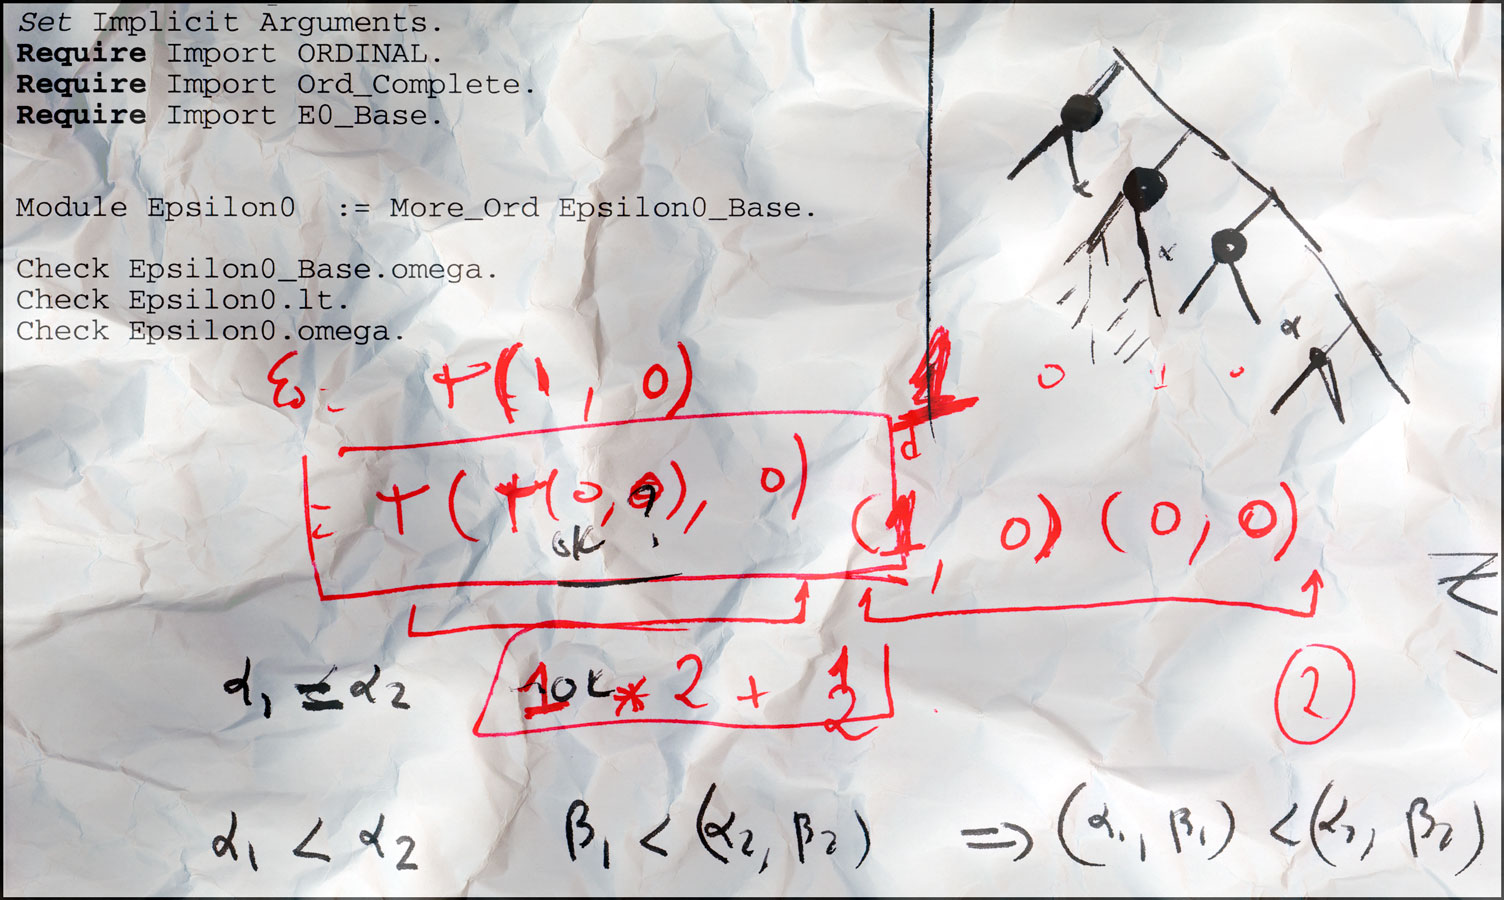
\includegraphics[width=11cm]{epsilon0.jpg}
  \caption{Veblen normal form}
  \label{fig:gamma0}
\end{figure}

Like in chapter~\ref{chap:T1}, we get familiar with the type \texttt{T2} by recognising simple constructs like finite ordinals, $\omega$, etc., as inhabitants of \texttt{T2}.

\begin{Coqsrc}
Notation  "'one'"  := [zero,zero] : T2_scope.

(** The (n+1)-th finite ordinal *)
Notation "'FS' n" := (gcons zero zero n zero) (at level 10) : T2_scope.

(** the [n]-th ordinal  *)
Definition fin (n:nat) := match n with 0 => zero | S p => FS p end.

Notation "'omega'"  := [zero,one] : T2_scope.
\end{Coqsrc}


\begin{Coqsrc}
Notation "'epsilon0'"  := ([one,zero]) : T2_scope.

Definition epsilon alpha := [one, alpha].
\end{Coqsrc}

\section{How Big is \texorpdfstring{$\Gamma_0$}{\texttt{Gamma0}}?}

Let us define a strict order on type \texttt{T2}. The following definition is 
an adaptation of Schütte's, taking into account the multiplications by a natural number (inspired by~\cite{Manolios2005}, and also present in \texttt{T1}).

\label{sect:t2-lt-def}

\begin{Coqsrc}
Inductive lt : T2 -> T2 -> Prop :=
| (* 1 *) 
 lt_1 : forall alpha beta n gamma,  zero t2< gcons alpha beta n gamma
| (* 2 *)
 lt_2 : forall alpha1 alpha2 beta1 beta2 n1 n2 gamma1 gamma2, 
                alpha1 t2< alpha2 ->
                beta1 t2< gcons alpha2 beta2 0 zero ->
               gcons alpha1 beta1 n1 gamma1 t2<
               gcons alpha2 beta2 n2 gamma2
| (* 3 *)
 lt_3 : forall alpha1  beta1 beta2 n1 n2 gamma1 gamma2, 
               beta1 t2< beta2 ->
               gcons alpha1 beta1 n1 gamma1 t2<
               gcons alpha1 beta2 n2 gamma2

| (* 4 *)
 lt_4 : forall alpha1 alpha2 beta1 beta2 n1 n2 gamma1 gamma2, 
               alpha2 t2< alpha1 ->
               [alpha1, beta1] t2< beta2 ->
               gcons alpha1 beta1 n1 gamma1 t2<
               gcons alpha2 beta2 n2 gamma2

| (* 5 *)
lt_5 : forall alpha1 alpha2 beta1 n1 n2 gamma1 gamma2, 
               alpha2 t2< alpha1 ->
               gcons alpha1 beta1 n1 gamma1 t2<
               gcons alpha2  [alpha1, beta1] n2 gamma2

| (* 6 *)
lt_6 : forall alpha1 beta1  n1  n2 gamma1 gamma2,  (n1 < n2)%nat ->
                                    gcons alpha1 beta1 n1 gamma1 t2< 
                                    gcons alpha1 beta1 n2 gamma2

| (* 7 *)
  lt_7 : forall alpha1 beta1 n1   gamma1 gamma2,  gamma1 t2< gamma2 ->
                                      gcons alpha1 beta1 n1 gamma1 t2<
                                      gcons alpha1 beta1 n1 gamma2
where  "o1 t2< o2" := (lt o1 o2): T2_scope.

Hint Constructors lt : T2.
\end{Coqsrc}

Seven constructors! In order to get accustomed with this definition, let us look at a small set of examples, covering all the constructors of \texttt{lt}.


\subsection{Examples}

\subsubsection*{Proof of $0<\epsilon_0$}

\begin{Coqsrc}
Example Ex1: 0 t2< epsilon0.
Proof.  constructor 1. Qed.
\end{Coqsrc}

\subsubsection*{Proof of $\omega<\epsilon_0$}

\begin{Coqsrc}
Example Ex2: omega t2< epsilon0.
Proof. info_auto with T2. (* uses lt_1 and lt_2 *) Qed.
\end{Coqsrc}

\subsubsection*{Proof of $\psi(\omega,8)\times 13+56 < \psi(\omega,8)\times 13+57 $}

\begin{Coqsrc}
Example Ex3: gcons omega 8 12 56 t2<  gcons omega 8 12 57.
Proof.
  constructor 7; constructor 6; auto with arith.
Qed.
\end{Coqsrc}

\subsubsection*{Proof of $\epsilon_0<\psi(2,1)$}

\begin{Coqsrc}
Example Ex4: epsilon0 t2< [2,1].
Proof.
   constructor 2; auto with T2.
   - constructor 6; auto with arith.
Qed.
\end{Coqsrc}

\subsubsection*{Proof of $\psi(2,1)<\psi(2,3)$}

\begin{Coqsrc}
Example Ex5 : [2,1] t2< [2,3].
Proof.
  constructor 3; auto with T2.
  - constructor 6; auto with arith.
Qed.
\end{Coqsrc}

\subsubsection*{Proof of $\psi(1,0)\times 13+ \omega < \psi(0,\psi(2,1))$}
\label{sect:ex6-first-proof}

\begin{Coqsrc}
Example Ex6 : gcons 1 0 12 omega t2< [0,[2,1]].
Proof.
  constructor 4.
  - constructor 1.
  - constructor 2.
    + constructor 6; auto with arith.
    + constructor 1.
Qed.
\end{Coqsrc}

\subsubsection*{Proof of $\psi(2,1)\times 43 + \epsilon_0 < \psi(1,\psi(2,1))$}

\begin{Coqsrc}
Example Ex7 : gcons 2 1 42 epsilon0 t2< [1, [2,1]].
Proof.
 constructor 5.
 constructor 6; auto with arith.
Qed.
\end{Coqsrc}

\index{hydras}{Projects}
\begin{project}
Write a tactic that solves automatically goals of the form (\texttt{$\alpha$ t2< $\beta$}), where $\alpha$ and $\beta$ are closed terms of type \texttt{T2}.
\end{project}

\section{Veblen Normal Forms}
\begin{definition}
  A term of the form $\psi(\alpha_1,\beta_1)\times n_1+ \psi(\alpha_2,\beta_2)\times n_2+\dots+\psi(\alpha_k,\beta_k)\times n_k$ is said to be in
 \emph{[Veblen] normal form} if for every $i<n$, $\psi(\alpha_i,\beta_i)<\psi(\alpha_{i+1},\beta_{i+1})$, all the $\alpha_i$ and $\beta_i$ are in normal form, and all the $n_i$ are strictly positive integers.
\end{definition}

\begin{Coqsrc}
Inductive nf : T2 -> Prop :=
| zero_nf : nf zero
| single_nf : forall a b n, nf a ->  nf b -> nf (gcons a b n zero)
| gcons_nf : forall a b n a' b' n' c', 
                      [a', b'] t2< [a, b]  -> 
                      nf a -> nf b -> 
                      nf(gcons a' b' n' c')-> 
                      nf(gcons a b n (gcons a' b' n' c')).
\end{Coqsrc}

Let us look at some positive examples (we have to prove some inversion lemmas before proving counter-examples).


\begin{Coqsrc}
Lemma  nf_fin i : nf (fin i).
Proof.
  destruct i.
  - auto with T2.
  - constructor 2; auto with T2.
Qed.

Lemma nf_omega : nf omega.
Proof.  compute; auto with T2. Qed.

Lemma nf_epsilon0 : nf epsilon0.
Proof. constructor 2; auto with T2. Qed.

Lemma nf_epsilon : forall alpha, nf alpha -> nf (epsilon alpha).
Proof. compute; auto with T2. Qed.

Example Ex8: nf (gcons 2 1 42 epsilon0).
Proof.
  constructor 3; auto with T2.
  - apply Ex4.
  - apply nf_fin.
  - apply nf_fin.
Qed.
\end{Coqsrc}


\subsection{Length of a Term}

The notion of \emph{term length} is introduced by Schütte as a helper for proving (at least) the \emph{trichotomy} property and transitivity of the strict order \texttt{lt} on \texttt{T2}. These properties are proved by induction on length.

\begin{Coqsrc}
Fixpoint nbterms (t:T2) : nat :=
  match t with zero => 0
             | gcons a b n v => (S n) + nbterms v
  end.

Fixpoint t2_length (t:T2) : nat :=
  match t  with 
    zero => 0
  | gcons a b n v => 
       nbterms (gcons a b n v) + 
      2 * (Max.max (t2_length a)
                              (Max.max (t2_length b) 
                                                (t2_length_aux v)))
  end
with t2_length_aux (t:T2) : nat :=
 match t with 
 | zero => 0
  | gcons a b n v =>
           Max.max (t2_length a) 
                            (Max.max (t2_length b) (t2_length_aux v))
 end.
\end{Coqsrc}

\begin{Coqsrc}
Compute t2_length (gcons 2 1 42 epsilon0).
\end{Coqsrc}

\begin{Coqanswer}
 = 48 : nat
\end{Coqanswer}

\subsection{Trichotomy}

\emph{Trichotomy} is another name for the well-known property of decidable total ordering (like Standard Library's \texttt{Compare\_dec.lt\_eq\_lt\_dec}).

We first prove by induction on $l$ the following lemma:

\vspace{4pt}

\noindent\emph{From \href{../theories/html/hydras.Gamma0.Gamma0\#tricho_aux}%
{\texttt{Gamma0.Gamma0}}}

\begin{Coqsrc}
Lemma tricho_aux (l: nat) : forall t t' :T2,
      t2_length t + t2_length t' < l  ->
      {t t2< t'} + {t = t'} + {t' t2<  t}.
\end{Coqsrc}

Then we get our version of \texttt{lt\_eq\_lt\_dec}, and derive a comparison function;

\begin{Coqsrc}
Definition lt_eq_lt_dec (t t': T2) : {t t2< t'}+{t = t'}+{t' t2<  t}.
Proof.
  eapply tricho_aux.
  eapply lt_n_Sn.
Defined.

Definition compare (t1 t2 : T2) : comparison := 
  match lt_eq_lt_dec t1 t2 with
  | inleft (left _) => Lt
  | inleft (right _) => Eq
  | inright _ => Gt
  end.
\end{Coqsrc}

With the help of \texttt{compare}, we get a boolean version of \texttt{nf}
(being in Veblen normal form).

\begin{Coqsrc}
Fixpoint nfb (alpha : T2) : bool :=
  match alpha with
    zero => true
  | gcons a b n zero => andb (nfb a) (nfb b)
  | gcons a b n ((gcons a' b' n' c') as c) =>
    match compare [a', b'] [a, b] with
           Lt => andb (nfb a) (andb (nfb b) (nfb c))
           | _ => false
           end
end.
\end{Coqsrc}


\begin{Coqsrc}
Compute compare (gcons 2 1 42 epsilon0) [2,2].
\end{Coqsrc}

\begin{Coqanswer}
   = Lt
     : comparison
\end{Coqanswer}

\begin{Coqsrc}
Compute nfb  (gcons 2 1 42 epsilon0).
\end{Coqsrc}

\begin{Coqanswer}
   = true
     : bool
\end{Coqanswer}

\begin{Coqsrc}
Compute nfb (gcons 2 1 42 (gcons 2 2 4 epsilon0)).
\end{Coqsrc}

\begin{Coqanswer}
   = false
     : bool
\end{Coqanswer}

\begin{remark}
The connexion between the predicate \texttt{nf} and the relation \texttt{lt} on one part, and the functions \texttt{nfb} and \texttt{compare} on the other, is expressed by the following lemmas:

\begin{Coqsrc}
Lemma nfb_equiv gamma : nfb gamma = true <-> nf gamma.

Lemma compare_correct alpha beta :
  CompareSpec (alpha = beta) (lt alpha beta) (lt beta alpha)
              (compare alpha beta).
\end{Coqsrc}

The function \texttt{compare} helps to make easier proofs of inequalities of
closed terms of type \texttt{T2}.

First, we prove a lemma:

\begin{Coqsrc}
Lemma compare_Lt : forall alpha beta, compare alpha beta = Lt -> 
                                         alpha t2< beta.
Proof.
  intros alpha beta; destruct (compare_correct alpha beta);
    trivial; discriminate. 
Qed.
\end{Coqsrc}

Then, we give another version of the proof of Sect.~\vref{sect:ex6-first-proof}.

\begin{Coqsrc}
Example Ex6 : gcons 1 0 12 omega t2< [0,[2,1]].
Proof. now apply compare_Lt. Qed.
\end{Coqsrc}

\end{remark}


\section{Main Functions on \texttt{T2}}

\subsection{Successor}
The successor function is defined by structural recursion.

\noindent\emph{From \href{../theories/html/hydras.Gamma0.T2.html\#succ}%
{\texttt{Gamma0.T2}}}
\begin{Coqsrc}
Fixpoint succ (a:T2) : T2 :=
 match a with zero => one
             | gcons zero zero n c => fin (S (S n))
             | gcons a b n c => gcons a b n (succ c)
 end.
\end{Coqsrc}

\subsection{Addition}

Like for Cantor normal forms (see Sect.~\ref{sect:infix-plus-T1}),  the definition of addition in \texttt{T2}  requires comparison between ordinal terms.


\begin{Coqsrc}
Fixpoint plus (t1 t2 : T2) {struct t1}:T2 :=
  match t1,t2 with
  |  zero, y  => y
  |  x, zero => x
  |  gcons a b n c, gcons a' b' n' c' =>
     (match compare (gcons a b 0 zero)
                    (gcons a' b' 0 zero) with
      | Lt => gcons a' b' n' c'
      | Gt => gcons a b n (c + gcons a' b' n' c')
      | Eq => gcons a b (S(n+n')) c'
      end)
  end
where "alpha + beta" := (plus alpha beta): T2_scope.
\end{Coqsrc}

\begin{Coqsrc}
Example Ex7 : 3 + epsilon0 = epsilon0.
Proof. trivial. Qed.
\end{Coqsrc}

\subsection{The Veblen Function \texorpdfstring{$\phi$}{\texttt{phi}}}

The enumeration function of critical ordinals, presented in Sect.~\vref{sect:phi-schutte}, is recursively defined in type \texttt{T2}.

\begin{Coqsrc}
Definition  phi (alpha beta : T2) : T2 :=
  match beta with zero => [alpha, beta] 
             | [b1, b2] => 
               (match compare alpha b1
                with Datatypes.Lt => [b1, b2 ]
                | _ => [alpha,[b1, b2]]
                end)
             | gcons b1 b2 0 (gcons zero zero  n zero) => 
               (match compare alpha b1
                with  Datatypes.Lt => 
                      [alpha, (gcons b1 b2 0 (fin n))]
                | _ =>  [alpha, (gcons b1 b2 0 (fin (S n)))]
                end)
             | any_beta => [alpha, any_beta]
  end.
\end{Coqsrc}

Despite its complexity, the function \texttt{phi} is well adapted to proofs by simplification or computation.
\begin{Coqsrc}
Example Ex8:  phi 1 (succ epsilon0) = [1, [1,0] + 1].
Proof. reflexivity. Qed.
\end{Coqsrc}

\begin{Coqsrc}
(**  All epsilons are fixpoints of phi 0 *)

Theorem epsilon_fxp : forall beta, phi zero (epsilon beta) =
                                   epsilon beta.
Proof. reflexivity. Qed.

Theorem epsilon0_fxp : epsilon0 = phi zero epsilon0.
Proof. apply epsilon_fxp. Qed.
\end{Coqsrc}


The relation between the constructor $\psi$ and the function $\phi$ is
studied in~\cite{schutte}, and partially implemented in this development.
\emph{Please contribute!}
 
For instance, the following theorem states that, if $\gamma$ is the sum of a limit ordinal $\beta$ and a finite ordinal $n$, and $\beta$ is a fixpoint of
$\phi(\alpha)$, then $\psi(\alpha,\gamma)=\phi_\alpha(\gamma+1)$.

\begin{Coqanswer}
phi_psi :
forall (alpha : T2) [beta gamma : T2] [n : nat],
nf gamma ->
limit_plus_fin beta n gamma ->
phi alpha beta = beta -> [alpha, gamma] = phi alpha (succ gamma)
\end{Coqanswer}

\begin{Coqsrc}
Example Ex9 : [zero, epsilon 2 + 4] = phi 0 (epsilon 2 + 5).
Proof. trivial. Qed.
\end{Coqsrc}

On the other hand, $\phi$ can be expressed in terms of $\psi$.

\begin{Coqanswer}
phi_of_psi:
  forall a b1 b2 : T2,
  phi a [b1, b2] = (if lt_ge_dec a b1 then [b1, b2] else [a, [b1, b2]])
\end{Coqanswer}

\begin{Coqsrc}
Example Ex10 : phi omega [epsilon0, 5] = [epsilon0, 5].
Proof. reflexivity. Qed.
\end{Coqsrc}

\index{hydras}{Projects}
\begin{project}
Please study a way to pretty print ordinal terms in Veblen normal form (see Section~\vref{sect:ppT1}).
\end{project}

\section{An Ordinal Notation for \texorpdfstring{$\Gamma_0$}{\texttt{Gamma0}}}

In order to consider type \texttt{T2} as an ordinal notation, we have to build an instance of class \texttt{ON} (See Definition page~\pageref{types:ON}).

First, we define a type that contains only terms in Veblen normal form, and redefine \texttt{lt} and \texttt{compare} by delegation (see for comparison the construction of type \texttt{E0} in Sect.~\vref{sect:E0-def}).

\begin{Coqsrc}
Module G0.

Class G0 := mkg0 {vnf : T2; vnf_ok : nfb vnf}.

Definition lt (alpha beta : G0) := T2.lt (@vnf alpha) (@vnf beta).

Definition compare alpha beta := Gamma0.compare (@vnf alpha) (@vnf beta).
\end{Coqsrc}

Then, we prove that \texttt{lt} is a well-founded strict order and that the
function \texttt{compare} is correct.

\begin{Coqsrc}
Instance lt_sto : StrictOrder lt.

Lemma lt_wf : well_founded lt.

Lemma compare_correct alpha beta :
  CompareSpec (alpha = beta) (lt alpha beta) (lt beta alpha)
              (compare alpha beta).

Instance Gamma0: ON lt  compare.
Proof.
  split.
  - apply lt_sto.
  - apply lt_wf. 
  - apply compare_correct.
Qed.
\end{Coqsrc}


\begin{remark}
The proof of \texttt{lt\_wf} has been written by \'Evelyne Contejean, using her library on the recursive path ordering (see also remark~\vref{remark:a3pat}).
\end{remark}

\index{hydras}{Projects}
\begin{project}
Prove that \texttt{Epsilon0} (page~\pageref{instance-epsilon0})
is a sub-notation system of \texttt{Gamma0}.

Prove that the implemantations of \texttt{succ}, \texttt{+}, $\phi_0$, etc.
are compatible in both notation systems.

Note that a function \texttt{T1\_inj} from \texttt{T1} to \texttt{T2} has already been defined. It may help to complete the task.



\noindent\emph{From \href{../theories/html/hydras.Gamma0.T2.html\#T1_to_T2}%
{\texttt{Gamma0.T2}}}
\begin{Coqsrc}
(* injection from T1 *)

Fixpoint T1_to_T2 (alpha :T1) : T2 :=
  match alpha  with
  | T1.zero => zero
  | T1.ocons a n b => gcons zero (T1_to_T2 a) n (T1_to_T2 b)
  end.
\end{Coqsrc}

\end{project}

\begin{project}
Prove that the notation system \texttt{Gamma0} is a correct implementation 
of the segment $[0,\Gamma_0)$ of the set of countable ordinals.
\end{project}







\chapter{Primitive recursive functions}
\label{chapter:primrec}

\section{Introduction}
Primitive recursive functions are a small class of total functions, corresponding to the expressive power of a simple imperative programming language without \textbf{while} loops, in which every program execution terminates.

Primitive recursive functions are total functions from $\mathbb{N}^n$ to
$\mathbb{N}$, for some $n\in\mathbb{N}$. Note that not all 
total $n$-ary recursive functions are primitive recursive
(see for instance Sect.~\vref{sect:ack-not-PR}).

The traditional definition of the set of primitive recursive functions is structured as an inductive definition 
in five rules: three base cases, and two recursive construction rules. 

\begin{description}
  \item[zero] the constant function of value $0$ is primitive recursive.
\item[S] The successor function $S:\mathbb{N}\rightarrow\mathbb{N}$ is primitive recursive.
 \item[projections] For any pair $0< i\leq n$, the projection $\pi_{i,n}: \mathbb{N}^n\rightarrow\mathbb{N}$, defined by $\pi_{i,n}(x_1,x_2,\dots,x_{n})=x_i$, is primitive recursive.
\item[composition] For any $n$ and $m$, if $h: \mathbb{N}^m\rightarrow\mathbb{N}$, and
$g_0,\dots, g_{m-1}: \mathbb{N}^n\rightarrow\mathbb{N}$ are primitive recursive of $n$ arguments, then the function which maps any
tuple $(x_0,\dots,x_{n-1})$ to $h(g_0(x0,\dots,x_{n-1}),\dots, g_{m-1}(x0,\dots,x_{n-1})): \mathbb{N}^n\rightarrow\mathbb{N}$ is primitive recursive.
\item[primitive recursion]
If $g: \mathbb{N}^n\rightarrow\mathbb{N}$ and $h: \mathbb{N}^{n+2}\rightarrow\mathbb{N}$ are primitive recursive, then the function from $\mathbb{N}^{n+1}$ into $\mathbb{N}$ defined by
\begin{align}
f(0,x_1,\dots,x_n)&=g(x_1,\dots,x_n)\\
f(S(p),x_1,\dots,x_n)&=h(p,f(p, x_1,\dots,x_n),  x_1,\dots,x_n)
\end{align} 
is primitive recursive.
\end{description}


Please note the use of dots: $\ldots$ in the definition above. 
Dots are not part of \gallina's syntax. Thus, the formal definition of the set of primitive recursive function will have to overcome this representation problem.

  We present in this chapter a formalization of  primitive recursive functions, taken from  Russel O'Connor's formalization in \coq{} of
G\"odel's incompleteness theorems~\cite{OConnor05}.

\begin{remark}
 The theory of primitive recursive function is now hosted in
the \texttt{theories/ordinals/Ackermann} directory.
The specific part on G\"odel's theorem,  is also on
coq-community (\url{https://github.com/coq-community/goedel}) and requires the 
\href{https://github.com/coq-community/pocklington}{Pocklington library} for lemmas on primality.
\end{remark}

This chapter contains some comments on Russel's library, as well as a few extensions.
Contributions (under the form of comments, new examples or exercises) are welcome!. 



\section{First look at the Ackermann library}

O'Connor's library on Gödel's incompleteness theorems contains a little more 
than 45K lines of scripts. The part dedicated to primitive recursive functions and Peano arithmetic is 32K lines long and is originally structured in 38 modules.
Thus, we propose a partial exploration of this library, through examples and exercises. Our additions to the original library --- mainly examples and counter-examples ---,
are stored in the directory \texttt{theories/ordinals/MoreAck}.

In particular, the library \href{../theories/html/hydras.MoreAck.html}{MoreAck.AckNotPR} contains the well-known  proof that the Ackermann function is not primitive recursive (see Section~\vref{sect:ack-not-PR}).
Moreover, the library \href{../theories/html/hydras.Hydra_Theorems.html}{Hydra.Hydra\_Theorems} contains 
a proof that the length of an hydra battle (according to the initial replication factor) is not primitive recursive in general.

\section{Basic definitions}
\index{maths}{Primitive recursive functions}

The formal definition of primitive recursive functions lies in the library
\href{../theories/html/hydras.Ackermann.primRec.html}{Ackermann.primRec},
with preliminary definitions in 
\href{../theories/html/hydras.Ackermann.extEqualNat.html}{Ackermann.extEqualNat}
and
\href{../theories/html/hydras.Ackermann.misc.html}{Ackermann.misc}.

\subsection{Functions of arbitrary arity}

The  \texttt{primRec} library allows us to consider primitive functions on \texttt{nat}, with any number of arguments, in 
curried form. This is made possible in 
\href{../theories/html/hydras.Ackermann.extEqualNat.html}{Ackermann.extEqualNat} by the following definition:

\index{primrec}{Types!naryFunc}
\input{movies/snippets/extEqualNat/naryFunc.tex}

For instance (\texttt{naryFunc 1}) is convertible to \texttt{nat -> nat} and (\texttt{naryFunc 3})
to \texttt{nat -> nat -> nat -> nat}.

\vspace{4pt}
\noindent
\emph{From \href{../theories/html/hydras.MoreAck.PrimRecExamples.html}{MoreAck.PrimRecExamples}}.

\input{movies/snippets/PrimRecExamples/naryFunc3}
\input{movies/snippets/PrimRecExamples/checknaryFunc}


Likewise, arbitrary boolean predicates may have an arbitrary number of arguments. The dependent type
(\texttt{naryRel $n$}), defined in the same way as \texttt{naryFunc}, is the type of $n$-ary functions from
\texttt{nat} into \texttt{bool}.

\input{movies/snippets/PrimRecExamples/naryRel2}

The magic of dependent types makes it possible to define recursively extensional equality between functions of the same arity.

\index{coq}{Dependent types}
\index{coq}{Dependently typed functions}
\vspace{4pt}
\noindent
\emph{From \href{../theories/html/hydras.Ackermann.extEqualNat.html}{Ackermann.extEqualNat}}

\index{primrec}{Predicates!extEqual}

\input{movies/snippets/extEqualNat/extEqualDef}


\input{movies/snippets/PrimRecExamples/extEqual2a}

  Getting rid of the term \texttt{x-x}, we generate two easy-to-solve subgoals.

\vspace{6pt}
\noindent
\input{movies/snippets/PrimRecExamples/extEqual2b}
  
\subsection{A Data-type for Primitive Recursive Functions}

O'Connor's formalization of primitive recursive functions takes the form of two mutually inductive dependent data types, each constructor of which is associated with one of these  rules.
These two types are (\texttt{PrimRec $n$}) (primitive recursive functions of $n$ arguments), and
(\texttt{PrimRecs $n$ $m$}) ($m$-tuples of primitive recursive functions of $n$ arguments).


\index{coq}{Dependent types}
\index{coq}{Mutually inductive types}

\index{primrec}{Types!PrimRec}
\index{primrec}{Types!PrimRecs}
\label{def:Primrec}
\vspace{4pt}
\noindent
\emph{From \href{../theories/html/hydras.Ackermann.primRec.html}{Ackermann.primRec}.}

\input{movies/snippets/primRec/PrimRecDef}

\begin{remark}
\label{projFunc-order-of-args}
Beware of the conventions used in the \texttt{primRec} library!
The constructor (\texttt{projFunc $n$ $m$})  is associated with the projection $\pi_{n-m,n}$ and \emph{not}
$\pi_{n, m}$.
For instance, the projection $\pi_{2,5}$ defined by $\pi_{2,5}(a,b,c,d,e)=b$ corresponds to the term
(\texttt{projFunc 5 3 H}), where \texttt{H} is a proof of $3<5$.
 This fact is reported in the comments of \texttt{primRec.v}. We presume that this convention makes it easier to define the evaluation function (\texttt{evalProjFunc $n$}) (see the next sub-section). Trying the other convention is left as an exercise.
\end{remark}



\subsection{A little bit of semantics} 
Please note that inhabitants of type (\texttt{PrimRec $n$}) are not \coq{} functions like \texttt{Nat.mul}, or factorial, etc. The data-type (\texttt{PrimRec $n$}) is indeed an abstract syntax for the language of primitive recursive functions. The bridge between this language and the word of usual functions
is an interpretation function (\texttt{evalprimRec $n$})  of type
$\texttt{PrimRec}\,n \rightarrow  \texttt{naryFunc}\,n$.
This function is defined by mutual recursion,  together with the  function 
(\texttt{evalprimRecS $n$ $m$}) of type 
$\texttt{PrimRecs}\,n\,m \rightarrow  \texttt{Vector.t}\,(\texttt{naryFunc}\,n)\,m$.

\index{primrec}{Functions!evalPrimRec}
\index{primrec}{Functions!evalPrimRecs}

\index{coq}{Dependent pattern matching}
Both functions are mutually defined through dependent pattern matching. We advise the readers who 
would feel uneasy with dependent types to consult Adam Chlipala's \emph{cpdt}  book~\cite{chlipalacpdt2011}. We leave it to the reader  to look also at the helper functions in
\href{../theories/html/hydras.Ackermann.primRec.html}{Ackermann.primRec}.

\vspace{4pt}

\input{movies/snippets/primRec/evalPrimRecDef}

\vspace{4pt}

Looks complicated? The following examples show that, when
the arity is fixed, these definitions behave well w.r.t. 
\coq's reduction rules. Moreover, they make the interpretation functions more ``concrete''.

\vspace{4pt}
\noindent
\emph{From \href{../theories/html/hydras.MoreAck.PrimRecExamples.html}{MoreAck.PrimRecExamples}.}

\input{movies/snippets/PrimRecExamples/evalPrimRecEx}

\vspace{4pt}
\noindent

Another example?
Let us consider the following term\footnote{Of course, we never typed this term \emph{verbatim}; we obtained it by an interactive proof the reader will be able to make after 
reading Sect.\vref{sect:proofs-of-isPR}.}:

\label{sect:bigfac}

\input{movies/snippets/PrimRecExamples/bigPRa}


Let us now interpret this term as an arithmetic function.

\vspace{4pt}
\noindent

\input{movies/snippets/PrimRecExamples/bigPRb}


After this test, the term \texttt{bigPR} looks to be a primitive recursive definition of the factorial function, although we haven't proved this fact yet. Fortunately, we will see in the following sections simple ways to prove that a given function is primitive recursive, without building such an unreadable term.

\section{Proving that a given arithmetic function is primitive recursive}
\label{sect:proofs-of-isPR}

The example in the preceding section clearly shows that, in order to prove that a given arithmetic function
(defined in \gallina{} as usual) is primitive recursive, trying to give  by hand a term  of type (\texttt{PrimRec $n$}) is not a good method, since such terms may be huge and complex, even for simple arithmetic functions. The method proposed in Library \texttt{primRec} is the following one:

\begin{enumerate}
\item Define a type corresponding to the statement "the function \texttt{$f$:naryFunc $n$} is primitive recursive ''.
\item Prove handy lemmas which may help to prove that a given function is primitive recursive.
\end{enumerate}

Thus, the proof that a function, like \texttt{factorial}, is primitive recursive may be interactive, without having to type complex terms at any step of the development.

\subsection{The predicate \texttt{isPR}}

\index{primrec}{Predicates!isPR}
%\index{coq}{Extensionally equal functions}

Let $f$ be an arithmetic function of arity $n$. We say that $f$ is primitive recursive if $f$ is \textbf{extensionally}
equal to the interpretation of some term of type \texttt{PrimRec $n$}. 

\vspace{4pt}
\noindent
\emph{From \href{../theories/html/hydras.Ackermann.primRec.html}{Ackermann.primRec}.}

\input{movies/snippets/primRec/isPRDef}

The library \texttt{primRec} contains a large catalogue of lemmas allowing to prove statements 
of the form (\texttt{isPR $n$ $f$}). We won't list all these lemmas here, but give a few examples of
how they may be applied.

\begin{remark}
In the library \texttt{primRec}, all these lemmas are opaque (registered with \texttt{Qed}). Thus they do not allow the user to look at the witness of a proof of a \texttt{isPR} statement. Our example of page~\pageref{sect:bigfac} was built using a  copy of \texttt{primRec.v} where many \texttt{Qed}s have been replaced with
\texttt{Defined}s.

If it does not cause compatibility problems (with 
\href{https://github.com/coq-community/goedel}{goedel library} for instance), we plan to make all theses lemmas transparent.
\end{remark}

\subsubsection{Elementary proofs of \texttt{isPR} statements}

The constructors \texttt{zeroFunc}, \texttt{succFunc},  and \texttt{projFunc} of type
\texttt{PrimRec} allows us to write trivial proofs of primitive recursivity. 
Some of   the following lemmas are already proven in 
\href{../theories/html/hydras.Ackermann.primRec.html}{Ackermann.primRec}. More examples are given in 
\href{../theories/html/hydras.MoreAck.PrimRecExamples.html}%
{Ackermann.MoreAck.PrimRecExamples.v}, in order to illustrate the main proof patterns.

\input{movies/snippets/PrimRecExamples/zeroIsPR}


Likewise, we prove that the successor function on \texttt{nat} is primitive recursive too.

\input{movies/snippets/primRec/SuccIsPR}



Projections are proved primitive recursive, case by case (many examples in 
\href{../theories/html/hydras.Ackermann.primRec.html}{Ackermann.primRec}).
\emph{Please notice again that the name of the projection follows the mathematical tradition, 
whilst the arguments of  \texttt{projFunc} use another convention (\emph{cf} remark~\vref{projFunc-order-of-args}).}


\input{movies/snippets/PrimRecExamples/pi25IsPR}



Please note that the projection $\pi_{1,1}$ is just the identity on \texttt{nat}, and is realized by 
(\texttt{projFunc 1 0}).


\vspace{4pt}
\noindent
\emph{From \href{../theories/html/hydras.Ackermann.primRec.html}{Ackermann.primRec}.}

\input{movies/snippets/primRec/idIsPR}

\subsubsection{Using function composition}

Let us look at the proof that any constant $n$ of type \texttt{nat} has type (\texttt{PR 0})
(lemma  \texttt{const1\_NIsPR} of \texttt{primRec}). We carry out a proof by induction on $n$, the base case of which is already proven.
Now, let us assume $n$ is \texttt{PR $n$}, with $x:\texttt{PrimRec}\,0$ as a ``realizer''.
Thus we would like to compose this constant function with the unary successor function.

This is exactly the role of the instance \texttt{composeFunc 0 1} of the dependently typed
function \texttt{composeFunc}, as shown by the following lemma.

\vspace{4pt}
\input{movies/snippets/PrimRecExamples/compose01}


\vspace{4pt}
Thus, we get a quite simple proof of \texttt{const1\_NIsPR}.


\vspace{4pt}
\noindent
\emph{From \href{../theories/html/hydras.MoreAck.PrimRecExamples.html}{MoreAck.PrimRecExamples}}.

\input{movies/snippets/PrimRecExamples/const0NIsPR}

\subsubsection{Proving that \texttt{plus} is primitive recursive}

The lemma \texttt{plusIsPR} is already proven in \href{../theories/html/hydras.Ackermann.primRec.html}{Ackermann.primRec}. We present in 
\href{../theories/html/hydras.MoreAck.PrimRecExamples.html}{MoreAck.PrimRecExamples}
a commented version of this proof, 

First, we look for lemmas which may help to prove that a given function obtained with the recursor \texttt{nat\_rec} is primitive recursive.

\input{movies/snippets/PrimRecExamples/PrimRecExamplesSearch}

The following lemma shows it suffices to prove that
Standard library's function \texttt{plus} is extensionally equal to a function defined with
\texttt{nat\_rec}.

\input{movies/snippets/PrimRecExamples/isPRExtEqualTrans}

Thus, let us define an helper and prove its equivalence with \texttt{plus}.

\input{movies/snippets/PrimRecExamples/plusAlt}


\vspace{4pt}


We are now able to complete the proof.

\input{movies/snippets/PrimRecExamples/plusIsPRa}


We already proved that \texttt{S} is \texttt{PR 1}, but we need to consider a function of three arguments, which ignores its first and third arguments.
Fortunately, the library \texttt{primRec} already contains lemmas adapted to this kind of situation.

\vspace{4pt}
\input{movies/snippets/PrimRecExamples/checkFilter0101IsPR}
\vspace{4pt}


Thus, our first subgoal is solved easily. The rest of the proof 
is just an application of already proven lemmas.

\vspace{4pt}

\input{movies/snippets/PrimRecExamples/plusIsPRb}


\begin{todo}
Comment more examples from   \href{../theories/html/hydras.MoreAck.PrimRecExamples.html}{MoreAck.PrimRecExamples}.
\end{todo}

\index{primrec}{Exercises}
\begin{exercise}
There is a lot of lemmas similar to \texttt{filter010IsPR} in the \texttt{primRec} library, useful to control the arity of functions.
Thus, the reader may look at them, and invent simple examples of application for each lemma.
\end{exercise}

\index{primrec}{Exercises}
\begin{exercise}
Multiplication of natural number is already proven in the \texttt{primRec} library. Write a proof of your own, then compare to the library's version.
\end{exercise}

%\input{movies/snippets/PrimRecExamples/justATest}

\subsubsection{More examples}

The following proof decomposes the \texttt{double} function as the composition of 
multiplication with the identity and the constant function which returns $2$.
\emph{Note that the lemma \texttt{const1\_NIsPR} considers this function as an unary function (unlike \texttt{const0\_NIsPR})}. 
\input{movies/snippets/PrimRecExamples/doubleIsPRa}

\input{movies/snippets/PrimRecExamples/doubleIsPRb}

\index{primrec}{Exercises}
\begin{exercise}
Prove that the following functions are primitive recursive. 

\input{movies/snippets/MorePRExamples/factDef}

\input{movies/snippets/MorePRExamples/expDef}

\input{movies/snippets/MorePRExamples/tower2Def}


\textbf{Hint:} You may have to look again at the lemmas of the library
\href{../theories/html/hydras.Ackermann.primRec.html}{Ackermann.primRec} if you meet some difficulty.
You may start this exercise with the file
    \href{https://github.com/coq-community/hydra-battles/blob/master/exercises/primrec/MorePRExamples.v}{exercises/primrec/MorePRExamples.v}.
\end{exercise}



\index{primrec}{Exercises}
\begin{exercise}
Show that the function \texttt{min: naryFunc\,2} is primitive
recursive.

\emph{You may start this exercise with
    \href{https://github.com/coq-community/hydra-battles/blob/master/exercises/primrec/MinPR.v}{exercises/primrec/MinPR.v}.}

\end{exercise}

\index{primrec}{Exercises}

\begin{exercise}
Write a simple and readable proof that the Fibonacci function is primitive recursive.

\input{movies/snippets/FibonacciPR/fibDef}


\textbf{Hint:}  You may use as a helper the function which computes the pair \linebreak
$(\texttt{fib}(n+1),\texttt{fib}(n))$. 
Library \href{../theories/html/hydras.Ackermann.cPair.html}{Ackermann.cPair} contains
the definition of the encoding of $\mathbb{N}^2$ into $\mathbb{N}$, and the proofs that 
the associated constructor and projections are primitive recursive.  
\emph{You may start this exercise with the file
  \href{https://github.com/coq-community/hydra-battles/blob/master/exercises/primrec/FibonacciPR.v}{exercises/primrec/FibonacciPR.v}.}

\vspace{4pt}

\emph{See also the chapter~\ref{chap:encoding} on G\"{o}del's encodings.}

\end{exercise}

\index{primrec}{Exercises}
\begin{exercise}

Prove the following lemmas (which may help to solve the next  exercise).

\inputsnippets{isqrt/boundedSearch3, isqrt/boundedSearch4}

\textbf{Note:}  The function \texttt{boundedSearch} is defined
in Library \href{../theories/html/hydras.Ackermann.primRec.html}{Ackermann.primRec}. 
\end{exercise}

\index{primrec}{Exercises}

\begin{exercise}
Prove that the function which returns the  integer square root of any natural number  is primitive recursive.

\emph{You may start this exercise with the file
    \href{https://github.com/coq-community/hydra-battles/blob/master/exercises/primrec/isqrt.v}{exercises/primrec/isqrt.v}.}

\end{exercise}

\section{Proving that a given function is \emph{not} primitive recursive}
\label{sect:ack-not-PR}

The best known example of a total recursive function which is not primitive recursive is the Ackermann function. We show how to adapt the classic proof (see for instance~\cite{planetmath}) to the constraints of \gallina. We hope this formal proof 
 is a nice opportunity to explore
the treatment of primitive recursive functions by R. O'Connor,
and to play with dependent types.

\subsection{Ackermann function}

Ackermann function is traditionally defined as a function from 
$\mathbb{N}\times \mathbb{N}$ into $\mathbb{N}$, through
three equations:

\begin{align}
A(0,n)&=n+1\\
A(m+1,0)&=A(m,1)\\
A(m+1,n+1)&=A(m,A(m+1,n))
\end{align}

Let us try to define this function in \coq{} (in curried form).

\input{movies/snippets/Ack/AckFixpointFail.tex}

A possible workaround is to make \texttt{m} be the 
decreasing argument, and define --- within \texttt{m}'s scope --- a local helper function which computes (\texttt{Ack m n}) for any \texttt{n}.
This way, both functions \texttt{Ack} and \texttt{Ackm} have a (structurally) strictly decreasing argument.

\input{movies/snippets/Ack/AckFixpointAlt.tex}

We preferred to define a variant which uses explicitly
 the functional \texttt{iterate},
where (\texttt{iterate\,$f$\,$n$})
is the $n$-th iteration of $f$\,\footnote{Please not confuse with \texttt{primRec.iterate}, which is monomorphic and does not share the same order of arguments.}. It makes it possible to apply a few lemmas proved in 
\href{../theories/html/hydras.Prelude.Iterates.html}{Prelude.Iterates}, for instance about the monotony of the $n$-th iterate of a given function. 


\vspace{4pt}
\noindent
\emph{From \href{../theories/html/hydras.Prelude.Iterates.html}{Prelude.Iterates}}.
\index{hydras}{Library Prelude!iterate}

\input{movies/snippets/Iterates/iterateDef}

\input{movies/snippets/Iterates/iterateLeNSN}


Thus, our definition of the Ackermann function is as follows:

\vspace{4pt}
\noindent
\emph{From \href{../theories/html/hydras.MoreAck.Ack.html}{MoreAck.Ack}}.
\index{maths}{Ackermann function}
\index{primrec}{Ackermann function}

\input{movies/snippets/Ack/AckFixpointIterate.tex}


\index{hydras}{Exercises}

\begin{exercise}
The file \href{../theories/html/hydras.MoreAck.Ack.html}{MoreAck.Ack} presents two other definitions of the Ackermann functions based on the lexicographic ordering on $\mathbb{N}\times\mathbb{N}$.
Prove that the four functions are extensionally equal.
\end{exercise}


\subsubsection{First properties of the Ackermann function}

The three first lemmas make us sure that our function 
\texttt{Ack} satisfies the ``usual'' equations.

\input{movies/snippets/Ack/AckRewrite}


\vspace{4pt}

The order of growth of the Ackermann function w.r.t. its first argument is illustrated by the following equalities.

\input{movies/snippets/Ack/Ack1N}
\input{movies/snippets/Ack/Ack2N}
\input{movies/snippets/Ack/Ack3N}
\input{movies/snippets/Ack/Ack4N}


\begin{remark}
 The statements above can be rewritten in a more uniform way:

 \begin{quote}
   For $m\in 1..4$, $\texttt{Ack}\,m\,n = f_m\,(n+3)-3$, where 
   \begin{align*}
   f_1(n)=&\,n+2 \\
   f_2(n)=&\,n\times 2\\
   f_3(n)=&\,2^n\\
   f_4(n)=&\,2^{2^{\dots^2}}\quad(n\;\textit{levels})
   \end{align*}
 \end{quote}
\end{remark}


An important property of the Ackermann function helps us 
to overcome the difficulty raised by nested recursion, by climbing up the hierarchy $\texttt{Ack}\,n\,\_\;(n\in\mathbb{N})$.


\noindent
\emph{From \href{../theories/html/hydras.MoreAck.Ack.html}{MoreAck.Ack}}.

\input{movies/snippets/Ack/nestedAckBound}



Please note also that for any given $n$, the unary function
(\texttt{Ack\,$n$}) is primitive recursive.

\vspace{4pt}

\noindent

\emph{From \href{../theories/html/hydras.MoreAck.AckNotPR.html}{MoreAck.AckNotPR}}.

\input{movies/snippets/AckNotPR/AckNIsPR}





\subsection{A proof by induction on all primitive recursive functions}

In order to prove that \texttt{Ack} (considered as a function of two arguments) is not primitive recursive, the usual method consists in two steps:


\begin{enumerate}
\item Prove that for any primitive recursive function $f:\mathbb{N}\rightarrow\mathbb{N}\rightarrow\mathbb{N}$, there exists some natural number $n$ depending on $f$, such that, for any $x$ and $y$, 
$f\,x\,y \leq \texttt{Ack}\,n\,(\textrm{max}\,x\,y)$ (we say that $f$ is \emph{``majorized''}  by \texttt{Ack}).
\item Show that \texttt{Ack} fails to satisfy this property.
\end{enumerate}

First, we prove that any primitive function of two arguments is majorized by \texttt{Ack}.
If we look at the inductive definition of primitive recursive functions, page~\pageref{def:Primrec}, it is obvious that a proof by induction on the construction of primitive recursive functions must consider functions of any arity.

The following scheme allows us to write proofs by induction on the class of primitive recursive functions. 

\vspace{4pt}
\noindent
\emph{From \href{../theories/html/hydras.Ackermann.primRec.html}{Ackermann.primRec}.}


\index{coq}{Commands!Scheme}
 
\inputsnippets{primRec/SchemePrimRecInd,
primRec/SchemePrimRecInda}



Please note that, in order to prove a property shared by any primitive recursive function of, say, arity 2, this induction scheme  leads you to consider an extension of the considered property to primitive recursive function of any arity.

Thus the lemma we will have to prove is the following one:


  \begin{quote}
    For any $n$, and any primitive recursive function $f$ of  arity $n$, there exists some natural number $q$ such that the following inequality holds:
 \[
  \forall x_1,\dots,x_n, 
      f(x_1,\dots,\,x_n)\leq\textrm{Ack}(q,\textrm{max}(x_1,\dots,x_n))
\]
 \end{quote}


But dots don't belong to \gallina's syntax! So, we may use \coq's vectors for denoting arbitrary tuples.

First, we extend \texttt{max} to vectors of natural numbers (using the notations of module \texttt{VectorNotations} and some more definitions from 
\href{../theories/html/hydras.Prelude.MoreVectors.html}{Prelude.MoreVectors}). So, (\texttt{t\,$A$\,$n$}) is the type of vectors of $n$ elements of type $A$, and the constants \texttt{cons}, \texttt{nil}, \texttt{map}, etc., refer to vectors and not to lists. Likewise, the notation \texttt{x::v} is an abbreviation for
\texttt{VectorDef.cons x \_ v}.

\index{coq}{Dependently typed functions}

\input{movies/snippets/MoreVectors/maxvDef}

\input{movies/snippets/MoreVectors/maxvLemmasa}

\input{movies/snippets/MoreVectors/maxvLemmasb}

\input{movies/snippets/MoreVectors/maxvLemmasc}


We have also to convert any application
$(f\,x_1\,x_2\,\dots\,x_n)$ into an application of a function 
to a single argument: the vector of all the $x_i$\,s.
This is already defined in 
Library~\href{../theories/html/hydras.Ackermann.primRec.html}{Ackermann.primRec}.


\input{movies/snippets/primRec/evalListDef}

Indeed, (\texttt{evalList $m$ $v$ $f$}) is the application to the vector $v$ of
an uncurried version of $f$.
In Library\href{../theories/html/hydras.MoreAck.AckNotPR.html}{MoreAck.AckNotPR}, we introduce a lighter notation.

\index{coq}{Dependently typed functions}

\input{movies/snippets/AckNotPR/vApply}



We are now able to translate in \gallina{} the notion of ``majorization'':

\index{coq}{Dependently typed functions}

\input{movies/snippets/AckNotPR/majorizedDefs}


Now, it remains to prove that any primitive function is majorized by \texttt{Ack}.
The three base cases  are as follows:

\input{movies/snippets/AckNotPR/majorSucc}

\input{movies/snippets/AckNotPR/majorZero}

\input{movies/snippets/AckNotPR/majorProjection}



The remaining cases are proved within a mutual  induction.

\index{coq}{Mutual induction}

\input{movies/snippets/AckNotPR/majorAnyPRa}



\input{movies/snippets/AckNotPR/majorAnyPRb}


The last two goals deal with vectors of functions.

\input{movies/snippets/AckNotPR/majorAnyPRVec}


\subsection{Looking for a contradiction}

The following lemma is just a specialization of \texttt{majorAnyPR} to
binary functions (forgetting vectors, coming back to usual notations).

\input{movies/snippets/AckNotPR/majorPR2}

We prove also a strict version of this lemma, thanks to the following property (proved in Library
\href{../theories/html/hydras.MoreAck.Ack.html}{MoreAck.Ack}~).

\input{movies/snippets/Ack/AckStrictMonoL}


\vspace{4pt}
\noindent
\emph{From \href{../theories/html/hydras.MoreAck.AckNotPR.html}{MoreAck.AckNotPR}.}


\input{movies/snippets/AckNotPR/majorPR2Strict}



If the Ackermann function were primitive recursive, then there would exist some natural number $n$, such that, for all $x$ and $y$, the inequality 
$\texttt{Ack}\,x\,y\leq \texttt{Ack}\,n\,(\texttt{max}\,x\,y)$ holds.
Thus, our impossibility proof is just a sequence of easy small steps.

\input{movies/snippets/AckNotPR/AckNotPR}

\begin{remark}
It is easy to prove that any unary function which dominates \texttt{fun n => Ack n n} fails to be primitive recursive. To this end, we use an instance of \texttt{majorAnyPR} dealing with unary functions.

\vspace{4pt}
\noindent

\emph{From \href{../theories/html/hydras.MoreAck.AckNotPR.html}{MoreAck.AckNotPR}}.

\input{movies/snippets/AckNotPR/majorPR1}

Then, we write  a short proof by contradiction.

\input{movies/snippets/AckNotPR/domAckNotPR}

\end{remark}

\begin{remark}
Note that the Ackermann function is a counter-example to the (false) statement:
\begin{quote}
{\color{red}
  ``Let $f$ be a function of type \texttt{naryFunc\,2}. If, for any $n$, the function $f(n)$ is primitive recursive, then f is primitive recursive.''}
\end{quote}
\end{remark}

\subsection{Related work}

This proof is very close to the 1993 proof by Nora Szasz with the \texttt{Alf} proof assistant. This proof has also been adapted
by Lawrence C. Paulson to Isabelle/HOL~\cite{paulson_2021}.

\section{The length of standard hydra battles}
\label{sect:battle-length-notPR}

The module \href{../theories/html/hydras.Hydra.Hydra_Theorems.html}{Hydra\_Theorems} contains a proof that the function which computes the length of standard hydra battles is not primitive recursive. More precisely, we consider, for a given hydra $h=\iota(\alpha)$, the length of a standard battle which starts with the replication factor $k$ (see Sect~\vref{def:L-alpha}).

This proof is  a little more complex than the preceding one.

\subsection{Definitions}

The function we consider is defined and proven correct in
Module~\href{../theories/html/hydras.Hydra.Battle_length.html}{Hydra.Battle\_length}.

\input{movies/snippets/Battle_length/BattleLength}

\subsection{Proof steps}

Now, let us assume that the function \texttt{l\_std} is primitive recursive.


\emph{From \href{../theories/html/hydras.Hydra.Hydra_Theorems.html}{Hydra.Hydra\_Theorems}}.

\input{movies/snippets/Hydra_Theorems/battleLengthNotPRa}

Let us consider the hydra represented by the ordinal $\omega^\omega$.

\input{movies/snippets/Hydra_Theorems/battleLengthNotPRb}


In order to get rid of the subtraction in the definition of \texttt{l\_std}, we work with a helper function.

\input{movies/snippets/Hydra_Theorems/battleLengthNotPRc}

Under the hypothesis \texttt{H}, $m$ is also primitive recursive.

\input{movies/snippets/Hydra_Theorems/battleLengthNotPRd}


\subsubsection{Comparison between $F$ and $H'$}

In \href{../theories/html/hydras.Epsilon0.F_alpha.html}{Epsilon0.F\_alpha}, we prove a relation between the $F$ and $H'$ functionals. For any $\alpha$ and $k>0$,
$H'_{\omega^\alpha}(k)\geq F_\alpha(k)$.

\input{movies/snippets/F_alpha/HprimeF}


Our proof of this lemma is not trivial at all, it uses some properties of the Ketonen-Solovay's toolkit. We advise the reader to explore this proof, with the help of an IDE or software like \alectr.
%%
%%% To move the path chapter
%%%%

% \begin{Coqsrc}
%   alpha : E0
%   IHalpha : forall beta : E0, beta o< alpha -> P beta
%   Halpha : Limitb alpha
%   n : nat
%   ============================
%   H'_ (Phi0 (CanonS alpha n)) (S n) <= 
%   H'_ (Phi0 (CanonS alpha (S n))) (S n)
% \end{Coqsrc}

% In mathematical notation: $H'_{\omega^{\canonseq{\alpha}{n}}}(n+1) \leq
% H'_{\omega^{\canonseq{\alpha}{n+1}}}(n+1)$.

% \vspace{4pt}

% But there exists no lemma saying that, if 
% $\beta\leq \alpha$, then $H'_\beta(k)\leq H'_\alpha(k)$, for any $\alpha$ and $\beta$. For instance, 
% $H'_{42}(3)=45> H'_\omega(3)=7$.


% Looking for lemmas of the form $H'_\beta(k)\leq H'_\alpha(k)$, we find this one (from our library
% \href{../theories/html/hydras.Epsilon0.Hprime.html}{Epsilon0.Hprime}):

% \begin{Coqanswer}
% H'_restricted_mono_l : 
%     forall (alpha beta : E0) (n : nat), 
%       Canon_plus n alpha beta -> 
%       H'_ beta n <= H'_ alpha n.
% \end{Coqanswer}

% Thus, it remains to prove that 
% there exists a path from ${\omega^{\canonseq{\alpha}{n+1}}}$
% to ${\omega^{\canonseq{\alpha}{n}}}$ composed of 
% $n+1$-steps.

% Fortunately, the Ketonen-Solovay machinery contains three lemmas which help us to build such a path.


% \begin{Coqanswer}
% KS_thm_2_4_lemma5 :
%   forall [i : nat] [alpha beta : T1],
%   const_pathS i alpha beta ->
%   nf alpha -> alpha <> zero -> 
%   const_pathS i (phi0 alpha) (phi0 beta)

% KS_thm_2_4 :
%   forall [lambda : T1], nf lambda ->limitb lambda ->
%   forall i j : nat, i < j -> 
%    const_pathS 0 (canonS lambda j) (canonS lambda i)

% Cor12_1 :
% forall [alpha : T1], nf alpha ->
%       forall (beta : T1) (i n : nat),
%       beta t1< alpha ->
%      i <= n -> const_pathS i alpha beta -> 
%      const_pathS n alpha beta
% \end{Coqanswer}
  
\subsubsection{End of the proof}

We finish the proof by comparing several fast growing functions.

\vspace{4pt}

\emph{From \href{../theories/html/hydras.Epsilon0.L_alpha.html}{Epsilon0.L\_alpha}}

\input{movies/snippets/L_alpha/HprimeL}

\vspace{4pt}

\emph{From \href{../theories/html/hydras.Epsilon0.F_omega.html}{Epsilon0.F\_omega}}
\input{movies/snippets/F_omega/FVsAck}

\vspace{4pt}

By transitivity, we get the inequality
$F_\omega(k+1)\leq m(k+1)$, for any $k$.

\input{movies/snippets/Hydra_Theorems/mGeFOmega}


We finish the proof by noting that the function $m$ (composed with \texttt{S}) dominates the Ackermann function, which leads to a contradiction.

\input{movies/snippets/Hydra_Theorems/mDominatesAck}

\input{movies/snippets/Hydra_Theorems/SmNotPR}

\vspace{4pt}

\input{movies/snippets/Hydra_Theorems/LNotPR}




\part{A Few  Certified Algorithms}

\chapter{Smart computation of \texorpdfstring{$x^n$}{Powers}}
\label{chapter-powers}
\section{Introduction}

Nothing looks simpler than writing a function for computing $x^n$.
But on the contrary, this simple programming exercise allows us to address
advanced programming techniques such as:
\begin{itemize}
\item monadic programming, and continuation passing style
\item type classes, and generalized rewriting
\item proof engineering, in particular proof reuse
\item proof by reflection
\item polymorphism and parametricity
\item composition of correct programs, etc.
\end{itemize}



\section{Some basic implementations}
\label{sect:linear-naive}
Let us start with a very naive way of computing the $n$-th power of $x$, where
$n$ is a natural number and $x$ belongs to some type for which a multiplication and an identity element are defined.


\emph{From Module 
\href{../theories/html/additions.FirstSteps.html}{\texttt{additions.FirstSteps}}}
\label{sect: power-definitions}

\begin{Coqsrc}
Section Definitions.

Variables (A: Type)
           (mult: A -> A -> A)
           (one: A).
Local Infix "*" := mult.
Local Notation "1" := one.
\end{Coqsrc}

\begin{Coqsrc}
Fixpoint power (x:A)(n:nat) : A :=
  match n with 
   | 0%nat => 1
   | S p =>   x * x ^ p
  end
where "x ^ n" := (power x n).

\end{Coqsrc}

\begin{Coqsrc}
Compute power Z.mul 1%Z 2%Z 10.  
\end{Coqsrc}
\begin{Coqanswer}
   = 1024%Z
     : Z
\end{Coqanswer}

\begin{Coqsrc}
Open Scope string_scope.
Compute power append  "" "ab"  12.
\end{Coqsrc}
 
 
\begin{Coqanswer}
 = "abababababababababababab"
     : string
\end{Coqanswer}


An application of this function for  computing $x^n$ needs $n$ multiplications.
 Despite this lack of efficiency, and thanks to its simplicity, we keep it as a specification for more efficient and complex exponentiation algorithms.
A function will be considered a \emph{correct} exponentiation function if we can prove it is extensionally equivalent to \texttt{power}.

% \subsection{A semi-naive algorithm}

% In versions up to \texttt{V8.9.1}, the exponentiation function on type \texttt{Z} was defined as follows,
% (in modules \texttt{Coq.PArith.BinPosDef.Pos} and \texttt{Coq.ZArith.BinIntDef.Z}.

% \begin{Coqsrc}
% (** ** Iteration of a function over a positive number *)

% Definition iter {A} (f:A -> A) : A -> positive -> A :=
%   fix iter_fix x n := match n with
%     | xH => f x
%     | xO n' => iter_fix (iter_fix x n') n'
%     | xI n' => f (iter_fix (iter_fix x n') n')
%   end.

% Definition pow (x:positive) := iter (mul x) 1.
% \end{Coqsrc}


% \begin{Coqsrc}
% Definition pow_pos (z:Z) := Pos.iter (mul z) 1.

% Definition pow x y :=
%   match y with
%     | pos p => pow_pos x p
%     | 0 => 1
%     | neg _ => 0
%   end.

% Infix "^" := pow : Z_scope.
% \end{Coqsrc}

% At first sight, the function \texttt{Pos.pow} seems to be logarithmic because of the recursive structure of the help function \texttt{iter\_fix}. Unfortunately, it is obvious that a call to 
% \texttt{iter f x n} will apply $n$ times the function $f$. Thus, these exponentiation functions with binary exponents are in fact linear!

% \label{sect:slow-computation}

% \begin{Coqsrc}
% Time Compute (1 ^ 56666667)%N.
% \end{Coqsrc}

% \begin{Coqanswer}
% Finished transaction in 3.604 secs (3.587u,0.007s)   
% \end{Coqanswer}


\subsection{A logarithmic exponentiation  function}

Using the following equations, we can easily define a polymorphic exponentiation whose application requires only a logarithmic number of multiplications. 

\begin{align}
x^1 &= x \label{binary-eq1}\\
x^{2p} &= (x^2)^p \label{binary-eq2}\\
x^{2p+1} &= (x^2)^p \times x \label{binary-eq3}\\
x^1 \times a &= x \times a \label{binary-eq4}\\
x^{2p} \times a  &= (x^2)^p \times a\label{binary-eq5}\\
x^{2p+1} \times a  &= (x^2)^p \times (a\times x)\label{binary-eq6}
\end{align}


In equalities \ref{binary-eq4} to \ref{binary-eq6}, the variable $a$ plays the role
of an \emph{accumulator} whose initial value (set by \ref{binary-eq3}) is $x$.
This accumulator helps us to get a tail-recursive implementation.

For instance, the computation of $2^{14}$ can be decomposed as follows:
\begin{align*}
2^{14} &= 4^{7} \\
      &= 16^3 \times 4 \\
      &= 256^1 \times (4 \times 16) \\
      &= 16384  
\end{align*}

With the same notations as in Sect~\vref{sect:linear-naive}, we can implement this algorithm in \gallina. The following definitions are still within the scope of the 
section open in~\vref{sect: power-definitions}.



\label{polymorhic-binary_exp}

%%% ICI (presenter la fonction binaire de First_Steps )
%%%  Reprendre des explications placees ci-dessous

\vspace{4pt}

\emph{From Module
\href{../theories/html/additions.FirstSteps.html}{additions.FirstSteps}}


\begin{Coqsrc}
Fixpoint binary_power_mult (x a:A)(p:positive) : A 
  :=
  match p with
    | xH =>  a * x
    | xO q => binary_power_mult  (x * x) a q
    | xI q =>  binary_power_mult  (x * x) (a * x) q
  end.

Fixpoint Pos_bpow (x:A)(p:positive) :=
 match p with
  | xH => x
  | xO q => Pos_bpow  (x * x) q
  | xI q => binary_power_mult   (x * x) x q
end.

Definition N_bpow x (n:N) := 
  match n with 
  | 0%N => 1
  | Npos p => Pos_bpow x p
  end.

End Definitions.
\end{Coqsrc}




Let us  close the section \texttt{Definitions} and mark the argument \texttt{A} as implicit.

\begin{Coqsrc}
End Definitions.

Arguments N_bpow {A}.
Arguments power {A}.
\end{Coqsrc}


\begin{remark}
Our function \texttt{Pos\_bpow} can be considered as a tail recursive variant
of the following function defined in \texttt{Coq.PArith.BinPosDef}.



\begin{Coqsrc}
Definition iter_op {A}(op:A->A->A) :=
  fix iter (p:positive)(a:A) : A :=
  match p with
    | 1 => a
    | p~0 => iter p (op a a)
    | p~1 => op a (iter p (op a a))
  end.
\end{Coqsrc}

This scheme is used in \texttt{Coq.ZArith.Zpow\_alt} in order to define a logarithmic exponentiation \texttt{Zpower\_alt} on \texttt{Z} (notation : $x\,\texttt{\^{}\^{}}\,p$).

\end{remark}

\paragraph*{Remark}
Note that closing the section \texttt{Definitions} makes us lose the
handy notations \texttt{\_ * \_} and \texttt{one}. Fortunately, \emph{operational type classes} will help us to define nice infix notations for polymorphic functions (Sect.~\vref{op-classes}).

\subsection{Examples of computation}
It is now possible to test our functions with various interpretations of
$\times$ and $1$:

\begin{Coqsrc}
Compute N_bpow Z.mul 1%Z 2%Z 10. 
\end{Coqsrc}

\begin{Coqanswer}
 = 1024%Z
     : Z 
\end{Coqanswer}


\begin{Coqsrc}
Require Import String.
Open Scope string_scope.

Compute N_bpow append "" "ab"  12.
\end{Coqsrc}

\begin{Coqanswer}
  = "abababababababababababab"
     : string 
\end{Coqanswer}
    




\subsubsection{Exponentiation on $2\times 2$ matrices}
\label{naive-matrix}
Our second example is a definition of $M^n$ where $M$ is a $2\times 2$ matrix
over any ``scalar''  type $A$, assuming one can provide $A$ with a semi-ring structure~\cite{Coq}.


%\subsubsection{Representation of $2\times 2$ matrices}

A $2\times 2$ matrix will be simply represented by a structure with four fields;
each field \texttt{c$ij$} is associated with the $i$-th line and $j$-th column of the considered matrix.

\begin{Coqsrc}
Module M2.
Section Definitions.
  
  Variables (A: Type) (zero one : A)  (plus mult  : A -> A -> A).
  
  Variable rt : semi_ring_theory  zero one plus mult   (@eq A).
  Add Ring Aring : rt.

  Notation "0" := zero.  
  Notation "1" := one.
  Notation "x + y" := (plus x y).  
  Notation "x * y " := (mult x y).
  
  Structure t : Type := mat{c00 : A;  c01 : A;  c10 : A;  c11 : A}.
\end{Coqsrc}

%\subsubsection{Matrix Multiplication}

The structure type \texttt{M2.t} allows us to define the product
of two matrices. 


\begin{Coqsrc}
Definition M2_mult (M M':t) : t := mat
  (c00 M * c00 M' + c01 M * c10 M') (c00 M * c01 M' + c01 M * c11 M')
  (c10 M * c00 M' + c11 M * c10 M') (c10 M * c01 M' + c11 M * c11 M').
\end{Coqsrc}

The neutral element for \texttt{M2\_mult} is the identity matrix.

\begin{Coqsrc}
Definition Id2 : t := mat 1 0 0 1.

End M2_Definitions.
End M2.
\end{Coqsrc}

\subsection{Computing Fibonacci numbers}

The sequence of Fibonacci numbers is defined by the following equations:

\begin{align}
F_0 & = 1 \\
F_1 & = 1 \\
F_n & = F_{n-1} + F_{n-2} \quad (n \geq 2)
\end{align}


In \coq{}, one can define this function by simple recursion.

\emph{From Library
\href{../theories/html/additions.Fib2.html}{additions.Fib2}}

\begin{Coqsrc}
Fixpoint fib (n:nat) : N :=
  match n with
    0%nat | 1%nat => 1%N
  | S (S p as q) => fib p + fib q
  end.

Compute fib 20.
\end{Coqsrc}

\begin{Coqanswer}
= 10946 : N
\end{Coqanswer}

In~\cite{BC04}, several exercises~\footnote{Exercises 9.8 (page 270), 9.10 (page 271), 9.15 (page 276), 9.17 (page 284), and 15.8 (page 418).}
present ways to compute Fibonacci numbers, with the less number of recursive calls  as possible. Please note that these optimizations and the formal proof of their correctness are \emph{ad-hoc}, \emph{i.e.}, exclusively written for the
Fibonacci numbers.
In contrast, the optimizations we present in this document apply, in their vast majority, \emph{generic} techniques of efficient computation of powers in a monoid. 
This example of Fibonacci numbers has been developed with Yves Bertot, who wrote a first version with \texttt{SSreflect/Mathcomp}~\cite{MCB}.


\subsubsection{Using 2x2 integer matrices}
\index{maths}{Fibonacci numbers!Matrix exponentiation} 

The following properties are well known. They are left as an exercise, since they are not part of our development. 

\index{additions}{Exercises}

\begin{exercise}
  \begin{enumerate}
  \item 

Prove in \coq{} the following equality (for any $n\geq 2$). \label{fibmat-eq1}

\[
\left(
  \begin{array}{cc}
    1 & 1 \\
    1 & 0 
  \end{array}
\right)
\left(
  \begin{array}{cc}
    F_{n}& F_{n-1} \\
    F_{n-1} & F_{n-2}
  \end{array}
\right)
=
\left(
  \begin{array}{cc}
    F_{n+1}& F_{n} \\
    F_{n} & F_{n-1} 
  \end{array}
\right)
\]
  
\item Infer (still in \coq{}) the following equality (still for $n\geq 2$).



\[
\left(
  \begin{array}{cc}
    F_{n}& F_{n-1} \\
    F_{n-1} & F_{n-2} 
  \end{array}
\right)
= 
\left(
  \begin{array}{cc}
    1 & 1 \\
    1 & 0 
  \end{array}
\right)^n
\]

\item Write a function using the previous equality for computing the $n$-th Fibonacci number, and prove its equivalence with \texttt{fib}.

\end{enumerate}
\end{exercise}

\subsubsection{Removing duplicate computations}
\label{sect:fibonacci-mul2}


Yves Bertot's optimization relies on the observation that all the powers of
\(  \left(
  \begin{array}{cc}
    1 & 1 \\
    1 & 0 
  \end{array}
\right) \) have the form 
\(  \left(
  \begin{array}{cc}
    a+b  & a \\
    a & b
  \end{array}
\right) \) where $a$ and $b$ are natural numbers.

Thus, it is possible to remove duplicate data and computations by reflecting matrix multiplication and identity into $\mathbb{N}\times\mathbb{N}$.

If we pose $\varphi(a,b) =\left(
  \begin{array}{cc}
    a+b  & a \\
    a & b
  \end{array}
\right)$, then $\varphi(a,b)\times \varphi(c,d)=\varphi(ac + ad + bc, ac + bd)$, and
$\varphi(0,1)=  \left(
  \begin{array}{cc}
    1 & 0 \\
    0 & 1 
  \end{array}
\right) $.

\index{additions}{Exercises}
\begin{exercise}
  Prove formally these properties. \emph{Please note that their proof is not needed in our development, they just help to understand the following optimization.}
\end{exercise}


So, let us define a binary operation, which makes $\mathbb{N}\times\mathbb{N}$ a monoid (with $(0,1)$ as neutral element).


\emph{From Library
\href{../theories/html/additions.Fib2.html}{additions.Fib2}} 

\emph{The \texttt{Monoid} type class is defined 
page~\pageref{sect:monoid-def}.}

\begin{Coqsrc}
Definition mul2 (p q : N * N) :=
  match p, q with (a, b),(c,d) => (a*c + a*d + b*c, a*c + b*d) end.

Instance Mul2 : Monoid  mul2 (0,1).
(* Proof omitted *)
\end{Coqsrc}

The following lemma is a simplification of the equality~\vref{fibmat-eq1}.

\begin{Coqsrc}
Lemma next_fib (n:nat) : mul2 (1,0) (fib (S n), fib n) =
                         (fib (S (S n)), fib (S n)).  
\end{Coqsrc}

By induction\footnote{Simple induction, since $n$ has type \texttt{nat}.}
 over $n$, we obtain a the following equalities.

\begin{Coqsrc}
Definition fib_mul2 n := let (a,b) := power (M:=Mul2) (1,0) n   in (a+b).

Lemma fib_mul2_OK_0 (n:nat) : power (M:=Mul2) (1,0) (S (S n)) =
                              (fib (S n), fib n).

Lemma fib_mul2_OK n : fib n = fib_mul2 n.
\end{Coqsrc}

Thus, any function able to compute more or less efficiently powers in a monoid will
give an algorithm for computing Fibonacci numbers. Unlike the \emph{ad-hoc} aforementioned proofs of~\cite{BC04}, the correctness of such an algorithm is a direct consequence
of the correctness of the used powering function.
Several examples will be presented in the rest of this document
(in sections~\vref{sect:fibonacci-pos-bpow}).




% \begin{Coqsrc}

% Import M2.

% Arguments M2_mult {A} plus mult  _  _.
% Arguments mat {A} _ _ _ _.
% Arguments Id2 {A}  _ _.

% Definition fibonacci (n:N) :=
%  c00 N  (N_bpow  (M2_mult Nplus Nmult) 
%                  (Id2  0%N 1%N)
%                  (mat  1 1 1 0)%N 
%                  n).

% Compute fibonacci 20.
% \end{Coqsrc}

% \begin{Coqanswer}
% = 10946%N
%      : N  
% \end{Coqanswer}

\begin{todo}
Document the files contributed by Yves
\begin{itemize}
\item additions/fib.v (to rename ?)
\item additions/stub.ml (to keep inside theories/ or move to src/ ?)
\item theories/additions/make\_fib\_tests.txt (to put in a Makefile?)
\end{itemize}
\end{todo}




% \subsubsection{Remark}
% \label{sect:faster}

% Our function \texttt{N\_bpow} is really logarithmic. Let us make a comparative 
% test with Standard Library's exponentiation function on type \texttt{N} (see section~\vref{sect:slow-computation}).

% \begin{Coqsrc}
% Time Compute (N_bpow N.mul 1 1 56666667)%N.  
% \end{Coqsrc}

% \begin{Coqanswer}
% Finished transaction in 0. secs (0.u,0.s) (successful)  
% \end{Coqanswer}




\subsection{Formal specification of an exponentiation function: a first attempt}

Let us compare the functions \texttt{power} and \texttt{N\_bpow}.
The first one is obviously correct, since it is a straightforward translation of the mathematical definition.
The second one is much more efficient, but it is not obvious  that its 18-line long definition is bug-free.
Thus, we must prove that the two functions are extensionally equal (taking into account conversions
between \texttt{N} and \texttt{nat}).

More abstractly, we can define a predicate that characterizes any correct implementation 
of \texttt{power}, this ``naive''  function being a \emph{specification} of any polymorphic
exponentiation function.

First, we define a type for any such function.

\begin{Coqsrc}
Definition power_t := forall (A:Type)
                             (mult : A -> A -> A)
                             (one:A)
                             (x:A)
                             (n:N), A.
\end{Coqsrc}

Then, we would say that a function \texttt{f:power\_t} is a correct exponentiation function if it
is extensionally equal to \texttt{power}.

\begin{Coqbad}
Module Bad.

 Definition correct_expt_function (f : power_t) : Prop :=
  forall A (mult : A -> A -> A) (one:A)
            (x:A) (n:N), 
            power mult one x (N.to_nat n) = f A mult one x n.
\end{Coqbad}


Unfortunately, our definition of \texttt{correct\_expt} is too general. It suffices to build 
an interpretation where the multiplication is not associative or \texttt{one} is not a neutral
element to obtain different results through the two functions.



\begin{Coqbad}
Section CounterExample.
    Let mul (n p : nat) := n + 2 * p.
    Let one := 0.

    Remark mul_not_associative :
      exists  n p q,  mul n (mul p q) <> mul (mul n p) q.
    Proof. 
        exists 1, 1, 1; discriminate. 
    Qed.

    Remark one_not_neutral  :
      exists n : nat, mul one n <> n.
    Proof.
      exists 1; discriminate.
    Qed.

    Lemma correct_expt_too_strong : 
          ~ correct_expt_function (@N_bpow).
    Proof.
      intro H; specialize (H _ mul one 1  7%N).
      discriminate H.    
    Qed.

End CounterExample.
End Bad.
 \end{Coqbad}


So, we will have to improve our definition of correctness, by restricting  the universal quantification to associative operations and neutral elements, \emph{i.e.}, by considering \emph{monoids}.
An exponentiation  function will be considered as correct if it returns always the same result as \texttt{power} \emph{in any monoid}.



\section{Representing monoids in \coq \label{monoid-class-def}}

In this section, we present a ``minimal'' algebraic framework in which  exponentiation can be defined and efficiently implemented.

Exponentiation is built on multiplication, and many properties of 
this operation are derived from the associativity of multiplication. 
Furthermore, if we allow the exponent to be any natural number, including $0$, 
then we need to consider a neutral element for multiplication.

The structure on which we define exponentiation is called a \emph{monoid}.
It is composed of a \emph{carrier} $A$, an associative binary operation $\times$ on $A$, and a neutral element $\mathds{1}$ for $\times$ . The required properties of $\times$ and
$\mathds{1}$ are expressed by the following equations:


\begin{align}
  \label{eq}
  \forall x\,y\,z\,:A,\, x\times (y \times z) &= (x\times y) \times z
  \\
\forall x:A,\, x \times \mathds{1}  &= \mathds{1}  \times x = x
\end{align}


In \coq{}, we define the monoid structure in terms of 
\emph{type classes}\cite{MS08,BS2011}. The tutorial on type classes \cite{PCMS} gives more details on type classes and
operational type classes, also illustrated with the monoid structure.


First, we define a class and a notation for representing multiplication operators, then we use
these definitions for defining the \texttt{Monoid} type class.

\subsection{A common notation for multiplication}
\label{op-classes}
\index{coq}{Type classes!Operational type classes}

\emph{Operational type classes}~\cite{BS2011}
allow us to define a common notation 
for multiplication in any algebraic structure. 
First, we associate a class to the notion of \emph{multiplication} 
on any type $A$.

\emph{From Module \href{../theories/html/additions.Monoid_def.html}{additions/Monoid\_def.v}.}

\begin{Coqsrc}
Class Mult_op (A:Type) := mult_op : A -> A -> A.  
\end{Coqsrc}

From the type theoretic point of view, the term (\texttt{Mult\_op $A$}) is 
$\beta\delta$-reducible to \texttt{$A\arrow A \arrow A$}, and
if \texttt{\it op} has type (\texttt{Mult\_op $A$}), then 
(\texttt{@mult\_op A {\it op}}) is convertible with \texttt{\it op}.

We are now ready to define a new notation scope, in which the notation
\texttt{x * y} will be interpreted as an application of the function
\texttt{mult\_op}.

\begin{Coqsrc}
Delimit Scope M_scope with M.
Infix "*" := mult_op : M_scope.
Open Scope M_scope.  
\end{Coqsrc}

 Let us show two examples of use of the
notation scope \texttt{M\_scope}. Each example consists in declaring an 
instance of \texttt{Mult\_op}, then type checking or evaluating
a term of the form \texttt{x * y} in \texttt{M\_scope}.

Note that, since the reserved notation \texttt{"\_ * \_ "} is 
present in several scopes such as  \texttt{nat\_scope}, \texttt{Z\_scope},
\texttt{N\_scope}, etc., in addition to  \texttt{M\_scope},  the user should
take care of which scopes are active --- and with  which precedence --- in a \gallina{} term.
In case of doubt, explicit scope delimiters should be used.
  




\subsubsection{Multiplication on Peano numbers}

Multiplication  on type \texttt{nat}, called \texttt{Nat.mul} in
Standard Library, has  type \linebreak \texttt{nat -> nat -> nat}, which is
convertible  with \texttt{Mult\_op nat}. Thus the following definition is
accepted:

\begin{Coqsrc}
Instance nat_mult_op : Mult_op nat  := Nat.mul.
\end{Coqsrc}

Inside \texttt{M\_scope}, the expression \texttt{3 * 4} is 
correctly read as an application of \texttt{mult\_op}. Nevertheless 
this term is convertible with \texttt{Nat.mul 3 4}, as shown by the 
interaction below.

\emph{From Module \href{../theories/html/additions.Monoid_def.html}{additions.Monoid\_def}}

\begin{Coqsrc}
Set Printing All.
Check  3 * 4. 
\end{Coqsrc}
\begin{Coqanswer}
@mult_op nat nat_mult_op (S (S (S O))) (S (S (S (S O))))
     : nat  
\end{Coqanswer}
\begin{Coqsrc}
Unset Printing All.
Compute 3 * 4.   
\end{Coqsrc}
\begin{Coqanswer}
 = 12  : nat  
\end{Coqanswer}

\subsubsection{String concatenation}
We can use the notation \texttt{"\_ * \_ "} for other types than numbers.
In the following example,  the expression \texttt{"abc" * "def"} is interpreted
as \linebreak \texttt{@mult\_op string  {\color{darkred}?X} "abc"  "def"}, then the type  class mechanism replaces the unknown  {\color{darkred}?X} with 
\texttt{string\_op}.


\emph{From Module \href{../theories/html/additions.Monoid_def.html}{additions.Monoid\_def}}

\begin{Coqsrc}
Require Import String.

Instance string_op : Mult_op string := append.
Open Scope string_scope.

Example ex_string : "ab" * "cde" = "abcde".
Proof. reflexivity. Qed.
\end{Coqsrc}


\subsubsection{Solving ambiguities}
Let $A$ be some type, and let us assume there are several instances of
\texttt{Mult\_op $A$}. For solving ambiguity issues, one can
add a \emph{precedence} to each instance declaration of  
\texttt{Mult\_op $A$}. In any case, such ambiguity  can be addressed
by explicitly providing  some arguments of \texttt{mult\_op}.
For instance, in Sect.~\vref{nat-monoids}, we consider various monoids on types
\texttt{nat} and \texttt{N}. 


\subsection{The Monoid type class}
\index{coq}{Type classes}
We are now ready to  give a definition of the \texttt{Monoid} class, using
\texttt{*} as an infix operator in scope \coqscope{M} for the monoid  multiplication.

The following class definition, from Module \href{../theories/html/additions.Monoid_def.html}{additions.Monoid\_def},
is parameterized with some type $A$,
a multiplication (called \texttt{op} in the definition), and a neutral element
$\mathds{1}$ (called \texttt{one} in the definition).

\label{sect:monoid-def}

\index{additions}{Type classes!Monoid}

\begin{Coqsrc}
Class Monoid {A:Type}(op : Mult_op A)(one : A) : Prop :=
{
    op_assoc : forall x y z:A, x * (y * z) = x * y * z;
    one_left : forall x, one * x = x;
    one_right : forall x, x * one = x
}.
\end{Coqsrc}


\subsection{Building instances of \texttt{Monoid}}
Let \texttt{$A$} be some type, \texttt{{\it op}} an instance of 
\texttt{Mult\_op $A$} and \texttt{\it one: $A$}.
In order to build an instance of (\texttt{Monoid $A$ {\it op} {\it one}}),
one has to provide proofs of ``monoid axioms'' \texttt{ op\_assoc},
\texttt{one\_left} and \texttt{one\_right}.

Let us show various instances, which will be used in further proofs and examples.
Complete definitions and proofs are given in 
File~\href{../theories/html/additions.Monoid_instances.html}{additions/Monoid\_instances.v}.


\subsubsection{Monoid on \texttt{Z}}
The following monoid allows us to compute powers of integers of arbitrary size, 
using type \texttt{Z} from standard library:

\begin{Coqsrc}
Instance Z_mult_op : Mult_op Z := Z.mul.

Instance ZMult : Monoid  Z_mult_op 1.
Proof. 
  split.
\end{Coqsrc}

\begin{Coqanswer}
3 subgoals, subgoal 1 (ID 8)
  
  ============================
   forall x y z : Z, (x * (y * z))%M = (x * y * z)%M

subgoal 2 (ID 9) is:
 forall x : Z, (1 * x)%M = x
subgoal 3 (ID 10) is:
 forall x : Z, (x * 1)%M = x}
\end{Coqanswer}

\begin{Coqsrc}
    all: unfold Z_mult_op, mult_op;intros;ring.
Qed.
\end{Coqsrc}


\subsubsection{Monoids on type \texttt{nat} and \texttt{N}}
\label{nat-monoids}
% ~~\\
% \noindent 

We define two monoids on type \texttt{nat}:
\begin{itemize}
\item The ``natural'' monoid $(\mathbb{N},\times, 1)$ :

  \begin{Coqsrc}
Instance nat_mult_op : Mult_op nat | 5 := Nat.mul.

Instance  Natmult : Monoid nat_mult_op  1%nat | 5
Proof.
   split;unfold nat_mult_op, mult_op; intros; ring.
Qed.
\end{Coqsrc}

\item The ``additive''  monoid $(\mathbb{N},+, 0)$.
This monoid will play an important role in correctness proofs of complex
exponentiation algorithms. Its most important property is that the $n$-th 
power of $1$ is equal to $n$. See Sect.~\vref{correctness-for-free} for more details.

\begin{Coqsrc}
Instance nat_plus_op : Mult_op nat | 12 := Nat.add.

Instance Natplus : Monoid nat_plus_op  0%nat | 12.
(* Proof omitted *)
\end{Coqsrc}
\end{itemize}

Similarly, instances \texttt{NMult} and  \texttt{NPlus}  are built for type \texttt{N}, and
\texttt{PMult} for type \texttt{positive}.

\subsubsection{Machine integers}

Cyclic numeric types are  good candidates for testing exponentiations
with big exponents, since the size of data is bounded.

The type \texttt{int31} is defined  in Module
\textbf{Coq.Numbers.Cyclic.Int31.Int31} of \coq's standard library. The tactic \texttt{ring} works 
with this type, and helps us to register an instance \texttt{Int31Mult} of class  \texttt{Monoid int31\_mult\_op 1}.

\begin{Coqsrc}
Instance int31_mult_op : Mult_op int31 := mul31.

Instance  Int31mult : Monoid int31_mult_op  1.
Proof.
   split;unfold int31_mult_op, mult_op; intros; ring.
Qed.
\end{Coqsrc}

Beware that machine integers are not natural numbers! 

\begin{Coqbad}
Module Bad.

Fixpoint int31_from_nat (n:nat) :=
  match n with
  | O => 1
  | S p => 1 + int31_from_nat p
  end.

Coercion int31_from_nat : nat >-> int31.

Fixpoint fact (n:nat) := 
  match n with
   | O => 1
   | S p => n * fact p
  end.

Example fact_zero : exists n:nat, fact n = 0.
Proof.  now exists 40%nat.  Qed.

End Bad.
\end{Coqbad}

\subsection{Matrices on a semi-ring}

In Sect.\vref{naive-matrix}, we defined a function for computing powers of any $2\times 2$ 
matrix over any semi-ring. For proving a simple property of matrix exponentiation, we had
 to prove that matrix multiplication is associative and admits the identity matrix as a neutral element. These properties are easily expressed within the type class framework, by defining a \emph{family} of monoids.
It suffices to define an instance of \texttt{Monoid} within the scope of a hypothesis
of type \texttt{semi\_ring\_theory}.

\begin{Coqsrc}
Section M2_def.
Variables (A:Type)
           (zero one : A) 
           (plus mult  : A -> A -> A).

 Variable rt : semi_ring_theory  zero one plus mult  (@eq A).
 Add  Ring Aring : rt.
\end{Coqsrc}

\begin{Coqsrc}
Structure M2 : Type := {c00 : A;  c01 : A;
                        c10 : A;  c11 : A}.

Definition Id2 : M2 := Build_M2 1 0 0 1.

Definition M2_mult (m m':M2) : M2 :=
 Build_M2 
          (c00 m * c00 m' + c01 m * c10 m')
          (c00 m * c01 m' + c01 m * c11 m')
          (c10 m * c00 m' + c11 m * c10 m')
          (c10 m * c01 m' + c11 m * c11 m').

Global Instance M2_op : Mult_op M2 := M2_mult.
\end{Coqsrc}

\begin{Coqsrc}
Global Instance M2_Monoid : Monoid   M2_op Id2.
(* Proof omitted *)

End M2_def.

Arguments M2_Monoid {A zero one plus mult} rt.
\end{Coqsrc}


\subsection{Monoids and equivalence relations}
\index{coq}{Generalized rewriting}
\index{coq}{Type classes!Equivalence relations}

In some contexts, the ``axioms'' of the \texttt{Monoid} class  may be too restrictive.
For instance, consider multiplication in $\mathds{Z}/m\mathds{Z}$ where
 $1<m$.
Although it could be possible to compute with values of the dependent 
type \texttt{\{n:N | n < m\}}, 
it looks simpler to compute with numbers of type
\texttt{N} and consider the multiplication $x \times y \mod{m}$.



It is easy to prove that this operation is associative, using library \texttt{NArith}. Unfortunately, the following proposition is false in general (left as an exercise).

$$\forall x:N, (1 * x) \mod{m} = x$$


Thus, we define a more general class, parameterized by an equivalence
relation \texttt{Aeq}  on a type \texttt{A}, compatible with the multiplication \texttt{*}. The laws of associativity and neutral element
are not expressed as Leibniz equalities but as equivalence statements:

First, let us define an operational type class for equivalence relations:

\vspace{4pt}

\noindent
\emph{From Module \href{../theories/html/additions.Monoid_def.html}{additions.Monoid\_def}}

\begin{Coqsrc}
Class Equiv A := equiv : relation A.

Infix "==" := equiv (at level 70) : type_scope.
\end{Coqsrc}

The definition of class \texttt{EMonoid} looks like \texttt{Monoid}'s definition, 
plus some constraints on \texttt{E\_eq}.

Please look for instance at our tutorial on type classes and relations~\cite{PCMS} 
for understanding the use of  type classes \texttt{Equivalence}, \texttt{Reflexive}, \texttt{Proper}, etc, in relation with tactics like \texttt{rewrite}, \texttt{reflexivity}, etc., in proofs which involve  equivalence relations instead of equality.

\index{coq}{Type classes}
\index{Coq}{Type classes!Proper class}
\label{EMonoid-def}

%\todo{link to Proper in stdlib : Coq.Classes.Morphisms and Coq.Classes.CMorphisms}
 

\index{additions}{Type classes!EMonoid}

\begin{Coqsrc}
Class EMonoid (A:Type)(E_op : Mult_op A)(E_one : A) 
      (E_eq: Equiv A): Prop :=
  {
    Eq_equiv :> Equivalence equiv;
    Eop_proper :> Proper (equiv ==> equiv ==> equiv) E_op;
    Eop_assoc : forall x y z, x * (y * z) == x * y * z;
    Eone_left : forall x,  E_one * x == x;
    Eone_right : forall x,  x * E_one ==  x
  }.
\end{Coqsrc}

\subsubsection{Coercion from Monoid to EMonoid} 
Every instance of class  \texttt{Monoid} can be transformed into an instance of
\texttt{EMonoid}, considering Leibniz' equality \texttt{eq}.
Thus, our  definitions and theorems about exponentiation will take place as 
much as possible within the more generic framework of \texttt{EMonoid}s.


\index{coq}{Coercions}

\begin{Coqsrc}
Global Instance eq_equiv {A} : Equiv A := eq.

Global Instance Monoid_EMonoid `(M:@Monoid A op one) :
        EMonoid  op one eq_equiv.
Proof.
split; unfold eq_equiv, equiv in *.
 - apply eq_equivalence.
 - intros x y H z t H0; now subst.
 - intros; now rewrite (op_assoc).
 - intro; now rewrite one_left.
 - intro; now rewrite one_right.
Defined.
\end{Coqsrc}

\begin{remark}
In the definition of \texttt{Monoid\_EMonoid}, the free variables  \texttt{A}, 
\texttt{op} and \texttt{one} are automatically generalized thanks to the \emph{backquote} syntax (see the section about implicit generalization in the reference manual~\cite{Coq}).
\end{remark}

Thanks to the following \emph{coercion}, every instance of \texttt{Monoid} can 
now be considered as an instance of \texttt{EMonoid}. For more details, please look at the section \emph{Implicit Coercions} of \coq's reference manual~\cite{Coq}.






\begin{Coqsrc}
Coercion Monoid_EMonoid : Monoid >-> EMonoid.
\end{Coqsrc}

%ici% 

\emph{From Module \href{../theories/html/additions.Monoid_instances.html}{additions.Monoid\_instances}}

\begin{Coqsrc}
Check NMult : EMonoid  N.mul 1%N eq.
\end{Coqsrc}

\begin{Coqanswer}
  NMult:EMonoid N.mul 1%N eq
     : EMonoid N.mul 1%N eq
\end{Coqanswer}

\subsubsection{Example : Arithmetic  modulo $m$}

 
The following instance of \texttt{EMonoid} describes the set of integers modulo
$m$, where $m$ is any integer greater than or equal to $2$.
For simplicity's sake, we represent such values using the \texttt{N} type,
and consider ``equivalence modulo \texttt{$m$}'' instead of equality.
Note that the law of associativity has been stated as Leibniz' equality.


\begin{Coqsrc}
Section Nmodulo.
  Variable m : N.
  Hypothesis m_gt_1 : 1 < m.
    
  Definition mult_mod ( x y : N) := (x * y) mod m.
  Definition mod_eq ( x y: N) := x mod m = y mod m.
  
  Global Instance mod_equiv : Equiv N := mod_eq.

  Global Instance mod_op : Mult_op N := mult_mod.
  
  Global Instance mod_Equiv : Equivalence mod_equiv.
  (* Proof omitted *)
  
  Global Instance mult_mod_proper : 
  Proper (mod_equiv ==> mod_equiv ==> mod_equiv)  mod_op.
  (* Proof omitted *) 
  
  Local Open Scope M_Scope.

  Lemma mult_mod_associative :  
  forall x y z,  x * (y * z) = x * y * z.
  (* Proof omitted *) 
  
  Lemma one_mod_neutral_l  : forall x, 1 * x ==  x.
  (* Proof omitted *) 
  
  Lemma one_mod_neutral_r  : forall x, x * 1 == x.
  (* Proof omitted *) 
  
  Global Instance Nmod_Monoid : EMonoid  mod_op 1 mod_equiv.
  (* Proof omitted *) 

End Nmodulo.

\end{Coqsrc}

\paragraph{Example}
In the following interaction, we show how to instantiate the parameter \texttt{$m$} to a 
concrete value, for instance \texttt{$256$}.

\begin{Coqsrc}
Section S256.
Let mod256 :=  mod_op 256.
Local Existing Instance mod256 | 1.

Compute (211 * 67)
\end{Coqsrc}

\begin{Coqanswer}
= 57 : N  
\end{Coqanswer}
  
\begin{Coqsrc}
End S256.
\end{Coqsrc}

Outside the section \texttt{S256}, the term \texttt{(211 * 67)\%M} is interpreted as a plain multiplication in type \texttt{N}:

\begin{Coqsrc}
Compute (211 * 67)%M.
\end{Coqsrc}

\begin{Coqanswer}
= 14137 : N   
\end{Coqanswer}

\section{Computing powers in any EMonoid}

The  module \href{../theories/html/additions.Pow.html}{additions.Pow} defines two functions for exponentiation on any 
\texttt{EMonoid}  on carrier $A$.
They are essentially the same as in Sect.~\vref{sect: power-definitions}. The main difference lies in the arguments of the functions, which now contain
 an instance~\texttt{M} of class \texttt{EMonoid}. 
Thus, the arguments associated with the multiplication,
the neutral element and the equivalence relation associated with \texttt{M}
are left implicit.


\subsection{The naive (linear) algorithm}
The new version of the linear exponentiation function is as follows:

\begin{Coqsrc}
Fixpoint power`{M: @EMonoid A  E_op E_one E_eq} 
               (x:A) (n:nat) :=
match n with 
| 0%nat => E_one
| S p =>   x * x ^ p
end
where "x ^ n" := (power x n) : M_scope.
\end{Coqsrc}

The three following lemmas will be used by the \texttt{rewrite} tactic in further
correctness proofs.
Note  that the first two lemmas are strong
(\emph{i.e.}, Leibniz) equalities, whilst \texttt{power\_eq3}  is only an equivalence statement, because its proof uses one of the \texttt{EMonoid} laws, namely
\texttt{Eone\_right}.

\begin{Coqsrc}
Lemma power_eq1 {A:Type} `{M: @EMonoid A  E_op E_one E_eq} 
               (x:A) :  x ^ 0 = E_one.
Proof. reflexivity. Qed.

Lemma power_eq2 {A:Type} `{M: @EMonoid A  E_op E_one E_eq}
                (x:A) (n:nat) :
                x ^ (S n)  = x * x ^ n.
Proof. reflexivity. Qed.

Lemma power_eq3 {A:Type} `{M: @EMonoid A  E_op E_one E_eq}
                (x:A) : x ^ 1 == x.
Proof. cbn; rewrite Eone_right; reflexivity. Qed.
\end{Coqsrc}

\subsubsection{Examples of computation}

In the following computations, we first show an exponentiation in $\mathds{Z}$, then in
the type of 31-bit machine integers.\footnote{\texttt{phi} and \texttt{phi\_inv} are 
standard library's conversion
functions between types \texttt{Z} and \texttt{int31}, used for making it possible to read  and print values of type \texttt{int31}.}

\vspace{4pt}

From Module~\href{../theories/html/additions.Demo_power.html}{additions.Demo\_power}



\begin{Coqsrc}
Open Scope M_scope.

Compute 22%Z ^ 20.
\end{Coqsrc}

\begin{Coqanswer}
= 705429498686404044207947776%Z
\end{Coqanswer}

\begin{Coqsrc}
Import Int31.
Coercion phi_inv : Z >-> int31.

Compute (22%int31 ^ 20).
\end{Coqsrc}

\begin{Coqanswer}
   = 2131755008%int31
     : int31
\end{Coqanswer}

\subsection{The binary exponentiation algorithm}

Please find below the implementation of binary exponentiation using type classes
(to be compared with the version in~\vref{polymorhic-binary_exp}).


% It takes the form of an auxiliary function  \texttt{binary\_power\_mult}
% associated with equalities \ref{binary-eq4} to \ref{binary-eq6} and a main function \texttt{Pos\_bpow} associated with equalities \ref{binary-eq1} to \ref{binary-eq3}.

\vspace{4pt}
\emph{From Module~\href{../theories/html/additions.Pow.html}{additions.Pow}}

\begin{Coqsrc}
Fixpoint binary_power_mult `{M: @EMonoid A E_op E_one E_eq}
             (x a:A)(p:positive) : A 
  :=
  match p with
    | xH =>    a * x
    | xO q => binary_power_mult  (x * x) a q
    | xI q =>   binary_power_mult (x * x) (a * x) q
  end.

Fixpoint Pos_bpow  `{M: @EMonoid A E_op E_one E_eq} 
         (x:A)(p:positive) :=
 match p with
  | xH => x
  | xO q => Pos_bpow  (x * x) q
  | xI q => binary_power_mult (x * x) x q
end.
\end{Coqsrc}


It is easy to extend \texttt{Pos\_bpow}'s domain to the type of all 
natural numbers:

\vspace{4pt}
From Module~\href{../theories/html/additions.Pow.html}{additions.Pow}

\begin{Coqsrc}
Definition N_bpow {A} `{M: @EMonoid A E_op E_one E_eq} x (n:N) := 
  match n with 
  | 0%N => E_one
  | Npos p => Pos_bpow x p
  end.

Infix "^b" := N_bpow (at level 30, right associativity): M_scope.
\end{Coqsrc}

\subsection{Refinement and correctness}
We have got two functions for computing powers in any monoid. 
So, it is interesting to ask oneself whether this duplication is useful, and which would be the respective role of \texttt{N\_bpow} and \texttt{power}.

\begin{itemize}
\item The function \texttt{power}, although very inefficient, is a direct 
translation of the mathematical definition, as shown by  lemmas \texttt{power\_eq1} to \linebreak \texttt{power\_eq3}. Moreover, its structural recursion over type \texttt{nat} allows simple proofs by induction over the exponent. 
Thus, we will consider \texttt{power} as a \emph{specification} of any exponentiation algorithm.

\item Functions \texttt{N\_bpow} and \texttt{Pos\_bpow} are more efficient, but less readable than \texttt{power}, and we cannot use these functions before 
having proved their correctness. In fact, the correctness of 
\texttt{N\_bpow} and \texttt{Pos\_bpow} will mean ``being extensionally equivalent to \texttt{power}''.
For instance \texttt{N\_bpow}'s correctness is expressed by the following
statement (in the context of an \texttt{EMonoid} on type \texttt{A}).


\vspace{4pt}
From Module~\href{../theories/html/additions.Pow.html}{additions.Pow}

\begin{Coqsrc}
Lemma N_bpow_ok : 
forall (x:A) (n:N),   x ^b n  == x ^ N.to_nat n.
(* Proof omitted *)
\end{Coqsrc}

\end{itemize}


The relationship between \texttt{power} and \texttt{N\_bpow} can be considered
as a kind of \emph{refinement} as in the \texttt{B}-method~\cite{b-book}. Note
that the two representations of natural numbers and the function \texttt{N.to\_nat}
form a kind of  \emph{data refinement} \cite{Abrial:2010:MES:1855020, Cohen2013}.



\subsection{Proof of correctness of binary exponentiation w.r.t. the function \texttt{power}}
Section \texttt{M\_given} of Module 
~\href{../theories/html/additions.Pow.html}{additions.Pow} is devoted to the proof 
of properties of the functions above.
Note that properties of \texttt{power} refer to the \emph{specification} of exponentiation, and can be applied for proving correctness of any implementation.

In this section, we consider an arbitrary instance  \texttt{M} of class \texttt{EMonoid}.

\begin{Coqsrc}
Section M_given.
 Variables (A:Type) (E_op : Mult_op A)(E_one:A) (E_eq : Equiv A).
 Context (M:EMonoid  E_op E_one E_eq).
\end{Coqsrc}

\subsubsection{Properties of exponentiation}
We establish a few well-known properties of exponentiation, and define some basic tactics for simplifying proof search.

\begin{Coqsrc}
Ltac monoid_rw :=
    rewrite Eone_left  ||
    rewrite Eone_right  || 
    rewrite Eop_assoc .

Ltac monoid_simpl := repeat monoid_rw.

Section About_power.
\end{Coqsrc}

In order to make possible proof by rewriting on expressions which contain
the exponentiation operator, we have to prove that, whenever \texttt{$x$ == $y$},
the equality \texttt{$x^n$ == $y^n$} holds for any exponent \texttt{$n$}. 
For this purpose, we use the \texttt{Proper} class of module
\href{https://coq.inria.fr/distrib/current/stdlib/Coq.Classes.Morphisms.html}{Coq.Classes.Morphisms}
\index{coq}{Type classes}
\index{coq}{Type classes!Proper class}
\begin{Coqsrc}
Global Instance power_proper :
     Proper (equiv ==> eq ==> equiv) power.
(* Proof omitted *)
\end{Coqsrc}

In the following proofs, we note how notations, type classes and generalized 
rewriting can be used  to write algebraic properties in a nice way.

\begin{Coqsrc}
Lemma power_of_plus :   forall x n p, x ^ (n + p) ==  x ^ n *  x ^ p.
(* Proof omitted *)

Ltac power_simpl := 
    repeat (monoid_rw || rewrite <- power_x_plus).
\end{Coqsrc}

  Please note that the following two lemmas \emph{do not require} 
the operation~\texttt{*} to be commutative.

\begin{Coqsrc}
Lemma power_commute : 
    forall x n p, x ^ n * x ^ p ==  x ^ p * x ^ n. 
(* Proof omitted *) 

Lemma power_commute_with_x : 
    forall x n,  x * x ^ n == x ^ n * x.
(* Proof omitted *) 

Lemma power_of_power : 
   forall x n p,  (x ^ n) ^ p == x ^ (p * n).
(* Proof omitted *) 

\end{Coqsrc}

The following two equalities are auxiliary lemmas for proving correctness of the binary exponentiation functions.

\begin{Coqsrc}
Lemma sqr_def : forall x, x ^ 2 ==  x * x.
(* Proof omitted *) 

Lemma power_of_square : 
  forall x n, (x * x) ^ n ==  x ^ n * x ^ n.
(* Proof omitted *) 
\end{Coqsrc}

\subsection{Equivalence of the two exponentiation functions}

Since \texttt{binary\_power\_mult} is defined by structural recursion on the
exponent \texttt{p:positive}, its basic properties are proved by induction
along \texttt{positive}'s constructors.

\vspace{4pt}
\emph{From Module~\href{../theories/html/additions.Pow.html}{additions.Pow}}

\begin{Coqsrc}
Lemma binary_power_mult_ok :
  forall p a x,   binary_power_mult  x a p  ==  
                  a * x ^ Pos.to_nat p.
Proof.
  induction p as [q IHq | q IHq| ].
 (* Rest of proof omitted *)
 \end{Coqsrc}

 \begin{Coqsrc}
Lemma Pos_bpow_ok : 
  forall p x, Pos_bpow x p == x ^ Pos.to_nat p.
(* Proof omitted *)

Lemma N_bpow_ok : 
  forall n x,  x ^b n  == x ^ N.to_nat n.
(* Proof omitted *)
\end{Coqsrc}

\begin{Coqsrc}
Lemma N_bpow_ok_R : 
  forall n x, x ^b (N.of_nat n)   ==  x ^  n.
(* Proof omitted *)

Lemma Pos_bpow_ok_R : 
   forall p x, p <> 0 ->
                      Pos_bpow x  (Pos.of_nat p)   ==  x ^  p.
(* Proof omitted *)

End About_power.  
\end{Coqsrc}

\subsubsection{Remark}
The preceding lemmas can be applied for deriving properties of the binary exponentiation 
functions:

\begin{Coqsrc}
Lemma N_bpow_commute : forall x n p,  
                        x ^b n *  x ^b p ==  
                        x ^b p *  x ^b n.
Proof.
 intros x n p; repeat rewrite N_bpow_ok.
 rewrite power_commute; reflexivity.
Qed.  
\end{Coqsrc}

\subsection{Fibonacci, once again}
\label{sect:fibonacci-pos-bpow}

We can use the function \texttt{Pos\_bpow} for computing Fibonacci numbers
(see Section~\vref{sect:fibonacci-mul2}).


\begin{Coqsrc}
Definition fib_pos n :=
  let (a,b) := Pos_bpow (M:= Mul2) (1,0) n in
  (a+b).

Time Compute fib_pos 153%positive.
\end{Coqsrc}

\begin{Coqanswer}
  68330027629092351019822533679447
     : N 
Finished transaction in 0.002 secs (0.002u,0.s) (successful)
\end{Coqanswer}

Fibonacci will come back in Sect.~\vref{sect:fibonacci-euclidean}.


\section{Comparing exponentiation algorithms with respect to efficiency}

It looks obvious that  the binary exponentiation algorithm is more efficient than the 
naive one. Can we study \emph{within \coq{}} the respective efficiency of both functions?
Let us take a simple example with the exponent $17$,  in any \texttt{EMonoid}.

\begin{Coqsrc}
Eval simpl in   fun (x:A) => x ^b 17.
\end{Coqsrc}

\begin{Coqanswer}
 = fun x : A =>
       x *
       (x * x * (x * x) * (x * x * (x * x)) *
        (x * x * (x * x) * (x * x * (x * x))))
     : A -> A  
\end{Coqanswer}

Therefore, we note that the term (\Verb|fun (x:A) =>x ^b 17|)  is
convertible, --- \emph{thus logically indistinguishable} ---, with a function that performs 16 multiplications.

Likewise, let us simplify the term (\Verb|fun (x:A) =>x ^ 17|):

\begin{Coqsrc}
Eval simpl in   fun x =>  x ^ 17.  
\end{Coqsrc}

\begin{Coqanswer}
= fun x : A =>
   x * (x *  (x *  (x *  (x *   (x *  (x *  (x *
    (x * (x * (x * (x * (x * (x * (x * (x * (x * one)))))
  )))))))))))  
\end{Coqanswer}


From these tests, we may infer that  representing exponentiation algorithms as \coq{}  functions hides
information about the real structure of the computations, particularly the sharing on intermediate computations.

Thus, we propose to define a data structure that makes explicit the sequence of multiplications that lead to the computation of $x^n$. For instance, the values of  
\texttt{x * x} and
\texttt{x * x * (x * x)}  are used
twice in the  computation of $x^{17}$ with the binary algorithm. This information should 
appear explicitly in the data structure chosen for representing exponentiation 
algorithms.

It is well known that local variables can be used to store intermediate results.
In an \texttt{ISWIM} - \texttt{ML} style, the function computing $x^{17}$ could be written as follows:

\begin{Coqsrc}
Definition pow_17  (x:A) :=
  let x2 := x * x in
  let x4 := x2 * x2 in
  let x8 := x4 * x4 in
  let x16 := x8 * x8 in
  x16 * x.
\end{Coqsrc}
\label{pow-17-let-in}

Unfortunately, \coq's \textbf{let-in} construct is useless for our purpose, since $\zeta$-conversion 
would make the sharing of computations disappear.

\begin{Coqsrc}
Eval cbv  zeta beta delta [pow_17]  in  pow_17.
\end{Coqsrc}

\begin{Coqanswer}
 = fun x : A =>
       x * x * (x * x) * (x * x * (x * x)) *
       (x * x * (x * x) * (x * x * (x * x))) * x
     : A -> A 
\end{Coqanswer}
                                                                                                                                                                                                                                                                                                                                                                                                                                                                                                                                                                                                                                                                                                                                                                                                                                   
In the next section, we propose to use a \emph{data structure} for representing 
the computations that lead to the evaluation of some power $x^n$, where
intermediary results are explicitly named for further use in the rest of the computation.




\section{Addition chains}
\index{maths}{Addition chains}
An \emph{addition chain} (in short, a \emph{chain})~\cite{brauer1939} is a representation of a sequence of
intermediate steps that lead to the evaluation of  $x^n$, under the 
assumption that each of these steps is a computation of  a power $x^i$, with 
$i<n$.

In articles from the combinatorist  community, 
\emph{e.g.},~\cite{brauer1939,DBLP:journals/ipl/BerstelB87},  addition chains
are represented as sequences of positive integers, each member of which 
is either $1$ or  the sum of two previous elements.
For instance, the three following sequences are addition chains for the exponent $87$:

\begin{align}
c_{87} &= (1,2,3,6,7,10,20,40,80,87) \\
c'_{87}&=(1,2,3,4,7,8,16,23,32,64,87) \\
c''_{87}&=(1,2,4,8,16,32,64,80,84,86,87)
\end{align}

It is possible to associate to any addition chain a directed acyclic graph:
whenever $i=j+k$, there is an arc from $x^j$ to $x^i$ and an arc
from $x^k$ to $x^i$. Figures~\ref{fig:chain-87-eucl}  and 
\ref{fig:chain-87-bin} show the graphical representations of 
 $c_{87}$  and $c'_{87}$. 
Please note that some chains may be represented by various different dags (directed acyclic graphs).
For instance, we can associate four different dags to the chain $(1,2,3,4,6,9,13)$. 


\begin{figure}[h]
  \centering
  
  \caption{Graphical representation of $c_{87}$ (9 multiplications)}
  \label{fig:chain-87-eucl}
\begin{tikzpicture}
\node (X) at (0,0) {$x$};
\node (X2) at (1,0) {$x^2$};
\node (X3) at (2,0) {$x^3$};
\node (X6) at (3,0) {$x^6$};
\node (X7) at (4,0) {$x^7$};
\node (X10) at (5.5,0) {$x^{10}$};
\node (X20) at (6.5,0) {$x^{20}$};
\node (X40) at (7.5,0) {$x^{40}$};
\node (X80) at (8.5,0) {$x^{80}$};
\node (X87) at (9.5,0) {$x^{87}$};
\draw [->, >=latex](X) -- (X2);
\draw [->, >=latex](X2) -- (X3);
\draw [->, >=latex](X3) -- (X6);
\draw [->, >=latex](X6) -- (X7);
\draw [->, >=latex](X7) -- (X10);
\draw [->, >=latex](X10) -- (X20);
\draw [->, >=latex](X20) -- (X40);
\draw [->, >=latex](X40) -- (X80);
\draw [->, >=latex](X80) -- (X87);
\draw [->, >=latex](X) to [bend left] (X3);
\draw [->, >=latex](X) to [bend left] (X7);
\draw [->, >=latex](X3) to [bend left] (X10);
\draw [->, >=latex](X7) to [bend left] (X87);
\end{tikzpicture}
\end{figure}

\begin{figure}[h]
  \centering
  
  \caption{Graphical representation of $c'_{87}$ (10 multiplications)}
  \label{fig:chain-87-bin}
\begin{tikzpicture}
\node (X) at (0,0) {$x$};
\node (X2) at (1,0) {$x^2$};
\node (X3) at (2,0) {$x^3$};
\node (X4) at (3,0) {$x^4$};
\node (X7) at (4.5,0) {$x^7$};
\node (X8) at (5.5,0) {$x^8$};
\node (X16) at (6.5,0) {$x^{16}$};
\node (X23) at (8,0) {$x^{23}$};
\node (X32) at (9.5,0) {$x^{32}$};
\node (X64) at (10.5,0) {$x^{64}$};
\node (X87) at (11.5,0) {$x^{87}$};
\draw [->, >=latex](X) -- (X2);
\draw [->, >=latex](X) to [bend left] (X3);
\draw [->, >=latex](X2) to [bend right] (X4);
\draw [->, >=latex](X2) -- (X3);
\draw [->, >=latex](X4) -- (X7);
\draw [->, >=latex](X3) to [bend left] (X7);
\draw [->, >=latex](X4) to [bend right] (X8);
\draw [->, >=latex](X7) to [bend left] (X23);
\draw [->, >=latex](X8) -- (X16);
\draw [->, >=latex](X16) -- (X23);
\draw [->, >=latex](X16) to [bend right] (X32);
\draw [->, >=latex](X32) -- (X64);
\draw [->, >=latex](X64) -- (X87);
\draw [->, >=latex](X23) to [bend left] (X87);
\end{tikzpicture}
\end{figure}



Let us assume that the efficiency of an exponentiation algorithm is proportional
to the number of multiplications it requires. This assumption looks reasonable 
when the data size is bounded (for instance : machine integers, arithmetic modulo $m$, etc.). 
Let us define the \emph{length} of a chain $c$ as its number $|c|$ of exponents
(without counting the initial $1$). 
This length is the number of multiplications needed for 
computing the $x^i$s by applying the following algorithm:

\begin{quote}
For any item $i$ of $c$, there exists $j$ and $k$ in $c$, where
$i=j+k$, and $x^j$ and $x^k$ are already computed.

Thus, compute $x^i = x^j \times x^k$.
\end{quote}

In our little example, we have 
$|c_{87}| = 9 < 10 = |c'_{87}|$. 
In the rest of this chapter, we will try to focus on the following aspects:
\begin{itemize}
\item Define a representation of addition chains that allows to compute
  efficiently $x^n$ in any monoid, for quite large exponents $n$;
\item Certify that our representation of chains is correct, 
    \emph{i.e.}, determines a computation of $x^n$ for a given $n$;
\item Define and certify functions for automatically  generating 
    correct and shortest as possible chains.
\end{itemize}

In a previous work~\cite{DBLP:journals/ita/BrlekCHM95, DBLP:conf/tapsoft/BrlekCS91,AdditionsContrib},  addition chains were represented so as to allow
efficient computations of powers and certification of a family of
automatic chain generators.
  We present here a new implementation that takes into account some
advances in the way we use \coq{}: generalized rewriting, type classes,
parametricity, etc.


\subsection{A type for addition chains}

Let us recall that we want to represent some algorithms of the form
described in section~\ref{pow-17-let-in}, but avoiding to represent
intermediate results by \textbf{let-in}  constructs.
We describe below the main design choices we made:

\begin{itemize}
\item Continuation Passing Style (CPS) 
\index{coq}{Continuation Passing Style (CPS)} \cite{reynolds93}
is a way to make explicit the 
     control in the evaluation of an expression, in a purely functional way. 
    For every intermediate computation step, the result is sent
    to a \emph{continuation} that executes the further continuations.
   When the continuation is a lambda-abstraction, its bound variable 
   gives a \emph{name} to this result


  
\item Like in Parametric Higher Order Abstract Syntax (PHOAS)~\cite{PHOAS}, \index{coq}{Parametric Higher-Order Abstract Syntax (PHOAS)}
     the local variables associated to intermediate results are
     represented by variables of  type $A$, where $A$ is the underlying type
  of the considered monoid.
\end{itemize}


\subsubsection{Definition}
\label{computation-def}
Let  \texttt{A} be some type;  a \emph{computation} on \texttt{A} is 
\begin{itemize}
\item  either a final step, returning some value of type \texttt{A}
\item or the multiplication of two values of type  \texttt{A}, with a  \emph{continuation}
  that takes as argument the result of this multiplication, then starts a new
  computation.
\end{itemize}
  
  In the following inductive type definition, the intended meaning 
  of the construct (\texttt{Mult $x$ $y$ $k$})  is \emph{``multiply \texttt{x} with
\texttt{y}, then send  the result of this multiplication to 
  the continuation  \texttt{k}''}.



From Module~\href{../theories/html/additions.Addition_Chains.html}{additions.Addition\_Chains}

\begin{Coqsrc}
Inductive computation {A:Type}  : Type :=
| Return (a : A)
| Mult (x y : A) (k : A -> computation).    
\end{Coqsrc}
\subsubsection{Monadic notation}

\index{additions}{Types!computation}

The following \emph{monadic} 
notation makes terms of type \texttt{computation} look like
expressions of a small programming language dedicated to sequences of multiplications.
Please look at \emph{CPDT}~\cite{chlipalacpdt2011} for more details on monadic notations in \coq.
\label{monadic-mult}

\begin{Coqsrc}
Notation "z '<---'  x 'times' y ';' e2 " :=
  (Mult x y  (fun z => e2))
    (right associativity, at level 60).
\end{Coqsrc}

The \texttt{computation} type family is able to express sharing of intermediate computations. For instance, the computation of $2^7$ depicted in Figure~\ref{fig:dag7} is described by  the following term:

\begin{Coqsrc}
Example comp7 : computation  :=
  x <--- 2 times 2;
  y <--- x times 2;
  z <--- y times y ;
  t <--- 2 times z ;
  Return t.  
\end{Coqsrc}

\begin{figure}[h]
  \centering
  \begin{tikzpicture}
  \node (leaf) at (2,0){\texttt{$2$}};
  \node (x2) at (3.5,1){\texttt{$x$}};
  \node (x3) at (3.5,2){\texttt{$y$}};
 \node (x6) at (3.5,4){\texttt{$z$}};
  \node  (root) at (2,5.5) {\texttt{$t$}};
\draw [->, >=latex, bend left] (leaf) to  node[midway, left] {\tiny{$2$}} 
 (root);
  \draw [->, >=latex,bend left] (leaf) to  node[midway, left] {\tiny{$2$}}  
(x2);
  \draw [->, >=latex,bend right] (leaf) to  node[midway, right] {\tiny{$2$}} 
 (x2);
 \draw [->, >=latex,bend left] (leaf) to  node[midway, left] {\tiny{$2$}} 
 (x3);
\draw [->, >=latex,bend right] (x2) to  node[midway, right] {\tiny{$2^2$}} 
 (x3);
\draw [->, >=latex,bend left] (x3) to  node[midway, left] {\tiny{$2^3$}} 
 (x6);
\draw [->, >=latex,bend right] (x3) to  node[midway, right] {\tiny{$2^3$}} 
 (x6);
\draw [->, >=latex, bend right] (x6) to  node[midway, right] {\tiny{$2^6$}} 
 (root);
  \end{tikzpicture}
  \caption{The dag associated to a computation of $2^7$}
  \label{fig:dag7}
\end{figure}

\subsubsection{Definition}
\label{chain-def}

Thanks to the  \texttt{computation} type family, we can associate a type
to the kind of computation schemes described in Figures~\ref{fig:chain-87-eucl} and ~\ref{fig:chain-87-bin}.

We define 
 \emph{addition chains} (in short  \emph{chains}) as functions that map
 any
 type \texttt{A} and any value \texttt{a} of type \texttt{A}  into a computation 
on \texttt{A}:

\index{additions}{Types!chain@chain (addition chains)}

\begin{Coqsrc}
Definition chain := forall A:Type, A -> @computation A.   
\end{Coqsrc}

Thus, terms of type \texttt{chain} describe polymorphic 
exponentiation algorithms. 


For instance, Fig~\vref{fig:C87} shows a definition of the chain  of Figure~\ref{fig:chain-87-eucl}, for the exponent $87$.
Note that, like in PHOAS, bound variables associated with the 
intermediary results are \coq{} variables of type $A$.
\begin{figure}[h]
  \centering
  \begin{Coqsrc}
Example  C87 : chain :=
 fun A (x : A) =>
  x2 <--- x times x ;
  x3 <--- x2 times x ;
  x6 <--- x3 times x3 ;
  x7 <--- x6 times x ;
  x10 <--- x7 times x3 ;
  x20 <--- x10 times x10 ;
  x40 <--- x20 times x20 ;
  x80 <--- x40 times x40 ;  
  x87 <--- x80 times x7 ;
  Return x87.
 \end{Coqsrc}
  \caption{A chain for raising x to its $87$-th power}
  \label{fig:C87}
\end{figure}



The structure of the definition of types \texttt{computation}   and \texttt{chain} suggest that basic definitions over \texttt{chain} will have the following structure:
\begin{itemize}
\item A recursive function on type \texttt{computation $A$} (for a given
    type $A$)
\item A main function on type \texttt{chain} that calls the previous one on 
any \texttt{$A$:Type}.
\end{itemize}

For instance, the following function computes the length of any chain,
\emph{i.e.}, the number of multiplications of the associated computation.
Note that the function \texttt{chain\_length} calls the auxiliary function
\texttt{computation\_length}, with the variable \texttt{A} instantiated to the singleton type  \texttt{unit}. 

Any other type in \coq{} would have fitted our needs, but \texttt{unit} and
its unique inhabitant \texttt{tt} was the simplest  solution.

\label{C87-length}
\begin{Coqsrc}
Fixpoint computation_length {A} (a:A)(m : @computation A) 
  : nat :=
match m with
  | Mult _ _ k => S (computation_length a (k a))
  | _ => 0%nat
end.

Definition chain_length (c:chain) 
   := computation_length tt (c _ tt).

Compute chain_length C87.
\end{Coqsrc}
\begin{Coqanswer}
 = 9 : nat  
\end{Coqanswer}
   

\subsection{Chains as a (small) programming language}

The \texttt{chain} type can be considered as a tiny programming language dedicated to compute powers in any \texttt{EMonoid}. Thus, we have to define a semantics for this language. This semantics is defined in two parts:
\begin{itemize}
\item A structurally recursive function,  --- parameterized with an \texttt{EMonoid} \texttt{M} on a given type \texttt{A} ---, that computes the value associated with any computation on \texttt{M}
\item A polymorphic function that takes as arguments  a  chain \texttt{c},
 a type \texttt{A},  an \texttt{EMonoid} on \texttt{A}, and 
   a value \texttt{x:A},
  then executes the computation \texttt{(c A x)}.
\end{itemize}


\begin{Coqsrc}
Fixpoint computation_execute  {A:Type} (op: Mult_op A) 
                              (c : computation) :=
match c with 
| Return x => x 
| Mult x y k => computation_execute op (k (x * y))
end.

Definition chain_execute (c:chain) {A} op  (a:A) :=
  computation_execute op (c A a).
\end{Coqsrc}

\begin{Coqsrc}
Definition computation_eval `{M:@EMonoid A E_op E_one E_eq}
           (c : computation) : A := computation_execute E_op c.

Definition chain_apply (c:chain) 
    {M:@EMonoid A E_op E_one E_eq} a : A :=
    computation_eval (c A a).
\end{Coqsrc}

\index{additions}{Projects}
\begin{project}
Study how  to compile efficiently such data structures.

\end{project}


\subsubsection*{Examples:} 
The following interactions show how to apply the chain \texttt{C87} 
for exponentiation within two different monoids:

\begin{Coqsrc}
Compute  chain_apply C87 3%Z.
\end{Coqsrc}

\begin{Coqanswer}
 =  323257909929174534292273980721360271853387%Z
     : Z
\end{Coqanswer}

\begin{Coqsrc}
Compute chain_apply C87 (M:=M2N) (Build_M2 1 1 1 0)%N.
\end{Coqsrc}

\begin{Coqanswer}
  = {|
      c00 := 1100087778366101931%N;
      c01 := 679891637638612258%N;
      c10 := 679891637638612258%N;
      c11 := 420196140727489673%N |}
     : M2 N
\end{Coqanswer}

\index{additions}{Projects}
\begin{project}
Define a function which returns the sequence of operations defined by a chain.
For instance, the chain \texttt{C87} of Figure \ref{fig:C87} can be represented as a 
list containing terms of the form \texttt{($i$, Add $j$ $k$)} whenever the associated computation contains the operation $x^i=x^j\times x^k$.


\begin{Coqsrc}
Compute chain_trace C87.
\end{Coqsrc}

\begin{Coqanswer}
(1, Init)
       :: (2, Add 1 1)
          :: (3, Add 2 1)
             :: (6, Add 3 3)
                :: (7, Add 6 1)
                   :: (10, Add 7 3)
                      :: (20, Add 10 10)
                         :: (40, Add 20 20)
                            :: (80, Add 40 40) :: (87, Add 80 7) :: nil
     : list (positive * info)
\end{Coqanswer}
  

\textbf{Note} A first solution (in ~\href{../theories/html/additions.Trace_exercise.html}{additions.Trace\_exercise}) consists in the definition of 
a (non-associative) multiplication over a type of trace, and apply the function
\texttt{chain\_execute} as if it were computing a power of \texttt{(1,Init)}.


\end{project}

\subsubsection{Chain correctness and optimality}

A chain is said to be \emph{correct} with respect to a positive
integer \texttt{p} if its execution in any monoid computes $p$-th powers.

\label{chain-correct-def}
\begin{Coqsrc}
Definition chain_correct_nat (n:nat) (c: chain) := 
  n <> 0 /\
  forall `(M:@EMonoid  A E_op E_one E_eq) (x:A), 
      chain_apply c x ==   x ^ n.

Definition chain_correct (p:positive) (c: chain) :=
  chain_correct_nat c (Pos.
to_nat p). 
\end{Coqsrc}

\begin{definition}
A chain $c$ is \emph{optimal} for a given exponent $p$ if its length is less 
than or equal to
the length of any chain correct for $p$.  
\end{definition}


 \begin{Coqsrc}
Definition optimal (p:positive) (c : chain) :=
 forall c', chain_correct p c' -> 
            (chain_length c <= chain_length c')%nat.
 \end{Coqsrc}

\section{Proving a chain's correctness}
\label{chain-correctness-sect}
In this section, we present various ways of proving that a given chain is 
correct w.r.t. a given exponent. First, we just try to apply 
the definition in Section~\vref{chain-correct-def}, but this method is very 
inefficient, even for small exponents. In a second step, we use more sophisticated techniques such as reflection and parametricity. Automatic generation of correct chains will be treated in Sect.~\vref{chain-generation}.

\subsection{Proof by rewriting}
Let us show how to prove  the correctness of some chains, using
the \texttt{EMonoid} laws shown in Sect.~\vref{EMonoid-def}. 

\begin{Coqsrc}
Ltac slow_chain_correct_tac :=
  match goal with 
      [ |- chain_correct ?p ?c ] =>
      let A := fresh "A" in
      let op := fresh "op" in
      let one := fresh "one" in
      let eqv := fresh "eqv" in
      let M := fresh "M" in
      let x := fresh "x"
      in  split;
        [discriminate | 
         unfold c, chain_apply, computation_eval; simpl;
         intros A op one eq M x; monoid_simpl M; reflexivity]
  end.


Example C7_ok : chain_correct 7 C7.
Proof.
   slow_chain_correct_tac.
Qed.
\end{Coqsrc}

Unfortunately, this approach is terribly inefficient, even for quite small exponents:


\begin{Coqsrc}
Example C87_ok : chain_correct 87 C87.
Proof.
 Time  slow_chain_correct_tac. 
\end{Coqsrc}

\begin{Coqanswer}
 Finished transaction in 62.808 secs (62.677u,0.085s) (successful)   
 \end{Coqanswer}

\begin{Coqsrc}
Qed.
\end{Coqsrc}

In addition to this big computation time, this approach 
generates a huge proof term. Just try to execute the command 
``\texttt{Print C87\_ok}'' to get a measure of its size.
In order to understand this poor performance, let us consider an intermediate
subgoal of the previous proof generated after a sequence of unfoldings and simplifications. This goal is presented below.



\begin{Coqanswer}
1 subgoal, subgoal 1 (ID 219)
  
  A : Type
  E_op : Mult_op A
  E_one : A
  E_eq : Equiv A
  M : EMonoid E_op E_one E_eq
  x : A
  ============================
   x * x * x * (x * x * x) * x * (x * x * x) *
   (x * x * x * (x * x * x) * x * (x * x * x)) *
   (x * x * x * (x * x * x) * x * (x * x * x) *
    (x * x * x * (x * x * x) * x * (x * x * x))) *
   (x * x * x * (x * x * x) * x * (x * x * x) *
    (x * x * x * (x * x * x) * x * (x * x * x)) *
    (x * x * x * (x * x * x) * x * (x * x * x) *
     (x * x * x * (x * x * x) * x * (x * x * x)))) *
   (x * x * x * (x * x * x) * x) ==
   x *
   (x *
    (x *
     (x *
      (x *
       (x *
        (x *
         (x *
          (x *
           (x *
            (x *
             (x *
              (x *
               (x * (x * (x * (x * (x * (x * (x * (x * (x * (x * 
                ..))))))))))))))))))))))
\end{Coqanswer}
\label{fig:big-goal}


This goal is solved by the following tactic composition:

\begin{Coqsrc}
monoid_simpl M; reflexivity. 
\end{Coqsrc}


This inefficiency certainly comes from the cost of setoid rewriting.
At every application of an \texttt{EMonoid} law, the system must
verify that the context of this rewriting is compatible  with the equivalence
relation associated with the current \texttt{EMonoid}.
The rest of this chapter is devoted to the  presentation of more efficient 
 methods for proving chain correctness.
 

\subsection{Correctness proofs by reflection}
\label{reflection-section}
\index{coq}{Proofs by reflection}
Instead of letting the tactic \texttt{rewrite} look for contexts in which
setoid rewriting is possible, we propose to use (deterministic) computations for
obtaining a ``canonical'' form for terms generated from a variable \texttt{x}
by constructors associated with monoid multiplication and neutral element.

The reader will find general explanations about proofs by reflection in \coq{},
for instance in Chapter 16 of Coq'Art\cite{BC04} and the numerous examples (including the \texttt{ring} tactic) 
in \coq's reference manual.


\subsubsection{How does reflection work}
Let us consider again the subgoal on page~\pageref{fig:big-goal}, the conclusion of which has the form \texttt{|$a_1\,==\,a_2$|}, where \texttt{|$a_1$|} and
\texttt{|$a_2$|} are terms of  type \texttt{A}.
Instead of spending space and time in setoid rewritings, we would like to
normalize the terms \texttt{|$a_1$|} and \texttt{|$a_2$|} and verify that 
the associated normal forms are equal.

Defining such a normalization function is possible on an inductive type.
The following type describes expressions composed of monoid operations and inhabitants of a given type $A$.

\begin{Coqsrc}
(** Binary trees of multiplications over A *)

Inductive Monoid_Exp (A:Type) : Type :=
 Mul_node (t t' : Monoid_Exp A) | One_node | A_node (a:A).

Arguments Mul_node {A} _ _.
Arguments One_node {A} .
Arguments A_node {A} _ .
\end{Coqsrc}




Thus, the main steps of a correctness proof of a given chain, \emph{e.g.},
\texttt{C87} will be the following ones:
\begin{enumerate}
\item generate a subgoal as in page~\pageref{fig:big-goal},
\item express each term of the equivalence as the image of a term
     of type \texttt{Monoid\_Exp $A$},
\item normalize both terms and verify that their normal forms are equal.
\end{enumerate}

The rest of this section is devoted to the definition of the normalization 
function on \texttt{Monoid\_Exp $A$}, and the proofs of lemmas that
link equivalence on type \texttt{A} and equality of normal forms
of terms of type \texttt{Monoid\_Exp $A$}.


\subsubsection{Linearization function}

The following functions help to transform any term of type
\texttt{Monoid\_Exp $A$} into a flat ``normal form''.

\begin{Coqsrc}

Fixpoint flatten_aux {A:Type} (t fin : Monoid_Exp A) 
  : Monoid_Exp A :=
match t with Mul_node  t t' =>
              flatten_aux t (flatten_aux t' fin)
           | One_node  => fin
           |  x => Mul_node  x fin
end.

Fixpoint flatten {A:Type} (t: Monoid_Exp A) : Monoid_Exp A :=
match t with
| Mul_node t t' => flatten_aux t (flatten t')
| One_node => One_node
| X => Mul_node X One_node
end.
\end{Coqsrc}

\subsubsection{Interpretation function}

The function \texttt{eval} maps any term of type \texttt{Monoid\_Exp $A$}
into a term of type \texttt{$A$}.

\begin{Coqsrc}
Function eval {A:Type} {op one eqv}
         (M: @EMonoid A op one eqv)
         (t: Monoid_Exp A) : A :=
 match t with 
            | Mul_node t1 t2 => (eval M t1 * eval M t2)%M
            | One_node => one
            | A_node a => a
end.
\end{Coqsrc}

The following two lemmas relate the linearization function \texttt{flatten}
with the interpretation function \texttt{eval}.

\begin{Coqsrc}
Lemma flatten_valid {A} `(M: @EMonoid A op one eqv):
forall t , eval M t == eval M (flatten t).
(* Proof omitted *) 

Lemma flatten_valid_2 {A} `(M: @EMonoid A op one eqv):
forall t t' , eval  M (flatten t) == eval M (flatten t')  ->
     eval M t == eval M t'.
(* Proof omitted *)
\end{Coqsrc}

\subsubsection{Transforming a multiplication into a tree}
Let us now build a tool for building terms of type  \texttt{Monoid\_Exp $A$} out
of terms of type \texttt{A} containing multiplications of the form 
\Verb|(_ * _)%M| and the variable \texttt{one}. 
In fact, what we want to  define is an inverse of the function \texttt{flatten}.

Since \texttt{mult\_op} is not a constructor (see Sect.~\ref{op-classes}), 
the transformation of  
a product of type \texttt{A} into a term of type \texttt{Monoid\_Exp A}
is done with the help of a tactic:



\begin{Coqsrc}
(** "Quote" tactic *)

Ltac model A  op one v :=
match v with 
| (?x  * ?y)%M => let r1 := model A op one x
                  with r2 := model A op one y 
                  in  constr:(@Mul_node A r1 r2)
| one => constr:(@One_node A)
| ?x => constr:(@A_node A x)
end.
\end{Coqsrc}


For instance, the term \texttt{(x * x * x * (x * x * x) * x)} is
transformed by \texttt{model} in the following term of type \texttt{Monoid\_Exp $A$}

\begin{Coqsrc}
(eval M
   (Mul_node
     (Mul_node 
        (Mul_node (Mul_node (A_node x) (A_node x)) (A_node x))
        (Mul_node (Mul_node (A_node x) (A_node x)) (A_node x))) 
     (A_node x)))  
\end{Coqsrc}


\subsection{Reflection tactic}
The tactic \texttt{monoid\_eq\_A} converts a goal of the form 
(\texttt{E\_eq $X$ $Y$}), where
\texttt{$X$} and \texttt{$Y$} are terms of type $A$, into
(\texttt{E\_eq (eval M  (model X)) (eval M  (model Y))}). This last goal is intended to be solved thanks 
to the lemma \texttt{flatten\_valid\_2}.

\begin{Coqsrc}
Ltac monoid_eq_A A op one E_eq M  :=
match goal with 
| [ |- E_eq  ?X ?Y ] =>
  let tX := model A op one X with
      tY := model A op one Y in
      (change (E_eq (eval M tX) (eval M tY)))
end.
\end{Coqsrc}

\subsubsection{Main reflection tactic}

The tactic \texttt{reflection\_correct\_tac} tries to prove a chain's 
correctness by a comparison of two terms of type \texttt{Monoid\_Exp $A$}:
one being obtained from the chain's definition, the other one by expansion
of the naive exponentiation definition.


\begin{Coqsrc}
Ltac reflection_correct_tac :=
match goal with
[ |- chain_correct ?n ?c ] =>
 split; [try discriminate |
         let A := fresh "A"
         in let op := fresh "op"
         in let one := fresh "one" 
         in let E_eq := fresh "eq" 
         in let M := fresh "M"
         in let x := fresh "x" 
         in  (try unfold c); unfold chain_apply;
           simpl; red; intros  A op one E_eq M x;
           unfold computation_eval;simpl;
           monoid_eq_A A op one E_eq M;
           apply flatten_valid_2;try reflexivity
        ]
end. 
\end{Coqsrc}
 
\subsubsection{Example}
The following dialogue clearly shows the efficiency gain over naive setoid rewriting.

\begin{Coqsrc}
Example C87_ok : chain_correct 87 C87.
Proof.
  Time reflection_correct_tac.
\end{Coqsrc}

\begin{Coqanswer}
 Finished transaction in 0.038 secs (0.038u,0.s) (successful)
\end{Coqanswer}

\begin{Coqsrc}
Qed. 
\end{Coqsrc}

This tactic is not adapted to much bigger exponents. In \linebreak
 Module~\href{../theories/html/additions.Euclidean_Chains.html}{Euclidean\_Chains},
 for instance, we tried to apply this tactic for proving the correctness 
of a chain associated with the exponent $45319$. 
 We had to interrupt the prover, which 
was trying to build a linear tree of $2\times  45319 + 1$ nodes!
Indeed, using \texttt{reflection\_correct\_tac} is like doing a 
symbolic evaluation of an inefficient (linear) exponentiation algorithm.

In the next section, we present a solution that avoids doing such a lot of computations.

\subsection{Chain correctness for ---practically --- free!}
\label{correctness-for-free}

% Let us consider again the chain \texttt{C87} of Fig.~\vref{fig:C87}.
% Every bound variable of type \texttt{A} is either the argument \texttt{x}
% or a variable introduced by the abstraction corresponding to the
% continuation argument of constructor \texttt{Mult} (hidden by the monadic notation). Thus, it seems obvious that during the execution of some  computation
% \texttt{C87 A a}, each of this variable will be bound to some power of 
% \texttt{a}. 

% Thus, we would like to prove that  every chain \texttt{c} has this property,
% which would be a great step for proving any chains's correctness.



\subsubsection{About parametricity}
\index{coq}{Parametricity}
Let us now present another tactic for proving chain correctness,
in the tradition of works on \emph{parametricity} and its use for 
proving properties on programs.
Strachey~\cite{Strachey:2000:FCP:609150.609208}
explores the nature of \emph{parametric
polymorphism}: ``\emph{Polymorphic functions behave uniformly for all types}''
then Reynolds~\cite{REYNOLDS83} formalizes this notion through binary relations.
Wadler~\cite{Wadler1989}, then Cohen \emph{et al.}~\cite{Cohen2013}
use this relation for deriving
 theorems about functions that operate on parametric
polymorphic types.

Let us look again at the definitions of type family \texttt{computation}
and the type \texttt{chain}:

\begin{Coqsrc}
Inductive computation {A:Type}  : Type :=
| Return (a : A)
| Mult (x y : A) (k : A -> computation).

Definition chain := forall A:Type, A -> @computation A.
\end{Coqsrc}

Let $c$ be a closed term of type 
\texttt{chain}; $c$ is  of the form \linebreak
\texttt{fun (A:Type)(a:A) => $t_a$}, where $t_a$ is a term of type
\texttt{@computation A}.
\label{obvious-remark}
Obviously,  in every subterm of {$t_a$} of type \texttt{A}, 
the two first arguments of constructor \texttt{Mult} or the
argument of \texttt{Return} are either \texttt{a} or a variable 
introduced as the formal argument of a continuation \texttt{k}.
In effect, there is no other way to build terms of type \texttt{A} in the considered context.

\index{coq}{Plug-ins!paramcoq}

Marc Lasson's \textbf{paramcoq} plug-in~(available as  \texttt{opam} package 
\texttt{coq-paramcoq}) generates  a family of binary relations definitions
from \texttt{computation}'s definition.

\begin{Coqanswer}
Inductive
computation_R (A B : Type) (R : A -> B -> Type)
  : computation -> computation -> Type :=
 |    computation_R_Return_R : 
       forall (a1 : A) (a2 : B),  R a1 a2 ->
         computation_R A B R (Return a1) (Return a2)
  | computation_R_Mult_R : forall (x1 : A) (x2 : B),
         R x1 x2 ->
          forall (y1 : A) (y2 : B),
            R y1 y2 ->
            forall (k1 : A -> computation)
                   (k2 : B -> computation),
                      (forall (H : A) (H0 : B),
                          R H H0 -> 
                          computation_R A B R (k1 H) (k2 H0)) ->
                       computation_R A  B R 
                          (z <--- x1 times y1; k1 z)
                          (z <--- x2 times y2; k2 z)
\end{Coqanswer}


Let $A$ and $B$  be two types, and $R: A \arrow B \arrow \typesort$ 
a relation.
Two computations \texttt{cA: @computation A} and \texttt{cB: @computation B}
are related \emph{w.r.t.} \texttt{computation\_R} if every pair of 
arguments of \texttt{Mult} and \texttt{Return} at the same position 
are related \emph{w.r.t.} \texttt{R}.


\subsubsection{Definition}
A chain $c$ is \emph{parametric} if it has the same behavior for any
pair of types $A$  and $B$, any relation $R$
between  $A$ and $B$ and any $R$-related pair of 
arguments $a$ and $b$:

\begin{Coqsrc}
Definition parametric (c:chain) :=
  forall A B (R: A -> B -> Type) (a:A) (b:B),
   R a b -> computation_R  R (c A a) (c B b).
\end{Coqsrc}

\subsubsection{How to use these definitions?}
Let us use parametricity for proving easily 
a given chain's correctness.
In other words, 
let $c$ be a chain and \texttt{$p$:positive} be a given exponent.
Consider some instance of \texttt{EMonoid} over a type $A$.
We want to prove that the application of the chain $c$ to 
any value $a$ of type $A$ returns the value \texttt{$a^p$}.

We first use \coq's computation facilities for ``guessing'' the exponent associated with any given chain. It suffices to instantiate ``monoid multiplication'' with addition on positive integers.


\begin{Coqsrc}
Definition the_exponent_nat (c:chain) : nat :=
 chain_apply c (M:=Natplus) 1%nat.

Definition the_exponent (c:chain) : positive :=
  chain_execute c Pos.add  1%positive.

Compute the_exponent C87.
\end{Coqsrc}

\begin{Coqanswer}
 = 87%positive
     : positive  
\end{Coqanswer}

We show how to \emph{prove} that  a given  chain $c$,
applied to any $a$, really computes $a^p$, where $p=\textrm{the\_exponent}\;c$.
Parametricity allows us to compare executions on any monoid $M$ 
with executions on \texttt{NatPlus}.
Let us consider the following mathematical relation 
$$\{(x,n)\in M\times\mathbb{N}\,|\, 0<n \wedge x=a^n\}$$

\begin{Coqsrc}
Definition power_R  (a:A) :=
  fun (x:A)(n:nat) => n <> 0 /\ x == a ^ n.  
\end{Coqsrc}

First, we prove the following lemma, that relates \texttt{computation\_R}
with the result  of the  executions of the corresponding computations:

\begin{Coqsrc}
Lemma  power_R_is_a_refinemnt (a:A) :
  forall(gamma : @computation A)
        (gamma_nat : @computation nat),
    computation_R  (power_R a) gamma gamma_nat -> 
     power_R a (computation_eval gamma)
               (computation_eval (M:= Natplus) gamma_nat).    
(* Proof omitted *)
\end{Coqsrc}



Thus, if \texttt{$c$:chain} is parametric, this refinement lemma allows us
to prove a correctness result:

\begin{Coqsrc}
Lemma param_correctness_nat :
 forall c:chain, parametric c ->  
               chain_correct_nat (the_exponent_nat c)  c.
(* Proof omitted *)
\end{Coqsrc}

A similar result can be proven with the exponent in \texttt{positive}.
First we instantiate the parameter \texttt{R} of \texttt{computation\_R},
with the relation that links the representations of natural numbers
on respective types \texttt{nat} and \texttt{positive}.
Then we use our lemmas for rewriting under the assumption that the
considered chain is parametric. Please note how our approach is related with
\emph{data refinement} (see also~\cite{Cohen2013}).
The reader may also consult a survey by D. Brown on the most important contributions to 
the notion of parametricity~\cite{DanBrown-survey}.



\begin{Coqsrc}
Lemma exponent_pos2nat : forall c: chain,  parametric c -> 
  the_exponent_nat c = Pos.to_nat (the_exponent c).

Lemma exponent_pos_of_nat : forall c: chain,  parametric c -> 
  the_exponent c = Pos.of_nat (the_exponent_nat c).

Lemma param_correctness (c:chain) :
   parametric c -> 
   chain_correct (the_exponent c) c. 
Proof.
  intros; rewrite  exponent_pos_of_nat; auto.
  red;  rewrite  exponent_pos2nat;auto.
  rewrite Pos2Nat.id,  <- exponent_pos2nat;auto.
  apply param_correctness_nat; auto.
Qed.
\end{Coqsrc}

Lemma \texttt{param\_correctness} suggests us a method for verifying 
that a given chain $c$ is correct \emph{w.r.t.} some positive exponent $p$:

\begin{enumerate}
\item Verify that $c$ is parametric.
\item Verify that $p$ is equal to (\texttt{the\_exponent $c$}).
\end{enumerate}

\subsubsection{How to prove a chain's parametricity}
Despite the apparent complexity of \texttt{computation\_R}'s definition,
it is very simple to prove that a given chain is parametric. The following tactics
proceed as follows:

\begin{enumerate}
\item Given a chain $c$, consider two types \texttt{A} and
\texttt{B}, and any relation \texttt{R:A->B->Prop}, 
\item Push into the context declarations of \texttt{a:A}, \texttt{b:B}
and an hypothesis assuming \texttt{R a b}.
\item Then the tactic crosses in parallel the terms (\texttt{c A a}) and
(\texttt{c B b}) (of the same structure),
\begin{itemize}
\item On a pair of terms of the form 
\texttt{Mult xA yA (fun zA => tA)} and \linebreak \texttt{Mult xB yB (fun zB => tB)}, the tactic checks whether 
   \texttt{R xA xB} and \texttt{R yA yB} are already assumed in the context,
 then  pushes into the context the declaration of \texttt{zA} and \texttt{zB}
and the hypothesis \linebreak \texttt{Hz: R zA zB}, then crosses the terms \texttt{tA} and
 \texttt{tB}
\item On a pair of terms  of the form   (\texttt{Return xA}) and (\texttt{Return xB}),
 the tactic just checks whether (\texttt{R xA xB}) is assumed.
\end{itemize}

\end{enumerate}

The tactic itself is simpler than its explanation. 

\begin{Coqsrc}
Ltac parametric_tac  := 
match goal with [ |- parametric ?c] =>
   red ; intros;
   repeat (right;[assumption | assumption | ]);  
   left; assumption
end.

Example P87 : parametric C87.
Proof. Time parametric_tac. 
\end{Coqsrc}

\begin{Coqanswer}
Finished transaction in 0.005 secs (0.005u,0.s) (successful)
\end{Coqanswer}

\begin{Coqsrc}
Qed. 
\end{Coqsrc}



\subsubsection{Proving a chain's correctness}
\label{C87-param-ok}
Finally, for proving that a given chain $c$ is correct with respect to an exponent $p$, it suffices to check that $c$ is parametric, and
to apply the lemma \texttt{param\_correctness}. 
The reader will note how this computation-less method is much more efficient
than our reflection tactic.

\begin{Coqsrc}
Ltac param_chain_correct :=
match goal with 
[|- chain_correct ?p ?c ] => 
apply param_correctness; parametric_tac
end.

Lemma C87_ok' : chain_correct 87 C87.
Time param_chain_correct.
\end{Coqsrc}

\begin{Coqanswer}
Finished transaction in 0.005 secs (0.005u,0.s) (successful)
\end{Coqanswer}

\begin{Coqsrc}
Qed.
\end{Coqsrc}

\subsubsection{Remark}
For the reasons exposed in Section~\vref{obvious-remark}, 
it seems obvious that any well-written chain is parametric.
Unfortunately, we cannot prove this property  in \coq{},
for instance by induction on \texttt{c}, 
since \texttt{chain} is a product type and not an inductive type.

 
\begin{Coqbad}
Definition any_chain_parametric : Type :=
 forall c:chain, parametric c.

Goal any_chain_parametric.
Proof.
intros c A B R a b ; induction c.
\end{Coqbad}

\begin{Coqanswer}
 2 subgoals, subgoal 1 (ID 556)
  
  c : chain
  A : Type
  B : Type
  R : A -> B -> Type
  a : A
  b : B
  a0 : A
  ============================
   R a b -> computation_R R (Return a0) (c B b)

...
\end{Coqanswer}


\begin{Coqbad}
Abort.
\end{Coqbad}


Given this situation, we could  admit (as an axiom) that 
any chain is parametric. Nevertheless, if a chain is under the form of a 
closed term, using \texttt{parametric\_tac} is so efficient than we prefer to 
 avoid
a shameful introduction of an axiom in our development.

\section{Certified chain generators}
\label{chain-generation}

In this section, we are interested in the \emph{correct by construction} paradigm.
We just want to give a positive exponent to \coq{} and get a (hopefully)  correct and  efficient chain for this exponent.

We first define the notion of \emph{chain generator}, then present a certified generator that simulates the binary exponentiation algorithm. Last, we present a better chain generator based on integer division.


\subsection{Definitions}

We call \emph{chain generator} any function that takes as argument 
any positive integer and returns a chain. 

\begin{Coqsrc}
Definition chain_generator := positive -> chain.  
\end{Coqsrc}

A generator $g$  is \emph{correct} it it returns a correct chain
for any exponent:

\begin{Coqsrc}
Definition correct_generator (g : positive -> chain) :=
 forall p, chain_correct (g p) p.
\end{Coqsrc}


Correct generators can be used for computing powers 
on the fly, thanks to the following functions:

\begin{Coqsrc}
Definition cpower_pos (g : chain_generator)  p
           `{M:@EMonoid A E_op E_one E_eq} a :=
  chain_apply (g p) (M:=M) a.


Definition cpower (g : chain_generator)  n
           `{M:@EMonoid A E_op E_one E_eq} a :=
  match n with 0%N => E_one 
             | Npos p => cpower_pos  g p a
  end.  
\end{Coqsrc}

Note also that the use of chain generators is independent from  the techniques presented in Sect.~\ref{chain-correctness-sect}:
Designing an efficient and correct chain generator may be a long and hard task.
On the other hand, once a generator is certified, we are assured of the correctness of  
all its outputs.
Finally, we say that a generator $g$ is \emph{optimal} if it returns chains whose length are less than or
equal to any chain returned by any correct generator:

\begin{Coqsrc}

Definition optimal_generator (g : positive -> chain) :=
 forall p:positive, optimal p (g p).
\end{Coqsrc}


\subsection{The binary chain generator}

Let us reinterpret the  binary exponentiation algorithms in the framework 
of addition chains.
Instead of directly computing $x^n$ for some base $x$ and exponent $n$,
we build chains that describe the computations associated with the binary exponentiation method.
Not surprisingly, this chain generation will be described in terms of recursive
functions, once the underlying monoid is fixed.

As for the ``classical'' binary exponentiation algorithm,
we define an auxiliary computation generator for  the
product of an accumulator $a$ with an arbitrary power of some value $x$.
Then, the main function builds a computation for any positive exponent:

\begin{Coqsrc}
Fixpoint axp_scheme  {A} p : A -> A -> @computation A   :=
 match p with
   | xH =>  (fun a x => y <--- a  times x ; Return y)
   | xO q => (fun a x => x2 <--- x times  x ; axp_scheme q a x2)
   | xI q => (fun a x => ax <--- a times x ;
                         x2 <--- x times x ;
                         axp_scheme q ax x2)
end.  

Fixpoint  bin_pow_scheme {A} (p:positive)  
: A -> @computation A:=
  match p with 
  |  xH => fun x => Return x
  | xI q  => fun x => x2 <--- x times x; axp_scheme q x x2
  | xO q => fun x => x2 <--- x times x ; bin_pow_scheme q x2
  end.

\end{Coqsrc}

The following function associates  a chain to any positive exponent:

\begin{Coqsrc}
Definition binary_chain (p:positive) : chain :=
  fun A => bin_pow_scheme p.

Compute binary_chain 87.
\end{Coqsrc}

\begin{Coqanswer}
    = fun (A : Type) (x : A) =>
       x0 <--- x times x;
       x1 <--- x times x0;
       x2 <--- x0 times x0;
       x3 <--- x1 times x2;
       x4 <--- x2 times x2;
       x5 <--- x4 times x4;
       x6 <--- x3 times x5;
       x7 <--- x5 times x5;
       x8 <--- x7 times x7; 
       x9 <--- x6 times x8; 
       Return x9
     : chain
\end{Coqanswer}


\subsubsection{Proof of \texttt{binary\_chain}'s correctness}

Let us now prove that \texttt{binary\_chain} always returns correct chains.
First, due to the structure of this generator's definition, we study the
properties of the auxiliary functions that operate \emph{on a given monoid $M$}.

\begin{Coqsrc}
Section binary_power_proof.

Variables (A: Type)
         (E_op : Mult_op A)
         (E_one : A)
         (E_eq: Equiv A).

Context (M : EMonoid  E_op E_one E_eq).

Existing Instance Eop_proper.
\end{Coqsrc}

\begin{Coqsrc}
Lemma axp_correct : forall p a x,
 computation_eval (axp_scheme p a x) == a *  x ^ (Pos.to_nat p).
(*  Proof by induction on p *)

Lemma binary_correct : 
  forall p x,
        computation_eval  (bin_pow_scheme p (A:=A) x) ==
        x ^ (Pos.to_nat p).
(* Proof by induction on p *)
 
End  binary_power_proof.
\end{Coqsrc}


\begin{Coqsrc}
Lemma binary_generator_correct : correct_generator binary_chain.
Proof.
  red;unfold chain_correct,  binary_chain, chain_apply;
  split; [auto| intros A op one Eq M x; apply binary_correct].
Qed.
\end{Coqsrc}


\subsubsection{The binary method is not optimal}

It is easy to prove by contradiction  that the binary method is not the most efficient 
for computing powers. 
    First, let us  assume that \texttt{binary\_chain} is optimal:

\begin{Coqsrc}
Section non_optimality_proof.

 Hypothesis binary_opt : optimal binary_chain.
\end{Coqsrc}

Then, let us consider for instance the binary chain generated for the exponent 87.

\begin{Coqsrc}
Compute chain_length (binary_chain 87).
\end{Coqsrc}

\begin{Coqanswer}
   = 10 : nat 
\end{Coqanswer}
  

Let us recall that \texttt{C87}'s length has been evaluated to $9$ (Sect~\ref{C87-length},
and that this chain is correct (Sect~\vref{C87-param-ok}). Thus, it is very easy
to finish our proof:

\begin{Coqsrc}
Lemma binary_generator_not_optimal : False.
Proof.
  generalize (binary_opt gen _  _ C87_ok); 
  compute; omega.
Qed. 

End non_optimality_proof.
\end{Coqsrc}

\index{additions}{Exercises}
\begin{exercise}
Prove that for any positive integer $p$,  the length of any optimal chain 
for $p$ is less  than twice the number of digits of the binary representation of $p$.
\end{exercise}







\section{Euclidean Chains}
\label{euclide-sect}
\index{maths}{Euclidean addition chains}
In this section, we present an efficient chain generator. The chains built by this generator
are never longer than the chains built by the binary generator. Moreover, for an 
infinite number of exponents, the chains it builds are strictly shorter than the chain
returned by \texttt{binary\_chain}. 
Euclidean chains are based on the following idea: 
\begin{quote}
For generating a chain that computes $x^n$, one may choose some natural number
$0<p<n$, and build a chain that computes first $x^p$ \textbf{then} uses this value
for computing $x^n$. 
\end{quote}

For instance, a  computation of $x^{42}$ can be decomposed into a computation 
of $y=x^3$, then a computation of $y^{14}$. The efficiency of the chain built with this
methods depends heavily on the choice of $p$. See~\cite{DBLP:journals/ita/BrlekCHM95} for details.

Considering chain generators and their correctness, we may consider the dual of 
decomposition of exponents: we would like to write \emph{composable} correct 
chain generators. For instance, we want to build some object that, ``composed''  
with any correct chain for $n$, returns a correct chain for $3n$.

\paragraph{Note:}
All the \coq{} material described in this section is available on 
 Module~\href{../theories/html/additions.Euclidean_Chains.html}{additions/Euclidean\_Chains.v}

\subsection{Chains and continuations : f-chains}


Please consider the following small example:

\begin{Coqsrc}
Example C3 : chain :=
 fun A (x:A) =>
  x2 <--- x times x;
  x3 <--- x2 times x ;
  Return x3.
\end{Coqsrc}

The execution of this chain on  some value $x:A$ stops after 
computing \texttt{$x^3$}, because of the \texttt{Return} ``statement''.
However, we would like to compose the instructions of \texttt{C3} 
with a chain for another exponent $n$, in order to generate a chain for 
the exponent $3\times n$.

  The solution we present is based on functional programming and the concept of continuation.



\subsubsection{Type definition of  f-chains}

Let us   consider \emph{incomplete} or \emph{open} chains.
Such an object waits for another chain to resume  a computation.

Figure~\ref{fig:F3-as-dag} represents an  f-chain associated with the exponent $3$, as a dag with an input and one output the edges of which are depicted as thick arrows.

\begin{figure}[h]
  \centering
  \begin{tikzpicture}
  \node (entree) at (0,0) {};
  \node (X) at (1,0) {$x$};
\node (X2) at (2,0) {$x^2$};
  \node (X3) at (3,0) {$x^3$};
\node (sortie) at (4,0) {};
\draw [>-,   thick](entree) -- (X);
\draw [->, >=latex, ](X) -- (X2);
\draw [->, >=latex, ](X2) -- (X3);
\draw [->, >=latex,  thick](X3) -- (sortie);
\draw [->, >=latex](X) to [bend left] (X3);
\draw[dashed] (0.5,-0.3) rectangle (3.5,0.6);
  \end{tikzpicture}
  \caption{Graphical representation of \texttt{F3}}
  \label{fig:F3-as-dag}
\end{figure}

In other words, this kind of objects can be considered as \emph{functions}
from chains to chains. So, we called their type \texttt{Fchain}.



First, we define a type of \emph{continuations},
\emph{i.e.},  functions  that wait for some value $x$, then 
build  a computation for raising {$x$} to some  given exponent.

\begin{Coqsrc}
Definition Fkont (A:Type) := A -> @computation A.
\end{Coqsrc}

An \texttt{f-chain} is just a polymorphic function that combines  a 
continuation and en element into a computation:

\begin{Coqsrc}
Definition Fchain := forall A, Fkont A -> A -> @computation A.
\end{Coqsrc}


\subsubsection{Examples}

Let us define a chain for computing the cube of some $x$, then sending 
the result to a continuation $k$.

\begin{Coqsrc}
Definition F3 : Fchain := 
 fun  A k  (x:A) =>
  y <--- x times x ;
  z <--- y times x ;
  k  z.
\end{Coqsrc}


Any f-chain can be converted into a chain by the help of the following function:

\begin{Coqsrc}
Definition F2C (f : Fchain) : chain :=
 fun (A:Type) => f A Return.

Compute the_exponent (F2C F3).
\end{Coqsrc}

\begin{Coqanswer}
= 3%nat  
\end{Coqanswer}


In the rest of this chapter, we will use two other f-chains, respectively associated with the exponents $1$ and $2$. Chains \texttt{F1}, \texttt{F2} and
\texttt{F3} will form a basis to generate  chains for many exponents
by \emph{composition of correct functions}.

\begin{Coqsrc}
Definition F1 : Fchain := 
 fun A k (x:A) => k x.

Definition F2 : Fchain := 
fun  A k  (x:A) =>
  y <--- x times x ;
  k  y.
\end{Coqsrc}


\subsubsection{F-chain application and composition}

The following definition allows us to consider any value {$f$} 
of type 
\texttt{Fchain} as a function of type \texttt{chain $\arrow$ chain}.


\begin{Coqsrc}
Definition Fapply (f : Fchain) (c: chain) : chain  :=
 fun A  x =>  f  A (fun y => c A  y) x.
\end{Coqsrc}

In a similar way, \emph{composition} of \texttt{f-chain}s is easily defined
(see Figure~\vref{fig:Fcompose}).


\begin{Coqsrc}
Definition Fcompose (f1 f2: Fchain) : Fchain  :=
 fun   A k x =>  f1  A (fun y => f2 A k y) x.

Lemma F1_neutral_l : forall f, Fcompose F1 f = f.
Proof. reflexivity. Qed.

Lemma F1_neutral_r : forall f, Fcompose f F1 = f.
Proof. reflexivity. Qed.
\end{Coqsrc}

\begin{figure}[h]
  \centering
  \begin{tikzpicture}
 \node (input1)  at (0,0) {};  
 \node [draw] (F1)  at (1,0) {$f_1$};  
 \node (output1)  at (2.0,0) {};  
 \node (input2)  at (2.6,0) {};  
 \node [draw] (F2)  at (3.5,0) {$f_2$};  
 \node (output2)  at (4.5,0) {};  
 \draw [>-,   thick](input1) -- (F1);
 \draw [->, >=latex, thick](F1) -- (output1);
\draw [dotted, ](output1) -- (input2);
\draw [>-,   thick](input2) -- (F2);
\draw [->, >=latex, thick](F2) -- (output2);
\draw[dashed] (0.4,-1) rectangle (4,1);
  \end{tikzpicture}
  \caption{Composition  of f-chains $f_1$ and $f_2$ (\texttt{Fcompose})}
  \label{fig:Fcompose}
\end{figure}
\subsubsection{Examples}

The following examples show that the apparent complexity of the previous 
definition is counterbalanced with the simplicity of using \texttt{Fapply}
and \texttt{Fcompose}.

\begin{Coqsrc}
Example F9 := Fcompose F3 F3.

Compute F9.
\end{Coqsrc}

\begin{Coqanswer}
= fun (A : Type) (x : Fkont A) (x0 : A) =>
       x1 <--- x0 times x0;
       x2 <--- x1 times x0; x3 <--- x2 times x2; 
       x4 <--- x3 times x2; 
       x x4
     : Fchain  
\end{Coqanswer}

\begin{Coqsrc}
Remark F9_correct :chain_correct 9 (F2C F9).
Proof.
  apply param_correctness_pos;  lazy;  parametric_tac.
Qed.
\end{Coqsrc}

\begin{figure}[h]
  \centering
  \begin{tikzpicture}

 \node (inputx)  at (-0.2,0) {};  
\node (x)  at (1,0) {$x$};  
 \node (x2)  at (2,0) {$x^2$};  
 \node (x3)  at (3,0) {$x^3$};
 \node (output1)  at (4,0) {};  
 \node (inputy)  at (5.5,0) {};  
\node (y)  at (6.5,0) {$y$};  
 \node (y2)  at (7.5,0) {$y^2$};  
 \node (y3)  at (8.5,0) {$y^3$};
 \node (output2)  at (9.6,0) {};  
 \draw [>-,   thick](inputx) -- (x);
 \draw [->,   >=latex](x) -- (x2);
\draw [->,   >=latex](x2) -- (x3);
\draw [->, >=latex](x) to [bend left] (x3);
\draw [->, >=latex, thick](x3) -- (output1);
\draw [->, dotted ](output1) -- (inputy) node [midway, above] {\tiny{$y:=x$}};
\draw [>-,   thick](inputy) -- (y);
 \draw [->,   >=latex](y) -- (y2);
\draw [->,   >=latex](y2) -- (y3);
\draw [->, >=latex](y) to [bend left] (y3);
\draw [->, >=latex, thick](y3) -- (output2);
\draw[dashed] (0.4,-1) rectangle (3.5,1);
\draw[dashed] (6,-1) rectangle (9,1);
\draw[dashed] (0.2,-1.2) rectangle (9.2,1.2);
  \end{tikzpicture}
  \caption{Composition  of F-chains: F9}
  \label{fig:F9}
\end{figure}

Using structural recursion and the operator \texttt{FCompose},
we build a chain for any exponent of the form $2^n$:

\begin{Coqsrc}
 Fixpoint  Fexp2_of_nat (n:nat) : Fchain :=
 match n with O => F1
            | S p => Fcompose F2 (Fexp2_of_nat p)
 end.


Definition Fexp2 (p:positive) : Fchain :=
  Fexp2_of_nat (Pos.to_nat p). 

Compute Fexp2  4.
\end{Coqsrc}

\begin{Coqanswer}
 = fun (A : Type) (x : Fkont A) (x0 : A) =>
       x1 <--- x0 times x0;
       x2 <--- x1 times x1; x3 <--- x2 times x2; 
       x4 <--- x3 times x3; x x4
     : Fchain
\end{Coqanswer}
%%% ICI

\subsection{F-chain correctness}
Let \texttt{f} be some term of type \texttt{Fchain}, and \texttt{n:nat}.
We would like to say that \texttt{f} is correct \emph{w.r.t.} \texttt{n:nat}
if for any continuation \texttt{k} and \texttt{a}, the application of 
\texttt{f} to \texttt{k} and \texttt{a} computes \texttt{$k(a^n)$}.

\begin{Coqbad}
Module Bad.

Definition Fchain_correct  (n:nat) (f : Fchain) :=
  forall A `(M : @EMonoid A op E_one E_equiv) k (a:A),
    computation_execute op (f A k  a)==
    computation_execute op (k  (a ^ n)).
\end{Coqbad}

Let us now try to prove that \texttt{F3} is correct \emph{w.r.t.} $3$.

\begin{Coqbad}
Theorem F3_correct : Fchain_correct 3 F3.
Proof.  
  intros    A op E_one E_equiv M k  a ; simpl.
  monoid_simpl M.  
\end{Coqbad}

\begin{Coqanswer}
  A : Type
  op : Mult_op A
  E_one : A
  E_equiv : Equiv A
  M : EMonoid op E_one E_equiv
  k : Fkont A
  a : A
  H : Proper (equiv ==> equiv ==> equiv) op
  ============================
   computation_execute op (k (a * a * a)) ==
   computation_execute op (k (a * (a * (a * E_one))))
\end{Coqanswer}

\begin{Coqbad}
Abort.  
End Bad.
\end{Coqbad}

This failure is due to a lack of an assumption that the continuation
\texttt{k} is \emph{proper} with respect to the equivalence \texttt{equiv}.
Thus, \coq{} is unable to infer from the equivalence 
\texttt{(a * a * a) == (a * (a * (a * E\_one)))} \linebreak that 
\texttt{k (a * a * a)} and \texttt{k (a * (a * (a * E\_one)))} are 
equivalent computations.



\subsubsection{Definition:} 
\index{coq}{Type classes}
\index{coq}{Type classes!Proper class}
A continuation \texttt{k:Fkont A} is \emph{proper}
if, whenever \linebreak[3] \texttt{x == y} holds, the computations \texttt{k x} and 
\texttt{k y} are equivalent.


\begin{Coqsrc}
Class Fkont_proper
      `(M : @EMonoid A op E_one E_equiv) (k: Fkont A )  :=
  Fkont_proper_prf:
    Proper (equiv ==> computation_equiv op E_equiv) k.
\end{Coqsrc}

We are now able to improve our definition of correctness, taking only
proper continuations into account.

\begin{Coqsrc}
Definition Fchain_correct_nat (n:nat) (f : Fchain) :=
 forall A `(M : @EMonoid A op E_one E_equiv) k
        (Hk :Fkont_proper M k)
        (a : A) ,
 computation_execute op (f A k  a) ==
 computation_execute op (k  (a ^ n)).


Definition Fchain_correct (p:positive) (f : Fchain) :=
 Fchain_correct_nat (Pos.to_nat p) f.
\end{Coqsrc}

\subsubsection{Examples}

Let us show some manual correctness proofs for small f-chains:

\begin{Coqsrc}
Lemma F1_correct : Fchain_correct 1 F1.
Proof.
  intros until M ; intros k Hk a ; unfold F1; simpl.
  apply Hk; monoid_simpl M; reflexivity.
Qed.
\end{Coqsrc}

 While proving \texttt{F3}'s correctness, we will have to apply
 the properness hypothesis on \texttt{k}:


\begin{Coqsrc}
Theorem F3_correct : Fchain_correct 3 F3.
Proof. 
  intros until M; intros k Hk a; simpl.
\end{Coqsrc}

\begin{Coqanswer}
 A : Type
  op : Mult_op A
  E_one : A
  E_equiv : Equiv A
  M : EMonoid op E_one E_equiv
  k : Fkont A
  Hk : Fkont_proper M k
  a : A
  ============================
   computation_execute op (k (a * a * a)) ==
   computation_execute op (k (a * (a * (a * E_one))))}
\end{Coqanswer}

\begin{Coqsrc}
apply Hk. 
\end{Coqsrc}
  

\begin{Coqanswer}
...
============================
a * a * a == a * (a * (a * E_one))}

\end{Coqanswer}

\begin{Coqsrc}
  monoid_simpl M; reflexivity.
Qed.
\end{Coqsrc}


Correctness of \texttt{F2} is proved the same way:

\begin{Coqsrc}
Theorem F2_correct : Fchain_correct 2 F2.
Proof. 
  intros until M; intros k Hk a; simpl;
  apply Hk;  monoid_simpl M;  reflexivity.
Qed.
\end{Coqsrc}

\subsubsection{Composition of correct f-chains: a first attempt}

We are now looking for a way to generate correct chains for any positive 
number. It seems obvious that we could use \texttt{Fcompose} for building 
a correct f-chain for $n\times p$ by composition of a correct f-chain for 
$n$ and a correct f-chain for $p$.

Let us try to certify this construction:

\begin{Coqbad}
Module Bad2.

Lemma Fcompose_correct_attempt :
  forall f1 f2 n1 n2, Fchain_correct n1 f1 ->
                      Fchain_correct n2 f2 ->
                      Fchain_correct (n1 * n2) (Fcompose f1 f2).

(* Beginning of proof omitted *)
\end{Coqbad}

\begin{Coqanswer}
  Hk : Fkont_proper M k
  a, x, y : A
  Hxy : x == y
  ============================
   computation_execute op (f2 A k x) == 
   computation_execute op (f2 A k y) 
\end{Coqanswer}

No hypothesis guarantees us that the execution of \texttt{f2} respects the equivalence
\texttt{x == y}.

\begin{Coqbad}
Abort.
\end{Coqbad}

 Thus, we need to define also a  notion of properness for f-chains. 
A first attempt would be :


\begin{Coqbad}
Module Bad3.

Class Fchain_proper_ (fc : Fchain) := Fchain_proper_prf : 
 forall  `(M : @EMonoid A op E_one E_equiv) k  ,
    Fkont_proper M k 
    forall x y, x == y ->
        @computation_equiv _ op E_equiv (fc A k x) (fc A k y).
\end{Coqbad}

This definition is powerful enough for proving that properness is 
preserved by composition:

\begin{Coqbad}
Instance Fcompose_proper_ (f1 f2 : Fchain)
                             (_ : Fchain_proper_simple f1)
                             (_ : Fchain_proper_simple f2) :
 Fchain_proper_ (Fcompose f1 f2).
Proof. 
 intros until M;intros k Hk x y Hxy; unfold Fcompose;cbn. 
 apply (H _ _ _ _ M); auto.
 intros u v Huv;apply (H0 _ _ _ _ M);auto.
Qed.
\end{Coqbad}

Nevertheless, we had to throw away  this definition of properness:
In further 
developments (Sect.~\vref{Kkonts-section})  we shall  have to compare
executions of the form \texttt{fc A $k_x$ x} and \texttt{fc A $k_y$ y}
where \texttt{x == y} and {$k_x$} and {$k_y$} are 
``equivalent''
but not \emph{convertible} continuations.


\begin{Coqbad}
End Bad3.
\end{Coqbad}

\subsubsection{A better definition of properness}

 The following  generalization will allow us to consider continuations that are
different (according to Leibniz equality) but lead to equivalent
computations and results.

\begin{Coqsrc}
Definition Fkont_equiv  `(M : @EMonoid A op E_one E_equiv)
 (k k': Fkont A )  := 
 forall x y : A, x == y ->
                 computation_equiv op E_equiv  (k x)  (k' y).

Class Fchain_proper (fc : Fchain) := Fchain_proper_prf : 
 forall  `(M : @EMonoid A op E_one E_equiv) k k' ,
    Fkont_proper M k -> Fkont_proper M k' ->    
    Fkont_equiv M k k' ->
    forall x y, x == y ->
        @computation_equiv _ op E_equiv
                           (fc A k x)
                           (fc A k' y).
\end{Coqsrc}



\subsubsection{Examples}
The definition above allows us  to build simply several instances of the class \linebreak
\texttt{Fchain\_proper}:

\begin{Coqsrc}
Instance F1_proper : Fchain_proper F1.
Proof.
  intros until M ; intros k k' Hk Hk' H a b H0; unfold F1; cbn;
  now apply H.  
Qed.
\end{Coqsrc}

\begin{Coqsrc}
Ltac add_op_proper M H := 
 let h := fresh H in
   generalize (@Eop_proper _ _ _ _ M); intro h.


Instance F3_proper : Fchain_proper F3.
Proof.
  intros  A op one equiv M  k k' Hk Hk'  Hkk' x y Hxy;  
  apply Hkk'; add_op_proper M H; repeat rewrite Hxy;
  reflexivity.
Qed.
\end{Coqsrc}


We are now able to prove  \texttt{Fexp2 $n$}'s correctness by induction 
on $n$:

\begin{Coqsrc}
Instance Fexp2_nat_proper (n:nat) : 
                           Fchain_proper (Fexp2_of_nat n).
Proof.
 induction n; cbn.
   - apply F1_proper.
   - apply Fcompose_proper ; [apply F2_proper | apply IHn].
Qed.
\end{Coqsrc}

\begin{Coqsrc}
Lemma  Fexp2_nat_correct (n:nat) : 
         Fchain_correct_nat (2  ^ n) (Fexp2_of_nat n).
Proof.
  induction n; cbn.
 - apply F1_correct.
 -  rewrite Nat.add_0_r;
   replace (2 ^ n + 2 ^ n)%nat with (2 * 2 ^n)%nat by  omega;
   apply Fcompose_correct_nat;auto.
   +  apply F2_correct.
   +  apply  Fexp2_nat_proper.
Qed.
\end{Coqsrc}

\begin{Coqsrc}
Lemma  Fexp2_correct (p:positive) : 
                           Fchain_correct (2  ^ p) (Fexp2 p).
(* Proof omitted *)

Instance  Fexp2_proper (p:positive) : Fchain_proper (Fexp2 p).
(* Proof omitted *)

\end{Coqsrc}

We are now  able to build chains for any exponent of the form 
$2^k\times 3^p$, using \texttt{Fcompose}. Les us look at a simple example:

\begin{Coqsrc}
Hint Resolve F1_correct F1_proper
     F3_correct F3_proper Fcompose_correct Fcompose_proper
     Fexp2_correct Fexp2_proper .

Example F144:  {f : Fchain | Fchain_correct 144 f /\
                                Fchain_proper f}.
Proof.
 change 144 with ( (3 * 3) * (2 ^ 4))%positive.
 exists (Fcompose (Fcompose F3 F3) (Fexp2 4)); auto.
Defined.


Compute proj1_sig F144.
\end{Coqsrc}

\begin{Coqanswer}
= fun (A : Type) (x : Fkont A) (x0 : A) =>
       x1 <--- x0 times x0;
       x2 <--- x1 times x0;
       x3 <--- x2 times x2;
       x4 <--- x3 times x2;
       x5 <--- x4 times x4;
       x6 <--- x5 times x5; 
       x7 <--- x6 times x6; 
       x8 <--- x7 times x7; 
       x x8
     : Fchain  
\end{Coqanswer}



\subsection{Building chains for two distinct exponents : k-chains  \label{Kkonts-section}}

\subsubsection{Introduction}
Not every chain can be built efficiently  with \texttt{Fcompose}.
 For instance, consider the exponent $n= 23 = 3 + 2^4 + 2^2$. 

One may attempt to define a new operator  for combining f-chains for 
$n$ and $p$ into an f-chain for $n+p$.

\begin{Coqbad}
Definition Fplus (f1 f2 : Fchain) : Fchain :=
  fun A k x => 
   f1 A (fun y => 
            f2 A (fun z => t <--- z times y; k t) x) 
            x.
\end{Coqbad}

For instance, we can define a chain for $23$:

\begin{Coqbad}
Let F23 := Fplus F3 (Fplus (Fexp2 4) (Fexp2 2)).  
\end{Coqbad}

Unfortunately, our construct is still very inefficient, since it results in 
duplication of computations, as shown by the normal form of \texttt{F23}.

\begin{Coqbad}
Compute F23
\end{Coqbad}

\begin{Coqanswer}
 = fun (A : Type) (k : Fkont A) (x0 : A) =>
       x1 <--- x0 times x0;
       x2 <--- x1 times x0;
       x3 <--- x0 times x0;
       x4 <--- x3 times x3;
       x5 <--- x4 times x4;
       x6 <--- x5 times x5;
       x7 <--- x0 times x0;
       x8 <--- x7 times x7; 
       x9 <--- x8 times x6; 
       x10 <--- x9 times x2; 
       k x10
\end{Coqanswer}

We observe that the variables \texttt{x3} and \texttt{x7} are 
useless, since
they will have the same value as \texttt{x1}. Likewise, computing
\texttt{x8} (same value as \texttt{x4}) is a waste of time.

 A better scheme for computing $x^{23}$ would be the following one:

 \begin{enumerate}
 \item Compute $x$, $x^2$, $x^3$, \textbf{and} $x^6 = {(x^3)}^2$, then  $x^7$,
 \item Compute $x^{10} = x^7 \times x^3$, then $x^{20}$
 \item Finally, return  $x^{23} = x^{20} \times x^3$
 \end{enumerate}

In fact, the first step of this sequence  computes \emph{two}
values: $x^7$ and $x^3$, that are re-used by the rest of the computation.

  Like in some programming languages
 that allow  ``multiple values'', like \texttt{Scheme} and \texttt{Common Lisp}, we can  express this feature 
 in terms of continuations that accept two arguments.
Thus, we extend our previous definitions to chains that return two 
different powers of their argument\footnote{The name \texttt{Kchain} comes from previous versions of this development. It may be changed later.}.


\index{coq}{Continuation Passing Style (CPS)}

\begin{Coqsrc}
Definition Kkont A:=  A -> A -> @computation A.

Definition Kchain :=  forall A, Kkont A -> A -> @computation A.
\end{Coqsrc}

\subsubsection{Examples}

The chain \texttt{k3\_1} sends both values $x$ and $x^3$ to its continuation.
Likewise, \texttt{k7\_3} ``returns''  $x^7$ and $x^3$. 

\begin{Coqsrc}
Example k3_1 : Kchain := fun A (k:Kkont A) (x:A) =>
  x2 <--- x times x ;
  x3 <--- x2 times x ;
  k x3 x.

Example k7_3 : Kchain := fun A (k:Kkont A)  (x:A) =>
  x2 <--- x times x;
  x3 <--- x2 times x ;
  x6 <--- x3 times x3 ;
  x7 <--- x6 times x ;
  k  x7 x3.
\end{Coqsrc}


\begin{figure}[h]
  \centering
  \begin{tikzpicture}
  \node (entree) at (0,0) {};
  \node (X) at (1,0) {$x$};
\node (X2) at (2,0) {$x^2$};
  \node (X3) at (3,0) {$x^3$};
\node (sortieX) at (4.5,0.6) {};
\node(beforeSortieX) at (2,0.6){};
\node (sortieX3) at (4.5,0) {};
\draw [>-,   thick](entree) -- (X) node [near start, above] {\tiny{$x$}};
\draw [->, >=latex, ](X) -- (X2);
\draw [->, >=latex, ](X2) -- (X3);
\draw [->,  thick](X3) -- (sortieX3) node [at end, above] {\tiny{$x^3$}};
\draw [->, >=latex](X) to [bend left] (X3);
\draw [->, >=latex](X) to [bend left] (X3);
%\draw [thick](X) to [bend left] (beforeSortieX)
\draw [->, thick](X) -- (2,0.6) --  (sortieX) node [at end, above] {\tiny{$x$}};
\draw[dashed] (0.6,-0.4) rectangle (3.7,1);
  \end{tikzpicture}
  \caption{Graphical representation of \texttt{K3\_1}}
  \label{fig:K3-1-as-dag}
\end{figure}



\begin{figure}[h]
  \centering
  \begin{tikzpicture}
  \node (entree) at (-0.4,0) {};
  \node (X) at (1,0) {$x$};
  \node (X2) at (2,0) {$x^2$};
\node (X3) at (3.5,0) {$x^3$};
  \node (X6) at (4.5,0) {$x^6$};
\node (X7) at (6,0) {$x^7$};
  \draw [>-,   thick](entree) -- (X) node [near start, above] {\tiny{$x$}};
 \draw [->](X) -- (X2);
\draw [->](X2) -- (X3);
\draw [->, bend left](X) to (X3) ;
\draw [->, bend left](X) to (X7) ;
\draw [->](X3) -- (X6) ;
\draw [->](X6) -- (X7) ;
  \node (sortieX7) at (7.5,0) {};
  \node (sortieX3) at (7.5,0.8) {};
 \draw [->,   thick](X7) -- (sortieX7) node [at end, above] {\tiny{$x^7$}};
 \draw [->,   thick](X3) -- (5.5,0.8) -- (sortieX3)  node [at end, above] {\tiny{$x^3$}};
\draw  [dashed] (0.5,-0.7) rectangle (6.5,1.4);
  \end{tikzpicture}
  \caption{Graphical representation of \texttt{K7\_3}}
  \label{fig:K7-3-as-dag}
\end{figure}


\subsubsection{Definitions}

First, we have to adapt to k-chains our definitions of correctness and properness. 
\begin{Coqsrc}
Definition Kkont_proper `(M : @EMonoid A op E_one E_equiv)
           (k : Kkont A) :=
 Proper (equiv ==> equiv ==> computation_equiv op E_equiv) k . 

Definition Kkont_equiv  `(M : @EMonoid A op E_one E_equiv)
           (k k': Kkont A )  := 
 forall x y : A, x == y -> forall z t, z == t -> 
         computation_equiv op E_equiv   (k  x z) (k' y t).
 \end{Coqsrc}

A k-chain is correct with respect to two exponents $n$ and $p$ 
  if it computes $x ^ n$ and $x ^ p$ for any $x$ in any monoid $M$.

 \begin{Coqsrc}
Definition Kchain_correct_nat (n p : nat) (kc : Kchain) :=
  forall `(M : @EMonoid A op E_one E_equiv)
        (k : Kkont A), 
        Kkont_proper M k ->
        forall  (x : A) ,
              computation_execute op (kc  A k  x) ==
              computation_execute op (k  (x ^ n) (x ^ p)).

\end{Coqsrc}

\begin{Coqsrc}
Definition Kchain_correct (n p : positive) (kc : Kchain) :=
  Kchain_correct_nat  (Pos.to_nat n) (Pos.to_nat p) kc.

Class Kchain_proper (kc : Kchain) :=
Kchain_proper_prf : 
 forall `(M : @EMonoid A op E_one E_equiv) k k' x y ,
   Kkont_proper M k ->
   Kkont_proper M k' -> 
   Kkont_equiv M k k' ->
   E_equiv x y ->
   computation_equiv op E_equiv (kc A k x) (kc A k' y).
\end{Coqsrc}

\subsubsection{Example}
For instance, let us prove that \texttt{k7\_3} is proper and correct for the exponents  $7$ and $3$.

\begin{Coqsrc}
Instance k7_3_proper : Kchain_proper k7_3.
Proof.
  intros until M; intros; red; unfold k7_3; cbn;
  add_op_proper M H3; apply H1;  rewrite H2;   reflexivity. 
Qed.

Lemma k7_3_correct : Kchain_correct 7 3 k7_3.
Proof.
  intros until M; intros; red; unfold k7_3; simpl.
  apply H; monoid_simpl M;  reflexivity.
Qed. 
\end{Coqsrc}

\subsection{Systematic construction of  correct f-chains and k-chains}

We are now ready to define various operators on f- and k-chains, and prove these
operators preserve correctness and properness. We will also show that
these operators allow to generate easily correct chains for any positive 
exponent. They will be used to generate chains for
numbers of the form $n=bq+r$ where $0\leq r < b$, assuming the previous
construction of correct chains for $r$, $b$ and $q$.
For instance, Figure~\ref{fig:K7-3-decomposition} shows how \texttt{K7\_3} is built
as a composition of \texttt{K3\_1} and \texttt{F2}.



\begin{figure}[h]
  \centering
  \begin{tikzpicture}
  \node (entree) at (-0.4,0) {};
  \draw [dashed] (1,-0.5) rectangle (2,0.5);
  \node at (1.5,0){$K3\_1$};
  \draw [>-,   thick](entree) -- (1,0) node [at start, above] {\tiny{$x$}};
  \node (sortiex3) at (2,0) {};
  \node (sortiex) at (2,0.4) {};
  \draw [dashed] (4.5,-0.5) rectangle (5.5,0.5);

  \node at (5,0){$F2$};
  \node (entreeF2) at (4.5,0) {};
\node (sortieF2) at (5.5,0) {};
  \draw[->, ] (sortiex3) -- (entreeF2) 
       node [midway, above] {\tiny{$x^3$}};
  \node (sortiex3global) at (7,1) {};
  \node (sortiex3global) at (8.4,1)  {};
  \draw [->, thick, bend left] (3.6,0) -- (4,0.6) -- (5,1) --  node [at end, above]
 {\tiny{$x^3$}} (sortiex3global) ;
  \node (join) at (7,0) {$\times$};
  \draw [->, ] (sortieF2) -- (join)
    node [midway, above] {\tiny{$x^6$}};
\draw [->, bend left] (sortiex) to node [midway, above] {\tiny{$x$}} (join);
    
 \draw [->,   thick](join) -- (8.4,0) node [at end, above] {\tiny{$x^7$}};
% \draw [->,   thick](sortiex3global) --  (8.4,1);
\draw  [dashed] (0.5,-0.7) rectangle (7.5,1.4);
  \end{tikzpicture}
  \caption{Decomposition of  \texttt{K7\_3}}
  \label{fig:K7-3-decomposition}
\end{figure}

\subsubsection{Conversion from k-chains into f-chains}

Any k-chain for $n$ and $p$ can be converted into an f-chain, just by applying it to a continuation that 
ignores its second argument.

\begin{figure}[h]
  \centering
  \begin{tikzpicture}
\node (input) at (-0.5,0){};
\node(inputkc) at (1.5,0){};
\node(outputkc1) at (2.5,0){};
\node(outputkc2) at (2.5,0.4){};
\node (ignore) at (3,0.4){{$\circ$}};
\node (output) at (4.4,0){};
\draw [dashed] (1.2,-0.5) rectangle (2.5,0.5) ;
\draw [dashed] (0.5,-0.7) rectangle (3.3,0.8) ;
\node (knp) at (2,0) {$k_{n,p}$};
\draw[>->] (input) -- node [near start, above] {\tiny{$x$}} (inputkc);
\draw[thick, ->,>=latex] (outputkc1) +(-0.1,0) -- (output) node [near end,above] {\tiny{$x^n$}};
\draw[thick] (outputkc2) +(-0.1,0)  -- (ignore);
\end{tikzpicture}
  \caption{The \texttt{K2F (knp)} construction}
  \label{fig:K2F}
\end{figure}



\begin{Coqsrc}
Definition K2F (knp : Kchain) : Fchain :=
  fun A (k:Fkont A) => kc A (fun  y _ => k y).

Lemma K2F_correct :
  forall knp n p, Kchain_correct kc n p ->
                 Fchain_correct (K2F n) knp.
(* Proof omitted *)

Instance K2F_proper (kc : Kchain)(_ : Kchain_proper kc) :
                                  Fchain_proper (K2F kc).

(* Proof omitted} *)
\end{Coqsrc}

\subsubsection{Construction associated with Euclidean division with a positive rest}

Let $n=bq+r$, with $0<r<b$. Then, for any $x$,  $x^n= (x^{b})^q \times x^r$. Thus, we can 
compose an chain that computes $x^b$ and $x^r$ with a chain that raises
any $y$ to its $q$-th power for obtaining a chain that computes $x^n$.


\begin{figure}[h]
  \centering
  \begin{tikzpicture}
  \node (entree) at (-0.4,0) {};
  \draw [dashed] (1,-0.5) rectangle (2,0.5);
  \node at (1.5,0){$K_{b,r}$};
  \draw [>-,   thick](entree) -- (1,0) node [above, near start] {\tiny{$x$}};
  \node (sortiex3) at (2,0) {};
  \node (sortiex) at (2,0.4) {};
  \draw [dashed] (4.5,-0.5) rectangle (5.5,0.5);
  \node at (5,0){$F_q$};
  \node (entreeF2) at (4.5,0) {};
\node (sortieF2) at (5.5,0) {};
  \draw[->, ] (sortiex3) -- (entreeF2) 
       node [midway, above] {\tiny{$x^b$}};
  %\node (sortiex3global) at (7,1) {};
  \node (sortiex3global) at (7,1)  {};
  \draw [->, , bend left] (3.6,0) -- (4,0.6) -- (5,1) -- node [near end, above] {\tiny{$x^b$}} (8.7,1)  ;
  \node [draw] (multipl) at (7,0) {$\times$};
\draw [->] (2,0.4) to (3,1.5) -- node [midway,above] {\tiny{$x^r$}} (6,1.5) to (multipl);
  \draw [->, ] (sortieF2)  -- (multipl)   node [midway, above] {\tiny{$x^{bq}$}};
 \draw [->,   thick](multipl) -- (8.7,0) node [above, near end] {\tiny{$x^{bq+r}$}};
\draw  [dashed] (0.5,-0.7) rectangle (7.5,2);
  \end{tikzpicture}
  \caption{The KFK combinator}
  \label{fig:KFK}
\end{figure}

\begin{Coqsrc}
Definition KFK (kbr : Kchain) (fq : Fchain) : Kchain  :=
  fun A k a =>
    kbr A  (fun xb xr =>
              fq A (fun y =>
                      z <--- y times xr; k z xb) xb) a.

Lemma KFK_correct :
  forall (b q r : positive) (kbr : Kchain) (fq : Fchain),
    Kchain_correct b r  kbr ->
    Fchain_correct q fq ->
    Kchain_proper kbr ->
    Fchain_proper fq -> 
    Kchain_correct  (b * q + r) b (KFK kbr fq).
(* Proof omitted *)

Instance KFK_proper :
forall (kbr : Kchain) (fq : Fchain),
  Kchain_proper kbr -> 
  Fchain_proper fq -> 
  Kchain_proper (KFK kbr fq)
(* Proof omitted *)
\end{Coqsrc}




%\subsection{More certified operators on chains}

\subsubsection{Ignoring the remainder}

Let $n=bq+r$, with $0<r<b$. The following construction computes
$x^r$ and $x^b$, then $x^{bq}$, and finally sends $x^{bq+r}$ to the continuation,
throwing away $x^b$.


\begin{figure}[h]
  \centering
  \begin{tikzpicture}
  \node (entree) at (-0.4,0) {};
  \draw [dashed] (1,-0.5) rectangle (2,0.5);
  \node at (1.5,0){$K_{b,r}$};
  \draw [>-,   thick](entree) -- (1,0) node [above, near start] {\tiny{$x$}};
  \node (sortiex3) at (2,0) {};
  \node (sortiex) at (2,0.4) {};
  \draw [dashed] (4.5,-0.5) rectangle (5.5,0.5);
  \node at (5,0){$F_q$};
  \node (entreeF2) at (4.5,0) {};
\node (sortieF2) at (5.5,0) {};
  \draw[->, ] (sortiex3) -- (entreeF2) 
       node [midway, above] {\tiny{$x^b$}};
  %\node (sortiex3global) at (7,1) {};
  %\node (sortiex3global) at (7,1)  {};
  % \draw [->, , bend left] (3.6,0) -- (4,0.6) -- (5,1) -- node [near end, above] {\tiny{$x^b$}} (8.7,1)  ;
  \node [draw] (multipl) at (7,0) {$\times$};
\draw [->] (2,0.4) to (3,1.5) -- node [midway,above] {\tiny{$x^r$}} (6,1.5) to (multipl);
  \draw [->, ] (sortieF2)  -- (multipl)   node [midway, above] {\tiny{$x^{bq}$}};
 \draw [->,   thick](multipl) -- (8.7,0) node [above, near end] {\tiny{$x^{bq+r}$}};
\draw  [dashed] (0.5,-0.7) rectangle (7.5,2);
  \end{tikzpicture}
  \caption{The KFF combinator}
  \label{fig:KFF}
\end{figure}



\begin{Coqsrc}
Definition KFF (kbr : Kchain) (fq : Fchain) : Fchain :=
  K2F (KFK kbr fq).

Lemma KFF_correct :
forall (b q r : positive) (kbr : Kchain) (fq : Fchain),
Kchain_correct  b r kbr ->
Fchain_correct q fq ->
Kchain_proper kbr ->
Fchain_proper fq -> Fchain_correct (b * q + r) (KFF kbr fq).
(* Proof omitted *)


Instance KFF_proper :
forall (kbr : Kchain) (fq : Fchain),
Kchain_proper kbr -> Fchain_proper fq -> Fchain_proper (KFF kbr fq).
(* Proof omitted *)
\end{Coqsrc}


\subsubsection{Conversion of an f-chain into a k-chain}
The following conversion is useful when a chain generation algorithm
needs to build a k-chain for exponents $p$ and $1$:

\begin{Coqsrc}
  
Definition FK (f : Fchain) : Kchain :=
  fun (A : Type) (k : Kkont A) (a : A) =>
    f A (fun y => k y a) a.

Lemma FK_correct : forall (p: positive) (Fp : Fchain),
                     Fchain_correct  p Fp ->
                     Fchain_proper Fp ->
                     Kchain_correct p 1 (FK Fp) .
(* Proof omitted *)

Instance  FK_proper  (Fp : Fchain) (_ : Fchain_proper Fp):
  Kchain_proper (FK Fp).
(* Proof omitted *)
\end{Coqsrc}

\subsubsection{Computing $x^p$ \emph{and} $x^{pq}$}


\begin{figure}[h]
  \centering
  \begin{tikzpicture}
  \node (entree) at (-0.4,0) {};
  \draw [dashed] (1,-0.5) rectangle (2,0.5);
  \node at (1.5,0){$F_p$};
  \draw [>-,   thick](entree) -- (1,0) node [above, near start] {\tiny{$x$}};
  \node (sortiexp) at (2,0) {};
  \draw [dashed] (4.5,-0.5) rectangle (5.5,0.5);
  \node at (5,0){$F_q$};
  \node (entreeF2) at (4.5,0) {};
\node (sortieF2) at (5.5,0) {};
  \draw[->, ] (sortiex3) -- (entreeF2) 
       node [midway, above] {\tiny{$x^p$}};
  \draw [->, , bend left] (3.6,0) -- (4,0.6) -- (5,1) -- node [near end, above] {\tiny{$x^p$}} (7.7,1)  ;
 \draw [->,   thick](sortieF2) -- (7.7,0) node [above, near end] {\tiny{$x^{pq}$}};
\draw  [dashed] (0.5,-0.7) rectangle (6.5,2);
  \end{tikzpicture}
  \caption{The FFK combinator}
  \label{fig:FFK}
\end{figure}

\begin{Coqsrc}
Definition FFK (fp fq : Fchain) : Kchain :=
  fun A k a =>  fp A (fun xb  => fq A (fun y => k y xb) xb) a. 


Lemma FFK_correct  (p q  : positive) (fp fq : Fchain):
    Fchain_correct p fp  ->
    Fchain_correct q fq ->
    Fchain_proper fp ->
    Fchain_proper fq -> Kchain_correct  (p * q ) p (FFK fp fq).
(* Proof omitted *)

Instance FFK_proper  (fp fq : Fchain)
    (_ :   Fchain_proper fp)
    (_ :  Fchain_proper fq) :  Kchain_proper (FFK fp fq) .
(* Proof omitted *)
\end{Coqsrc}

\subsubsection{A correct-by-construction chain}

A simple example will show us how to build correct chains 
for any positive exponent, using the operators above.

\begin{Coqsrc}
Hint Resolve KFF_correct KFF_proper KFK_correct KFK_proper.

Definition F87 :=
 let k7_3 :=  KFK k3_1 (Fexp2 1) in
 let k10_7 := KFK k7_3 F1 in
 KFF k10_7 (Fexp2 3).

Lemma OK87 : Fchain_correct 87 F87.
Proof.
 unfold F87; change 87 with (10 * (2 ^ 3) + 7)%positive.
 apply KFF_correct;auto.
 change 10 with (7 * 1 + 3); apply KFK_correct;auto.
 change 7 with (3 * 2 ^ 1 + 1)%positive;  apply KFK_correct;auto.
Qed.
\end{Coqsrc}

Note that this method of construction still requires some  
interaction from the user. 
In the next section, we build a \emph{function} that maps any 
positive number $n$ into a correct and proper chain for $n$.
Thus correct chain generation will be fully automated.

\subsection{Automatic chain generation by Euclidean division}

The goal of this section is to write a function 
\texttt{make\_chain (p:positive): chain} that builds a correct chain for $p$, using
the Euclidean method above. In other words, we want to get correct chains
by computation. The correctness of the result of this computation should be
asserted by a  theorem:

\begin{Coqsrc}
Theorem make_chain_correct : 
   forall p, chain_correct p (make_chain p).  
\end{Coqsrc}


In the previous section, we  considered two different kinds of objects:
f-chains, associated with a single exponent, and k-chains, associated with two exponents. We would expect that the function \texttt{make\_chain} we want to build and certify is structured as a pair of mutually recursive functions.
 In \coq{} , various ways of building such functions are available:
 \begin{itemize}
 \item Structural [mutual] recursion with \texttt{Fixpoint}
 \item  Using \texttt{Program Fixpoint}
 \item Using   \texttt{Function}.
 \end{itemize}

Since our construction is based on Euclidean division, we could not
define our chain generator by structural recursion. 
For simplicity's sake, we chose to avoid dependent elimination
 and used \texttt{Function}  with a decreasing measure.

 For this purpose, we define a single data-type for associated with
 the generation of F- and K-chains.


We had two slight technical problems to consider:
\begin{itemize}
\item The generation of a k-chain for $n$ and $p$ is meaningful only if $p < n$. Thus, in order to avoid a clumsy  dependent pattern-matching, we chose to represent
     a pair $(n,p)$ where $0<p<n$ by a pair of positive numbers $(p,d)$ where 
     $d=n-p$
\item In order to avoid to deal explicitly with mutual recursion, we
     defined a type called \texttt{signature} for representing both
     forms of function calls.
     Thus, it is easy to define a decreasing measure on type 
     \texttt{signature} for proving termination. 
    Likewise, correctness and properness statements are also indexed by 
    this type.

\end{itemize}

\begin{Coqsrc}
Inductive signature : Type :=
|  (** Fchain for the exponent n *)
     gen_F (n:positive) 
| (** Kchain for the exponents p+d  and p *) 
     gen_K (p d: positive).
\end{Coqsrc}

The following dependently-typed functions will help us to specify  formally
any correct chain generator.
\index{coq}{Dependently typed functions}

\begin{Coqsrc}
(** 
  exponent associated with a signature:
*)
Definition signature_exponent (s:signature) : positive :=
 match s with 
| gen_F n => n 
| gen_K p d  =>  p + d
end.
\end{Coqsrc}



\begin{Coqsrc}
(**
Type of the associated continuation 
*)

Definition kont_type (s: signature)(A:Type) : Type :=
match s with 
| gen_F _  => Fkont A 
| gen_K _ _   => Kkont A
end.

Definition chain_type (s: signature) : Type :=
 match s with 
| gen_F _   => Fchain
|  gen_K _ _  => Kchain
end.

\end{Coqsrc}

\begin{Coqsrc}
Definition correctness_statement (s: signature) : 
chain_type s -> Prop :=
match s  with
  | gen_F p => fun ch => Fchain_correct p ch
  | gen_K p d   => fun ch => Kchain_correct (p + d) p ch
end.

Definition proper_statement (s: signature) : 
chain_type s -> Prop :=
match s  with
  | gen_F p => fun ch => Fchain_proper ch 
  | gen_K p d   => fun ch => Kchain_proper ch 
end.

(**  Full correctness *)

Definition  OK (s: signature) 
  := fun c: chain_type s => 
       correctness_statement s c /\
       proper_statement s c.

\end{Coqsrc}

\subsection{Generation of chains using Euclidean Division}

Assume we want to build automatically a correct  f-chain for some 
positive integer $n$.
If $n$ equals to $1$, $3$, or $2^p$ for some positive integer  $p$,
this task is immediate, thanks to the constants \texttt{F1}, 
\texttt{F3} and \texttt{Fexp2}.
Otherwise, like in \cite{DBLP:journals/ita/BrlekCHM95}, we decompose 
$n$ into $bq+r$, where $1<b<n$, and compose the recursively built
chains for $q$ and $r$ on one side, and $q$ on the other side.

The efficiency of this method depends on the choice of $b$.
In \cite{DBLP:journals/ita/BrlekCHM95}, the function that maps $n$ into $b$
is called a \emph{strategy}. 

\vspace{4pt}
\noindent
From ~\href{../theories/html/additions.Dichotomy.html}{additions.Dichotomy}.
\begin{Coqsrc}
Class Strategy (gamma : positive -> positive):=
{
gamma_lt :forall p:positive, 3 < p -> gamma  p < p;
gamma_gt : forall p:positive, 3 < p -> 1 < gamma  p
}.

\end{Coqsrc}
\subsection{The dichotomic strategy}


In this chapter, we concentrate
on the so-called \emph{dichotomic strategy}, defined as follows:

$$n \mapsto  n \div {2^k} \,\textbf{where}\, k=\floor{(\log_2{n})/2}$$

Intuitively, it corresponds to splitting the binary representation of a positive
integer into two halves. For instance, consider $n=87$ its binary representation
is \texttt{1010111}. The number $\floor{(\log_2{n})/2}$ is equal to $3$.
Dividing $n$ by $2^3$ gives the decomposition $n=10 \times 2^3 + 7$.
Thus, a chain for $n=87$ can be built from a chain computing both $x^7$ and $x^{10}$,
and a chain that raises its argument to its $8-th$ power.


This strategy is defined in Module ~\href{../theories/html/additions.Dichotomy.html}{additions.Dichotomy}.


\begin{Coqsrc}
Function dicho_aux (p:positive) {struct p} : positive :=
 match p with
   | 1%positive   =>  xH
   | 2%positive |   3%positive  => 2 
   | xO (xO q) | xO (xI q) | xI (xO q) | xI (xI q) =>
                                         xO (dicho_aux q)
 end.

Definition dicho  (p:positive) : positive :=
  N2pos (N.div (Npos p) (Npos (dicho_aux p))). 

Instance Dicho_strat : Strategy dicho.
\end{Coqsrc}


\subsection{Other strategies}
For comparison's sake, we define two other strategies, much simpler but statically less efficient than the dichotomic strategy.

\emph{From Module~\href{../theories/html/additions.BinaryStrat.html}{additions.BinaryStrat}.}

\begin{Coqsrc}
Definition half (p:positive) :=
  match p with xH => xH
          |    xI q | xO q =>  q
  end.

Definition two (p:positive) := 2%positive.

Instance Binary_strat : Strategy half.
Proof.
  split; destruct p; unfold half; try lia.
Qed.

Instance Two_strat : Strategy two.
Proof.
  split;unfold two; lia.
Qed.
\end{Coqsrc}

Page.~\pageref{sect:test-strat}, we compare the three strategies with respect to the length of the built chains.

\subsection{Main chain generation function}
We are now able to define a function that generates a correct chain 
for any signature. We use the \texttt{Recdef} module of Standard Library,
with an appropriate \emph{measure}.

\begin{Coqsrc}
Definition signature_measure (s : signature) : nat :=
match s with
  | gen_F n => 2 * Pos.to_nat n 
  | gen_K p d => 2 * Pos.to_nat (p + d) +1
end.
\end{Coqsrc}


The following function definition generates 9 sub-goals,
for proving that the measure on signatures is strictly decreasing along
the recursive calls. They are solved with the help of Standard Library's lemmas 
on arithmetic of \texttt{positive} numbers and Euclidean division.


%\todo{Is Function (from Recdef) obsolete ? Use Equations instead ? }


\begin{Coqsrc}
Function chain_gen  (s:signature) {measure signature_measure}
:  chain_type s :=
  match s  return chain_type s with
    | gen_F i =>
      if pos_eq_dec i 1 then F1 else
        if pos_eq_dec i 3
        then F3
        else 
          match exact_log2 i with
              Some p => Fexp2 p
            | _ =>
              match N.pos_div_eucl i (Npos (dicho i))
              with
                | (q, 0%N) => 
                  Fcompose  (chain_gen (gen_F (dicho i)))
                            (chain_gen (gen_F (N2Pos q)))
                | (q,r)  => KFF (chain_gen
                                   (gen_K (N2Pos r)
                                          (dicho i - N2Pos r)))
                                (chain_gen (gen_F (N2Pos q)))
                                
              end end
\end{Coqsrc}

\begin{Coqsrc}
    | gen_K p d =>
      if pos_eq_dec p 1 then FK (chain_gen (gen_F (1 + d)))
      else
        match N.pos_div_eucl (p + d)  (Npos p) with
          | (q, 0%N) => FFK   (chain_gen (gen_F p))
                              (chain_gen (gen_F (N2Pos q)))
          | (q,r)  => KFK (chain_gen (gen_K (N2Pos r)
                                            (p - N2Pos r)))
                          (chain_gen (gen_F (N2Pos q)))
        end
  end.
(* A lot of arithmetic proofs omitted *)
Defined.

Definition make_chain (n:positive) : chain :=
 F2C (chain_gen (gen_F n)).

\end{Coqsrc}

Thanks to the \texttt{Recdef} package, we are now able to get automatically 
built chains using the dichotomic strategy.


\begin{Coqsrc}
Compute make_chain 87.
\end{Coqsrc}

\begin{Coqanswer}
 =  fun (A : Type) (x : A) =>
       x0 <--- x times x;
       x1 <--- x0 times x;
       x2 <--- x1 times x1;
       x3 <--- x2 times x;
       x4 <--- x3 times x1;
       x5 <--- x4 times x4;
       x6 <--- x5 times x5;
       x7 <--- x6 times x6; 
       x8 <--- x7 times x3; 
       Return x8
     : chain 
\end{Coqanswer}


\subsubsection{A few tests}
\label{sect:test-strat}

The following tests show various examples of chains for the same exponent, using different strategies. The dichotomic strategy seems clearly to be the winner (at least on this sample).

\begin{Coqsrc}
Compute chain_length (make_chain two 56789).
\end{Coqsrc}

\begin{Coqanswer}
= 25%nat : nat  
\end{Coqanswer}

\begin{Coqsrc}
Compute chain_length (make_chain half 56789).
\end{Coqsrc}

\begin{Coqanswer}
 = 25%nat : nat
\end{Coqanswer}

\begin{Coqsrc}
Compute chain_length (make_chain dicho 56789).
\end{Coqsrc}

\begin{Coqanswer}
= 21%nat : nat 
\end{Coqanswer}

\begin{Coqsrc}
Compute chain_length (make_chain two 3456789).
\end{Coqsrc}

\begin{Coqanswer}
= 33%nat : nat
\end{Coqanswer}

\begin{Coqsrc}
Compute chain_length (make_chain half 3456789).
\end{Coqsrc}

\begin{Coqanswer}
(= 33%nat : nat
\end{Coqanswer}

\begin{Coqsrc}
Compute chain_length (make_chain dicho 3456789).
\end{Coqsrc}

\begin{Coqanswer}
= 29%nat : nat
\end{Coqanswer}


\subsubsection{Correctness of the Euclidean chain generator}

\texttt{Recdef}'s \texttt{functional induction} tactic allows us to
prove that every value returned by (\texttt{chain\_gen $s$}) is correct w.r.t. 
\texttt{$s$} and proper.
The proof obligations are solved thanks to the previous lemmas on 
the composition operators on chains: \texttt{Fcompose}, \texttt{KFK}, etc.
Unfortunately, a lot of interaction is still needed for proving properties of
Euclidean division and binary logarithm. 



\begin{Coqsrc}
Lemma chain_gen_OK : forall s:signature, OK  s (chain_gen  s).
intro s; functional induction chain_gen s.
Proof.
(* A lot of arithmetic proofs omitted *)

Theorem make_chain_correct :
    forall p, chain_correct p (make_chain p).
Proof.
 intro p; destruct (chain_gen_OK (gen_F p)).
 unfold make_chain; apply F2C_correct; apply H.
Qed.
\end{Coqsrc}

\subsubsection{A last example}
\label{ex45319}

Let us compute  $67777^{6145319}$ with 32 bits integers:

\begin{Coqsrc}

Ltac compute_chain ch := 
   let X := fresh "x" in 
   let Y := fresh "y" in
   let X := constr:ch in 
   let Y := (eval vm_compute in X) in 
   exact Y.

Let big_chain := ltac:(compute_chain  (make_chain 6145319)).

Print big_chain.
\end{Coqsrc}


\begin{Coqanswer}
big_chain = 
fun (A : Type) (x : A) =>
x0 <--- x times x; x1 <--- x0 times x0;
x2 <--- x1 times x1; x3 <--- x2 times x1;
x4 <--- x3 times x3; x5 <--- x4 times x;
x6 <--- x5 times x5; x7 <--- x6 times x6;
x8 <--- x7 times x1; x9 <--- x8 times x5;
x10 <--- x9 times x8; x11 <--- x10 times x9;
x12 <--- x11 times x11; x13 <--- x12 times x11;
x14 <--- x13 times x10; x15 <--- x14 times x14;
x16 <--- x15 times x11; x17 <--- x16 times x16;
x18 <--- x17 times x17; x19 <--- x18 times x18;
x20 <--- x19 times x19; x21 <--- x20 times x20;
x22 <--- x21 times x21; x23 <--- x22 times x22;
x24 <--- x23 times x23; x25 <--- x24 times x24; 
x26 <--- x25 times x25; x27 <--- x26 times x26; 
x28 <--- x27 times x14;  Return x28
     : forall A : Type, A -> computation

\end{Coqanswer}

\begin{Coqsrc}
Time   Compute  Int31.phi 
     (chain_apply big_chain (snd (positive_to_int31  67777))).
\end{Coqsrc}
\begin{Coqanswer}
= 2014111041%Z
     : Z
Finished transaction in 0.005 secs (0.005u,0.s) (successful)}  
\end{Coqanswer}

\begin{Coqsrc}
Compute chain_length big_chain.
\end{Coqsrc}

\begin{Coqanswer}
= 29%nat
     : nat  
\end{Coqanswer}



\subsection{Fibonacci, \emph{le retour}}
\label{sect:fibonacci-euclidean}

It is now possible to use Euclidean addition chains for computing Fibonacci numbers
(see Sections~\vref{sect:fibonacci-mul2} and~\vref{sect:fibonacci-pos-bpow}).

The following function is parameterized by any strategy $\gamma$.

\begin{Coqsrc}
Definition fib_eucl gamma `{Hgamma: Strategy gamma} n :=
  let c := make_chain gamma  n
  in let r := chain_apply c (M:=Mul2) (1,0) in
       fst r + snd r.

Compute fib_eucl dicho 153.
\end{Coqsrc}

\begin{Coqanswer}
    = 68330027629092351019822533679447
     : N
Finished transaction in 0.002 secs (0.002u,0.s) (successful)
\end{Coqanswer}

\begin{Coqsrc}
Compute fib_eucl two 153.
\end{Coqsrc}

\begin{Coqanswer}
    = 68330027629092351019822533679447
     : N
Finished transaction in 0.003 secs (0.003u,0.s) (successful)
\end{Coqanswer}

\begin{Coqsrc}
Compute fib_eucl half 153.
\end{Coqsrc}

\begin{Coqanswer}
    = 68330027629092351019822533679447
     : N
Finished transaction in 0.003 secs (0.003u,0.s) (successful)
\end{Coqanswer}


\section{Projects}

\index{additions}{Projects}
\begin{project}[Optimality and relative efficiency]

\vspace{3pt}

\noindent

\begin{enumerate}
\item  Prove that the chain generated by \texttt{Fexp2} is optimal.
\item Prove that  the length of any optimal chain for $n$ is
greater than or equal to $\floor{\log_2{n}}$.
\item Prove that, for any positive $n$, the length of any Euclidean chain generated by the 
  dichotomic strategy  is always less than or equal to
  the length of \texttt{binary\_chain $n$}, and for an infinite number
of positive integers $n$, the first chain  is strictly shorter
than  the latter.
\item Prove that our implementation of the dichotomic strategy describes
 the same function as in the literature (for instance ~\cite{DBLP:journals/ita/BrlekCHM95}.)
This is important if we want to follow the complexity analyses in this and similar articles.
\item Study how to \emph{compile} a chain into imperative code, using a register allocation strategy (it may be useful  to define \emph{chain width} ).

\paragraph*{Remark:} The first two questions of the list above should involve a 
universal quantification on type
\texttt{chain}. It may be necessary (but we're not sure) to consider  some 
restriction on parametric chains.

\end{enumerate}
\end{project}

\subsection{A data structure for Euclidean chains}


Figures~\vref{fig:F3-as-dag} to \vref{fig:FFK} suggest that any computation following an Euclidean chain can be executed on a kind  of abstract machine with a "register'' and a stack, and only four operations:
\begin{itemize}
\item multiply the contents of the register by the top of the stack (and pop that stack),
\item raising the contents of the register to its square,
\item push the contents of the register into the stack,
\item swapping the two elements at the top of the stack.
\end{itemize}

In \coq{}, we define the instructions as the four constructors of an inductive type.

From Module~\href{../theories/html/additions.AM.html}{additions.AM}

\begin{Coqsrc}
(** basic instructions *)

Inductive instr : Set :=
  | MUL : instr
  | SQR : instr
  | PUSH : instr
  | SWAP : instr.       

Definition code := list instr.

(* semantics *)
(*************)

Section Semantics.

 Variable A : Type.
 Variable mul : A -> A -> A.
 Variable one : A.

 Definition stack := list A.
 Definition config := (A * list A)%type.

 Fixpoint exec (c : code) (x:A) (s: stack) : option config :=
   match c, s with
     nil, _ => Some (x,s)
   | MUL::c, y::s => exec c (mul x y) s
   | SQR::c, s => exec c (mul x x) s
   | PUSH::c, s => exec c x (x::s)
   | SWAP::c, y::z::s => exec c x (z::y::s)
   | _,_ => None
   end.

(* ... *)
End Semantics.
\end{Coqsrc}

For instance the chain of Fig.~\vref{fig:C87} can be represented with the following code:

\begin{Coqsrc}
  PUSH :: PUSH :: SQR  :: MUL :: PUSH :: SWAP :: SQR :: MUL :: PUSH
            :: SWAP :: MUL :: SQR :: SQR :: SQR :: MUL :: nil 
\end{Coqsrc}


In the library~\href{../theories/html/additions.AM.html}{additions.AM},
we define a chain generator for this data structure. 
Please note that many proof scripts are copied verbatim from 
\texttt{Euclidean\_Chains} into \texttt{AM}. Removing such redundancies is left as a project.



\begin{project}[Some improvements]
 \begin{enumerate}
\item Improve automated proofs on types \texttt{positive} and \texttt{N}.
\item Compare  \texttt{Program Fixpoint} and \texttt{Function} for
writing \texttt{make\_chain}. Consider measure \emph{vs} well-founded 
relations, mutual recursion, possibility of using sigma-types, etc.
\item Chains are always associated with strictly positive exponents. 
Thus, many lemmas about chain correctness  can be proved using semi-groups instead of
monoids. Define type classes for semi-groups and use them whenever possible.
\end{enumerate}  
\end{project}


% \end{project}





% \section{Exponentiation in \coq's standard library}

% Exponentiation is already defined for several types in Standard Library\footnote{The following information was checked according to \texttt{8.5beta2} version of \coq{}.}

% \subsection{Peano numbers}
% Exponentation is defined in \texttt{Coq.Init.Nat} as a binary operation on type nat. Basically, it is a structurally recursive definition with respect 
% to its second argument.

% \begin{verbatim}
% Fixpoint pow n m :=
%   match m with
%     | 0 => 1
%     | S m => n * (n ^ m)
%   end

% where "n ^ m" := (pow n m) : nat_scope.
% \end{verbatim}


% \subsection{Binary positive numbers}
% Exponentiation is defined in \texttt{Coq.PArith.BinPosDef} as a binary operation on type \texttt{positive}.
% Its definition uses a polymorphic functional that allows to iterate 
% a unary function on any type $A$.

% \begin{verbatim}
% Definition iter {A} (f:A -> A) : A -> positive -> A :=
%   fix iter_fix x n := match n with
%     | xH => f x
%     | xO n' => iter_fix (iter_fix x n') n'
%     | xI n' => f (iter_fix (iter_fix x n') n')
%   end.

% (** ** Power *)

% Definition pow (x:positive) := iter (mul x) 1.

% Infix "^" := pow : positive_scope.
% \end{verbatim}

% Although the definition of \texttt{iter} takes advantage of the binary
% representation of \texttt{n}, the computation of some $x^n$ amounts
% to $n$ iterations of the function \texttt{(mul x)}. Thus, the function
% \texttt{Pos.pow} is linear with respect to the exponent.


% \begin{alltt}
% Time Compute Pos.pow 1\%positive 56666667\%positive.\it
% Finished transaction in 5.679 secs (5.693u,0.s) (successful)
% \end{alltt}

% \subsection{Binary integers}

% Types \texttt{N} [resp. \texttt{Z}] are also provided with binary operations
% that allow to compute $x^n$ (for $x,n$ of type \texttt{N} [resp.   \texttt{Z}].

% In \texttt{Coq-8.5beta2}, the functions \texttt{Coq.NArith.BinNat.N.pow}
% and \linebreak \texttt{Coq.ZArith.BinInt.Z.pow} are also defined as iterations
% of \texttt{(mul x)} using the same iteration functional as for the \texttt{positive} type. Thus they are also linear with respect to the exponent.








\part{Appendices}

\bibliographystyle{alpha}
\bibliography{thebib}





\chapter{Index and tables}

% \begin{todo}
%  Still very incomplete!
% \end{todo}
{\Large \textbf{In progress} This index is currently under reorganization for a few days. We aplologize for its incompleteness! }

\printindex{coq}{Coq, plug-ins and standard library}
\printindex{maths}{Mathematical notions and algorithmics}
\printindex{hydras}{Library hydras: Ordinals and hydra battles}
\printindex{primrec}{Library hydras.Ackermann: Primitive recursive functions}
\printindex{additions}{Library additions: Addition chains}

\section{Main notations}






\begin{table}[H]
  \centering
  \begin{threeparttable}
    \caption{Ordinals and ordinal notations}
\begin{tabular}{|r | c|c|c|c|l|}
\hline
Name & Gallina&Math& Description& Page \\\hline
\texttt{lt : T1->T1->Prop}& lt alpha beta & $\alpha < \beta$& strict order on type \texttt{T1} \tnote{1} & \pageref{Predicates:lt-T1}\\
\texttt{LT: T1->T1->Prop}& alpha o< beta & $\alpha < \beta$& strict order on type \texttt{T1}   \tnote{2} & \pageref{Predicates:LT-T1}\\
\texttt{Lt : E0->E0->Prop} & alpha o< beta & $\alpha < \beta$& strict order on type \texttt{E0} \tnote{3} & \pageref{Predicates:Lt-E0} \\
\texttt{nf: T1->Prop} & \texttt{nf alpha} && alpha is in Cantor normal form & \pageref{Predicates:nf-T1}\\
 \texttt{on\_lt} & \texttt{alpha o< beta}&$\alpha<\beta$& ordinal inequality \tnote{4} & \pageref{sect:on-lt-notation}\\
 \texttt{on\_le} & \texttt{alpha o<= beta}&$\alpha\leq\beta$& ordinal inequality & \pageref{sect:on-lt-notation}\\
\texttt{plus} & \texttt{alpha + beta} & $\alpha + \beta$ & ordinal addition & \pageref{sect:infix-plus-T1}, \dots\\
\texttt{oplus} & \texttt{alpha o+ beta} & $\alpha \oplus \beta$ & Hessenberg sum & \pageref{sect:infix-oplus} \\

F & \texttt{F $n$} & $n$ & The $n$-th finite ordinal &  
\pageref{sect:notation-F}, \pageref{sect:notation-F-sch}\\ 
FS & \texttt{FS $n$} & $n+1$ & The $n+1$-th finite ordinal  \tnote{5} &  
\pageref{sect:notation-FS}\\ 
omega & \texttt{omega} & $\omega$ &   the first infinite ordinal   & \pageref{sect:notation-omega}, \pageref{sect:omega-T1}, \pageref{sect:omega-notation2}, \dots\\
phi0     & \texttt{phi0 alpha} & $\phi_0(\alpha),\; \omega^\alpha$&exponential of base $\omega$ & \pageref{sect:notation-phi0}\\

\hline
\end{tabular}
\begin{tablenotes}
  \item[1] This order is total, but not well-founded, because of not well formed terms.
\item[2] Restriction of \texttt{lt} to terms in normal form; this order is partial, but well-founded.
\item[3] This order is total \emph{and} well-founded.
\item [4]
Some notations may belong to several scopes. For instance, ``\texttt{o<}'' is
bound in \texttt{ON\_scope}, \texttt{E0\_scope}, \texttt{t1\_scope}, etc., and locally in several libraries.
  \item [5] Note that there exist also various coercions from \texttt{nat} to types of ordinal. Depending on the current scope and  \coq's syntactic analysis algorithm, \texttt{F} may be left implicit.
\end{tablenotes}
\end{threeparttable}
\end{table}



\vspace{4pt}


\begin{table}[H]

  \begin{threeparttable}
    \caption{hydra battles}
\begin{tabular}{|c|c|c|c|l|}
\hline
Name & Gallina&Math& Description& Page \\\hline
\texttt{round} & \texttt{h -1-> h'} & & one round of a battle & \pageref{sect:infix-round} \\
\texttt{rounds} & \texttt{h -+-> h'} & & one or more  rounds of a battle & \pageref{sect:infix-rounds} \\
\texttt{round\_star} & \texttt{h -*-> h'} & & any number of rounds of a battle & \pageref{sect:infix-rounds} \\
\hline
\end{tabular}

%\begin{tablenotes}
%\end{tablenotes}

  \end{threeparttable}
 
\end{table}

\begin{table}[H]
  \centering
  \begin{threeparttable}
    \caption{Addition chains}
\begin{tabular}{|c|c|c|c|l|}
\hline
Name & Gallina&Math& Description& Page \\\hline
\texttt{Mult} & \texttt{$z$ <--- $x$ times $y$} & & monadic notation & \pageref{monadic-mult} \\
\hline
\end{tabular}

%\begin{tablenotes}
%\end{tablenotes}

  \end{threeparttable}
 
\end{table}

\end{document} 
